% LaTeX source for ``Think Python: How to Think Like a Computer Scientist'' of Chinese version.
% Copyright (c)  2015  Allen B. Downey.

% License: Creative Commons Attribution-NonCommercial 3.0 Unported License.
% http://creativecommons.org/licenses/by-nc/3.0/
%

%\documentclass[10pt,b5paper]{book}
\documentclass[10pt]{book}
\usepackage[UTF8]{ctex}
\usepackage[width=5.5in,height=8.5in,hmarginratio=3:2,vmarginratio=1:1]{geometry}

% for some of these packages, you might have to install
% texlive-latex-extra (in Ubuntu)

\usepackage[T1]{fontenc}
\usepackage{textcomp}
\usepackage{mathpazo}
\usepackage{url}
\usepackage{fancyhdr}
\usepackage{graphicx}
\usepackage{amsmath}
\usepackage{amsthm}
%\usepackage{amssymb}
\usepackage{exercise}                        % texlive-latex-extra
\usepackage{makeidx}
\usepackage{setspace}
\usepackage{hevea}                           
\usepackage{upquote}
\usepackage{appendix}
\usepackage[bookmarks]{hyperref}
\usepackage[center]{titlesec}
\titleformat{\chapter}{\raggedright\Huge\bfseries}{第\,\thechapter\,章}{1em}{}


\title{Think Python}
\author{Allen B. Downey}
\newcommand{\thetitle}{Think Python: How to Think Like a Computer Scientist}
\newcommand{\theversion}{2nd Edition, Version 2.4.0}
\newcommand{\thedate}{}

% these styles get translated in CSS for the HTML version
\newstyle{a:link}{color:black;}
\newstyle{p+p}{margin-top:1em;margin-bottom:1em}
\newstyle{img}{border:0px}

% change the arrows
\setlinkstext
  {\imgsrc[ALT="Previous"]{back.png}}
  {\imgsrc[ALT="Up"]{up.png}}
  {\imgsrc[ALT="Next"]{next.png}}

\makeindex

\newif\ifplastex
\plastexfalse

\begin{document}

\frontmatter

% PLASTEX ONLY
\ifplastex
    \usepackage{localdef}
    \maketitle

\newcount\anchorcnt
\newcommand*{\Anchor}[1]{%
  \@bsphack%
    \Hy@GlobalStepCount\anchorcnt%
    \edef\@currentHref{anchor.\the\anchorcnt}% 
    \Hy@raisedlink{\hyper@anchorstart{\@currentHref}\hyper@anchorend}% 
    \M@gettitle{}\label{#1}% 
    \@esphack%
}


\else
% skip the following for plastex

\newtheorem{exercise}{Exercise}[chapter]

% LATEXONLY

\input{latexonly}

\begin{latexonly}

\renewcommand{\blankpage}{\thispagestyle{empty} \quad \newpage}

%\blankpage
%\blankpage

% TITLE PAGES FOR LATEX VERSION

%-half title--------------------------------------------------
\thispagestyle{empty}

\begin{flushright}
\vspace*{2.0in}

\begin{spacing}{3}
{\huge Python沉思錄}\\
{\Large 像計算機專家一樣思考}
\end{spacing}

\vspace{0.25in}

{\small 第2版, 版本 2.4.0}

\thedate
\vspace{1in}

{\Large
  Allen Downey(著)\\
}
{\small 杜文斌(譯)}
\vspace{0.5in}

\vfill

\end{flushright}

%--verso------------------------------------------------------

\blankpage
\blankpage
%\clearemptydoublepage
%\pagebreak
%\thispagestyle{empty}
%\vspace*{6in}

%--title page--------------------------------------------------
\pagebreak
\thispagestyle{empty}

\begin{flushright}
\vspace*{2.0in}

\begin{spacing}{3}
{\huge Think Python}\\
{\Large How to Think Like a Computer Scientist}
\end{spacing}

\vspace{0.25in}

\theversion

\thedate

\vspace{1in}


{\Large
Allen Downey\\
}


\vspace{0.5in}

{\Large Green Tea Press}

{\small Needham, Massachusetts}

%\includegraphics[width=1in]{figs/logo1.pdf}
\vfill

\end{flushright}


%--copyright--------------------------------------------------
\pagebreak
\thispagestyle{empty}

{\small
Copyright \copyright ~2015 Allen Downey.


\vspace{0.2in}

\begin{flushleft}
Green Tea Press       \\
9 Washburn Ave        \\
Needham MA 02492
\end{flushleft}

Permission is granted to copy, distribute, and/or modify this document
under the terms of the Creative Commons Attribution-NonCommercial 3.0 Unported
License, which is available at \url{http://creativecommons.org/licenses/by-nc/3.0/}.

The original form of this book is \LaTeX\ source code. Compiling this
\LaTeX\ source has the effect of generating a device-independent
representation of a textbook, which can be converted to other formats
and printed.

The \LaTeX\ source for this book is available from
\url{http://www.thinkpython2.com}

\vspace{0.2in}

} % end small

\end{latexonly}


% HTMLONLY

\begin{htmlonly}

% TITLE PAGE FOR HTML VERSION

{\Large \thetitle}

{\large Allen B. Downey}

\theversion

\thedate

\setcounter{chapter}{-1}

\end{htmlonly}

\fi
% END OF THE PART WE SKIP FOR PLASTEX


\chapter{序}

\section*{本書由來}

1999年1月, 我準備以Java教學生編程入門, 
課程已講過三次, 但我沮喪依舊. 
這門課的失敗率太高, 即使是那些優秀的學生, 其整體成績水平也不理想.

據我觀察, 問題出在書本教案上, 
書籍厚重, 畫蛇添足, 細枝末節過多, 關於如何編程, 缺乏更多的指導.
因此學生總是容易陷入困境: 起步易, 行進難, 半途而廢.
學生學得囫圇吞棗, 而我則要花費整個學期, 收拾殘局.

開課前兩週, 我決定自己寫本書, 目標如下:

\begin{itemize}

\item 少. 十頁易解, 百頁難通.

\item 精. 詞彙早解釋, 術語早提煉.

\item 緩. 將困難部分大而化小, 小步慢跑.

\item 專. 聚焦編程思想, 精簡程式代碼.

\end{itemize}

莫名其妙地選擇了個題目 {\em 像計算機專家一樣思考
(How to Think Like a Computer Scientist)}.

首版雖然略顯粗略, 但是效果不錯. 
學生知其然, 並知其所以然, 我也可聚焦課堂於難點, 趣題以及操作實踐. 

我基於GNU自由文檔許可證發布此書, 
也就是說, 任何人都可以複製, 修改, 分享此書. 
\index{GNU Free Documentation License}
\index{Free Documentation License, GNU}

後續的事情很有趣, 弗吉尼亞州的Jeff Elkner高中教師採用了本書, 
並翻譯為了Python教材. 他給我發送了他的翻譯版本, 
我便有了一段不尋常得經歷, 通過閱讀自己的書來學習Python.  
同時依靠 Green Tea Press, 於2001年, 我首次發布了Python版. 
\index{Elkner, Jeff}

2003年, 我開始在歐林學院教書, 並且首次教授Python. 
和Java相比, 驚喜非凡, 學生樂於學習且樂在其中. 
\index{Olin College}

自此, 我不斷優化此書, 校正錯誤, 提高案例水準, 
並不斷增加一些新的例子和練習. 

現在標題不再那麼誇張, 改為了{\em Think Python}. 
部分修改如下:

\begin{itemize}

\item 每章結尾增加了調試部分. 
重點講解如何發現問題, 減少錯誤, 謹防紕漏. 

\item 增加了一些習題. 從簡單測驗到項目實操, 
均有涉及, 同時, 給出了我的解決方案. 

\item 增加了一系列的案例:涵蓋練習-解答-討論三個階段的訓練. 

\item 擴展了對程式開發流程以及基礎設計模式的探討. 

\item 添加了關於調試和算法分析的附錄. 

\end{itemize}

{\em Think Python}第二版有如下變化:

\begin{itemize}

\item 本書代碼均已支持 Python 3.

\item 網頁版功能更加豐富, 使初學者可以無需安裝 Python 便可在瀏覽器運行. 

\item 對於第~\ref{turtle}節, 我將自己的海龜繪圖包Swampy 更標準的Python模塊{\tt turtle}. 

\item 增加了新章節 "利器", 主要介紹一些Python不必需卻非常有用的功能. 

\end{itemize}

希望您喜歡本書, 同時對您在學習編程知識, 以及培養計算機專家一樣的思維模式
方面有所裨益. 



Allen B. Downey \\

歐林學院 \\


\section*{致謝}

感謝Jeff Elkner將我的Java書籍翻譯為Python, 
並讓我愛上了Python.
\index{Elkner, Jeff}

感謝Chris Meyers為{\em How to Think Like a Computer Scientist}
貢獻了部分章節. 
\index{Meyers, Chris}


感謝自由軟體基金開發的GNU自由文檔許可證, 
這令我和Jeff 以及 Chris 的合作成為可能,
也感謝我正在使用其許可證的知識共享組織. 
\index{GNU Free Documentation License}
\index{Free Documentation License, GNU}
\index{Creative Commons}


感謝在Lulu工作, 為{\em How to Think Like a Computer Scientist}
進行編纂的編輯們. 

感謝耐心編輯 {\em Think Python}的O'Reilly Media的朋友. 

感謝所有使用本書早期版本的學生們, 以及所有為本書提供更正和建議的貢獻者(如下所列). 


\section*{貢獻者名單}

\index{contributors}
過去數年, 上百位讀者為本書獻策糾誤. 
他們無私的奉獻, 令本書意義非凡. 

如若您發現問題或者有好的提議, 請發郵件到 
{\tt feedback@thinkpython.com}. 一經採用, 您將被加入貢獻者名單
(除非要求匿名).

建議您最好附上詳細語句而不僅僅是章節和頁碼, 以方便快速定位, 感謝. 

\begin{itemize}

\small
\item Lloyd Hugh Allen 修正了8.4節的一處錯誤. 

\item Yvon Boulianne 修正了第5章的一處語義錯誤. 

\item Fred Bremmer 修正了2.1節的一處錯誤. 

\item Jonah Cohen 編寫了 Perl 腳本, 將本書 LaTex 源碼轉成了美觀的 HTML. 

\item Michael Conlon 修正了第2章的一處語法錯誤, 並優化第一章的一處格式, 
初次提出關於口譯技術的討論. 

\item Beno\^{i}t Girard 修正了5.6節一個幽默的錯誤. 

\item Courtney Gleason 和 Katherine Smith 編寫了 {\tt horsebet.py}, 
這是本書早期版本的一個案例腳本, 此程式現在仍然可以在網站找到. 

\item Lee Harr 修正了很多錯誤, 所以應該把他列為主要編輯者. 

\item James Kaylin 作為學生, 修正了大量錯誤. 

\item David Kershaw 修正了3.10節的 {\tt catTwice} 函數錯誤. 

\item Eddie Lam修正了第1,2,3章大量錯誤, 同時修復了Makefile文件, 
從而我們可以創建索引. 同時幫助我們設置了版本控制方案. 

\item Man-Yong 修正了2.4節的一個樣例. 

\item David Mayo 指出第1章的某個詞語 "unconsciously"
應該替換為 "subconsciously".

\item Chris McAloon 修正了3.9和3.10節的錯誤. 

\item Matthew J. Moelter 作為一個長期貢獻者, 為本書提供了大量更正和建議. 

\item Simon Dicon Montford 發現了第3章的一個函數定義的遺漏和幾個變量的命名錯誤. 
同時指出第13章的{\tt increment}函數錯誤. 

\item John Ouzts 修正了第三章的 "return value" 的定義. 

\item Kevin Parks 就如何改進本書的發行提供了寶貴的意見. 

\item David Pool 對本書給予了善意的鼓勵, 並指出了第一章詞彙表中的一個錯字. 

\item Michael Schmitt 修正了文件和異常這一章節中的一個錯誤. 

\item Robin Shaw 指出13.1節中, 使用了沒有預先定義的printTime函數. 

\item Paul Sleigh 指出了第7章的一個錯誤, 
以及Jonah Cohen 從LaTex生成HTML的Prel腳本中的一個錯誤. 

\item Craig T. Snydal 在 Drew University 使用本書教學, 
並為變量命名和修正提供了寶貴意見. 

\item Ian Thomas 和他的學生在編程課程中使用本書, 
他們是首批檢驗本書後半部分的貢獻者, 同時他們修訂了諸多錯誤, 提供了大量建議. 

\item Keith Verheyden 修正了第3章的一個錯誤. 

\item Peter Winstanley 指出了第3章拉丁語中的一個長期存在的錯誤. 

\item Chris Wrobell修正了 I/O 和異常章節中的一個錯誤. 

\item Moshe Zadka 撰寫了字典章節的早期草稿, 為本書早期工作做出了傑出貢獻. 

\item Christoph Zwerschke 給出多個修正和教學建議, 並解釋了
 {\em gleich}和 {\em selbe}的不同. 

\item James Mayer 修正了一堆拼寫和排版問題, 甚至包括貢獻串列中的兩個問題. 

\item Hayden McAfee 解決了一個兩例相校令人困惑的差異. 

\item Angel Arnal 作為國際翻譯組織的一員, 參與了西班牙語的翻譯, 
並在翻譯過程中修正了英語版的一些錯誤. 

\item Tauhidul Hoque 和 Lex Berezhny 繪製了第一章的插圖, 並優化了其他章節插圖. 

\item Michele Alzetta 博士修正了第8章的一個錯誤, 
並指出了Fibonacci and Old Maid案例的一些問題. 

\item Andy Mitchell 指出了第1章的一個錯字, 第2章的一個錯誤例子. 

\item Kalin Harvey 辨析了第7章的一個歧義, 並修正了幾個錯字. 

\item Christopher P. Smith 修正了錯字, 並針對 Python2.2 進行了修改. 

\item David Hutchins 修正了序中的一個錯詞. 

\item Gregor Lingl 在奧地利的維也納的一個高校講授Python, 他翻譯了德語版, 並在翻譯過程中, 修正了第5章的多個錯誤. 

\item Julie Peters 修正了序中的一個錯字. 

\item Florin Oprina 優化了 {\tt makeTime}, 修正了 {\tt printTime} 的錯誤, 以及一個錯詞. 

\item D.~J.~Webre 辨析了第3章的一個歧義詞. 

\item Ken 修正了8,9,11章的一堆錯誤. 

\item Ivo Wever 修正了第3章的錯字和第5章的歧義詞. 

\item Curtis Yanko 辨析了第2章一個歧義. 

\item Ben Logan 修正了許多拼寫錯誤, 
以及在將本書翻譯成HTML時遇到的問題. 

\item Jason Armstrong 發現第2章遺漏的一個詞彙. 

\item Louis Cordier 指出了第16章一個描述和代碼不一致的問題. 

\item Brian Cain 修正了第2,3章的數個錯誤. 

\item Rob Black 修正了一系列錯誤, 以及優化了Python2.2版部分內容. 

\item Jean-Philippe Rey [巴黎中央理工學院]針對Python2.2進行了部分優化. 

\item Jason Mader [喬治華盛頓大學]提供了大量修改意見. 

\item Jan Gundtofte-Bruun 指出 "a error" 這個錯誤. 

\item Abel David 和 Alexis Dinno 指出 "matrix" 的複數是 "matrices", 
而不是 "matrixes". 這個錯誤存在多年, 但是兩人在同一天指出此錯誤, 神奇!

\item Charles Thayer 建議我們在一些聲明末尾勿用分號, 以及避免使用"argument"和"parameter". 

\item Roger Sperberg 指出了第3章的一個邏輯問題. 

\item Sam Bull 指出第2章的一處歧義表述. 

\item Andrew Cheung 修正了"使用先於定義."的兩個錯誤.

\item C. Corey Capel 指出 "調試章節中第三定理" 部分遺漏的詞彙, 
以及第4章的一個錯詞. 

\item Alessandra 澄清了一些"Turtle"歧義. 

\item Wim Champagne 修正了字典例子中的一個"brain-o"錯誤. 

\item Douglas Wright 修正了 {\tt arc} 中的一個"floor"錯誤. 

\item Jared Spindor 清理了數個畫蛇添足. 

\item Lin Peiheng 提供了多個建議. 

\item Ray Hagtvedt 修正了兩個錯誤, 提出一個優化. 

\item Torsten H\"{u}bsch 指出Swampy中的一處不一致. 

\item Inga Petuhhov 修正了第14章的一個案例問題. 

\item Arne Babenhauserheide修正了數個錯誤. 

\item Mark E. Casida 敏銳發現了多個重複詞彙. 

\item Scott Tyler 補充了一處遺漏詞彙, 並修正了大量錯誤. 

\item Gordon Shephard 多次發送郵件, 指出錯誤. 

\item Andrew Turner指出第8章的一處錯誤. 

\item Adam Hobart 修正了 {\tt arc} 中的一處錯誤. 

\item Daryl Hammond 和 Sarah Zimmerman 指出我過早使用 {\tt math.pi}, 
同時 Zim 修正了一個拼寫錯誤. 

\item George Sass 修復了調試這一章節的一處錯誤. 

\item Brian Bingham 提供了~\ref{exrotatepairs}的習題. 

\item Leah Engelbert-Fenton 指出我誤用 {\tt tuple} 為變量名的問題, 
以及大量類似問題, 以及一些 "使用先於定義" 的問題

\item Joe Funke 指出一個拼寫錯誤. 

\item Chao-chao Chen 指出 Fibonacci 例子中的一處不一致. 

\item Jeff Paine 指出了 space 和 spam 之間的不同. 

\item Lubos Pintes 指出了一處拼寫錯誤. 

\item Gregg Lind 和 Abigail Heithoff 提供了~\ref{checksum}習題. 

\item Max Hailperin 修正了大量錯誤, 同時提供了大量建議. 
Max 是 {\em Concrete Abstractions} 一書的其中一位作者, 讀完此書, 
你可以閱讀這本非凡之作. 

\item Chotipat Pornavalai 修正了錯誤信息中的一處問題. 

\item Stanislaw Antol 提供了大量建議. 

\item Eric Pashman 修正了4-11章的大量錯誤. 

\item Miguel Azevedo 發現了多個拼寫錯誤. 

\item Jianhua Liu 修正了大量錯誤. 

\item Nick King 發現了一處詞彙遺漏. 

\item Martin Zuther 提供了大量建議. 

\item Adam Zimmerman 指出了 "instance"中的一處不一致問題, 以及數個錯誤. 

\item Ratnakar Tiwari 提供了退化三角形說明腳註. 

\item Anurag Goel 提供了 \verb"is_abecedarian"
的另外一種解決方案, 並修正了多個錯誤. 同時他知曉如何拼寫Jane Austen. 

\item Kelli Kratzer 指出了一處拼寫錯誤. 

\item Mark Griffiths 澄清了第3章的一個令人困惑的案例. 

\item Roydan Ongie 指出了Newton方法的一處錯誤. 

\item Patryk Wolowiec 修正了HTML版中的一個錯誤. 

\item Mark Chonofsky 讓我知曉了Python3的一個關鍵字. 

\item Russell Coleman 讓我增長了幾何知識. 

\item Nam Nguyen 指出了一個拼寫錯誤, 並指出我用裝飾器模式前, 未有說明. 

\item St\'{e}phane Morin 修正了數個錯誤, 並提供了多個建議. 

\item Paul Stoop 修正了 \verb+uses_only+ 中的一處拼寫錯誤. 

\item Eric Bronner 指出了關於執行順序的討論中的一處混亂. 

\item Alexandros Gezerlis 為提供建議的數量和質量設定了新的標準, 深表謝意. 

\item Gray Thomas 頭腦清醒, 梳理了很多問題.

\item Giovanni Escobar Sosa 提供了大量修訂. 

\item Daniel Neilson 修正了執行順序處的一個錯誤. 

\item Will McGinnis 指出 {\tt polyline} 在兩處定義不同. 

\item Frank Hecker 指出一個習題描述不清, 同時指出了多個異常鏈接. 

\item Animesh B 澄清了一個令人困惑的案例. 

\item Martin Caspersen 發現兩處四捨五入的錯誤. 

\item Gregor Ulm 提供多個修訂和建議. 

\item Dimitrios Tsirigkas 建議我對某個習題進行優化. 

\item Carlos Tafur 提供了大量修訂和建議. 

\item Martin Nordsletten 發現了習題答案中的一處異常. 

\item Sven Hoexter 指出某處誤用 {\tt input} 這一內置函數. 

\item Stephen Gregory 指出 Python3 中的 {\tt cmp} 的問題. 

\item Ishwar Bhat 修訂了關於費馬大定理的描述. 

\item Andrea Zanella 將此書翻譯為意大利語, 同時修正了多個錯誤. 


\item 感謝Melissa Lewis 和 Luciano Ramalho對第二版提供的建議和幫助. 

\item 感謝 來自 PythonAnywhere的Harry Percival 的幫助, 使讀者可以在瀏覽器運行Python. 

\item Xavier Van Aubel 為第二版提供了多次修正. 

\item William Murray 糾正了取整的定義. 

\item Per Starb{\"a}ck 令我了解了Python3中的通用換行符. 

\item Laurent Rosenfeld 和 Mihaela Rotaru 將本書翻譯為了法語, 並糾正了諸多錯誤. 

% ENDCONTRIB

另外為本書獻策糾誤的人包括:
Czeslaw Czapla, Dale Wilson, Francesco Carlo Cimini,
Richard Fursa, Brian McGhie, Lokesh Kumar Makani, Matthew Shultz, Viet
Le, Victor Simeone, Lars O.D. Christensen, Swarup Sahoo, Alix Etienne,
Kuang He, Wei Huang, Karen Barber, and Eric Ransom. 



\end{itemize}

\normalsize
\clearemptydoublepage

% TABLE OF CONTENTS
\begin{latexonly}

\tableofcontents

\clearemptydoublepage

\end{latexonly}

% START THE BOOK
\mainmatter

\chapter{程式之道}

本書期望能帶你做到像計算機專家一樣思考. 
這意味著你要整合數學, 工程和自然科學的知識去綜合思考. 
像數學家一樣, 計算機專家通常以形式語言去表達思想(尤其涉及計算). 
像工程師一樣, 他們設計原件, 拼裝組件, 構建系統, 權衡各種方案. 
像科學家一樣, 他們觀察複雜系統行為, 小心假設, 積極求證. 
\index{problem solving}

計算機專家最重要的能力是{\bf 解決問題}. 
解決問題意味著能夠發現問題, 同時可以提出創造性解決方案, 並能清晰準確表述. 
事實證明, 學習編程是鍛鍊解決問題能力的絕佳機會. 
這也是本章叫做程式之道的緣由. 
 
一方面, 你將學習編程這一技能, 另一方面, 你將利用編程技能來實現目標. 
隨著不斷學習, 我們終將看到彼岸. 

\section{何為程式}

{\bf 程式} 簡而言之, 就是一堆執行運算的指令. 
運算可以是數學計算, 例如求解方程或多項式. 
也可以是符號運算, 例如檢索或者替換文檔中的語句詞彙. 
也可以是圖形運算, 比如處理圖片, 播放視頻. 
\index{program}

不同語言雖各有特色, 但基礎指令相差無幾:

\begin{description}

\item[輸入:] 從鍵盤, 文件, 網絡或者其他設備中獲取數據. 

\item[輸出:] 將數據顯示於屏幕, 保存至文件, 通過網絡發送等. 

\item[數學計算:] 加減乘除等數學運算. 

\item[條件選擇:] 檢查條件並運行相應的代碼(只能在命運分支的安排下, 低頭前進). 

\item[迴圈執行:] 重複執行, 直到改變(在宿命輪迴中不斷嘗試, 於既定界限處終達彼岸). 

\end{description}

無論相信與否, 基礎指令不過這些. 
不管是哪種編程語言, 
也無論何等複雜, 都由類似指令構成. 
如此你便了解了何為編程, 
那便是將龐大複雜的任務不斷分解, 
不斷細化, 直至細化為這些基礎指令為止. 


\section{運行程式}

巧婦難為無米之炊, 運行Python程式必然需要先安裝Python和相關軟體, 
熟悉操作系統和命令行的人還好, 對於初學者, 同時學習操作系統和編程, 
必然是件萬分痛苦的事情. 
\index{running Python}
\index{Python!running}

為了避免上述問題, 
我建議您先在瀏覽器上學習Python編程, 後續再按步驟進行Python安裝. 
\index{Python in a browser}

在線運行Python代碼的網站很多, 
如果你已經有青睞的, 繼續使用即可,
如果無從下手, 我推薦PythonAnywhere. 
入門指導可以查閱\url{http://tinyurl.com/thinkpython2e}
\index{PythonAnywhere}

Python有兩個版本, 分別是Python 2和Python 3, 它們及其相似, 
所以如果學會一種, 便很容易照貓畫虎. 兩者稍有差異, 初學時需要關注. 
本書主要面向Python 3, 同時也包含了一些關於Python 2的內容. 
\index{Python 2}

運行Python代碼的程式叫做Python{\bf 解釋器}. 通常點擊圖標
或者在命令行鍵入{\tt python} 來啟動程式. 啟動後, 可以看到如下
輸出:
\index{interpreter}

\begin{verbatim}
Python 3.4.0 (default, Jun 19 2015, 14:20:21) 
[GCC 4.8.2] on linux
Type "help", "copyright", "credits" or "license" for more information.
>>> 
\end{verbatim}
%

前三行主要是Python解釋器信息以及操作系統信息, 內容因人而異. 
注意版本信息(此處是{\tt 3.4.0}), 以3開頭表示此解釋器版本是Python 3, 
如果是以2開頭, 則表示Pyhton 2. 

最後一行是個 {\bf 提示符}, 表示一切就緒, 只待代碼. 
如果輸入一行代碼, 並敲擊 Enter鍵, 解釋器就會顯示運行結果. 
\index{prompt}

\begin{verbatim}
>>> 1 + 1
2
\end{verbatim}
%

到此, 你應該學會了如何啟動Python解釋器, 並運行代碼了. 

\section{初識程式}
\label{hello}
\index{Hello, World}

通常, 學習一門新的編程語言, 寫的第一個程式就是 "Hello, World!". 
在Python中這樣編寫:

\begin{verbatim}
>>> print('Hello, World!')
\end{verbatim}
%

這就是{\bf print 語法}, 不要誤會是打印到紙上, 而是顯示在屏幕上, 
結果就是這樣:

\begin{verbatim}
Hello, World!
\end{verbatim}
%

程式中的引號表示語句的開始和結束, 並不會出現在結果中. 
\index{quotation mark}
\index{print statement}
\index{statement!print}

圓括號表示{\tt print}是個函數, 後續會在第~\ref{funcchap}章介紹. 
\index{function} \index{print function}

Python 2中, print 語法明顯不同, 它不是函數, 所以不使用括號. 
\index{Python 2}

\begin{verbatim}
>>> print 'Hello, World!'
\end{verbatim}
%
這種差異很值得深究, 
但現在, 我們可以開始學習Python編程了. 


\section{算術運算}
\index{operator!arithmetic}
\index{arithmetic operator}

講完了 "Hello, World", 我們講講算術. Python 通過 {\bf 運算子} 
實現加減乘除等計算. 

運算子 {\tt +}, {\tt -}, 和 {\tt *} 分別表示加法, 減法和乘法, 參看以下樣例:

\begin{verbatim}
>>> 40 + 2
42
>>> 43 - 1
42
>>> 6 * 7
42
\end{verbatim}
%
運算子 {\tt /} 表示除法:

\begin{verbatim}
>>> 84 / 2
42.0
\end{verbatim}
%

對於結果為 {\tt 42.0}, 而不是{\tt 42}的疑惑, 下章解釋. 

運算子{\tt **} 表示冪運算, 表示一個數字的次方. 

\begin{verbatim}
>>> 6**2 + 6
42
\end{verbatim}
%

運算子 \verb"^" 在某些編程語言中表示冪運算, 但是Python中, 
表示位運算的 "異或" 操作. 如果不了解位運算, 那下面的例子只會讓你困惑. 

\begin{verbatim}
>>> 6 ^ 2
4
\end{verbatim}
%

本書不準備講解位運算, 如果想了解, 可以前往 
\url{http://wiki.python.org/moin/BitwiseOperators}. 
\index{bitwise operator}
\index{operator!bitwise}


\section{值和類型}
\index{value}
\index{type}
\index{string}


 {\bf 值} 是程式的基本要素, 例如字母, 數字. 前文看到的
 {\tt 2}, {\tt 42.0}, 以及 \verb"'Hello, World!'", 都屬於值. 

而這些值分屬不同 {\bf 類型}:
{\tt 2} 是 {\bf 整數}, 
{\tt 42.0} 是 {\bf 浮點數}, 
而 \verb"'Hello, World!'" 是 {\bf 字符串}, 也就是一堆字符的集合. 
\index{integer}
\index{floating-point}

若想知道值是哪種類型, 輸入命令:

\begin{verbatim}
>>> type(2)
<class 'int'>
>>> type(42.0)
<class 'float'>
>>> type('Hello, World!')
<class 'str'>
\end{verbatim}
%

"class" 表示類別, 值的類別就是類型. 

\index{class}

所以整數屬於 {\tt 整型}, 字符串屬於{\tt 字符型} , 浮點數屬於{\tt 浮點型} . 
\index{type}
\index{string type}
\index{type!str}
\index{int type}
\index{type!int}
\index{float type}
\index{type!float}

那麼 \verb"'2'" 和 \verb"'42.0'" 是什麼類型呢?看似是數字, 其實是
被引號括起來的字符串. 
\index{quotation mark}

\begin{verbatim}
>>> type('2')
<class 'str'>
>>> type('42.0')
<class 'str'>
\end{verbatim}
%
所以, 是字符串吧. 

當我們想使用很大的整數時, 一般會在數字間加逗號分隔, 類似 {\tt 1,000,000}. 
在Python中, 這雖然不是合法的{\tt 整型},卻是一個合法的類型:

\begin{verbatim}
>>> 1,000,000
(1, 0, 0)
\end{verbatim}
%

很神奇! Python 解釋器把 {\tt 1,000,000} 當作了
一串逗號分隔的整數. 後續我們還會多次接觸這種格式. 
\index{sequence}

%This is the first example we have seen of a semantic error: the code
%runs without producing an error message, but it doesn't do the
%``right'' thing.
%\index{semantic error}
%\index{error!semantic}
%\index{error message}
% TODO: use this as an example of a semantic error later



\section{形式語言和自然語言}
\index{formal language}
\index{natural language}
\index{language!formal}
\index{language!natural}

{\bf 自然語言} 指人們溝通需要的語言, 比如英語, 西班牙語, 法語. 
通常是人類自然進化而得來, 並不是出於特定目的而創造. 


{\bf 形式語言} 指人們為了特定目的而創造的特定格式的語言, 
比如數學家們發明的數學符號, 
可以很方便表示數字和符號的關係. 
而化學家發明的分子結構式也是一種形式語言, 更為重要的是:

\begin{quote}
{\bf 人們為了表示機器運算而創造的形式語言就是編程語言. }
\end{quote}

形式語言一般有嚴格的{\bf 語法} 來管理語句的結構. 例如, 
數學表示, $3 + 3 = 6$ 是正確的, 而 $3 + = 3 \$ 6$ 則不正確. 
又比如在化學中, $H_2O$ 正確, 而 $_2Zz$ 則明顯有問題. 
\index{syntax}

語法包括兩部分, {\bf 符號} 和 規則. 
符號是語言的基本, 比如單詞, 數字和化學元素等. 
$3 += 3 \$ 6$的問題在於, \(\$\) 在數學中不是一個合法的符號(據我所知). 
同樣, $_2Zz$ 在化學領域不正確, 也是因為$Zz$ 無法對應相應的元素. 
\index{token}
\index{structure}

語法的另外一個要素是{\bf 規則}, 即把符號有效組織起來所遵循的結構規範. 
公式$3 +/ 3$ 不合語法, 不是因為$+$ 和$/$ 不正確, 而是因為先後順序問題. 
同樣, 上述化學公式不僅僅是詞彙胡編亂造, 其規則也有問題, 元素下標不能在元素之前, 
而應放在後邊. 

This is @ well-structured Engli\$h
sentence with invalid t*kens in it. 這句話每個字母(符號)都正確, 
但是拼在一起, 就不正確了. 

我們讀一句話或者一個公式的時候, 會自覺地分析句子結構
(自然語言中往往是潛意識行為). 這個分析的過程, 叫做 {\bf 解析}. 
\index{parse}

形式語言和自然語言在符號, 規則以及語法等方面較為相似, 但是也有
很多不同之處:
\index{ambiguity}
\index{redundancy}
\index{literalness}

\begin{description}

\item[歧義:] 自然語言的表述不太精確, 人人往往需要上下文
和相關情境確定對方的意思. 但是形式語言中, 語法確定, 語意清晰, 
不會出現同一句話表示不同意思的情況. 

\item[冗餘:] 為了讓對方明白自己的真實意思, 避免誤會, 
自然語言中往往需要添加更多相關信息, 來輔助溝通. 
而形式語言則更加簡煉且精確. 

\item[比喻:] 自然語言中充滿了俗語和比喻, 我說 "The penny dropped", 
不是說誰得錢掉了(比喻恍然大悟). 形式語言則沒有類似的表述. 

\end{description}

我們生活在自然語言的環境下, 突然要適應形式語言, 有很多困難需要克服. 
而兩者的不同, 就好比詩詞和散文: \index{poetry} \index{prose}

\begin{description}

\item[詩詞:] 關注平仄, 並用大量表意來渲染中心思想, 從而引起情感共鳴. 

\item[散文:] 用詞淺顯直白, 行文多有章法, 表意使用較少, 相比於詩詞, 易於理解. 

\item[程式:] 電腦程式的編寫不允許有任何比喻象徵等手法, 必須
遵照語法結構, 不可有一絲逾矩. 


\end{description}

形式語言相比自然語言, 更加細緻繁密, 所以需要花更多時間
閱讀理解. 其次, 語法結構也很重要, 所以不要總是從上往下, 從左往右
地閱讀, 而要在大腦中分析代碼, 識別特有符號, 解讀語法規則. 
最後, 要格外關注細節, 單詞錯誤, 標點缺失, 這些問題在自然語言的使用中
可能影響不大, 但在形式語言中, 卻是致命錯誤. 

\section{調試}
\index{debugging}

是人就會犯錯. 由於一些歷史原因, 編程中的異常或者錯誤, 叫做 {\bf bugs(臭蟲)}, 
這裡用到了比喻, 一般解釋為 {\bf 異常}. 
而跟蹤異常, 定位問題的過程叫做 {\bf debugging(調試)}. 
\index{debugging}
\index{bug}

編程, 尤其是調試, 往往會激怒你. 如果你困擾於一個難題, 那
往往會經歷憤怒, 沮喪和絕望. 

已有證據表明, 人們對待計算機的方式, 和對待他人的方式一樣. 
計算機運行正常, 我們就當其為伙伴, 助手, 如果運行異常了, 就待其為無禮之人. 
 (Reeves and Nass, {\it The Media
 Equation: How People Treat Computers, Television, and New Media
 Like Real People and Places}).
\index{debugging!emotional response}
\index{emotional debugging}

對於計算機要有一定心理準備, 把它當作一個計算迅速而精確, 
但同時缺乏同理心以及大局觀的雇員. 

你需要做好管理之責:揚機器之長而避其短, 做情緒的主人, 而非情緒的奴隸. 

調試過程是令人無比沮喪的, 但這又是編程路上最有用的技能. 
每章末尾都會有關於調試的一些建議, 希望有所幫助. 


\section{術語表}

\begin{description}

\item[解決問題(problem solving):] 提出問題, 分析問題, 解決問題的過程. 
\index{problem solving}

\item[高階語言(high-level language):] 類似Python這種便於人類讀寫, 對人友好的編程語言. 
\index{high-level language}

\item[底層語言(low-level language):] 便於計算機運行的語言, 也叫 "機器語言" 或者 "匯編語言".
\index{low-level language}

\item[可移植(portability):] 一個程式可運行於多種設備的特性. 
\index{portability}

\item[解釋器(interpret):] 讀取並執行代碼的程式. 
\index{interpret}

\item[提示符(prompt):] 解釋器的聲明, 用來提示準備接收輸入信息. 
\index{prompt}

\item[程式(program):] 運算指令集合. 
\index{program}

\item[打印語句(print statement):] Python中輸出到屏幕的指令. 
\index{print statement}
\index{statement!print}

\item[運算子(operator):] 類似加減乘除的符號. 
\index{operator}

\item[值(value):] 程式操作的基本元素, 例如數字或者字符串. 
\index{value}

\item[類型(type):] 值的集合. 目前遇到的有整數集合 (type {\tt int}), 
浮點數集合 (type {\tt float})以及字符串集合 (type {\tt str}).
\index{type}

\item[整型(integer):] 整數類型. 
\index{integer}

\item[浮點型(floating-point):] 小數表示的數字類型. 
\index{floating-point}

\item[字符串(string):] 字符序列類型
\index{string}

\item[自然語言(natural language):] 人類溝通用的語言. 
\index{natural language}

\item[形式語言(formal language):] 人類因特定目標而創造的語言. 
例如數學語言, 編程語言; 所有的編程語言都是形式語言. 
\index{formal language}

\item[符號(token):] 程式中的基本元素, 類似自然語言中的單詞. 
\index{token}

\item[語法(syntax):] 程式的結構規範. 
\index{syntax}

\item[解析(parse):] 分析語法結構並檢驗程式. 
\index{parse}

\item[異常(bug):] 程式中的錯誤. 
\index{bug}

\item[調試(debugging):] 定位異常並解決的過程. 
\index{debugging}

\end{description}


\section{習題集}

\begin{exercise}

工欲善其事, 必先利其器, 搭配電腦實操來學習本書, 效果更好. 

學習新知識更有效的方式是不斷試錯, 不斷思考. 比如 "Hello, World" 的程式, 
試一試雙引號只寫一半是否可以?
不寫雙引號, 會怎麼樣?
以及 {\tt print} 拼錯了, 又會如何?
\index{error message}

這種學習過程中的大膽假設, 小心求證, 助益頗多. 
同時能夠快速了解編程中的各種錯誤信息. 
所以, 當下有準備地試錯, 遠勝過將來意外犯錯. 

\begin{enumerate}

\item print使用時, 如果丟掉了半個括號, 甚至全部括號, 會怎樣?

\item 當輸出字符串時, 遺落了半個雙引號, 或者全部雙引號, 會如何? 

\item 我們可以用{\tt 負號} 表示負數 {\tt -2}. 
如果像 {\tt 2+-2}在數字前又加上一個加號呢? 


\item 數學表示中, 首位補零很正常, 比如 {\tt09}. 
但是在Python世界中, 如果輸入 {\tt 011} 會出來什麼結果呢?

\item 如果兩個值之間沒有運算子會如何? 

\end{enumerate}

\end{exercise}



\begin{exercise}

啟動Python解釋器, 進行以下運算:

\begin{enumerate}

\item 42分42秒總共有多少秒?

\item 10千米是多少英里?提示:1英里=1.61千米. 

\item 如果用42分42秒跑了10千米, 那平均速度是多少(每英里的耗時)?
平均速度又是多少(每小時英里數)?

\index{calculator}
\index{running pace}

\end{enumerate}

\end{exercise}


\chapter{變量、表達式和語句}

編程語言的強大和高效, 其中一方面便體現在 操作{\bf 變量}. 
變量名是指向值的一個名字. 
\index{variable}


\section{變量賦值}
\label{variables}
\index{assignment statement}
\index{statement!assignment}

創建新的變量, 並給其一個值, 叫做{\bf 賦值}: 

\begin{verbatim}
>>> message = 'And now for something completely different'
>>> n = 17
>>> pi = 3.1415926535897932
\end{verbatim}
%
上面的例子提供了三個賦值語句. 
第一個是將一句話賦值給了名為 {\tt message}的變量;
第二個是將整數 {\tt 17} 賦值給了 {\tt n};
第三個是將 $\pi$ 的近似值賦給了 {\tt pi}. 
\index{state diagram}
\index{diagram!state}

一個形象化表示變量的常用手段是, 定義變量, 然後畫個箭頭指向對應的值. 
這種形象化展示變量所處狀態(所對應的值)的圖叫做 {\bf 狀態圖}, 
圖~\ref{fig.state2} 便是上面代碼示例的狀態圖. 

\begin{figure}
\centerline
{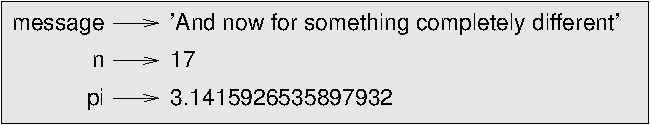
\includegraphics[scale=0.8]{figs/state2.pdf}}
\caption{State diagram.}
\label{fig.state2}
\end{figure}



\section{變量名}
\index{variable}

程式工程師一般會為變量起個容易理解記憶的名字, 使人一看即知其用途. 

變量名可長可短, 包含字母和數字, 但不能以數字開頭, 
大小寫均可用, 但是方便起見, 建議只用小寫字母. 

變量名也可以使用\verb"_",  多用在形如\verb"your_name" 或 
\verb"airspeed_of_unladen_swallow" 這種多單詞命名的變量名中. 
\index{underscore character}

如果變量名包含了非法字符, 就會語法錯誤:

\begin{verbatim}
>>> 76trombones = 'big parade'
SyntaxError: invalid syntax
>>> more@ = 1000000
SyntaxError: invalid syntax
>>> class = 'Advanced Theoretical Zymurgy'
SyntaxError: invalid syntax
\end{verbatim}
%
變量名 {\tt 76trombones}  的錯誤在於數字開頭, 
而{\tt more@} 是因為包含了不合法字符 {\tt @}. 
那麼 {\tt class} 為什麼也不正確呢?

這是因為 {\tt class} 是 Python的一個 {\bf 關鍵字}. 
解釋器用關鍵字(也稱預留字)來識別解析代碼, 所以關鍵字不能作為變量名使用. 
\index{keyword}

Python 3 包含以下關鍵字:

\begin{verbatim}
False      class      finally    is         return
None       continue   for        lambda     try
True       def        from       nonlocal   while
and        del        global     not        with
as         elif       if         or         yield
assert     else       import     pass
break      except     in         raise
\end{verbatim}
%

你無須刻意背誦這些關鍵字. 在多數開發環境中, 關鍵字會以特殊顏色標識, 
所以如果誤用作變量名時, 很容易發覺. 

\section{表達式和語句}

{\bf 表達式} 是值, 變量以及運算子的集合. 
值本身可以認為是表達式, 同樣, 變量本身也是. 
所以下面都可以認為是合法的表達式:
\index{expression}

\begin{verbatim}
>>> 42
42
>>> n
17
>>> n + 25
42
\end{verbatim}
%
當根據提示符輸入表達式時, 解釋器會進行 {\bf 估算}, 獲取表達式的值. 
上例中, {\tt n} 的值是17, {\tt n+25} 的值是42. 
\index{evaluate}

 {\bf 語句} 是代碼的基本有效單位, 例如新建變量或者輸出值. 
\index{statement}

\begin{verbatim}
>>> n = 17
>>> print(n)
\end{verbatim}
%
第一行是給 {\tt n} 賦值的賦值語句, 第二行是顯示 {\tt n}結果的輸出語句. 

鍵入語句, 解釋器根據語句規則{\bf 運行}, 通常, 語句沒有值({\bf 注意:表達式有值}). 
\index{execute}


\section{腳本模式}

截至當前, 我們一直使用 {\bf 交互模式}運行代碼, 
此模式需要不斷和解釋器交互. 
入門學習採用交互模式尚可行, 
但代碼行數一旦增多, 使用就會很麻煩. 
\index{interactive mode}

替代方案是將代碼保存至{\bf 腳本}文件, 然後解釋器在{\bf 腳本模式}
運行文件. 通俗來說, Python腳本以 {\tt .py} 結尾. 
\index{script}
\index{script mode}

了解了如何創建以及運行腳本, 便可開啟後續學習. 
如果沒有配套工具, 建議繼續採用PythonAnywhere. 
同時, 我已在\url{http://tinyurl.com/thinkpython2e}
撰寫了運行腳本模式的相關步驟. 

Python提供兩種模式, 在寫入腳本前, 
可以採用交互模式進行部分語句的驗證. 
但是兩種模式多有差異, 會令人無所適從. 
\index{interactive mode}
\index{script mode}

例如, 以Python進行運算, 可以鍵入:

\begin{verbatim}
>>> miles = 26.2
>>> miles * 1.61
42.182
\end{verbatim}

首行代碼給{\tt miles}賦值, 但是不顯示結果. 
第二行是表達式, 解釋器會解析執行, 並顯示結果, 約為42公里. 

但是在腳本模式同樣執行, 不會獲得輸出結果. 
表達式在腳本模式不會輸出結果, 如果需要顯示, 可以採用 {\tt print}語句:

\begin{verbatim}
miles = 26.2
print(miles * 1.61)
\end{verbatim}

初次使用, 會感到奇怪. 為了更深入了解, 
可以在Python解釋器鍵入以下內容, 看看現象:

\begin{verbatim}
5
x = 5
x + 1
\end{verbatim}

將同樣語句放入腳本並運行, 會如何?
如果將每個表達式都放入print語句中, 並運行, 又會如何?


\section{運算次序}
\index{order of operations}
\index{PEMDAS}

當表達式含有多個運算子時, 執行順序主要基於 {\bf 運算次序}. 
對於數學運算子, Python也遵循數學慣例. 
本書採用縮寫 {\bf PEMDAS} 來輔助記憶以下規則:

\begin{itemize}

\item 括號({\bf P}arentheses)優先, 可以據此調整運算次序. 
因為括號中的表達式會優先處理, 所以 {\tt 2 * (3-1)} 結果為 4, {\tt (1+1)**(5-2)} 則為 8. 
同時採用括號可以提高表達式的可讀性. 
比如,  {\tt (minute * 100) / 60}加上括號, 結果雖然沒有變化, 但是可讀性提高不少. 

\item 冪運算({\bf E}xponentiation)相對優先級更高. 所以
{\tt 1 + 2**3} 等於 9而非 27,  {\tt 2 * 3**2} 等於 18而非 36. 

\item 乘法({\bf M}ultiplication)和除法({\bf D}ivision)優先於加法({\bf A}ddition)
和減法({\bf S}ubtraction). 所以 {\tt 2*3-1} 等於 5而非4, {\tt 6+4/2} 等於 8而非 5. 

\item 對於同優先級的運算, 遵照自左向右的順序(除冪運算). 
 在{\tt degrees / 2 * pi}中, 先執行除法運算, 獲得的結果再乘以 {\tt pi}. 
如果想除以$2 \pi$,  可以使用括號處理或者改寫為{\tt degrees / 2 / pi}. 

\end{itemize}

不必強求記憶這些運算子的優先級, 碰到比較複雜的表達式, 採用括號會方便很多. 


\section{字符串操作}
\index{string!operation}
\index{operator!string}

通常, 字符串甚至類似數字的字符串的運算, 一般不能使用數學運算子, 
下面的表達式均是非法運算:

\begin{verbatim}
'chinese'-'food'    'eggs'/'easy'    'third'*'a charm'
\end{verbatim}
%

但是有兩個例外,  {\tt +} 和 {\tt *}. 

 {\tt +} 可以實現 {\bf 字符串拼接}, 也就是首尾相接. 例如:
\index{concatenation}

\begin{verbatim}
>>> first = 'throat'
>>> second = 'warbler'
>>> first + second
throatwarbler
\end{verbatim}
%
 {\tt *} 同樣可以作用於字符串, 表示堆疊. 例如\verb"'Spam'*3" 表示
\verb"'SpamSpamSpam'". 如果一個值是字符串, 另外一個值就需要是整數. 

{\tt +} 和 {\tt *}在字符串上的使用類似數值運算中的作用. 
 {\tt 4*3} 即是 {\tt 4+4+4}, 
而 \verb"'Spam'*3"  也等於 \verb"'Spam'+'Spam'+'Spam'". 
但是, 數字的加法和乘法與字符串的拼接和堆疊, 在某方面的應用會有明顯不同. 
你是否可以想到, 加法運算正常, 而字符串拼接卻表現截然不同的場景?

\index{commutativity}


\section{注釋}
\index{comment}

隨著代碼量越來越龐大, 越來越複雜, 閱讀並理解其邏輯也越來越困難. 
形式語言使用時又寫得密密麻麻, 對著滿頁代碼去明白其邏輯和功能, 便異常艱難. 

所以, 在程式代碼中加入一些自然語言來進行解釋, 說明其作用, 便顯得異常重要. 
這些解釋說明, 便叫做{\bf 注釋},  一般以井號( \verb"#") 開頭:

\begin{verbatim}
# 計算所占一小時的百分比
percentage = (minute * 100) / 60
\end{verbatim}
%
此例中, 注釋獨占一行. 你也可以把注釋寫在代碼末尾:

\begin{verbatim}
percentage = (minute * 100) / 60     # 所占一小時的百分比
\end{verbatim}
%
代碼中所有  {\tt \#} 開頭的行, 在執行過程中都會被忽略. 

編碼中實現特殊邏輯時, 注釋顯得尤為重要. 
要記住, 說明編碼的 {\em 緣由} , 遠勝於講述代碼的{\em 作用}. 

下面這條注釋便顯得多餘:

\begin{verbatim}
v = 5     # assign 5 to v
\end{verbatim}
%

而下面的注釋則包含了未體現在代碼中的有用信息:

\begin{verbatim}
v = 5     # 速度(米/秒) 
\end{verbatim}
%
好的變量命名可以減少注釋的使用, 但是變量名過長, 又顯得代碼繁雜而難以閱讀, 
所以如何取捨, 需要權衡. 


\section{調試}
\index{debugging}
\index{bug}

一般程式中會出現三種異常:
語法錯誤, 運行時錯誤以及語義錯誤. 
有效區分三者差異, 可以大大提高定位速度. 

\begin{description}

\item[語法錯誤:] "語法" 指代碼結構以及使用規範. 
例如, 括號必須成對出現, 
{\tt (1 + 2)}正確, 而{\tt 8)}便存在語法錯誤. 
\index{syntax error} 
\index{error!syntax}
\index{error message}
\index{syntax} 

如果程式存在語法錯誤, Python會直接報錯並退出執行, 
程式便無法繼續運行. 
開始學習編程時, 需要耗費大量精力跟蹤語法錯誤. 
隨著經驗增長, 此類錯誤會越來越少, 而定位也會越來越快. 


\item[運行時錯誤:] 運行時錯誤只有在程式開始運行後才會出現. 
這些錯誤也叫作{\bf 異常}, 因為一般表示異常或者壞的事情發生了. 
\index{runtime error} \index{error!runtime}
  \index{exception} \index{safe language} \index{language!safe}

本書前面幾章的程式較為簡單, 運行時錯誤也較少遇到, 
所以想窺其全貌, 還需一段時間. 

\item[語義錯誤:] 第三種錯誤是 "語義錯誤", 意如其字. 
如果代碼中存在語義錯誤, 代碼不會報錯, 只是無法得到預期的結果. 
具體來說, 便是會按照你的指示去做. 
\index{semantic error}
  \index{error!semantic} \index{error message}

語義錯誤的識別很棘手, 需要觀察輸出, 回溯代碼, 才能確定其邏輯. 

\end{description}


\section{術語表}

\begin{description}

\item[變量(variable):]  標識值的名稱. 
\index{variable}

\item[賦值(assignment):]  為變量賦值的語句. 
\index{assignment}

\item[狀態圖(state diagram):]  一堆變量和值的指向圖. 
\index{state diagram}

\item[關鍵字(keyword):]  編程語言用來解析代碼的預留字, 像 {\tt if}、{\tt  def} 和 {\tt while}, 
均不能作為變量名使用. 
\index{keyword}

\item[操作數(operand):]  運算子操作的單一值對象. 
\index{operand}

\item[表達式(expression):]  變量、運算子以及值的集合, 共同來表示單一結果. 
\index{expression}

\item[求值(evaluate):]  執行運算產生值, 從而簡化表達式的過程. 
\index{evaluate}

\item[語句(statement):]  表示命令或者操作的代碼塊. 目前遇到的語句包括賦值語句以及打印語句. 
\index{statement}

\item[執行(execute):]  通過執行計算來簡化表達式, 從而產生值.
\index{execute}

\item[交互模式(interactive mode):] 在Python解釋器中根據提示符進行代碼輸入的模式. 
\index{interactive mode}

\item[腳本模式(script mode):] 用Python解釋器讀取腳本並運行代碼的模式. 
\index{script mode}

\item[腳本(script):] 存儲代碼的文件. 
\index{script}

\item[運算次序(order of operations):]  包含多運算子和操作數的表達式執行時所遵循的先後順序. 
\index{order of operations}

\item[拼接(concatenate):]  操作數首位相接. 
\index{concatenation}

\item[注釋(comment):]  幫助他人理解代碼的有效信息, 對程式執行無影響. 
\index{comment}

\item[語法錯誤(syntax error):] 導致代碼無法解析(因此無法解釋)的錯誤. 
\index{syntax error}

\item[異常(exception):]  程式運行時遇到的錯誤. 
\index{exception}

\item[語義(semantics):]  代碼含義. 
\index{semantics}

\item[語義錯誤(semantic error):]   未獲得預期結果的錯誤. 
\index{semantic error}

\end{description}


\section{習題集}

\begin{exercise}

重申從上節便給出的建議, 學習新知識, 
盡量在交互模式下不斷試錯, 大膽假設, 小心求證. 

\begin{itemize}

\item 既然{\tt n = 42} 正確, 那麼{\tt 42 = n}呢?

\item {\tt x = y = 1}正確與否?

\item 在一些編程語言中, 每個語句都會以分號{\tt ;}結尾, 
如果在Python的語句末尾加上分號會怎樣?

\item 語句末尾加句號會如何?

\item 數學公式中, 可以用 $x y$ 表示 $x$ 和 $y$ 相乘. Python中若如此使用會如何?

\end{itemize}

\end{exercise}


\begin{exercise}

用Pyhton解釋器進行運算: 
\index{calculator}

\begin{enumerate}

\item 半徑$r$的球體體積是 $\frac{4}{3} \pi r^3$. 那半徑為5的球體體積是多少?

\item 假設書原價\$24.95, 但書店擁有 40\% 的折扣. 
同時郵寄首件需要郵費\$3, 後續每件75美分, 
如果批發60件, 總費用多少?

\item 如果我6:52離家, 以慢跑方式 (8分15秒/每英里)跑了1英里, 然後以
快跑方式(7分12秒/每英里)跑了3英里, 最後, 又以慢跑方式跑了1英里, 
那什麼時候到家?
\index{running pace}

\end{enumerate}
\end{exercise}


\chapter{函數}
\label{funcchap}

在編程領域, {\bf 函數} 是指執行既定運算的語句組合. 
定義函數便是確定名稱以及語句組合. 然後, 便可以通過函數名來"調用"函數. 
\index{function}

\section{函數調用}
\label{functionchap}
\index{function call}

上文已展示過{\bf 函數調用}

\begin{verbatim}
>>> type(42)
<class 'int'>
\end{verbatim}
%
此函數的名稱為{\tt type},  括號中的表達式叫做函數的{\bf 參數}. 
此處獲得的結果, 表示參數的類型. 
\index{parentheses!argument in}

通俗來說, 函數的作用便是根據 "輸入" 的參數, "返回" 相應的結果. 
這個結果也叫做{\bf 返回值}. 
\index{argument}
\index{return value}

Python提供了值類型轉換的函數, 正常情況下, {\tt int} 函數會將任意值轉為整型, 
除非輸入有誤:
\index{conversion!type}
\index{type conversion}
\index{int function}
\index{function!int}

\begin{verbatim}
>>> int('32')
32
>>> int('Hello')
ValueError: invalid literal for int(): Hello
\end{verbatim}
%
{\tt int} 雖然可以將浮點數轉為整數, 但是不會四捨五入, 而是直接捨去小數部分:

\begin{verbatim}
>>> int(3.99999)
3
>>> int(-2.3)
-2
\end{verbatim}
%
{\tt float} 會將整數以及字符串格式小數轉為浮點數:
\index{float function}
\index{function!float}

\begin{verbatim}
>>> float(32)
32.0
>>> float('3.14159')
3.14159
\end{verbatim}
%
最後, {\tt str} 會將任意輸入值轉為字符串:
\index{str function}
\index{function!str}

\begin{verbatim}
>>> str(32)
'32'
>>> str(3.14159)
'3.14159'
\end{verbatim}
%

\section{數學函數}
\index{math function}
\index{function!math}

Pyhton內置了數學模塊, 可以提供大部分的數學計算函數. 
{\bf 模塊}是指包含一類函數的文件. 
\index{module}
\index{module object}

在使用模塊中的函數前, 我們需要用 {\bf import 語句} 來導入模塊:

\begin{verbatim}
>>> import math
\end{verbatim}
%
導入語句會創建一個名為 {\tt math}的 {\bf 模塊對象}. 
輸入模塊對象名稱, 可以看到一些相關信息:

\begin{verbatim}
>>> math
<module 'math' (built-in)>
\end{verbatim}
%
模塊對象包含所有模塊中的函數和變量. 想調用相應函數, 需要調用模塊名和函數名, 
中間用點(也可以當作英文中的句號)來分隔. 這種調用方法, 就是{\bf 點標法}. 
\index{dot notation}

\begin{verbatim}
>>> ratio = signal_power / noise_power
>>> decibels = 10 * math.log10(ratio)

>>> radians = 0.7
>>> height = math.sin(radians)
\end{verbatim}
%
第一個例子使用 \verb"math.log10" 計算分貝信噪比(已知 \verb"signal_power" 和
\verb"noise_power"). 
math 模塊也提供了{\tt log}函數, 此函數是以{\tt e}為底. 
\index{log function}
\index{function!log}
\index{sine function}
\index{radian}
\index{trigonometric function}
\index{function!trigonometric}

第二個例子是計算{\tt 弧度(radians)}的正弦值. 
{\tt 弧度} 一般作為三角函數({\tt sin}, {\tt cos}和 {\tt tan}, 等)的輸入參數. 
而角度轉弧度, 需要除以180然後乘以$\pi$:

\begin{verbatim}
>>> degrees = 45
>>> radians = degrees / 180.0 * math.pi
>>> math.sin(radians)
0.707106781187
\end{verbatim}
%
{\tt math.pi} 表達式是從math模塊獲取變量 {\tt pi}, 這是一個 $\pi$的浮點格式近似值, 
精確到小數點後15位. 
\index{pi}

如果熟悉三角函數原理, 便可以通過與 $\frac{ \sqrt{2}} {2}$ 比較來驗證結果:
\index{sqrt function}
\index{function!sqrt}

\begin{verbatim}
>>> math.sqrt(2) / 2.0
0.707106781187
\end{verbatim}
%

\section{組合}
\index{composition}

目前, 我們學習了編程涉及的各個元素---變量, 表達式以及語句. 
但都是分開來講, 並未整合在一起. 

編程語言的強大之處在於, 可以構建眾多的小積木, 然後 {\bf 組合}起來. 
例如, 函數的參數既然可以寫各種表達式, 那便可以是算數運算:

\begin{verbatim}
x = math.sin(degrees / 360.0 * 2 * math.pi)
\end{verbatim}
%
也可以是函數調用:

\begin{verbatim}
x = math.exp(math.log(x+1))
\end{verbatim}
%
任何可以使用值的地方, 都可以使用表達式來替換, 除了一種情況:
賦值語句的左側必須是變量名. 
左側出現表達式會報語法錯誤(相關信息見後續章節). 

\begin{verbatim}
>>> minutes = hours * 60                 # right
>>> hours * 60 = minutes                 # wrong!
SyntaxError: can't assign to operator
\end{verbatim}
%
\index{SyntaxError}
\index{exception!SyntaxError}


\section{創建函數}

我們在Python編程中一直是使用函數, 現在可以嘗試創建一個函數. 
{\bf 函數定義} 一般指定義函數名以及調用時使用的語句組. 
\index{function}
\index{function definition}
\index{definition!function}

這是一個示例:

\begin{verbatim}
def print_lyrics():
    print("I'm a lumberjack, and I'm okay.")
    print("I sleep all night and I work all day.")
\end{verbatim}
%

{\tt def}關鍵字表示這是一個函數定義. 
函數名是 \verb"print_lyrics". 
函數名的命名規則和變量名命名規則一致:
可包含字母, 數字或下劃線, 首字母不能為數字. 
同時不能使用關鍵字作為函數名, 要避免變量和函數重名. 
\index{def keyword}
\index{keyword!def}
\index{argument}

函數名後的空括號表示沒有參數. 
\index{parentheses!empty}
\index{header}
\index{body}
\index{indentation}
\index{colon}

函數定義首行一般叫做 {\bf 函數頭}, 其他部分叫{\bf 函數體}.
函數頭以冒號結尾, 函數體必須縮進. 
依照慣例, 一個縮進等於四個空格. 
消息體可以包含任意行語句. 

print語句中的字符串需要被雙引號包著. 
一般單引號和雙引號作用相同, 所以人們多數情況使用單引號, 
除非字符串中本來就有單引號, 這種情況就要使用雙引號了. 

所有的引號(無論單雙)都是 ``直引號'', 就是鍵盤確認鍵(Enter)旁邊的那個, 
像本句中這種``彎引號'', 在Python使用中就是非法的. 

在交互模式下定義函數, 解釋器會輸出省略號({\tt ...}) 來提示函數定義尚未結束:
\index{ellipses}

\begin{verbatim}
>>> def print_lyrics():
...     print("I'm a lumberjack, and I'm okay.")
...     print("I sleep all night and I work all day.")
...
\end{verbatim}
%
想結束函數定義, 需要多敲一個換行. 

函數定義完成便會創建一個 \verb"function" 類型的 {\bf 函數對象}:
\index{function type}
\index{type!function}

\begin{verbatim}
>>> print(print_lyrics)
<function print_lyrics at 0xb7e99e9c>
>>> type(print_lyrics)
<class 'function'>
\end{verbatim}
%
調用自定義函數和調用內置函數的方式一樣:

\begin{verbatim}
>>> print_lyrics()
I'm a lumberjack, and I'm okay.
I sleep all night and I work all day.
\end{verbatim}
%
一旦函數定義完成, 便可在其他函數中使用. 比如, 為了避免重複, 
可以直接定義一個\verb"repeat_lyrics"函數:

\begin{verbatim}
def repeat_lyrics():
    print_lyrics()
    print_lyrics()
\end{verbatim}
%
然後調用 \verb"repeat_lyrics":

\begin{verbatim}
>>> repeat_lyrics()
I'm a lumberjack, and I'm okay.
I sleep all night and I work all day.
I'm a lumberjack, and I'm okay.
I sleep all night and I work all day.
\end{verbatim}
%
當然, 歌詞沒有這樣的. 

\section{定義和調用}
\index{function definition}

將上述代碼片段整理為一個完整程式:

\begin{verbatim}
def print_lyrics():
    print("I'm a lumberjack, and I'm okay.")
    print("I sleep all night and I work all day.")

def repeat_lyrics():
    print_lyrics()
    print_lyrics()

repeat_lyrics()
\end{verbatim}
%
此程式包含兩個函數:\verb"print_lyrics" 和 \verb"repeat_lyrics". 
這些函數定義的執行和其他語句一樣, 但是會在執行後創建函數對象. 
函數內的語句只有在函數調用時才會執行, 同時定義函數並不會輸出結果. 
\index{use before def}

如你所料, 函數運行前必須先定義函數, 也就是說, 
函數定義語句先執行, 函數才能被調用. 

練習一下, 將程式的末行提到開始, 令函數先被調用, 再被定義. 
運行程式, 看看會報什麼錯誤. 

將函數調用再次移回末尾, 然後將 \verb"print_lyrics" 函數定義
放到 \verb"repeat_lyrics" 函數的後面, 看看程式運行時, 會發生什麼?

\section{運行流程}
\index{flow of execution}

為保證函數定義先於函數調用, 需要了解語句執行順序, 
也叫做{\bf 運行流程 }. 

程式代碼從第一行開始, 從上到下, 逐行運行. 

執行函數的定義不會改變代碼邏輯運行順序, 
但是要謹記, 函數內的語句只會在函數被調用時才執行. 

函數調用就像在代碼運行流程中繞路一樣, 不會繼續向下執行語句, 
而是跳轉到函數體內, 運行內部語句, 完成後再回到離開的地方. 

聽起來很簡單, 但是要意識到, 函數可以不斷調用函數({\tt 譯者註:類似套娃}).
甲函數運行中, 可能會調用乙函數, 從而去執行其語句, 
然後乙函數運行中又可能去調用其他函數!

幸虧Python 解釋器能夠有效追蹤函數的執行流程, 才可以在函數執行完成後, 
回到函數調用的地方, 從而繼續執行, 直到結束. 

所以, 不要簡單地從上到下閱讀程式, 
有時候更要關注代碼運行流程. 


\section{形參和實參}
\label{parameters}
\index{parameter}
\index{function parameter}
\index{argument}
\index{function argument}

我們觀察到有些函數需要參數. 例如調用{\tt math.sin}函數, 需要傳遞數值作為參數. 
還有些函數不止一個參數:{\tt math.pow} 需要兩個參數, 分別是底和冪. 

函數內, 實參會被賦值給{\bf 形參}. 
下面是函數傳參(實參賦值給形參)的定義:
\index{parentheses!parameters in}

\begin{verbatim}
def print_twice(bruce):
    print(bruce)
    print(bruce)
\end{verbatim}
%
此函數會將實參賦值給形參 {\tt bruce}, 當此函數被調用時, 
會輸出兩次參數值(無論參數為何). 

此函數適用於任何可被打印的值. 

\begin{verbatim}
>>> print_twice('Spam')
Spam
Spam
>>> print_twice(42)
42
42
>>> print_twice(math.pi)
3.14159265359
3.14159265359
\end{verbatim}
%
自定義函數和內置函數的適用規則是一致的, 
所以\verb"print_twice"的實參也可以是任意表達式:
\index{composition}
\index{programmer-defined function}
\index{function!programmer defined}

\begin{verbatim}
>>> print_twice('Spam '*4)
Spam Spam Spam Spam
Spam Spam Spam Spam
>>> print_twice(math.cos(math.pi))
-1.0
-1.0
\end{verbatim}
%
實參在函數調用前運行, 所以在上例中, 表達式 \verb"'Spam '*4" 和
{\tt math.cos(math.pi)} 只會運行一次. 
\index{argument}

也可以使用變量作為實參:

\begin{verbatim}
>>> michael = 'Eric, the half a bee.'
>>> print_twice(michael)
Eric, the half a bee.
Eric, the half a bee.
\end{verbatim}
%
函數實參的變量命名 ({\tt michael})和函數形參的命名({\tt bruce})毫無關聯. 
無論外部傳遞進來的值如何命名, 函數 \verb"print_twice"內部, 我們統稱其為 {\tt bruce}. 


\section{局部變量和參數}
\index{local variable}
\index{variable!local}

函數內部定義的變量都是{\bf 局部}的, 也就是說, 只能作用於函數內部, 例如:
\index{parentheses!parameters in}

\begin{verbatim}
def cat_twice(part1, part2):
    cat = part1 + part2
    print_twice(cat)
\end{verbatim}
%
此函數將兩個參數拼接後, 結果輸出兩次. 以下是用例:
\index{concatenation}

\begin{verbatim}
>>> line1 = 'Bing tiddle '
>>> line2 = 'tiddle bang.'
>>> cat_twice(line1, line2)
Bing tiddle tiddle bang.
Bing tiddle tiddle bang.
\end{verbatim}
%
\verb"cat_twice"運行結束, 內部變量{\tt cat}便被銷毀. 
如果現在嘗試輸出它, 會報錯:
\index{NameError}
\index{exception!NameError}

\begin{verbatim}
>>> print(cat)
NameError: name 'cat' is not defined
\end{verbatim}
%
形參都是局部使用的, 例如 {\tt bruce} 變量便不會出現在 \verb"print_twice" 函數之外.
\index{parameter}


\section{堆疊圖}
\label{stackdiagram}
\index{stack diagram}
\index{function frame}
\index{frame}
若想跟蹤變量使用情況, 一般繪製{\bf 堆疊圖}比較有效. 
和狀態圖類似, 堆疊圖也會標識每個變量的值, 不同之處是, 
堆疊圖會標識變量所屬函數. 
\index{stack diagram}
\index{diagram!stack}

每個函數都用一個{\bf 框} 來表示, 一個框就是一個旁邊有函數名, 
內部是參數以及變量值的箱體圖. 
前述例子的箱體圖見圖~\ref{fig.stack}. 

\begin{figure}
\centerline
{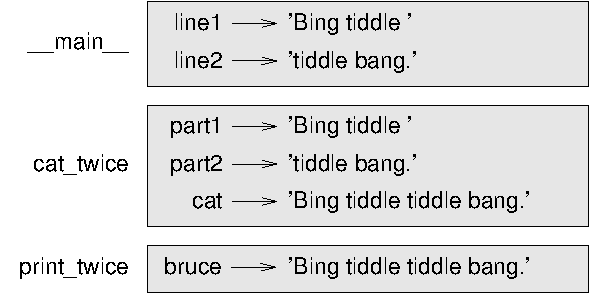
\includegraphics[scale=0.8]{figs/stack.pdf}}
\caption{堆疊圖.}
\label{fig.stack}
\end{figure}

堆疊圖中的各個框的排列方式標示了各個函數的調用關係. 
此例中, \verb"print_twice"函數被 \verb"cat_twice"調用, 
\verb"cat_twice" 被\verb"__main__"調用. \verb"__main__"是
頂層框的一個特殊名字, 任何函數外的變量, 都屬於它. 
\index{main}

形參和實參一一對應, 所以{\tt part1} 和{\tt line1}的值相同, 
{\tt part2} 和{\tt line2}的值也相同, 並且, 
 {\tt bruce} 和{\tt cat}的值也一樣. 

如果函數在調用過程中出錯, Python會輸出此函數名稱, 
以及調用它的上級函數信息, 以及更上級的函數, 一直到 \verb"__main__" 函數.

例如, 如果在\verb"print_twice" 中調用{\tt cat}, 會得到名稱異常({\tt NameError}):

\begin{verbatim}
Traceback (innermost last):
  File "test.py", line 13, in __main__
    cat_twice(line1, line2)
  File "test.py", line 5, in cat_twice
    print_twice(cat)
  File "test.py", line 9, in print_twice
    print(cat)
NameError: name 'cat' is not defined
\end{verbatim}
%
這一系列跟蹤函數的信息叫做{\bf 溯源}, 這些信息會顯示是哪個文件出錯, 哪行出錯, 
以及運行時函數, 甚至引起錯誤的代碼行號. 
\index{traceback}

在溯源信息中的函數次序和堆疊圖中的框的次序是一致的, 
當前正在運行的函數都是在最下面. 

\section{有值函數和無值函數}
\index{fruitful function}
\index{void function}
\index{function!fruitful}
\index{function!void} 

目前用到過的一些函數, 例如數學函數, 都會返回結果, 
一得之見, 暫稱{\bf 有值函數}. 其他函數, 像 \verb"print_twice", 
運行完成, 並不會返回值, 便叫做{\bf 無值函數}. 

當調用有值函數時, 一般是希望對返回結果另行處理, 比如, 
賦值結果到某個變量, 或者置於表達式中使用:

\begin{verbatim}
x = math.cos(radians)
golden = (math.sqrt(5) + 1) / 2
\end{verbatim}
%
在交互模式調用函數, Python解釋器會輸出結果:

\begin{verbatim}
>>> math.sqrt(5)
2.2360679774997898
\end{verbatim}
%
但是在腳本模式, 調用有值函數, 卻永遠不會看到返回值!

\begin{verbatim}
math.sqrt(5)
\end{verbatim}
%
這個腳本文件主要計算5的平方根, 但因為沒有保存或者顯示結果, 所以不是很有用. 
\index{interactive mode}
\index{script mode}

無值函數可以在屏幕顯示信息或者製造其他效果, 
只是不會有返回值. 如果將函數運行結果賦值到某個變量, 
那變量會指向一個特殊的值:{\tt None}.
\index{None special value}
\index{special value!None}

\begin{verbatim}
>>> result = print_twice('Bing')
Bing
Bing
>>> print(result)
None
\end{verbatim}
%
{\tt None}是個具有既定類型的特殊值, 和字符串 \verb"'None'"是不同的:

\begin{verbatim}
>>> type(None)
<class 'NoneType'>
\end{verbatim}
%
目前我們定義的函數都是無返回值的, 後續章節將開始定義有返回值的函數. 
\index{NoneType type}
\index{type!NoneType}


\section{函數何用}
\index{function!reasons for}

將程式劃分為一個個函數是否值得, 對此的考量, 可以參看以下緣由:

\begin{itemize}

\item 函數可以將一組語句歸為一類, 便於閱讀和調試. 

\item 函數可以消除重複, 簡化代碼, 針對功能, 修改一處即可. 

\item 將程式切分為函數, 可以分別調試, 然後組合它們即可. 

\item 設計良好的函數可以編寫一次, 調試一次, 多處調用, 有效復用. 

\end{itemize}


\section{調試}

編程最重要的技能之一就是調試了, 雖往往令人黯然神傷, 愁眉難舒, 
卻是編程中最考驗才智, 最富有挑戰以及最有趣的地方.
\index{experimental debugging}
\index{debugging!experimental}

在某些方面, 調試和偵探工作很像. 面對線索, 有效推理, 確定造就結果的流程和緣由. 

調試又像實驗科學, 針對問題, 一旦有所想法, 便可修改程式, 再次嘗試. 
如果假設正確, 便可預期修改後的結果, 向可執行的程式代碼推進. 
如果假設錯誤, 便要繼續探究了. 正如Sherlock Holmes(夏洛克·福爾摩斯)所說, 
``除去所有不可能因素, 留下來的東西, 無論多麼不願意相信, 但這就是事實
的真相."(A. Conan Doyle, {\em The Sign of Four})
\index{Holmes, Sherlock}
\index{Doyle, Arthur Conan}

對某些人而言, 編程便是調試. 這是因為, 編程便是不斷調試程式, 直到實現目標的過程. 
所以, 建議先寫可執行代碼, 然後逐步修改並調試程式, 進而實現預定效果. 

比如, Linux 操作系統具有數百萬行代碼,  但它起源於Linus Torvalds
研究Intel 80386芯片的一段簡單代碼. 據Larry Greenfield所說, 
``Linus的早期項目中, 有個程式是在AAAA和BBBB之間交替輸出, 而這後來演化為了Linux.''
({\em The Linux Users' Guide} Beta Version 1).
\index{Linux}


\section{術語表}

\begin{description}

\item[函數(function):] 特別命名的一堆語句的組合, 實現特定功能. 可以有參數, 
也可以沒有參數, 可以返回值, 也可以不返回. 
\index{function}

\item[函數定義(function definition):]  創建函數的語句, 確定名稱, 參數以及內部語句. 
\index{function definition}

\item[函數對象(function object):]  函數定義運行後的值, 函數名便是指向函數對象的變量. 
\index{function object}

\item[函數頭(header):] 函數定義的首行.
\index{header}

\item[函數體(body):] 函數定義的內部語句.
\index{body}

\item[形參(parameter):] 函數內部用於表示傳入參數的名稱. 
\index{parameter}

\item[函數調用(function call):] 運行函數的語句, 由函數名, 以及括號中的參數串列構成. 
\index{function call}

\item[實參(argument):]  函數調用時傳入函數的值. 這個值會賦值給函數內部的形參. 
\index{argument}

\item[局部變量(local variable):]  函數內部變量, 局部變量只能在函數內部使用. 
\index{local variable}

\item[返回值(return value):]  函數返回的結果. 如果用函數調用作為表達式, 那麼函數返回值, 便是表達式的結果. 
\index{return value}

\item[有值返回(fruitful function):] 有返回值的函數. 
\index{fruitful function}

\item[無值返回(void function:] 返回值為 {\tt None}的函數. 
\index{void function}

\item[空值({\tt None}):] 無值返回函數返回的結果. 
\index{None special value}
\index{special value!None}

\item[模塊(module):] 包含相關函數以及定義的文件. 
\index{module}

\item[導入語句(import statement):] 讀取模塊文件並創建模塊對象的語句. 
\index{import statement}
\index{statement!import}

\item[模塊對象(module object):]  {\tt import}語句創建的值, 通過其可以獲取模塊內部的值. 
\index{module object}

\item[點標法(dot notation):]  通過在模塊名後緊跟一個點(英文句號)和要調用的函數名, 
來調用模塊函數的語法. 
\index{dot notation}

\item[組合(composition):] 採用簡單表達式構建複雜表達式, 簡單語句塑造複雜模塊的方法. 
\index{composition}

\item[運行流程(flow of execution):] 語句運行的順序.
\index{flow of execution}

\item[堆疊圖(stack diagram):]  表示函數,變量,以及值的關係圖. 
\index{stack diagram}

\item[框(frame):]  堆疊圖中表示函數調用的箱體圖,包括局部變量以及參數. 
\index{function frame}
\index{frame}

\item[溯源(traceback):] 異常發生時, 輸出相關運行函數信息的過程. 
\index{traceback}


\end{description}


\section{習題集}

\begin{exercise}
\index{len function}
\index{function!len}

書寫名為 \verb"right_justify" 同時以字符串{\tt s}為參數的函數, 
其輸出的字符串左側有足夠的空格, 以使輸出結果的最後一個字符在第70字符處. 

\begin{verbatim}
>>> right_justify('monty')
                                                                 monty
\end{verbatim}

提示: 使用字符串拼接以及堆疊. 此外, Python提供了內置函數{\tt len}, 可以返回字符串長度, 
例如, \verb"len('monty')"的結果為5.

\end{exercise}


\begin{exercise}
\index{function object}
\index{object!function}

函數對象可以賦值給變量, 或者作為實參傳遞. 
例如, \verb"do_twice" 便將函數對象作為參數傳入, 並調用了兩次:

\begin{verbatim}
def do_twice(f):
    f()
    f()
\end{verbatim}

下面是使用 \verb"do_twice"來調用兩次 \verb"print_spam" 的例子. 

\begin{verbatim}
def print_spam():
    print('spam')

do_twice(print_spam)
\end{verbatim}

\begin{enumerate}

\item 將上述代碼寫入腳本進行測試.

\item 修改 \verb"do_twice", 給其傳入兩個參數:函數對象和值, 
使其調用兩次傳入的函數對象, 這個函數對象會以傳入的值為參數.

\item 將本章\verb"print_twice"代碼複製到腳本.

\item 用新版 \verb"do_twice"函數調用 \verb"print_twice"兩次, 
並傳入參數 \verb"'spam'".

\item 定義新函數\verb"do_four", 令其接收函數對象和值, 
並以值為參數調用四次函數對象. 
要求函數體只有兩條語句, 而不是四條. 

\end{enumerate}

答案: \url{http://thinkpython2.com/code/do_four.py}.

\end{exercise}



\begin{exercise}

說明: 此習題只涉及已學過的語句和功能. 

\begin{enumerate}

\item 編寫繪製下面網格圖的函數:
\index{grid}

\begin{verbatim}
+ - - - - + - - - - +
|         |         |
|         |         |
|         |         |
|         |         |
+ - - - - + - - - - +
|         |         |
|         |         |
|         |         |
|         |         |
+ - - - - + - - - - +
\end{verbatim}
%
提示: 想要一行輸出多個值, 可以向print傳入多個值, 將值用逗號分隔:

\begin{verbatim}
print('+', '-')
\end{verbatim}
%
一般{\tt print}函數會附帶換行符, 但可以對其進行調整, 
使其以空格結尾, 如下:

\begin{verbatim}
print('+', end=' ')
print('-')
\end{verbatim}
%
上邊語句會將\verb"'+ -'"在同一行輸出, 如果再有print語句, 則會另起一行. 

\item 編寫繪製四行四列類似網格的函數. 

\end{enumerate}

答案: \url{http://thinkpython2.com/code/grid.py}.
致謝: 此習題基於 Oualline書中的習題
({\em Practical C Programming, Third Edition},  
O'Reilly Media, 1997).

\end{exercise}


\chapter{案例分析: 介面設計}
\label{turtlechap}

本章採用案例來講述, 如何設計可以協同運行的函數. 

主要介紹 {\tt turtle(烏龜)}模塊, 可以讓你用其繪圖功能, 製作圖片. 
大部分Python安裝包會預裝{\tt turtle} 模塊, 但如果你使用的是PythonAnywhere網站, 
現在還無法執行turtle示例(至少創作本書時還不能). 

如果你的計算機安裝了Python,  便可以直接運行這些實例. 
如果還沒有, 那麼最好現在安裝吧, 可以參看我寫的
操作步驟\url{http://tinyurl.com/thinkpython2e}. 

本章的代碼樣例可以從\url{http://thinkpython2.com/code/polygon.py}獲取. 


\section{模塊turtle}
\label{turtle}

打開Python解釋器, 鍵入以下命令, 以檢查是否安裝 {\tt turtle}模塊:

\begin{verbatim}
>>> import turtle
>>> bob = turtle.Turtle()
\end{verbatim}

運行此代碼, 會創建一個窗口, 此窗口包含一個箭頭, 代表一隻小烏龜. 
關閉窗口. 

創建名為{\tt mypolygon.py} 的文件, 並輸入以下代碼:

\begin{verbatim}
import turtle
bob = turtle.Turtle()
print(bob)
turtle.mainloop()
\end{verbatim}
%
 {\tt turtle}模塊(小寫字母 't')提供了函數{\tt Turtle} (大寫字母 'T'), 
它創建了Turtle 對象, 並將其賦值給名為 {\tt bob} 的變量. 
輸出{\tt bob}信息如下:

\begin{verbatim}
<turtle.Turtle object at 0xb7bfbf4c>
\end{verbatim}
%
這意味著{\tt bob}指向了{\tt turtle}模塊中{\tt Turtle}類型的對象.

\verb"mainloop" 會令窗口等待, 以執行其他操作. 但是本例
只需關閉窗口, 暫不進行其他操作. 

一旦創建了Turtle對象, 便可以調用{\bf 方法}在窗口中移動它. 
方法和函數類似, 但是略有不同. 比如, 令小烏龜前進:

\begin{verbatim}
bob.fd(100)
\end{verbatim}
%
方法{\tt fd}來自於烏龜對象{\tt bob}. 
調用方法就好比遞交申請:請求{\tt bob}向前移動. 

{\tt fd} 的參數是像素距離, 實際距離要看屏幕尺寸. 

其他可以調用的方法還有{\tt bk}, 實現向後移動, 
{\tt lt}實現左轉, {\tt rt}實現右轉. 
{\tt lt} 和 {\tt rt}的參數都是以度為單位的角度. 

同時, 每個烏龜都帶著筆, 可以抬起或落下;
如果筆落下, 烏龜移動時會留下痕跡. 
{\tt pu}和{\tt pd}方法分別代表``抬筆(pen up)''和``落筆(pen down)''.

將下面代碼加入程式, 以實現繪製直角(
創建{\tt bob}對象後, 調用\verb"mainloop"前):

\begin{verbatim}
bob.fd(100)
bob.lt(90)
bob.fd(100)
\end{verbatim}
%
運行程式, 可以看到{\tt bob}對象會向東移動, 然後向北移動, 並留下兩根垂直線段. 

現在嘗試繪製個正方形, 先不要著急學習下面的內容. 

%\newpage

\section{簡單重複}
\label{repetition}
\index{repetition}

我猜你會寫成下面的樣子:

\begin{verbatim}
bob.fd(100)
bob.lt(90)

bob.fd(100)
bob.lt(90)

bob.fd(100)
bob.lt(90)

bob.fd(100)
\end{verbatim}
%
用 {\tt for} 語句可以更加簡單地實現同樣的效果. 
將下面代碼寫入 {\tt mypolygon.py} 並運行::
\index{for loop}
\index{loop!for}
\index{statement!for}

\begin{verbatim}
for i in range(4):
    print('Hello!')
\end{verbatim}
%
所見如下:

\begin{verbatim}
Hello!
Hello!
Hello!
Hello!
\end{verbatim}
%
這是{\tt for}語句的簡單使用, 後面會講更多用法. 
但這些已足夠令我們重寫繪製方塊的程式了. 
暫時不要看下面的內容, 先嘗試一下. 

以下用{\tt for}語句實現繪製正方形:

\begin{verbatim}
for i in range(4):
    bob.fd(100)
    bob.lt(90)
\end{verbatim}
%
語句{\tt for} 的語法使用類似函數定義. 
以冒號結尾的語句為函數頭, 
縮進的內容為函數體. 
函數體可以是任意行語句. 

 {\tt for} 語句也叫 {\bf 迴圈}, 因為代碼執行流程會重複執行迴圈體, 
此例中, 會執行四次迴圈體.
\index{loop}

這一版代碼和上一版略有不同, 繪製完最後一條線後, 會多一次轉向. 
雖然多的這一步操作增加了耗時, 但是利用迴圈, 使重複操作更加簡單. 
當然, 這也令小烏龜回到了開始的地方, 朝向了開始的方向. 

\section{習題集}
以下為一系列操作{\tt turtle} 模塊的練習. 
雖然是為了讓大家高興一下, 但是也有別出心裁的地方, 
做練習的時候, 要好好思考一下醉翁之意. 

習題後面有答案, 但是盡量在完成或者盡力嘗試後再看. 

\begin{enumerate}

\item 編寫{\tt square}函數, 參數是個turtle對象{\tt t}, 用turtle繪製正方形. 

編寫函數, 將{\tt bob} 作為參數傳給{\tt square}, 然後運行程式. 

\item 為 {\tt square}添加參數{\tt length}, 令邊的長度為{\tt length}, 
同時修改函數, 令其調用第二個實參. 再次運行程式, 給{\tt length} 賦不同的值進行測試. 

\item 複製{\tt square}並命名為 {\tt polygon} . 添加參數{\tt n},
令其繪製正n邊形. 提示:正n邊形外角角度為$360/n$度. 
\index{polygon function} 
\index{function!polygon}

\item 編寫{\tt circle} 函數, 以turtle類型的{\tt t}, 以及半徑{\tt r}為參數, 
通過調用{\tt polygon}函數, 輸入適當長度和邊數, 繪製一個近似的圓形. 
用不同的 {\tt r}值, 測試程式. \index{circle function} \index{function!circle}

提示: 確定圓的周長, 使其滿足{\tt 邊長 * 邊數 = 周長}.

\item 升級{\tt circle}版本, 命名為{\tt arc}, 新增參數 {\tt angle}, 
用此值確定所繪製的圓弧的大小. 
 {\tt angle}以度為單位, 當 {\tt angle=360}, {\tt arc}會繪製一個完整的圓. 
\index{arc function}
\index{function!arc}

\end{enumerate}


\section{封裝}

第一道題是編寫繪製正方形的函數代碼, 調用函數, 傳遞turtle參數. 
代碼如下:

\begin{verbatim}
def square(t):
    for i in range(4):
        t.fd(100)
        t.lt(90)

square(bob)
\end{verbatim}
%
函數內的 {\tt fd} 和 {\tt lt}縮進兩次, 表示運行於函數定義裡面的{\tt for} 迴圈中. 
下一行 {\tt square(bob)}, 左邊距對齊同時沒有縮進, 
表示上面的 {\tt for} 迴圈以及函數定義都已結束. 

函數內的 {\tt t} 和 {\tt bob}指向的是同一個烏龜對象, 
因此{\tt t.lt(90)}就好比 {\tt bob.lt(90)}. 
那麼為何不直接用變量 {\tt bob}呢?
這是因為{\tt t}可以代指任意烏龜對象, 而不僅僅是 {\tt bob}, 
因此也可以再創建一個烏龜對象, 並作為參數傳入 {\tt square}:

\begin{verbatim}
alice = turtle.Turtle()
square(alice)
\end{verbatim}
%
將一段代碼寫在函數中, 叫做{\bf 封裝}. 
封裝的好處之一在於, 用一個簡單的名字來指代一段代碼, 類似文檔說明. 
另一個好處是可以復用代碼, 複製黏貼大段的代碼, 總是
不如復用代碼更顯簡潔!
\index{encapsulation}


\section{泛化}

下一步是給{\tt square}增加參數 {\tt length} , 詳見樣例:

\begin{verbatim}
def square(t, length):
    for i in range(4):
        t.fd(length)
        t.lt(90)

square(bob, 100)
\end{verbatim}
%
給函數增加參數, 叫做{\bf 泛化}. 
因為可以令函數使用場景更加廣泛:
上版代碼中, 正方形的邊長總是同一個值, 
而此版, 邊長可以是任意值.
\index{generalization}

下一步也是泛化. 
不再是只繪製正方形, {\tt polygon} 可以繪製任意多邊形, 詳見示例:

\begin{verbatim}
def polygon(t, n, length):
    angle = 360 / n
    for i in range(n):
        t.fd(length)
        t.lt(angle)

polygon(bob, 7, 70)
\end{verbatim}
%
上面代碼繪製了邊長為70的正七邊形. 

如果你使用的是Python 2, {\tt angle} 的值可能因為整除而出現偏差. 
有個簡單的辦法, 便是{\tt angle = 360.0 / n}. 分子為浮點數, 結果便也是浮點數了. 
\index{Python 2}

當函數有多個數值參數時, 很容易混淆各自代表什麼, 以及參數順序. 
所以比較好的辦法, 便是在傳遞實參串列時, 附上形參的名字:

\begin{verbatim}
polygon(bob, n=7, length=70)
\end{verbatim}
%
這也叫做{\bf 關鍵字參數}, 因為是把形參的名字作為 ``關鍵字''包含進來. 
(不要同Python中 {\tt while}和{\tt def}這種內置關鍵字混淆). 
\index{keyword argument}
\index{argument!keyword}

這種語法令程式可讀性更強. 同時也提示了實參和形參如何生效:
調用函數時, 實參賦值給了形參. 


\section{介面設計}

下一步要編寫 {\tt circle}, 此函數以半徑{\tt r}為參數. 
以下是採用{\tt polygon}來繪製正五十邊形的代碼:

\begin{verbatim}
import math

def circle(t, r):
    circumference = 2 * math.pi * r
    n = 50
    length = circumference / n
    polygon(t, n, length)
\end{verbatim}
%
首行根據公式 $2 \pi r$和半徑{\tt r} 計算圓的周長. 
要使用{\tt math.pi},  需要先導入{\tt math}. 
通常把 {\tt import}語句作為腳本的開始. 

{\tt n}是要逼近圓的正多邊形的邊數, {\tt length} 表示邊長. 
最後,  {\tt polygon}通過繪製正五十邊形, 來逼近半徑 {\tt r}的圓. 

此代碼的局限性在於, {\tt n} 是一個常量, 這表示繪製大的圓時, 線段過長. 
而繪製小圓時, 需要耗費時間繪製小線段. 
要想使此函數通用, 可以將{\tt n}作為函數的參數. 
這樣用戶( {\tt circle}的調用者)便可以更方便地使用, 但是介面會顯得不那麼簡潔了. 
\index{interface}

函數{\bf 介面} 是函數用途的簡介: 參數是什麼?函數做什麼?返回什麼?
如果一個介面聚焦於特定功能, 而非無關細節, 那麼這個介面就是``簡潔''的. 

這個案例中, {\tt r}放在介面中合適, 是因為要用它來確定圓的大小. 
而{\tt n}放進介面則顯得不太友好, 是因為它只與{\em 如何}繪製圓的細節有關. 

與其令介面複雜, 不如根據{\tt 周長}來確定一個合適的{\tt n}:

\begin{verbatim}
def circle(t, r):
    circumference = 2 * math.pi * r
    n = int(circumference / 3) + 3
    length = circumference / n
    polygon(t, n, length)
\end{verbatim}
%
現在邊的個數便是近似 {\tt circumference/3}的整數, 
每個邊的長度也就近似於3了, 用這個長度, 繪製大圓快速, 小圓好看, 
對任意尺寸的圓都適用. 

給{\tt n}加3是為了保證多邊形至少有3條邊. 

\section{重構}
\label{refactoring}
\index{refactoring}

我們可以復用{\tt polygon}來構造{\tt circle}, 是因為邊足夠多的正多邊形近似於圓. 
但是, 構造 {\tt arc}就不適合了, 因為沒有辦法用 {\tt polygon}或者{\tt circle}來繪製一段弧線. 

一個替代策略是複製{\tt polygon} ,  修改為{\tt arc}, 代碼如下:

\begin{verbatim}
def arc(t, r, angle):
    arc_length = 2 * math.pi * r * angle / 360
    n = int(arc_length / 3) + 1
    step_length = arc_length / n
    step_angle = angle / n
    
    for i in range(n):
        t.fd(step_length)
        t.lt(step_angle)
\end{verbatim}
%
函數後半段和 {\tt polygon}很像, 但如果我們不調整介面, 便無法復用 {\tt polygon}. 
我們需要給 {\tt polygon} 加入角度作為第三個參數, 來使其通用, 
那麼也不能繼續使用 {\tt polygon}作為名字了!反而叫{\tt polyline}會更合適些:

\begin{verbatim}
def polyline(t, n, length, angle):
    for i in range(n):
        t.fd(length)
        t.lt(angle)
\end{verbatim}
%
現在我們可以用 {\tt polyline}來重寫{\tt polygon} 和 {\tt arc}了:

\begin{verbatim}
def polygon(t, n, length):
    angle = 360.0 / n
    polyline(t, n, length, angle)

def arc(t, r, angle):
    arc_length = 2 * math.pi * r * angle / 360
    n = int(arc_length / 3) + 1
    step_length = arc_length / n
    step_angle = float(angle) / n
    polyline(t, n, step_length, step_angle)
\end{verbatim}
%
最後, 我們再用{\tt arc}來優化 {\tt circle} :

\begin{verbatim}
def circle(t, r):
    arc(t, r, 360)
\end{verbatim}
%
此過程---調整代碼, 優化介面, 便於復用---叫做{\bf 重構}. 
此案例中, 我們發現{\tt arc}和{\tt polygon}具有一些相似代碼, 
所以將其``抽離''為{\tt polyline}.\
\index{refactoring}

如果早有規劃, 我們可能會優先編寫{\tt polyline}, 避免後續耗時重構. 
但一般你很難在項目開始的時候, 便深入了解一切, 規劃好所有介面. 
只有開始編碼, 你才會更好地研究並理解其中曲折. 
所以, 有時候重構的過程也是你學習新知識的歷程. 


\section{開發計劃}
\index{development plan!encapsulation and generalization}

{\bf 開發計劃}便是指編碼的流程. 以上案例中, 我們採用的流程便是
``封裝和泛化'', 詳細步驟如下:

\begin{enumerate}

\item 先不考慮函數定義, 寫段小程式.

\item 如果代碼可用, 抽離相關代碼, 封裝進函數, 並命名.

\item 增加合適參數, 泛化函數.

\item 重複步驟1-3, 盡量抽離各個函數, 盡量複製黏貼, 減少打字(以及重複調試).

\item 嘗試重構程式. 比如, 在多個地方有相似代碼, 試試能否將其
拆解為恰當的通用函數.

\end{enumerate}

這種流程存在一定的缺點---後續會講述一些替代方案---但是在你無法提前規劃, 
如何將程式拆解為函數時, 這種方法可以讓你再編碼的同時優化程式. 

\section{幫助文檔}
\label{docstring}
\index{docstring}
{\bf 幫助文檔}是指函數開頭部分, 用來對介面(``doc''是``documentation''的簡稱)
進行解釋說明的文檔. 下面是個例子:

\begin{verbatim}
def polyline(t, n, length, angle):
    """Draws n line segments with the given length and
    angle (in degrees) between them.  t is a turtle.
    """    
    for i in range(n):
        t.fd(length)
        t.lt(angle)
\end{verbatim}
%
一般幫助文檔都要用三引號引起來, 也叫多行字符串, 
因為三引號允許字符串跨行. 
\index{quotation mark}
\index{triple-quoted string}
\index{string!triple-quoted}
\index{multiline string}
\index{string!multiline}

幫助文檔雖然簡潔, 但是重要, 因為它包含函數使用的相關說明. 
同時簡要概括了函數的功能(無需探查函數細節實現), 
以及各個參數的類型和作用, 以及應用場景. 

設計介面, 重要的一步, 便是編寫友好的幫助文檔. 
一個設計優良的介面, 應該是易於理解的;
如果需要耗費大量口舌講解, 那麼這個介面還有待優化. 


\section{調試}
\index{debugging}
\index{interface}

介面類似於調用方和函數之間的中間人. 
調用方提供特定參數, 函數執行特定操作. 

例如,  {\tt polyline}需要四個參數 : Turtle對象{\tt t},  整數{\tt n}, 
正數{\tt length},  以及以度為單位的數字{\tt angle}.

這些條件, 叫做 {\bf 前置條件},  因為這些條件滿足了, 函數才能執行. 
相反, 函數結尾的內容叫做{\bf 後置條件}. 後置條件包括函數預期效果
(比如繪製線段),  以及意外情況(移動Turtle或其他影響).
\index{precondition}
\index{postcondition}

前置條件是調用方的任務. 如果調用方違背(標註詳細的)前置條件, 導致函數異常, 
那麼責任在於調用方, 而不是函數. 

如果前置條件都滿足而後置條件未達到預期, 那問題便出在函數中. 
如果前置和後置條件都清晰明了, 那麼調試會方便很多. 

\section{術語表}

\begin{description}

\item[方法(method):] 用句點於對象連接的函數. 
\index{method}

\item[迴圈(loop):] 程式中可以重複執行的部分. 
\index{loop}

\item[封裝(encapsulation):] 將一系列語句放入函數定義中的過程. 
\index{encapsulation}

\item[泛化(generalization):] 將不必要的特定的值(比如特定數字)更換為通用內容(變量或參數)的過程. 
\index{generalization}

\item[關鍵字參數(keyword argument):] 一種實參格式, 將形參名字作為``關鍵字''囊括於內. 
\index{keyword argument}
\index{argument!keyword}

\item[介面(interface):] 關於如何使用函數的描述, 包括函數名, 實參, 以及返回值信息. 
\index{interface}

\item[重構(refactoring):] 修改代碼, 以優化函數介面, 提升代碼質量的流程.
\index{refactoring}

\item[開發計劃(development plan):] 編碼流程.
\index{development plan}

\item[幫助文檔(docstring):] 函數定義開頭部分的文檔, 用來描述函數介面. 
\index{docstring}

\item[前置條件(precondition):] 函數運行前, 調用方需滿足的條件. 
\index{precondition}

\item[後置條件(postcondition):] 函數結束前, 需要滿足的要求.
\index{precondition}

\end{description}


\section{習題集}

\begin{exercise}

從\url{http://thinkpython2.com/code/polygon.py}下載本章代碼. 

\begin{enumerate}

\item 繪製堆疊圖, 描述{\tt circle(bob, radius)}運行時的程式狀態. 
可以手算, 或者在代碼中加入 {\tt print}語句.
\index{stack diagram}

\item 第~\ref{refactoring}節的那版{\tt arc}並不是很精確, 
因為用來逼近圓的線段總會在圓的外側. 
所以Turtle的最終位置總會和真實位置有偏差. 
我的解決方案可以有效降低誤差. 閱讀代碼, 看看是否有所幫助. 
畫個堆疊圖, 也許便明白了其原理. 

\end{enumerate}

\end{exercise}

\begin{figure}
\centerline
{
\includegraphics[scale=0.8]{figs/flowers.pdf}}
\caption{花朵.}
\label{fig.flowers}
\end{figure}

\begin{exercise}
\index{flower}

嘗試編寫函數, 繪製圖~\ref{fig.flowers}中的花朵. 

參閱: \url{http://thinkpython2.com/code/flower.py},
以及 \url{http://thinkpython2.com/code/polygon.py}.

\end{exercise}

\begin{figure}
\centerline
{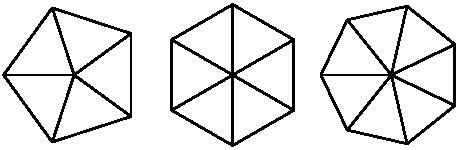
\includegraphics[scale=0.8]{figs/pies.pdf}}
\caption{餅.}
\label{fig.pies}
\end{figure}


\begin{exercise}
\index{pie}

編寫函數, 繪製圖~\ref{fig.pies}中圖形. 

參閱: \url{http://thinkpython2.com/code/pie.py}.

\end{exercise}

\begin{exercise}
\index{alphabet}
\index{turtle typewriter}
\index{typewriter, turtle}

字母表中的字母都是由幾個基礎元素構成, 比如垂直線和水平線, 以及曲線. 
設計個字母表, 使用種類最少的基本元素, 編寫函數繪製字母. 

你要為每個字母開發函數, 比如 \verb"draw_a", \verb"draw_b",等等, 
將這些函數放在名為{\tt letters.py}的文件中. 
你可以從 \url{http://thinkpython2.com/code/typewriter.py}下載個``turtle typewriter'', 
來校驗代碼. 

可參閱 \url{http://thinkpython2.com/code/letters.py};以及
\url{http://thinkpython2.com/code/polygon.py}.

\end{exercise}

\begin{exercise}

去\url{http://en.wikipedia.org/wiki/Spiral}了解一下螺旋線;
然後編碼實現一個阿基米德螺線(或其他種類). 
參閱: \url{http://thinkpython2.com/code/spiral.py}.
\index{spiral}
\index{Archimedian spiral} 

\end{exercise}


\chapter{條件和遞歸}

本章的重點是{\tt if}語句, 
基於程式的狀態不同, 執行不同的代碼. 
但首先我要先介紹兩個新的運算子: 向下取整和求模. 

\section{向下取整和求模}

{\bf 向下取整} 運算子,即 \verb"//", 
兩數相除, 結果向下取整. 
例如, 假設某電影時長105分鐘, 你想知道按小時計, 是多長時間. 
一般除法返回的是浮點數:

\begin{verbatim}
>>> minutes = 105
>>> minutes / 60
1.75
\end{verbatim}

但一般我們表示小時, 不用小數格式. 
向下取整返回的就是整的小時數, 捨棄了小數部分:

\begin{verbatim}
>>> minutes = 105
>>> hours = minutes // 60
>>> hours
1
\end{verbatim}

要想知道捨棄的分鐘數, 只需減去一小時, 剩下的便是了:

\begin{verbatim}
>>> remainder = minutes - hours * 60
>>> remainder
45
\end{verbatim}

\index{floor division}
\index{floating-point division}
\index{division!floor}
\index{division!floating-point}
\index{modulus operator}
\index{operator!modulus}

還可以使用 {\bf 求模運算子},  \verb"%",  
兩數相除, 返回餘數. 

\begin{verbatim}
>>> remainder = minutes % 60
>>> remainder
45
\end{verbatim}
%
求模運算的用途不止於此. 例如, 看一個數字是否可以被另一個整除--如果
{\tt x \% y}結果為0, 則{\tt x}可以被{\tt y}整除.
\index{divisibility}

你也可以通過求模從數字中提取一位或多位餘數. 
例如,  {\tt x \% 10}獲取的便是{\tt x} 除以10後剩下的餘數. 
同樣, {\tt x \% 100}獲取的就是兩位餘數. 

如果你使用的是Python 2, 除法略有不同. 
其除法運算子, \verb"/",  會在兩個整數相除時, 自動向下取整, 
如果有一個是{\tt 浮點數}, 那麼結果才是浮點格式. 
\index{Python 2}


\section{布爾表達式}
\index{boolean expression}
\index{expression!boolean}
\index{logical operator}
\index{operator!logical}

{\bf 布爾表達式} 是用來表示結果是對或錯的表達式. 
下面例子使用運算子{\tt ==},  比較兩個操作數, 
如果相等, 則結果為{\tt True}, 否則為{\tt False}:

\begin{verbatim}
>>> 5 == 5
True
>>> 5 == 6
False
\end{verbatim}
%
{\tt True} 和 {\tt False} 都是{\tt  布爾}格式的值, 不是字符串:
\index{True special value}
\index{False special value}
\index{special value!True}
\index{special value!False}
\index{bool type}
\index{type!bool}

\begin{verbatim}
>>> type(True)
<class 'bool'>
>>> type(False)
<class 'bool'>
\end{verbatim}
%
 {\tt ==}運算子是{\bf 關係運算子}的一種, 其他還有:

\begin{verbatim}
      x != y               # x不等於 y
      x > y                # x 大於 y
      x < y                # x 小於 y
      x >= y               # x 大於等於 y
      x <= y               # x 小於等於 y
\end{verbatim}
%
雖然這些運算子對你來說並不陌生, 但是Python中的運算子和數學裡的不同. 
一個很常見的錯誤就是混淆單等號({\tt =})和雙等號({\tt ==}). 
要知道,  {\tt =}是賦值運算子, 而{\tt ==}是關係運算子. 
而且也沒有{\tt =<} 和 {\tt =>}這種運算子. 
\index{relational operator}
\index{operator!relational}


\section {邏輯運算子}
\index{logical operator}
\index{operator!logical}

有三種{\bf 邏輯運算子}: {\tt and}, {\tt or}, 和 {\tt not}.
其語義和英文中的意思很相似. 例如
{\tt x > 0 and x < 10} 表示只有在 {\tt x} 大於0 {\em 且}小於10時才為真.
\index{and operator}
\index{or operator}
\index{not operator}
\index{operator!and}
\index{operator!or}
\index{operator!not}

{\tt n\%2 == 0 or n\%3 == 0} 需要在{\em 一個或者全部}條件都成立時為真, 
也就是說, 被2整除{\em 或}被3整除. 

最後, {\tt not}運算子是個對布爾表達式取反的操作. 
所以, 當{\tt x > y}為假,  {\tt not (x > y)}便為真, 
也就表示{\tt x}小於或者等於{\tt y}時, 為真.

嚴格來說, 邏輯運算子的操作數都應該是布爾表達式, 不過Python在這方面不太嚴格. 
任何非零的數都當作{\tt True}:

\begin{verbatim}
>>> 42 and True
True
\end{verbatim}
%
這種靈活性固然有用, 但是一些細微差異, 會令人困惑. 
盡量不要如此使用(除非你知道你在做什麼).


\section{條件執行}
\label{conditional.execution}

\index{conditional statement}
\index{statement!conditional}
\index{if statement}
\index{statement!if}
\index{conditional execution}
若想寫出實用性強的程式, 就必然需要程式可以根據條件, 進行選擇處理. 
{\bf 條件語句} 便可以解決此難題. 
最簡單的便是{\tt if} 語句:

\begin{verbatim}
if x > 0:
    print('x is positive')
\end{verbatim}
%
{\tt if}後面的布爾表達式, 叫在{\bf 條件}. 
如果為真, 則縮進的語句執行, 如果為假, 則不執行. 
\index{condition}
\index{compound statement}
\index{statement!compound}

{\tt if} 語句和函數定義的結構一樣: 頭部和緊隨其後的縮進體. 
這樣的語句統稱為{\bf 複合語句}.

縮進體對於語句行數沒有限制, 不過至少要有一行. 
但是有時候, 縮進體暫時不想寫語句(類似於待寫代碼的占位符), 
這種情況, 可以使用 {\tt pass}語句, 表示不做任何操作.
\index{pass statement}
\index{statement!pass}

\begin{verbatim}
if x < 0:
    pass          # TODO:需處理負數!
\end{verbatim}
%

\section{選擇執行}
\label{alternative.execution}
\index{alternative execution}
\index{else keyword}
\index{keyword!else}
{\tt if} 語句第二種使用場景, 便是``選擇執行'',
一般存在兩種選擇, 具體執行哪個, 需要根據條件判斷. 
語義結構如下:

\begin{verbatim}
if x % 2 == 0:
    print('x is even')
else:
    print('x is odd')
\end{verbatim}
%
如果 {\tt x}對2取余後, 結果為0,則{\tt x}為偶數, 並輸出相應信息. 
如果不為0, 則執行第二組語句. 
這種條件非真即假, 必然有相應方案會執行. 這些方案, 叫做{\bf 分支}, 
因為它們屬於執行流程上的分叉. 
\index{branch}



\section{鏈式條件}
\index{chained conditional}
\index{conditional!chained}
有時候, 會遇到多種可能方案, 便需要更多的分支. 
一種方式是採用{\bf 鏈式條件}進行處理:

\begin{verbatim}
if x < y:
    print('x is less than y')
elif x > y:
    print('x is greater than y')
else:
    print('x and y are equal')
\end{verbatim}
%
{\tt elif}  是``else if''的縮寫. 同樣, 上述代碼也只有一個分支會運行. 
對於{\tt elif}語句的數量, 沒有限制. 
至於{\tt else}, 不是必須的, 但如果有的話, 則必須放到結尾.
\index{elif keyword}
\index{keyword!elif}

\begin{verbatim}
if choice == 'a':
    draw_a()
elif choice == 'b':
    draw_b()
elif choice == 'c':
    draw_c()
\end{verbatim}
%
這些條件都是順序檢驗. 如果一個為假, 則檢驗下一個, 依此類推. 
如果條件為真, 則相應分支開始執行, 同時這些判斷語句也都不會再執行. 
即使存在多個條件為真, 那也只會執行第一個為真的分支.  


\section{嵌套條件}
\index{nested conditional}
\index{conditional!nested}

條件判斷也可以嵌套於其他條件內. 
可以將上一節的例子改寫如下:

\begin{verbatim}
if x == y:
    print('x and y are equal')
else:
    if x < y:
        print('x is less than y')
    else:
        print('x is greater than y')
\end{verbatim}
%
外部的條件判斷包含兩個分支. 
第一個只包含一個簡單語句. 
第二個則包含另外一個{\tt if}語句, 
這個語句又包含兩個分支, 這兩個分支也都很簡單, 只是簡單語句. 
同樣, 它們的位置也可以繼續放條件語句.

雖然語句的縮進可以使代碼結構清晰, 但是{\bf 嵌套條件}的語句閱讀起來卻很麻煩. 
所以, 最好還是盡量不用. 

邏輯運算子可以有效簡化嵌套條件語句, 例如, 可以用一行條件語句來重寫下面的代碼:

\begin{verbatim}
if 0 < x:
    if x < 10:
        print('x is a positive single-digit number.')
\end{verbatim}
%
只有兩個條件都滿足, {\tt print} 語句才會運行, 這恰恰和{\tt and}運算子的作用一樣:

\begin{verbatim}
if 0 < x and x < 10:
    print('x is a positive single-digit number.')
\end{verbatim}

對於這種條件判斷, Python提供了更簡潔的方案:

\begin{verbatim}
if 0 < x < 10:
    print('x is a positive single-digit number.')
\end{verbatim}


\section{遞歸}
\label{recursion}
\index{recursion}

既然一個函數可以調用另一個函數, 那麼, 函數也就可以調用自身. 
雖然目前還未看到其用途, 但這卻是程式最神奇的功能之一了. 
看看以下示例:

\begin{verbatim}
def countdown(n):
    if n <= 0:
        print('Blastoff!')
    else:
        print(n)
        countdown(n-1)
\end{verbatim}
%
如果{\tt n} 為0或負數, 輸出單詞 ``Blastoff!''. 
否則, 輸出{ \tt n} , 然後調用函數自身{\tt countdown}並以{\tt n-1}為實參. 

如果如下一般調用此函數, 會如何?

\begin{verbatim}
>>> countdown(3)
\end{verbatim}
%

調用{\tt countdown}, 並且{\tt n=3}, 由於{\tt n}大於0, 輸出3並以{\tt n-1}為參數
調用自身...

\begin{quote}
調用{\tt countdown},  並且{\tt n=2}, 由於{\tt n}大於0, 輸出2並調用自身...

\begin{quote}
調用{\tt countdown},  並且{\tt n=1}, 由於{\tt n}大於0, 輸出1並調用自身...

\begin{quote}
調用{\tt countdown},  並且{\tt n=0}, 由於{\tt n}不大於0, 輸出``Blastoff!'', 
然會返回. 
\end{quote}

{\tt n=1}的 {\tt countdown}執行完結, 返回. 
\end{quote}

{\tt n=2}的 {\tt countdown}執行完結, 返回. 
\end{quote}

{\tt n=3}的 {\tt countdown}執行完結, 返回. 

然後會回到 \verb"__main__"中,  所有輸出如下:
\index{main}

\begin{verbatim}
3
2
1
Blastoff!
\end{verbatim}
%
函數內部調用了自身, 這種函數便是{\bf 可遞歸的};
其執行過程叫做{\bf 遞歸}.
\index{recursion}
\index{function!recursive}

再舉個例子, 我們寫個輸出{\tt n} 次字符串的函數.

\begin{verbatim}
def print_n(s, n):
    if n <= 0:
        return
    print(s)
    print_n(s, n-1)
\end{verbatim}
%
如果{\tt n<=0}, 則 {\bf return 語句}終止函數運行. 
運行流程立刻返回到調用者, 函數其他代碼不執行. 
\index{return statement}
\index{statement!return}

函數其餘部分代碼和{\tt countdown}類似: 
輸出{\tt s},  以 $n-1$ 為參數, 調用自己, 重複$n-1$次. 
那麼, 所有輸出的行數便是 {\tt 1 + (n - 1)},  其和為{\tt n}. 

對於這種簡單樣例, 用{\tt for} 迴圈可能更加方便. 
但是後續我們會遇到一些例子, 用{\tt for}迴圈比較難編寫, 而用遞歸卻輕而易舉, 
所以, 現在不啻為一個好的開始. 
\index{for loop}
\index{loop!for}


\section{遞歸函數堆疊圖}
\label{recursive.stack}
\index{stack diagram}
\index{function frame}
\index{frame}

在第~\ref{stackdiagram}節, 我們使用堆疊圖來描述函數調用時
程式的狀態. 
同樣, 堆疊圖也有助於我們更好理解遞歸函數. 

一旦函數被調用, Python都會創建一個包含函數局部變量以及參數的框. 
所以對於遞歸函數, 可能會同時創建多個框. 

圖~\ref{fig.stack2}便是以{\tt n = 3}為參數, 調用{\tt countdown}所產生的堆疊圖. 

\begin{figure}
\centerline
{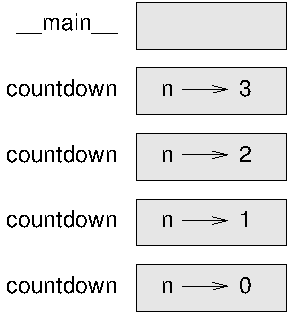
\includegraphics[scale=0.8]{figs/stack2.pdf}}
\caption{堆疊圖.}
\label{fig.stack2}
\end{figure}

通常, 最頂層的框屬於\verb"__main__". 
其為空, 是因為沒有在\verb"__main__"內創建變量或者傳入參數. 
\index{base case}
\index{recursion!base case}

四個{\tt countdown}的框分別對應不同的{\tt n}值, 最底層{\tt n=0}的堆疊, 叫做
{\tt 邊界條件},  也就是不再進行遞歸調用的堆疊, 所以下面也不會再有其他框了. 

做個練習, 以\verb"s = 'Hello'"和{\tt n=2}為參數, 繪製\verb"print_n"調用的堆疊圖. 
然後編寫名為 \verb"do_n" 的函數, 參數為一個函數對象, 和一個數值{\tt n}. 
使其調用{\tt n}次給定的函數. 


\section{無窮遞歸}
\index{infinite recursion}
\index{recursion!infinite}
\index{runtime error}
\index{error!runtime}
\index{traceback}

如果遞歸一直無法觸及邊界條件, 則會一直調用, 永不終止. 
這便叫做{\bf 無窮遞歸}, 出現這種情況, 往往表示情況不妙. 
下面是個無窮遞歸的極簡程式:

\begin{verbatim}
def recurse():
    recurse()
\end{verbatim}
%
多數編程環境中, 無窮遞歸的程式不會一直運行. 
在Python中, 當達到了最大遞歸深度, 便會報錯:
\index{exception!RuntimeError}
\index{RuntimeError}

\begin{verbatim}
  File "<stdin>", line 2, in recurse
  File "<stdin>", line 2, in recurse
  File "<stdin>", line 2, in recurse
                  .   
                  .
                  .
  File "<stdin>", line 2, in recurse
RuntimeError: Maximum recursion depth exceeded
\end{verbatim}
%
這次的追蹤信息比以往的要長一些. 這個錯誤發生時, 堆疊中已經有1000個{\tt 遞歸}框了!

如若不幸遇到無窮遞歸, 最好重新審視一下你的函數, 確保存在不再遞歸調用的邊界條件. 
如果已有邊界條件, 請檢查是否可以保證其被觸達. 


\section{鍵盤輸入}
\index{keyboard input}

到目前為止, 我們編寫的程式,基本都沒有涉及用戶輸入, 它們每次執行都一樣. 

Python提供了內置函數{\tt input},  可以暫停程式運行, 等待用戶鍵入信息. 
當用戶敲擊{\sf  Return} 或 {\sf Enter}鍵時, 程式恢復運行, 
同時\verb"input"將用戶輸入作為字符串返回. 
在Python 2中, 同樣作用的函數叫做\verb"raw_input".
\index{Python 2}
\index{input function}
\index{function!input}

\begin{verbatim}
>>> text = input()
What are you waiting for?
>>> text
'What are you waiting for?'
\end{verbatim}
%
在接收用戶輸入時, 最好給用戶以提示, 使其知曉要輸入的內容. 
 \verb"input" 的參數便是提示信息內容:
\index{prompt}

\begin{verbatim}
>>> name = input('What...is your name?\n')
What...is your name?
Arthur, King of the Britons!
>>> name
'Arthur, King of the Britons!'
\end{verbatim}
%
提示信息末尾的\verb"\n"是個{\bf 換行符},  表示另起一行的特殊字符. 
所以用戶的輸入信息會處於提示信息下面.  
\index{newline}

如果想要一個整數, 那就要將返回值轉為{\tt int}:

\begin{verbatim}
>>> prompt = 'What...is the airspeed velocity of an unladen swallow?\n'
>>> speed = input(prompt)
What...is the airspeed velocity of an unladen swallow?
42
>>> int(speed)
42
\end{verbatim}
%
但如果用戶輸入的不是數字類型的字符串, 那便要報錯了:

\begin{verbatim}
>>> speed = input(prompt)
What...is the airspeed velocity of an unladen swallow?
What do you mean, an African or a European swallow?
>>> int(speed)
ValueError: invalid literal for int() with base 10
\end{verbatim}
%
後續我們會學習如何應對這種錯誤. 
\index{ValueError}
\index{exception!ValueError}


\section{調試}
\label{whitespace}
\index{debugging}
\index{traceback}

當遇到語法異常或者運行時異常, 其報錯信息詳細而充分, 
但會令人無所適從. 一般最有用的也就下面兩部分:

\begin{itemize}

\item 哪種錯誤

\item 發生何處

\end{itemize}

語法錯誤通常容易識別, 但是有些則會誤導我們. 
空格異常通常比較麻煩, 因為空格和製表({\tt Tab})符都看不到, 所以容易被忽視. 
\index{whitespace}

\begin{verbatim}
>>> x = 5
>>>  y = 6
  File "<stdin>", line 1
    y = 6
    ^
IndentationError: unexpected indent
\end{verbatim}
%
此例中, 問題在於, 第二行多了一個空格. 
但是錯誤信息指向 {\tt y}, 便舞蹈了我們. 
通常, 錯誤信息只標識了錯誤發生的位置, 但是問題代碼可能在
此位置之前甚至是前行代碼. 
\index{error!runtime}
\index{runtime error}

運行時錯誤也如此, 假設以分貝為單位, 計算信噪比. 
公式是$SNR_{db} = 10 \log_{10} (P_{signal} / P_{noise})$. 
在Python中, 編碼如下:

\begin{verbatim}
import math
signal_power = 9
noise_power = 10
ratio = signal_power // noise_power
decibels = 10 * math.log10(ratio)
print(decibels)
\end{verbatim}
%
運行代碼, 會遇到報錯:
%
\index{exception!OverflowError}
\index{OverflowError}

\begin{verbatim}
Traceback (most recent call last):
  File "snr.py", line 5, in ?
    decibels = 10 * math.log10(ratio)
ValueError: math domain error
\end{verbatim}
%
錯誤信息顯示, 問題出在第5行, 
但是這行代碼看不出任何問題. 
為了確定具體問題, 可以輸出{\tt ratio}值, 顯示是0.
那問題便出在第4行, 本應用浮點數除法, 卻誤用了整除.
\index{floor division}
\index{division!floor}

對錯誤信息要仔細閱讀, 但也不能完全偏信. 


\section{術語表}

\begin{description}

\item[向下取整(floor division):] 運算子{\tt //}, 將兩數相除, 結果向下(負無窮方向)取整.
  \index{floor division} 
  \index{division!floor}

\item[求模運算子(modulus operator):]  百分號({\tt \%})表示的運算子, 用於整數, 表示兩數相除後的餘數. 
\index{modulus operator}
\index{operator!modulus}

\item[布爾表達式(boolean expression):]  結果為{\tt True} 或 {\tt False}的表達式.
\index{boolean expression}
\index{expression!boolean}

\item[關係運算子(relational operator):] 比較操作數的運算子: 
{\tt ==}, {\tt !=}, {\tt >}, {\tt <}, {\tt >=}, 和 {\tt <=}.

\item[邏輯運算子(logical operator):]  拼接布爾表達式的運算子: 
{\tt and}, {\tt or}, 以及 {\tt not}.

\item[條件語句(conditional statement):]  根據條件, 確定程式運行流程的語句.
\index{conditional statement}
\index{statement!conditional}

\item[條件(condition):] 條件語句中的布爾表達式, 確定分支走向.
\index{condition}

\item[複合語句(compound statement):]  由頭部和縮進體構成的語句, 頭部以冒號(:)結尾, 
縮進體相對頭部需要縮進.
\index{compound statement}

\item[分支(branch):] 條件語句中可選的語句序列中的一種. 
\index{branch}

\item[鏈式條件(chained conditional):] 一系列可選分支構成的條件語句. 
\index{chained conditional}
\index{conditional!chained}

\item[嵌套條件(nested conditional):]  出現在條件語句的分支中的條件語句. 
\index{nested conditional}
\index{conditional!nested}

\item[返回語句(return statement):] 令函數立刻結束並返回給調用方的語句. 
\index{return statement}

\item[遞歸(recursion):]  函數調用自身的過程. 
\index{recursion}

\item[邊界條件(base case):]  遞歸函數中不再進行遞歸調用的條件分支. 
\index{base case}

\item[無窮遞歸(infinite recursion):]  不存在或者永遠無法觸及邊界條件的遞歸, 最終, 無窮遞歸會報運行時異常.
\index{infinite recursion}

\end{description}

\section{習題集}

\begin{exercise}

{\tt time}模塊提供同樣名為{\tt time}的函數, 此函數以某個``時間點''為基準, 
返回當前格林威治時間戳. 理論上, 可以以任意時間為參考點, 而在Unix系統中, 
一般以1970年1月1日為參考``時間點''. 

\begin{verbatim}
>>> import time
>>> time.time()
1437746094.5735958
\end{verbatim}

編寫腳本, 實現將當前時間轉換為一天中的時間(以時分秒為格式), 
以及基準時間點以來的天數. 

\end{exercise}


\begin{exercise}
\index{Fermat's Last Theorem}

費馬大定理說, 沒有任何正整數
$a$, $b$, 和 $c$ 滿足

\[ a^n + b^n = c^n \]
%
當$n$大於2時.

\begin{enumerate}

\item 編寫函數 \verb"check_fermat" , 四個入參---{\tt a}, {\tt b}, {\tt c} 和 {\tt n}---
以檢驗費馬大定理是否成立. 
如果$n$大於2同時滿足

\[a^n + b^n = c^n \]
%
那麼程式應輸出,  ``Holy smokes, Fermat was wrong!'', 
否則, 輸出``No, that doesn't work.''

\item 編寫函數, 令用戶輸入 {\tt a}, {\tt b}, {\tt c} 和 {\tt n}, 
並將其轉換為整數, 然後用\verb"check_fermat" 來檢驗是否違背了費馬大定理. 

\end{enumerate}

\end{exercise}


\begin{exercise}
\index{triangle}

給你三根木棍, 你不一定可以將其拼成三角形, 比如, 一根12英寸長, 
其餘兩根1英寸長, 這兩根太短, 以至於都到不了長的那根的中間. 
所以, 對於三根任意長度的木棍, 有個簡單方案, 可以檢驗其是否可以拼成三角形:

\begin{quotation}
三根木棍中, 如果有任意一根長度大於另外兩根之和, 便拼不成三角形. 
否則, 便可以拼成三角形. (如果兩邊之和等於第三邊, 便稱其為``退化''三角形. )
\end{quotation}

\begin{enumerate}

\item 編寫\verb"is_triangle" 函數, 以三個整數變量為入參, 
同時根據三個特定長度的木棍是否可以拼成三角形, 來輸出 ``Yes'' 或 ``No''. 

\item 編寫函數, 提示用戶輸入三個木棍的長度, 並將其轉換為整數, 
然後用\verb"is_triangle"檢測這三個值是否可以拼成三角形. 
\end{enumerate}

\end{exercise}

\begin{exercise}
下面的程式會輸出什麼?繪製堆疊圖, 展示輸出結果時的程式狀態.

\begin{verbatim}
def recurse(n, s):
    if n == 0:
        print(s)
    else:
        recurse(n-1, n+s)

recurse(3, 0)
\end{verbatim}

\begin{enumerate}

\item 調用 {\tt  recurse(-1, 0)}, 會發生什麼?

\item 為此函數編寫幫助文檔, 告知使用函數所須了解的相關信息(僅此而已).

\end{enumerate}

\end{exercise}

以下練習需要用到第~\ref{turtlechap}節提到的{\tt turtle}模塊:
\index{turtle module}

\begin{exercise}
閱讀下面函數, 看看是否能明白其功能(參閱第~\ref{turtlechap}節的案例). 
運行並看看是否正確. 

\begin{verbatim}
def draw(t, length, n):
    if n == 0:
        return
    angle = 50
    t.fd(length*n)
    t.lt(angle)
    draw(t, length, n-1)
    t.rt(2*angle)
    draw(t, length, n-1)
    t.lt(angle)
    t.bk(length*n)
\end{verbatim}

\end{exercise}


\begin{figure}
\centerline
{
\includegraphics[scale=0.8]{figs/koch.pdf}}
\caption{科赫曲線.}
\label{fig.koch}
\end{figure}

\begin{exercise}
\index{Koch curve}

科赫曲線(The Koch curve) 是類似圖~\ref{fig.koch}的一種分形幾何. 
要想繪製長度為$x$的曲線, 下面是需要做的:

\begin{enumerate}

\item 繪製長為$x/3$的科赫曲線. 

\item 左轉60度. 

\item 繼續繪製長 $x/3$的曲線. 

\item 右轉120度. 

\item 再繪製長 $x/3$的曲線. 

\item 左轉60度. 

\item 繪製長為 $x/3$的曲線. 

\end{enumerate}

當$x$小於3時, 會有所不同:  在此情況下, 繪製所得為長$x$的一段直線. 

\begin{enumerate}

\item 編寫{\tt koch}函數, 以 turtle 和長度length為參數, 使用turtle, 根據指定長度, 繪製
科赫曲線. 

\item 編寫{\tt snowflake}函數, 使其繪製三條科赫曲線, 
從而構成雪花的輪廓.

參閱: \url{http://thinkpython2.com/code/koch.py}.

\item 生成科赫曲線有多種方法. 參看
\url{http://en.wikipedia.org/wiki/Koch_snowflake} 上的案例, 選擇你喜歡的進行實現. 


\end{enumerate}
\end{exercise}


\chapter{有值返回函數}
\label{fruitchap}

目前我們用到的很多Python函數都有返回值, 比如math函數. 
但我們目前寫的函數, 都是無返回值的: 它們只是實現特定的效果, 比如輸出值, 
或者移動小烏龜, 只是它們都沒有返回值. 
本章, 重點學習如何編寫有值返回函數. 

\section{返回值}
\index{return value}

調用函數便會產生返回值, 一般被賦值給變量或者作為表達式的一部分使用. 

\begin{verbatim}
e = math.exp(1.0)
height = radius * math.sin(radians)
\end{verbatim}
%
目前寫的函數, 多是無返回值的. 籠統講, 是沒有返回值, 然而, 
更準確地說, 返回值是空({\tt None}).

本章, 我們總算要寫一些有返回值的函數了. 
第一個例子是 {\tt area}, 根據給定的半徑, 返回面積:

\begin{verbatim}
def area(radius):
    a = math.pi * radius**2
    return a
\end{verbatim}
%
前面我們學過了{\tt return} 語句, 但是在有值返回的函數中, 
{\tt return} 語句包含表達式. 
其意思為:``立即將此表達式作為返回值進行返回. ''
鑑於表達式可簡可繁, 上述函數可以精煉為下面樣子:
\index{return statement}
\index{statement!return}

\begin{verbatim}
def area(radius):
    return math.pi * radius**2
\end{verbatim}
%
但是, 使用類似{\tt a}這樣的{\bf 臨時變量}, 更加清晰明了, 便於調試. 
\index{temporary variable}
\index{variable!temporary}

有時候, 根據條件設置多個不同返回語句, 更加高效:

\begin{verbatim}
def absolute_value(x):
    if x < 0:
        return -x
    else:
        return x
\end{verbatim}
%
這些{\tt return}語句都處於可選條件分支中, 而且, 只有一個會執行. 

一旦返回語句執行, 函數不再執行後續語句, 立刻終止運行. 
{\tt return}語句後的代碼, 或者任何不被觸及的代碼, 都叫做{\bf 無效代碼}.
\index{dead code}

有值返回函數中, 最好保證程式中的每種可能情況, 都有{\tt return}語句. 例如:

\begin{verbatim}
def absolute_value(x):
    if x < 0:
        return -x
    if x > 0:
        return x
\end{verbatim}
%

這個函數錯誤之處在於, 如果{\tt x}恰好是0,
便沒有條件為真, 也就不會觸及任何{\tt return}語句. 
即使運行到函數最後, 返回值也會是{\tt None}, 而不會是0的絕對值. 
\index{None special value}
\index{special value!None}

\begin{verbatim}
>>> print(absolute_value(0))
None
\end{verbatim}
%
順便提一下, Python提供了內置函數{\tt abs}來計算絕對值. 
\index{abs function}
\index{function!abs}

做個練習, 編寫 {\tt compare} 函數, 輸入為{\tt x} 和 {\tt y}, 
如果 {\tt x > y},  返回 {\tt 1}, 
如果{\tt x == y},  返回{\tt 0} , 
如果 {\tt x < y},  返回{\tt -1}. 
\index{compare function}
\index{function!compare}


\section{增量開發}
\label{incremental.development}
\index{development plan!incremental}

隨著編寫的函數越來越長, 你會發現, 調試時間也越來越恐怖. 

若想解決越來越複雜的程式, 可以試試新的方法, 即{\bf 增量開發}.
增量開發是通過每次只編寫並測試少量代碼, 從而避免
長時間的連續開發調試. 
\index{testing!incremental development}
\index{Pythagorean theorem}

比如, 若想計算兩坐標 $(x_1, y_1)$ 和 $(x_2, y_2)$之間的距離, 
根據勾股定理, 可以得到距離為:

\begin{displaymath}
\mathrm{distance} = \sqrt{(x_2 - x_1)^2 + (y_2 - y_1)^2}
\end{displaymath}
%
首先考慮 {\tt distance}函數是什麼樣子. 換句話說, 就是何為輸入(形參), 
何為輸出(返回值)?

此例中, 輸入為兩個點, 即四個值表示的坐標. 返回值為兩點的距離, 用浮點數表示. 

馬上你便可以寫出函數的大致輪廓:

\begin{verbatim}
def distance(x1, y1, x2, y2):
    return 0.0
\end{verbatim}
%
顯然, 此函數無法計算距離, 因為其總是返回0.
但是, 此函數語法正確, 所以可以運行, 
這意味著, 在其變複雜之前, 你能夠對其進行測試. 

用實例參數調用此函數, 看看效果:

\begin{verbatim}
>>> distance(1, 2, 4, 6)
0.0
\end{verbatim}
%
選擇這些值作為坐標, 是因為其水平距離是3,垂直距離是4,兩點距離便是5, 
也就是3-4-5直角三角形的斜邊. 
在測試函數過程中, 知道預期結果, 尤為重要. 
\index{testing!knowing the answer}

我們已經確認此函數語法正確, 現在便可以補充完善代碼了. 
首先, 我們計算$x_2 - x_1$ 和 $y_2 - y_1$的值, 保存為臨時變量, 並輸出. 

\begin{verbatim}
def distance(x1, y1, x2, y2):
    dx = x2 - x1
    dy = y2 - y1
    print('dx is', dx)
    print('dy is', dy)
    return 0.0
\end{verbatim}
%
如果函數正常, 則會輸出\verb"dx is 3" 和 \verb"dy is 4". 
這樣, 我們便知道函數入參正確, 同時前期的計算無誤. 
如果發生異常, 那麼我們只需要仔細檢查這幾行代碼. 

下一步, 計算{\tt dx} 和 {\tt dy}的平方和:

\begin{verbatim}
def distance(x1, y1, x2, y2):
    dx = x2 - x1
    dy = y2 - y1
    dsquared = dx**2 + dy**2
    print('dsquared is: ', dsquared)
    return 0.0
\end{verbatim}
%
再次運行代碼, 並檢查輸出(輸出值應為25). 
最後, 使用 {\tt math.sqrt} 計算最終的返回值:
\index{sqrt}
\index{function!sqrt}

\begin{verbatim}
def distance(x1, y1, x2, y2):
    dx = x2 - x1
    dy = y2 - y1
    dsquared = dx**2 + dy**2
    result = math.sqrt(dsquared)
    return result
\end{verbatim}
%
如果運行正常, 意味著程式正確. 
否則, 就要輸出返回語句前的 {\tt result} 的值, 仔細排查. 

最終版本的函數, 除了返回一個值, 不會輸出任何信息. 
{\tt print} 語句只是為了便於調試代碼, 一旦確認程式無誤, 就應將其移除. 
類似這種代碼, 一般叫做{\bf 腳手架代碼},  主要用來輔助構建程式, 而並不應
忝列最終成品之中. 
\index{scaffolding}

開始時, 一般每次只增加一兩行代碼. 但隨著經驗增長, 慢慢你便可以駕馭大段代碼了. 
無論如何, 增量開發都能節約大量調試時間.

此流程的主要步驟如下:

\begin{enumerate}

\item 首先寫個可運行的程式, 然後逐步增加. 任何時候遇到錯誤, 都要弄清緣由, 盡快解決. 

\item 利用變量保存中間狀態值, 以便展示和檢驗. 

\item 一旦程式運行正常, 便可以移除冗餘代碼, 並精簡繁瑣的語句. 
但是要警惕不要使代碼難以閱讀和理解. 

\end{enumerate}

做個練習, 用增量開發的方式, 寫個函數{\tt hypotenuse}, 
給定直角三角形的兩個直角邊, 返回斜邊長度. 
開發時, 記錄開發流程的各個階段. 
\index{hypotenuse}



\section{組合}
\index{composition}
\index{function composition}

如你所想, 函數可以調用函數. 
例如, 編寫函數, 輸入兩個坐標, 一個是圓心, 一個是圓周上的點, 
計算圓的面積. 

假設圓心坐標為變量{\tt xc} 和
{\tt yc}, 圓周上點的坐標為{\tt xp} 和 {\tt yp}.
首先要計算圓的半徑, 也就是兩點之間的距離. 
便可以借用之前寫過的 {\tt
distance}的函數, 如下:

\begin{verbatim}
radius = distance(xc, yc, xp, yp)
\end{verbatim}
%
下一步便是根據半徑, 計算面積, 借用之前函數:

\begin{verbatim}
result = area(radius)
\end{verbatim}
%
將上述步驟封裝為一個函數, 得到如下:
\index{encapsulation}

\begin{verbatim}
def circle_area(xc, yc, xp, yp):
    radius = distance(xc, yc, xp, yp)
    result = area(radius)
    return result
\end{verbatim}
%
臨時變量{\tt radius} 和 {\tt result} 在開發和調試時有用, 但是程式一旦正常運行, 
便可以通過組合函數調用, 精簡如下:

\begin{verbatim}
def circle_area(xc, yc, xp, yp):
    return area(distance(xc, yc, xp, yp))
\end{verbatim}
%

\section{布爾函數}
\label{boolean}

函數可以返回布爾值, 從而便於隱藏函數內複雜的判斷邏輯.  \index{boolean function}
例如:

\begin{verbatim}
def is_divisible(x, y):
    if x % y == 0:
        return True
    else:
        return False
\end{verbatim}
%
給布爾函數命名, 通常採用類似是/否提問的詞語; 
\verb"is_divisible" 返回 {\tt True} 或 {\tt False}, 
以表明{\tt x}是否被{\tt y}整除. 
比如:

\begin{verbatim}
>>> is_divisible(6, 4)
False
>>> is_divisible(6, 3)
True
\end{verbatim}
%
 既然{\tt ==}運算子的結果為布爾值, 
我們便可以直接返回, 從而精簡函數:

\begin{verbatim}
def is_divisible(x, y):
    return x % y == 0
\end{verbatim}
%
布爾函數一般用於條件語句:
\index{conditional statement}
\index{statement!conditional}

\begin{verbatim}
if is_divisible(x, y):
    print('x is divisible by y')
\end{verbatim}
%
也可以這麼寫:

\begin{verbatim}
if is_divisible(x, y) == True:
    print('x is divisible by y')
\end{verbatim}
%
但這個比較就顯得多餘了. 

做個練習, 編寫函數 \verb"is_between(x, y, z)", 
如果$x \le y \le z$, 返回{\tt True}, 否則返回{\tt False}.


\section{再說遞歸}
\label{more.recursion}
\index{recursion}
\index{Turing complete language}
\index{language!Turing complete}
\index{Turing, Alan}
\index{Turing Thesis}

目前, 我們只學到了Python的一小部分, 但麻雀雖小, 五臟俱全, 
這一小部分便足以表達一門{\em 完整的}編程語言了, 
也就是說, 如果一切皆是計算, 那麼以上所學便已足夠. 
任何程式都可以只用以上所學模塊, 進行構建(當然, 可能還需要一些控制設備
的命令, 比如管理鼠標, 硬盤等, 但是也僅需要這些).

最早證明了上述偉大結論的是艾蘭圖靈(Alan Turing), 最早的電腦科學家之一
(有人會計較其是數學家, 但是早期的電腦科學家, 基本都是數學家). 
因此, 這個理論也叫做圖靈論斷(Turing Thesis). 
關於圖靈論斷, 如果想更加詳細深入了解, 我推薦 Michael Sipser 所寫
 {\em 計算理論導引(Introduction to the Theory of Computation)} 一書.

為了展示目前所學的威力, 我們分析幾個遞歸數學函數. 
遞歸定義和迴圈定義類似, 某種意義上說, 函數定義體內包含了對定義體的引用. 
通常一個完全迴圈的定義, 是無用的:

\begin{description}

\item[致命的:] 一個形容詞, 用來描述一些致命的東西.
\index{vorpal}
\index{circular definition}
\index{definition!circular}

\end{description}

如果在辭典中看到這樣的定義, 一定鬱悶. 
但你如果查詢一下用符號$!$表示的階乘運算, 
會看到以下內容:
%
\begin{eqnarray*}
&&  0! = 1 \\
&&  n! = n (n-1)!
\end{eqnarray*}
%
這個定義聲明0的階乘為1, 同時對於任意$n$值的階乘, 便是$n$乘以$n-1$的階乘. 

所以$3!$表示3乘以$2!$,  而$2!$表示2乘以$1!$, $1!$又是1乘以
$0!$. 整理一下, $3!$ 等於3乘以2乘以1再乘以1,也就是6.
\index{factorial function}
\index{function!factorial}
\index{recursive definition}

如果你可以編寫其遞歸定義, 那便可以編寫Python實現它. 
首先要確定參數. 很顯然, 此處{\tt factorial}函數的參數為整數:

\begin{verbatim}
def factorial(n):
\end{verbatim}
%
如果參數恰好為0, 只需要返回1:

\begin{verbatim}
def factorial(n):
    if n == 0:
        return 1
\end{verbatim}
%
而其他情況就有意思了, 需要遞歸調用以找到$n-1$的階乘, 然後將其與
$n$相乘:

\begin{verbatim}
def factorial(n):
    if n == 0:
        return 1
    else:
        recurse = factorial(n-1)
        result = n * recurse
        return result
\end{verbatim}
%
此程式的執行流程和第~\ref{recursion}節的{\tt
countdown}極為相似. 如果以3為參數調用{\tt factorial}:

3不等於0,則走第二分支, 計算{\tt n-1}的階乘...

\begin{quote}
2不等於0,則走第二分支, 計算{\tt n-1}的階乘...


  \begin{quote}
 1不等於0,則走第二分支, 計算{\tt n-1}的階乘...


    \begin{quote}
   0等於0, 則走第一分支, 不再遞歸調用, 返回1.
    \end{quote}

  返回值1乘以$n$, 而$n$此時為1,則返回1. 
  \end{quote}

返回值1乘以$n$, 此時$n$為2, 返回為2的結果.
\end{quote}

返回值(2)乘以此時為3的$n$, 結果為6, 也就是整個流程最終的結果. 
\index{stack diagram}

圖~\ref{fig.stack3} 是這一系列函數調用的堆疊圖展現.

\begin{figure}
\centerline
{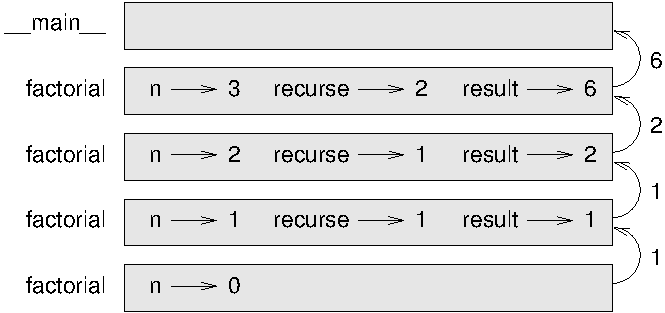
\includegraphics[scale=0.8]{figs/stack3.pdf}}
\caption{堆疊圖.}
\label{fig.stack3}
\end{figure}

返回值會在堆疊中被傳遞. 
每個框內, 返回值就是{\tt result}的值, 也就是{\tt recurse}和{\tt n}相乘的結果. 
\index{function frame}
\index{frame}

最後的框中, 沒有局部變量{\tt recurse}和{\tt result} , 是因為
沒有走第二分支. 

\section{置信遷移}
\index{recursion}
\index{leap of faith}

閱讀程式的一種方式是跟蹤其執行順序, 但是你很快會不堪重負. 
另一種可行方案, 我稱之為``置信遷移''. 當遇到某個函數調用時, 
不是根據執行流程深入跟蹤, 
而是{\em 假設}這個函數工作正常, 可以返回正確結果. 

實際你在使用內置函數時, 就在實踐置信遷移了. 調用
{\tt math.cos} 或 {\tt math.exp}時, 並沒有深入檢查其函數執行體. 
這是因為你相信寫出這些內置函數的人是優秀的編程人員, 
所以相信這些函數可以正確運行. 

對於你來說, 調用自己的函數也是同理. 例如第~\ref{boolean}節, 
我們編寫了\verb"is_divisible"函數, 用來判斷一個數是否可以被另一個數
整除. 如果我們自己相信這些函數是正確的--分析代碼並測試都通過--
我們便可以直接使用它, 而無需再探究細節. 
\index{testing!leap of faith}

遞歸程式也一樣. 當你進行遞歸調用時, 
無需一步步跟蹤運行流程, 你應該相信遞歸調用運行正常
(會返回正確的結果), 然後問問自己, ``既然我可以計算出 $n-1$的階乘, 那麼
是不是我也可以計算出$n$的階乘?" 很顯然你可以, 乘以$n$即可. 

當然, 沒有完成函數編寫, 便假設其正常運行, 是有點奇怪, 
所以這也是我們稱其為置信遷移的原因!


\section{另例}
\label{one.more.example}

\index{fibonacci function}
\index{function!fibonacci}
在了解{\tt 階乘}之後, 我們要學習的是遞歸數學函數中最常見的用例, 
{\tt 斐波拉契數列}. 
其詳細定義可參閱\url{http://en.wikipedia.org/wiki/Fibonacci_number}:
%
\begin{eqnarray*}
&& \mathrm{fibonacci}(0) = 0 \\
&& \mathrm{fibonacci}(1) = 1 \\
&& \mathrm{fibonacci}(n) = \mathrm{fibonacci}(n-1) + \mathrm{fibonacci}(n-2)
\end{eqnarray*}
%
翻譯為Python代碼, 代碼如下:

\begin{verbatim}
def fibonacci(n):
    if n == 0:
        return 0
    elif  n == 1:
        return 1
    else:
        return fibonacci(n-1) + fibonacci(n-2)
\end{verbatim}
%
若你嘗試跟蹤其流轉, 那即使一個很小的$n$值, 都能令你頭疼. 
但是, 基於置信遷移, 如果兩個遞歸調用都運行正常, 那麼很顯然, 
將其相加, 便能得到正確結果. 
\index{flow of execution}


\section{類型檢查}
\label{guardian}

試試給 {\tt factorial}函數傳遞個1.5的參數, 會發生什麼?
\index{type checking}
\index{error checking}
\index{factorial function}
\index{RuntimeError}

\begin{verbatim}
>>> factorial(1.5)
RuntimeError: Maximum recursion depth exceeded
\end{verbatim}
%
看起來陷入了無窮遞歸. 怎麼會這樣? 此函數有個邊界條件--當 {\tt n == 0}時. 
但如果{\tt n}不是整數, 那便會{\em 掠過} 邊界條件, 一直遞歸下去. 
\index{infinite recursion}
\index{recursion!infinite}

第一次遞歸調用中, { \tt n}是0.5. 
下一次, 變成了-0.5.再然後, 會越來越小(更小的負數), 
也就永遠不可能再成為0.

我們有兩種方案. 一種是嘗試改進{\tt factorial}函數, 使其支持浮點數, 
或者使其檢驗參數類型. 
第一種方案會寫出伽瑪函數, 超出了本書的範疇. 所以選擇方案二. 
\index{gamma function}

我們可以使用內置 {\tt isinstance} 函數來檢驗參數類型. 
同時, 我們也需要保證參數是正數:
\index{isinstance function}
\index{function!isinstance}

\begin{verbatim}
def factorial(n):
    if not isinstance(n, int):
        print('Factorial is only defined for integers.')
        return None
    elif n < 0:
        print('Factorial is not defined for negative integers.')
        return None
    elif n == 0:
        return 1
    else:
        return n * factorial(n-1)
\end{verbatim}
%
第一個邊界條件, 針對非整數;
第二個, 則針對負整數. 
這兩個邊界條件中, 都會輸出錯誤信息, 並返回{\tt None}, 
以標識運行錯誤:

\begin{verbatim}
>>> print(factorial('fred'))
Factorial is only defined for integers.
None
>>> print(factorial(-2))
Factorial is not defined for negative integers.
None
\end{verbatim}
% 
如果通過兩個檢驗, 那可以確定$n$現在是非負整數, 
至此便可以確保遞歸會終止了. 
\index{guardian pattern}
\index{pattern!guardian}

此程式展示了一種叫做{\bf 哨兵}的角色. 
前兩個條件, 就像哨兵一樣, 避免程式犯錯, 使其正確運行. 

在第~\ref{raise}節, 我們會看到一種更靈活的方案來輸出錯誤信息: 上報異常. 


\section{調試}
\label{factdebug}
將程式大而化小, 也就天然地為調試創造了一個個的檢查點. 
如果程式運行異常, 需要考慮以下三種可能原因:
\index{debugging} 

\begin{itemize}

\item 函數入參異常, 前置條件未滿足. 

\item 函數本身異常, 後置條件不滿足. 

\item 返回值或者調用方式異常. 

\end{itemize}

若要避免第一種異常, 可以在函數開始用{\tt  print}語句, 打印參數值(以及類型). 
或者編寫代碼, 校驗前置條件. 
\index{precondition}
\index{postcondition}

如果參數沒問題, 那在每個{\tt return}語句前, 增加{\tt print}語句, 打印返回值. 
如果可以的話, 最好親自檢查結果. 同時盡量在調用函數時, 傳入合適的參數, 
以使返回結果便於校驗
(如第~\ref{incremental.development}節). 

如果函數都正常, 那檢驗一下函數調用方式, 看看是否正確使用了返回值
(或者至少用到了返回值!)
\index{flow of execution}

在函數開頭和結尾添加打印語句, 有助於更直觀地觀察運行流程. 例如, 下面是
包括打印語句的{\tt factorial}版本:

\begin{verbatim}
def factorial(n):
    space = ' ' * (4 * n)
    print(space, 'factorial', n)
    if n == 0:
        print(space, 'returning 1')
        return 1
    else:
        recurse = factorial(n-1)
        result = n * recurse
        print(space, 'returning', result)
        return result
\end{verbatim}
%
在此, 用{\tt 空格}字符串來控制輸出語句的縮進. 以下為{\tt factorial(4)}的運行結果:

\begin{verbatim}
                 factorial 4
             factorial 3
         factorial 2
     factorial 1
 factorial 0
 returning 1
     returning 1
         returning 2
             returning 6
                 returning 24
\end{verbatim}
%
若惑於其函數執行流程, 那麼, 此輸出相比有助於理解. 
有時候, 增加腳手架需要耗費一點時間, 
但是, 這一點時間的花費, 往往能夠節約大量的調試時間. 

\section{術語表}

\begin{description}

\item[臨時變量(temporary variable):] 複雜運算中, 暫存中間值的變量. 
\index{temporary variable}
\index{variable!temporary}

\item[無效代碼(dead code):]  程式永遠不會運行的語句, 通常在{\tt return}語句之後. 
\index{dead code}

\item[增量開發(incremental development):]  一次僅僅開發並測試少量代碼的開發方案, 
小步慢跑, 從而防止費時調試. 
\index{incremental development}

\item[腳手架(scaffolding):]  程式開發中起輔助作用的代碼, 但不會留在最終程式中. 
\index{scaffolding}

\item[哨兵(guardian):]  一種編程模式, 使用條件語句進行檢驗, 並處理可能導致異常的情形. 
\index{guardian pattern}
\index{pattern!guardian}

\end{description}


\section{習題集}

\begin{exercise}
針對以下代碼, 繪製堆疊圖, 查看程式輸出為何?
\index{stack diagram}

\begin{verbatim}
def b(z):
    prod = a(z, z)
    print(z, prod)
    return prod

def a(x, y):
    x = x + 1
    return x * y

def c(x, y, z):
    total = x + y + z
    square = b(total)**2
    return square

x = 1
y = x + 1
print(c(x, y+3, x+y))
\end{verbatim}

\end{exercise}


\begin{exercise}
\label{ackermann}

阿克曼(Ackermann)函數 $A(m, n)$定義如下:

\begin{eqnarray*}
A(m, n) = \begin{cases} 
              n+1 & \mbox{if } m = 0 \\ 
        A(m-1, 1) & \mbox{if } m > 0 \mbox{ and } n = 0 \\ 
A(m-1, A(m, n-1)) & \mbox{if } m > 0 \mbox{ and } n > 0.
\end{cases} 
\end{eqnarray*}
%
參考 \url{http://en.wikipedia.org/wiki/Ackermann_function}.
編寫{\tt ack}函數代碼, 實現Ackermann函數. 
用此代碼執行 {\tt ack(3, 4)}, 結果應該為125. 
同時, 換較大的{\tt m} 和{\tt n}, 看看結果有何不同?
答案參見: \url{http://thinkpython2.com/code/ackermann.py}.
\index{Ackermann function}
\index{function!ack}

\end{exercise}


\begin{exercise}
\label{palindrome}

像``noon''和``redivider''一樣, 正序和倒序拼寫方式完全一樣的詞, 稱為回文詞. 
從遞歸角度看, 如果開始和結束字母相同, 同時中間部分是回文詞, 那麼就可以認為
總體是回文詞. 
\index{palindrome}
下文為返回字符串首字母, 尾字母以及中間字母的函數:

\begin{verbatim}
def first(word):
    return word[0]

def last(word):
    return word[-1]

def middle(word):
    return word[1:-1]
\end{verbatim}
%

在第~\ref{strings}節會詳細解釋其原理.

\begin{enumerate}

\item 將這些函數代碼, 寫入文件{\tt palindrome.py}, 並測試輸出. 
用兩個字母, 測試 {\tt middle} 函數, 看看會怎麼樣? 一個字母呢?  
嘗試傳入不包含任何字母的空字符串\verb"''",  會如何?

\item 編寫\verb"is_palindrome"函數, 如果傳入參數為回文字符串, 
則返回{\tt True},  否則返回{\tt False}. 
提示一下, 你可以使用內置函數{\tt len}檢驗字符串長度. 

\end{enumerate}

答案參閱: \url{http://thinkpython2.com/code/palindrome_soln.py}.

\end{exercise}

\begin{exercise}

如果$a$可以被$b$整除, 同時$a/b$也是$b$的冪次方, 那麼$a$便是$b$是冪次方. 
編寫函數\verb"is_power", 
以 {\tt a} 和 {\tt b}為參數, 如果{\tt a}是{\tt b}的冪次放, 則返回{\tt True}. 
提示:注意邊界條件. 

\end{exercise}


\begin{exercise}
\index{greatest common divisor (GCD)}
\index{GCD (greatest common divisor)}

 $a$ 和 $b$ 的最大公約數(GCD), 是指能同時被整除的所有約數中的最大
的一個. 

尋找最大公約數的一種方法便是觀察, 如果$r$ 是$a$除以$b$的餘數, 
那麼$gcd(a, b) = gcd(b, r)$, 邊界條件是$gcd(a, 0) = a$.

編寫函數\verb"gcd", 以{\tt a} 和 {\tt b}為參數, 返回其最大公約數. 


致謝: 此習題借鑑了 Abelson 和
Sussman 的 {\em Structure and Interpretation of Computer Programs} 中的樣例.

\end{exercise}


\chapter{疊代}

本章主講疊代, 其主要實現重複執行一段語句. 
在第~\ref{recursion}節的遞歸, 便是一種疊代. 
在第~\ref{repetition}節的{\tt for}迴圈, 也是一種疊代. 
本章, 我們會接觸另一種疊代, {\tt while} 語句. 
但這裡要先講一下變量賦值. 

\section{重新賦值}
\index{assignment}
\index{statement!assignment}
\index{reassignment}

你也許已經注意到, 相同的變量可以被多次賦值. 
重新賦值會將已存在的變量指向新的值(並且不再指向舊的值).

\begin{verbatim}
>>> x = 5
>>> x
5
>>> x = 7
>>> x
7
\end{verbatim}
%
第一次輸出{ \tt x}, 值為5, 第二次輸出, 值為7.

圖~\ref{fig.assign2}  展示了堆疊圖中{\bf 重新賦值}
的過程. \index{state diagram} \index{diagram!state}

在此, 我想澄清一下大家的困惑.
因為Python使用等號({\tt =})進行賦值, 
很容易將{\tt a = b}這樣的語句, 作為數學命題中的等式進行解讀, 
認為其表示{\tt a}和{\tt b}相等. 
這種解讀是極其錯誤的. 
\index{equality and assignment}

首先, 等式是對稱關係, 而賦值不是. 
例如, 數學中, 如果 $a=7$, 那麼$7=a$.但是在Python中, 
{\tt a = 7}正確, 但是 {\tt 7 = a}則不然. 

同樣, 在數學領域, 等式結果要麼真要麼假. 
如果$a=b$, 那麼 $a$總是等於$b$. 
而在Python中, 雖然賦值語句可以使兩變量相等, 但是無法保證其一直相等:

\begin{verbatim}
>>> a = 5
>>> b = a    # a 和 b 相等
>>> a = 3    # a 和 b 不等
>>> b
5
\end{verbatim}
%
第三行代碼, 改變了{\tt a}的值, 但是沒有改變{\tt b}, 所以他們不再相等. 

很多時候我們需要給變量重新賦值, 但是要謹慎使用. 
如果變量的值變動過於頻繁, 代碼後續將難以理解, 同時調試困難. 

\begin{figure}
\centerline
{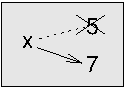
\includegraphics[scale=0.8]{figs/assign2.pdf}}
\caption{堆疊圖}
\label{fig.assign2}
\end{figure}



\section{變量更新}
\label{update}

\index{update}
\index{variable!updating}

最常見的一種重新賦值, 便是{\bf 變量更新},
通常是基於前值進行修改而得到新值. 

\begin{verbatim}
>>> x = x + 1
\end{verbatim}
%
這句代碼表示``獲取{\tt x}的值, 然後加一, 得到新值, 繼而用新值更新{\tt x}.'' 

如果你嘗試更新未定義變量, 會遇到錯誤, 
因為Python會在賦值{\tt x} 前執行右側表達式:

\begin{verbatim}
>>> x = x + 1
NameError: name 'x' is not defined
\end{verbatim}
%
更新變量前, 一定要{\bf 初始化}, 通常採用簡單賦值來實現:
\index{initialization (before update)}

\begin{verbatim}
>>> x = 0
>>> x = x + 1
\end{verbatim}
%
對變量進行加1來使其更新, 叫做{\bf 自增};
執行減1更新變量, 叫做{\bf 自減}. 
\index{increment}
\index{decrement}


\section{{\tt while}語句}
\index{statement!while}
\index{while loop}
\index{loop!while}
\index{iteration}
計算機通常用於自動化一些重複性工作. 
對於大量重複的相同或相似任務, 計算機可以永不犯錯, 
這也是計算機精擅之處, 卻恰恰是人類最不擅長的. 
在計算機編程中, 這種重複, 便稱作{\bf 疊代}.

我們已經遇到過兩個函數,  {\tt countdown} 和
\verb"print_n",  它們都是使用遞歸進行疊代. 
因疊代操作很普遍, Python提供了一些內置功能來便捷使用. 
一個便是在第~\ref{repetition}節見到的{\tt for}語句, 後續再講. 

另一個便是{\tt while}語句, 下面是{\tt
countdown}的 {\tt while}語句版本:

\begin{verbatim}
def countdown(n):
    while n > 0:
        print(n)
        n = n - 1
    print('Blastoff!')
\end{verbatim}
%
{\tt while}語句很容易理解, 因為其便如英語表達一樣. 
意為, ``當{\tt n}大於0時, 打印{\tt n}值, 然後自減1.
直到當等於0時, 打印 {\tt Blastoff!}''
\index{flow of execution}

正式些講, 下面是{\tt while}語句的執行流程:

\begin{enumerate}

\item 確定條件之真假.

\item 如果為假, 退出{\tt while}語句, 執行其後語句. 

\item 如果為真, 運行執行體, 回到第一步. 

\end{enumerate}

這種程式流轉, 便叫做迴圈. 因為第三步驟時, 會返回到起點. 
\index{condition}
\index{loop}
\index{body}

迴圈體通常會修改一個或多個變量的值, 從而令條件最終為假, 終止迴圈. 
否則, 迴圈會一直重複, 成為{\bf 無限迴圈}. 
對電腦科學家們, 有個樂此不疲的玩笑, 
便是觀察洗髮水的使用說明, 
``起泡, 沖洗, 重複'',  這就是個無限迴圈. 
\index{infinite loop}
\index{loop!infinite}

在{\tt countdown}例子中, 我們如此保證迴圈終止:
如果{\tt n}小於或等於0,迴圈不再運行. 
由於{\tt n}每迴圈一次, 就會變小, 終究會變成0.

而有些迴圈, 則不太容易判斷, 比如:

\begin{verbatim}
def sequence(n):
    while n != 1:
        print(n)
        if n % 2 == 0:        # n 是偶數
            n = n / 2
        else:                 # n 是奇數
            n = n*3 + 1
\end{verbatim}
%
此迴圈的條件是{\tt n != 1},  那麼只有{\tt n}等於{\tt 1}時, 條件為假, 迴圈才終止. 

每次迴圈, 程式都輸出{\tt n}的值, 然後檢查是奇是偶. 
如果是偶數, 則{\tt n}除以2. 如果是奇數, 則{\tt n}值更新為{\tt n*3 + 1}. 
例如, 如果{\tt sequence}的參數為3, {\tt n}值依次變為3, 10, 5, 16, 8, 4, 2, 1.


由於{\tt n} 有時增加, 有時減少, 所以很難保證{\tt n}會達到1, 或者程式終止. 
對於某些特殊的{\tt n}值, 我們可以確信迴圈會終止. 
比如, 如果起始值是2的冪, 那麼迴圈每次執行後{\tt n}都會是偶數, 直到最終成為1.
剛剛例子中得到的數列, 從16開始, 便是如此. 
\index{Collatz conjecture}

問題的難點在於, 是否可以證明對於{\em 所有}正數的{\tt n}, 程式都會結束. 
目前, 還沒有人能證明或者證否此命題! 
(參閱 \url{http://en.wikipedia.org/wiki/Collatz_conjecture})

做個練習, 用疊代替換遞歸, 重寫第~\ref{recursion}節的\verb"print_n"函數, 

\section{{\tt break}語句}
\index{break statement}
\index{statement!break}
有時, 想要出紅塵, 就需要先入紅塵, 只有進入迴圈體, 
才知道何時應當終止迴圈. 
這時, 我們可以用{\tt break}語句跳出迴圈. 

例如, 想要獲取用戶的輸入, 直到用戶輸入{\tt done}, 才跳出迴圈, 可以這樣寫:

\begin{verbatim}
while True:
    line = input('> ')
    if line == 'done':
        break
    print(line)

print('Done!')
\end{verbatim}
%
迴圈條件為{\tt True}, 便會一直迴圈, 所以只有觸及 break 語句, 才會跳出迴圈. 

每次迴圈, 都會打印尖括號來提示用戶輸入, 
如果用戶輸入了{\tt done}, {\tt break} 語句會終止迴圈. 
否則, 程式會打印用戶的輸入, 並進入下一輪迴圈. 
舉個例子:

\begin{verbatim}
> not done
not done
> done
Done!
\end{verbatim}
%
這種寫法在{\tt while}迴圈中很常見, 
因為你能夠隨時檢驗其條件(而不僅僅在頭部驗證), 
同時也可以主動地去終止迴圈(``發生時停止''), 
而不是被動地等待結束(``執行到停止'').


\section{平方根}
\label{squareroot}
\index{square root}

在編程中, 迴圈通常用來進行數值計算, 通過用近似值逼近真實值來實現. 
\index{Newton's method}

例如, 牛頓公式(Newton's method)便是一種計算平方根的方法. 
若要計算$a$的平方根, 可以先確定一個任意的估計值, $x$, 
然後通過下面公式, 可以得到一個更優的值:

\[ y = \frac{x + a/x}{2} \]
%
比如, 如果$a$為 4, 且$x$為 3:

\begin{verbatim}
>>> a = 4
>>> x = 3
>>> y = (x + a/x) / 2
>>> y
2.16666666667
\end{verbatim}
%
結果很接近正確答案($\sqrt{4} = 2$).
如果我們用得到的近似值, 重複剛才的流程, 結果會更接近:

\begin{verbatim}
>>> x = y
>>> y = (x + a/x) / 2
>>> y
2.00641025641
\end{verbatim}
%
多重複幾次, 結果便更準確:
\index{update}

\begin{verbatim}
>>> x = y
>>> y = (x + a/x) / 2
>>> y
2.00001024003
>>> x = y
>>> y = (x + a/x) / 2
>>> y
2.00000000003
\end{verbatim}
%
通常, 我們很難預知, 重複多少次, 才能得到正確結果. 
但是, 我們知道, 一旦結果不再改變, 便是停止的時候:

\begin{verbatim}
>>> x = y
>>> y = (x + a/x) / 2
>>> y
2.0
>>> x = y
>>> y = (x + a/x) / 2
>>> y
2.0
\end{verbatim}
%
當{\tt y == x}時, 我們便可以停止迴圈了. 
下面的迴圈, 以估計值{\tt x}開始並不斷逼近真實值, 在結果不再變化時終止:

\begin{verbatim}
while True:
    print(x)
    y = (x + a/x) / 2
    if y == x:
        break
    x = y
\end{verbatim}
%
對於大部分的{\tt a} 值, 此方法都有效. 
但涉及到{\tt 浮點數}等式, 便很麻煩. 
浮點值一般認為是近似正確:
大部分的有理數, 比如$1/3$, 
以及類似$\sqrt{2}$的無理數, 都無法用{\tt 浮點數}來精確表示. 
\index{floating-point}
\index{epsilon}

與其費勁比較 {\tt x} 和 {\tt y} 是否相等, 不如用{\tt abs}計算
其差值的絕對值大小:

\begin{verbatim}
    if abs(y-x) < epsilon:
        break
\end{verbatim}
%
在\verb"epsilon" 為{\tt 0.0000001}時, 表達式為真, 
那便說明兩個值已經足夠接近. 


\section{算法}
\index{algorithm}
牛頓公式可以認為是一種{\bf 算法}:
通過既定步驟來解決一類問題(此例中為計算平方根). 

要理解何為算法, 先要明白什麼不屬於算法. 
當你學習乘法時, 往往需要記憶乘法表. 
實際, 你記憶了100個特定答案. 這種知識不屬於算法. 

但如果你想``偷懶'', 你可能會發現一些小技巧. 
比如, 你想計算$n$和9的乘積, 只需把$n-1$, 作為第一個數字. 
$10-n$作為第二個數字即可. 這個小技巧對於任何數字乘以9都有效. 
這便是算法!
\index{addition with carrying}
\index{carrying, addition with}
\index{subtraction!with borrowing}
\index{borrowing, subtraction with}
同樣地, 你學過的需進位的加法, 需借位的減法, 以及長除法, 
都是算法. 這些算法的一個共性便是, 都無需費力思考. 
它們都是機械的過程, 
遵循簡單的規則, 一步步操作, 便可得到結果. 

執行算法固然無聊, 但其設計過程卻既有趣又挑戰智力, 
同時也是電腦科學的核心. 

有些事情, 對於人們來說很自然, 無難度, 且下意識便可完成, 
而算法卻很難解決. 
比如, 理解自然語言. 我們所有人都能輕易做到, 
但目前為止, 還沒有人能闡明我們是{\em 如何}理解的, 
更不用說用算法的形式來解釋. 

\section{調試}
\label{bisectbug}
隨著程式代碼規模的增長, 你會發現需要耗費更多時間在
調試上. 一般更多的代碼, 也就意味著更多的出錯機會, 
以及更多的潛在問題. 
\index{debugging!by bisection}
\index{bisection, debugging by}
一種有效節約調試時間的方法便是``二分調試''.
比如, 有100行代碼, 一次檢查一行, 需要100次. 

或者, 將程式對半切分. 找到程式的中間位置, 或者靠近中間的位置, 
以便從中間開始檢查. 添加{\tt print}語句(或者其他可驗證效果的東西), 
然後運行代碼. 

如果中間檢查點出現異常, 那代碼前半部分有問題. 
如果中間沒有出錯, 那麼問題便在後半部分了. 

每次如此檢驗代碼, 將待檢驗的代碼行數不斷減半. 大約六步之後(遠遠小於100), 
理論上, 便只剩下一兩行代碼需要檢查了. 

實際上, 很難清晰界定``代碼中間位置'', 同時也很難在其位置檢驗. 
所以沒必要計較於行數, 執著於中點. 
反而, 你需要多思考代碼的哪些位置容易出錯, 哪些地方又容易驗證. 
然後選擇一個恰到好處的點, 進行驗證. 



\section{術語表}

\begin{description}

\item[重新賦值(reassignment):] 給已存在的變量賦新值的過程. 
\index{reassignment}

\item[變量更新(update):] 基於前值, 計算新值, 更新變量的過程. 
\index{update}

\item[初始化(initialization):] 給變量賦初始值, 以待後續更新. 
\index{initialization!variable}

\item[自增(increment):] 不斷增加某個值的變量更新(通常為1). 
\index{increment}

\item[自減(decrement):] 不斷減少某個值的變量更新. 
\index{decrement}

\item[疊代(iteration):] 採用遞歸或者迴圈, 重複執行一段語句. 
\index{iteration}

\item[無限迴圈(infinite loop):] 終止條件一直不能抵達的迴圈. 
\index{infinite loop}

\item[算法(algorithm):]  解決一類問題的通用步驟. 
\index{algorithm}

\end{description}


\section{習題集}

\begin{exercise}
\index{algorithm!square root}

複製第~\ref{squareroot}節的迴圈, 封裝為\verb"mysqrt" 函數, 
令其以{\tt a}為參數, 選擇一個合適的值{\tt x}, 返回{\tt a}的
近似平方根.  \index{encapsulation}

若要測試, 需要編寫一個名為\verb"test_square_root"的函數, 
輸出下面的表格:

\begin{verbatim}
a   mysqrt(a)     math.sqrt(a)  diff
-   ---------     ------------  ----
1.0 1.0           1.0           0.0
2.0 1.41421356237 1.41421356237 2.22044604925e-16
3.0 1.73205080757 1.73205080757 0.0
4.0 2.0           2.0           0.0
5.0 2.2360679775  2.2360679775  0.0
6.0 2.44948974278 2.44948974278 0.0
7.0 2.64575131106 2.64575131106 0.0
8.0 2.82842712475 2.82842712475 4.4408920985e-16
9.0 3.0           3.0           0.0
\end{verbatim}
%
第一列是數值$a$; 第二列是 \verb"mysqrt"函數計算出的$a$的平方根;
第三列是通過{\tt math.sqrt}計算出的平方根;
第四列是兩者的差值絕對值. 
\end{exercise}


\begin{exercise}
\index{eval function}
\index{function!eval}
內置函數 {\tt eval} 以字符串為輸入, 並用Python解釋器執行. 
如下:

\begin{verbatim}
>>> eval('1 + 2 * 3')
7
>>> import math
>>> eval('math.sqrt(5)')
2.2360679774997898
>>> eval('type(math.pi)')
<class 'float'>
\end{verbatim}
%
編寫函數\verb"eval_loop", 不停提示用戶, 獲取輸入並用{\tt eval}執行, 
同時打印結果. 

直到用戶輸入 \verb"'done'"才終止, 
同時返回最後一次表達式的結果. 

\end{exercise}


\begin{exercise}
\index{Ramanujan, Srinivasa}
數學家Srinivasa Ramanujan發現了一個無窮級數, 
可以用來計算$1 / \pi$的近似值:
\index{pi}

\[ \frac{1}{\pi} = \frac{2\sqrt{2}}{9801} 
\sum^\infty_{k=0} \frac{(4k)!(1103+26390k)}{(k!)^4 396^{4k}} \]

編寫函數 \verb"estimate_pi", 使用上述公式計算 $\pi$的近似值, 
同時返回結果. 用{\tt while}迴圈計算各個項並求和, 直到最後一項小於{\tt 1e-15}
($10^{-15}$的python表示法)為止. 
同時可以和 {\tt math.pi}比較結果, 檢驗效果. 

答案參見: \url{http://thinkpython2.com/code/pi.py}

\end{exercise}


\chapter{字符串}
\label{strings}

字符串和整數, 浮點數以及布爾值不同. 
一個字符串就是一個{\bf 序列}, 也就是說, 字符串是一組有序排列的值. 
本章你將學習如何通過字符構造字符串, 以及字符操作相關方法. 
\index{sequence}


\section{字符串即序列}

\index{sequence}
\index{character}
\index{bracket operator}
\index{operator!bracket}
字符串便是字符系列. 
通過中括號, 可以獲取其中的字符:

\begin{verbatim}
>>> fruit = 'banana'
>>> letter = fruit[1]
\end{verbatim}
%
第二句表達式會從{\tt fruit}中選擇在位置1處的字符, 並賦給{\tt letter}. 
\index{index}
括號中的表達式, 叫做{\bf 索引}.
索引標識了你將從序列中獲取哪個字符(類似名字).

但有時候你所得非所願:

\begin{verbatim}
>>> letter
'a'
\end{verbatim}
%
如眾人所知,  \verb"'banana'" 的第一個字母是{\tt b}, 
而不是{\tt a}. 但是, 對於電腦科學家來說, 索引是從字符串開始位置的偏移量, 
所以第一個字符的偏移量是0.

\begin{verbatim}
>>> letter = fruit[0]
>>> letter
'b'
\end{verbatim}
%
所以{\tt b}是\verb"'banana'"的第0個字母,  {\tt a}是第1個, {\tt n}是第2個. 
\index{index!starting at zero} \index{zero, index
  starting at}

你可以使用包括變量和操作符的表達式作為索引:
\index{index}

\begin{verbatim}
>>> i = 1
>>> fruit[i]
'a'
>>> fruit[i+1]
'n'
\end{verbatim}
%
但索引的值必須是整數. 否則, 會報錯:
\index{exception!TypeError}
\index{TypeError}

\begin{verbatim}
>>> letter = fruit[1.5]
TypeError: string indices must be integers
\end{verbatim}
%

\section{{\tt len}函數}
\index{len function}
\index{function!len}

{\tt len} 是內置函數, 可以返回字符串中的字符數量:

\begin{verbatim}
>>> fruit = 'banana'
>>> len(fruit)
6
\end{verbatim}
%
想要獲得字符串最後一個字符, 可以嘗試下面的操作:
\index{exception!IndexError}
\index{IndexError}

\begin{verbatim}
>>> length = len(fruit)
>>> last = fruit[length]
IndexError: string index out of range
\end{verbatim}
%
報出{\tt IndexError} 的原因是 {\tt 'banana'}中索引6的位置沒有字母. 
因為索引從0開始, 那6個字母對應的數字是0至5.
想獲取最後一個字符, 需要字符串{\tt 長度}減1:

\begin{verbatim}
>>> last = fruit[length-1]
>>> last
'a'
\end{verbatim}
%
你也可以使用負數索引, 由尾至頭統計. 
表達式{\tt fruit[-1]}給出最後一個字母, 
{\tt fruit[-2]} 給出了倒數第二個字母, 以此類推. 
\index{index!negative}
\index{negative index}


\section{{\tt for}迴圈}
\label{for}
\index{traversal}
\index{loop!traversal}
\index{for loop}
\index{loop!for}
\index{statement!for}
\index{traversal}
很多操作一次僅操作字符串中的一個字符. 
一般從頭部開始, 順序逐個獲取字符, 做些操作, 直到末尾結束. 
這種處理模式叫做{\bf 遍歷}.
一般可以用{\tt while}迴圈進行遍歷:

\begin{verbatim}
index = 0
while index < len(fruit):
    letter = fruit[index]
    print(letter)
    index = index + 1
\end{verbatim}
%
上面迴圈會遍歷字符串, 並每行打印一個字符. 
迴圈條件是{\tt index < len(fruit)}, 
所以當{\tt index} 等於字符串長度時, 條件為假, 迴圈體終止. 
最後獲取的字符, 索引為{\tt len(fruit)-1}, 也就是最後一個字符. 

做個練習, 寫個函數, 以字符串為入參, 倒序輸出每個字符, 每行一個. 

遍歷字符串的另一種方法是用{\tt for}迴圈:

\begin{verbatim}
for letter in fruit:
    print(letter)
\end{verbatim}
%
每次迴圈後, 字符串中下一個字符會賦值給變量{\tt letter}. 
直到沒有字符可用, 迴圈便終止. 
\index{concatenation}
\index{abecedarian}
\index{McCloskey, Robert}

下面的例子, 展示了如何用拼接(字符串相加)以及{\tt for}迴圈, 來構建
一個簡單序列(按照字母順序). 
在Robert McCloskey的書{\em Make Way for Ducklings}中, 
小鴨子們的名字分別是Jack, Kack, Lack,
Mack, Nack, Ouack, Pack, 和 Quack.
迴圈依次輸出名字:

\begin{verbatim}
prefixes = 'JKLMNOPQ'
suffix = 'ack'

for letter in prefixes:
    print(letter + suffix)
\end{verbatim}
%
輸出如下:

\begin{verbatim}
Jack
Kack
Lack
Mack
Nack
Oack
Pack
Qack
\end{verbatim}
%
顯然, 上面結果並不是全部正確, 因為 ``Ouack'' 和 ``Quack'' 都拼錯了. 
做個練習, 修改程式, 使其正常. 



\section{字符串切片}
\label{slice}
\index{slice operator} \index{operator!slice} \index{index!slice}
\index{string!slice} \index{slice!string}

字符串的一個片段, 叫做{\bf 切片}.
選擇切片和從字符串中選擇字符很像:

\begin{verbatim}
>>> s = 'Monty Python'
>>> s[0:5]
'Monty'
>>> s[6:12]
'Python'
\end{verbatim}
%
操作符{\tt [n:m]}, 會返回字符串從第n個位置到第m個位置的字符, 
包括開頭位置的字符, 但是不包括最後位置的字符. 
這有點違反直覺, 但若將索引想像為指向字符{\em 中間}, 如圖~\ref{fig.banana}所示,
可能會容易理解. 

\begin{figure}
\centerline
{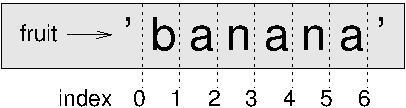
\includegraphics[scale=0.8]{figs/banana.pdf}}
\caption{切片的索引.}
\label{fig.banana}
\end{figure}
如果缺失第一個索引(冒號前), 則切片從字符串頭部開始. 
如果忽略了第二個索引, 切片到末尾結束:

\begin{verbatim}
>>> fruit = 'banana'
>>> fruit[:3]
'ban'
>>> fruit[3:]
'ana'
\end{verbatim}
%
若第一個索引值大於或等於第二個, 則結果為{\bf 空字符串}, 用兩個單引號表示:
\index{quotation mark}

\begin{verbatim}
>>> fruit = 'banana'
>>> fruit[3:3]
''
\end{verbatim}
%
空字符串一般不包括任何字符, 同時長度為0, 除此之外, 
和其他字符串一樣. 

繼續上面的例子, 思考一下{\tt fruit[:]}表示什麼? 試試吧. 
\index{copy!slice}
\index{slice!copy}



\section{字符串不可變}
\index{mutability}
\index{immutability}
\index{string!immutable}

嘗試在賦值等式左側用 {\tt []}操作符修改字符串中的字符. 
例如:
\index{TypeError}
\index{exception!TypeError}

\begin{verbatim}
>>> greeting = 'Hello, world!'
>>> greeting[0] = 'J'
TypeError: 'str' object does not support item assignment
\end{verbatim}
%
這裡的``object''指字符串, ``item''指試圖賦值的字符. 
到目前為止, 你可以認為對像和值一樣, 但是後續
(在第~\ref{equivalence}節), 我們會完善此定義. 
\index{object}
\index{item}
\index{item assignment}
\index{assignment!item}
\index{immutability}

錯誤的原因在於字符串是{\bf 不可變的}, 
也就是說, 你無法改變一個既有的字符串. 
你能做的, 是基於原來字符串做些操作, 創建一個不同的字符串:

\begin{verbatim}
>>> greeting = 'Hello, world!'
>>> new_greeting = 'J' + greeting[1:]
>>> new_greeting
'Jello, world!'
\end{verbatim}
%
上述代碼是用新的首字母和{\tt greeting}的切片進行了拼接, 
而這並不會改變原來的字符串. 
\index{concatenation}


\section{檢索}
\label{find}
下面的函數什麼用途?
\index{find function}
\index{function!find}

\begin{verbatim}
def find(word, letter):
    index = 0
    while index < len(word):
        if word[index] == letter:
            return index
        index = index + 1
    return -1
\end{verbatim}
%
可以認為, {\tt find}是{\tt []}操作符的逆運算. 
此操作不同於根據索引獲取對應字符, 
而是根據字符, 查找其索引. 如果字符沒有檢索到, 
則返回{\tt -1}. 

這是我們第一次見到, 在迴圈內使用{\tt return}語句. 
如果{\tt word[index] == letter}, 函數會跳出迴圈, 並立刻返回結果. 

如果字符串中沒有想要的字符, 程式會一直執行到迴圈結束, 並
返回{\tt -1}.

這種算法--遍歷序列並返回預期結果--叫做{\bf 檢索}. 
\index{traversal}
\index{search pattern}
\index{pattern!search}

做個練習, 為{\tt find}函數加入第三個參數, 一個索引值, 
使其從{\tt word}的此索引處開始檢索.


\section{迴圈和計數}
\label{counter}
\index{counter}
\index{counting and looping}
\index{looping and counting}
\index{looping!with strings}
以下程式會統計字符串中{\tt a}出現的次數:

\begin{verbatim}
word = 'banana'
count = 0
for letter in word:
    if letter == 'a':
        count = count + 1
print(count)
\end{verbatim}
%
此程式描述了另一種算法, 稱之為{\bf 計數器}.
初始化變量{\tt count}為0, 其後每找到一次{\tt a}, 就加1.
迴圈結束後,  {\tt count}便包含了結果-- {\tt a}的全部數量.

\index{encapsulation}
做個練習, 封裝以上代碼為{\tt count}函數, 使其以字符串和字母
為參數, 從而更加通用. 

然後重寫函數, 用上一節的{\tt find}函數的三參數版本, 替換字符串遍歷操作. 


\section{字符串方法}
\label{optional}
字符串提供了諸多有用的方法, 方法類似於函數--輸入參數並返回結果--但是
語法有些不同. 
例如, {\tt upper}方法, 接收字符串, 
並返回一個全部字母大寫後的字符串. 
\index{method}
\index{string!method}

與函數的語法{\tt upper(word)}不同之處在於, 
方法的語法寫作 {\tt word.upper()}.

\begin{verbatim}
>>> word = 'banana'
>>> new_word = word.upper()
>>> new_word
'BANANA'
\end{verbatim}
%
這種點標法, 聲明了方法的名字, {\tt upper}, 
和要使用此方法的字符串的名字, {\tt word}. 
括號為空表明此方法沒有參數. 
\index{parentheses!empty}
\index{dot notation}

令函數運行, 叫做{\bf 調用};
此例中, 我們說調用{\tt word}的{\tt upper}方法. 
\index{invocation}

你會發現, 字符串實際內置了{\tt find}方法, 但和我們寫的函數
驚人相似:

\begin{verbatim}
>>> word = 'banana'
>>> index = word.find('a')
>>> index
1
\end{verbatim}
%
此例中, 我們調用{\tt word}的{\tt find}方法, 將要查找的字母作為入參. 

實際上, {\tt find}方法比我們寫的函數要更通用;
它不僅可以定位字符, 也能定位字符串片段:

\begin{verbatim}
>>> word.find('na')
2
\end{verbatim}
%
默認情況, {\tt find} 從字符串開頭進行查找, 不過也可以給其傳入索引值
作為第二個參數, 
使其從既定位置開始:
\index{optional argument}
\index{argument!optional}

\begin{verbatim}
>>> word.find('na', 3)
4
\end{verbatim}
%
這是一個{\bf 可選參數}的例子;
{\tt find}方法也可以接收第三個索引參數, 以標識結束位置:

\begin{verbatim}
>>> name = 'bob'
>>> name.find('b', 1, 2)
-1
\end{verbatim}
%
{\tt b}沒有出現在字符串索引{\tt 1}和{\tt 2}且不包括{\tt 2}的範圍內, 
所以搜索失敗. 
而這種到達第二個索引位但不包括此索引的規則, 和切片操作一樣. 


\section{操作符 {\tt in}}
\label{inboth}
\index{in operator}
\index{operator!in}
\index{boolean operator}
\index{operator!boolean}

單詞 {\tt in}是一個布爾運算子, 其比較兩個字符串, 
如果前者是後者的一部分, 
則返回{\tt True}:

\begin{verbatim}
>>> 'a' in 'banana'
True
>>> 'seed' in 'banana'
False
\end{verbatim}
%
例如, 下面的函數會輸出同時出現在{\tt word1}和{\tt word2}中的字母:

\begin{verbatim}
def in_both(word1, word2):
    for letter in word1:
        if letter in word2:
            print(letter)
\end{verbatim}
%

變量名選擇得足夠好的話, Python讀起來便如同英語. 
讀一下這個迴圈, ``for (each) letter in (the first) word, if (the) letter 
(appears) in (the second) word, print (the) letter.''

下面是apples和oranges比較的結果:

\begin{verbatim}
>>> in_both('apples', 'oranges')
a
e
s
\end{verbatim}
%

\section{字符串比較}
\index{string!comparison}
\index{comparison!string}

關係運算子同樣適用於字符串. 
比如要判斷兩字符串是否相等:

\begin{verbatim}
if word == 'banana':
    print('All right, bananas.')
\end{verbatim}
%

其他的關係運算子也適用於按照字母順序進行比較:

\begin{verbatim}
if word < 'banana':
    print('Your word, ' + word + ', comes before banana.')
elif word > 'banana':
    print('Your word, ' + word + ', comes after banana.')
else:
    print('All right, bananas.')
\end{verbatim}
%
Python處理大小寫的方式同人類思維不同, 在其看來, 大寫字母都排在小寫字母之前, 
所以:

\begin{verbatim}
 Pineapple 在前,  banana 在後.
\end{verbatim}
%
解決此問題的通常做法是, 在比較前先統一字符串的格式, 比如都轉小寫. 
謹記這一點, 以免遇到Pineapple時, 變得一團糟. 


\section{調試}
\index{debugging}
\index{traversal}

想要用索引來遍歷序列中的值, 難點在於確定遍歷的起點和終點. 
下面是一個比較單詞的函數, 如果一個單詞恰好是另一個單詞的倒序排列, 
則返回{\tt True}, 但這裡有兩處錯誤:

\begin{verbatim}
def is_reverse(word1, word2):
    if len(word1) != len(word2):
        return False
    
    i = 0
    j = len(word2)

    while j > 0:
        if word1[i] != word2[j]:
            return False
        i = i+1
        j = j-1

    return True
\end{verbatim}
%
第一個 {\tt if} 語句會判斷兩個單詞的長度是否一樣. 
如果不同, 立刻返回{\tt False}. 
然而為了執行後續代碼, 我們先假設單詞長度相同. 
這是一個哨兵模式, 在第~\ref{guardian}節已經介紹過. 
\index{guardian pattern}
\index{pattern!guardian}
\index{index}

{\tt i} 和 {\tt j}是索引: {\tt i} 正向遍歷{\tt word1}, 同時{\tt j} 倒序遍歷
{\tt word2}. 如果遇到兩個字母不同, 則即刻返回{\tt False}. 
如果可以通過迴圈檢驗, 則所有字母都匹配, 返回{\tt True}. 

如果用``pots'' 和 ``stop'' 測試函數, 我們期望得到的時{\tt True}, 
但是遇到了索引錯誤:
\index{IndexError}
\index{exception!IndexError}

\begin{verbatim}
>>> is_reverse('pots', 'stop')
...
  File "reverse.py", line 15, in is_reverse
    if word1[i] != word2[j]:
IndexError: string index out of range
\end{verbatim}
%
調試此種異常, 第一步就是在錯誤出現位置前, 先輸出索引的值. 

\begin{verbatim}
    while j > 0:
        print(i, j)        # print here
        
        if word1[i] != word2[j]:
            return False
        i = i+1
        j = j-1
\end{verbatim}
%
再次運行程式, 得到如下信息:

\begin{verbatim}
>>> is_reverse('pots', 'stop')
0 4
...
IndexError: string index out of range
\end{verbatim}
%
首次迴圈,  {\tt j} 的值是4,
超出了\verb"'pots'"的索引範圍. 
最後一個字符的索引應該是3,
所以{\tt j} 的初始值應該是{\tt len(word2)-1}.

如果修復此錯誤, 並再次執行, 輸出如下:

\begin{verbatim}
>>> is_reverse('pots', 'stop')
0 3
1 2
2 1
True
\end{verbatim}
%
這次我們的到了正確結果, 但是迴圈只運行了三次, 有點奇怪. 
為了弄清怎麼回事, 可以繪製堆疊圖來輔助理解. 
第一次疊代, \verb"is_reverse"的狀態框見圖~\ref{fig.state4}.  
\index{state diagram} \index{diagram!state}

\begin{figure}
\centerline
{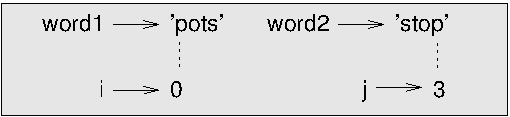
\includegraphics[scale=0.8]{figs/state4.pdf}}
\caption{堆疊圖.}
\label{fig.state4}
\end{figure}

我嘗試在框中對齊變量, 並用虛線標識{\tt i} 和
{\tt j}的值, 用來標識{\tt word1} 和 {\tt word2}中的字符, 
從而幫助理解. 

從此狀態框開始, 在紙上執行程式, 每次疊代時修改{\tt i} 和 {\tt j}值. 
然後找到並修復函數中的第二個錯誤. 
\label{isreverse}


\section{術語表}

\begin{description}

\item[對象(object):] 變量引用的東西, 目前, 可以將
``對象'' 與 ``值'' 同樣看待. 
\index{object}

\item[序列(sequence):] 一些值的有序集合, 每個值都對應一個整數索引. 
\index{sequence}

\item[元素(item):] 序列中的一個值.
\index{item}

\item[索引(index):] 一個整數值, 用來選擇序列中的元素, 
比如選擇字符串中某個字符. Python中的索引都是從0開始. 
\index{index}

\item[切片(slice):] 字符串中一部分, 通過索引範圍確定. 
\index{slice}

\item[空字符串(empty string):] 沒有字符並且長度為0,同時用兩個引號表示的字符串. 
\index{empty string}

\item[不可變(immutable):] 序列中元素不可改變的特性. 
\index{immutability}

\item[遍歷(traverse):] 疊代序列中每個元素, 同時對其執行相似操作的過程. 
\index{traversal}

\item[檢索(search):] 找到預期目標才停止的遍歷模式. 
\index{search pattern}
\index{pattern!search}

\item[計數器(counter):] 用來計數的變量, 一般始於0, 不斷遞增. 
\index{counter}

\item[調用(invocation):] 運行方法的語句.
\index{invocation}

\item[可選參數(optional argument):] 函數或者方法中的不必要參數. 
\index{optional argument}
\index{argument!optional}

\end{description}


\section{習題集}

\begin{exercise}
\index{string method}
\index{method!string}

閱讀文檔\url{http://docs.python.org/3/library/stdtypes.html#string-methods}
中的字符串方法, 
可能你會想試試其中一些方法, 盡量弄明白它們的工作原理. 
{\tt strip} 和 {\tt replace} 特別有用. 

文檔中的某種語法可能難以理解. 
比如\verb"find(sub[, start[, end]])"方法, 方括號標識了可選參數. 
 {\tt sub} 是必需的, 但是{\tt start}是可選的, 
如果包含了 {\tt start}, {\tt end} 便是可選的. 
\index{optional argument}
\index{argument!optional}

\end{exercise}


\begin{exercise}
\index{count method}
\index{method!count}

有個叫{\tt count}的字符串方法, 和第~\ref{counter}節的函數很相似. 
閱讀此方法文檔, 編寫調用此方法的代碼, 實現對\verb"'banana'"中
{\tt a}的個數的統計.
\end{exercise}


\begin{exercise}
\index{step size}
\index{slice operator}
\index{operator!slice}

字符串切片也可以有第三個參數, 叫做``步長'';
也就是, 在連續字符中, 字符間的間距. 
步長為2表示每隔一個字符取一個;
步長為3表示每第三個取一個, 以此類推. 

\begin{verbatim}
>>> fruit = 'banana'
>>> fruit[0:5:2]
'bnn'
\end{verbatim}
步長為-1,則表示倒序讀取, 所以 \verb"[::-1]" 切片, 
便會產生一個倒序的字符串. 
\index{palindrome}

用這個神奇魔法, 將習題~\ref{palindrome}中的 \verb"is_palindrome"
修改為一行代碼的版本吧. 
\end{exercise}


\begin{exercise}

下面的函數都是{\em 試圖}檢驗字符串中是否包含小寫字母, 
但是肯定有函數存在問題. 
仔細分析每個函數並明了其用途
(假設入參都是字符串).

\begin{verbatim}
def any_lowercase1(s):
    for c in s:
        if c.islower():
            return True
        else:
            return False

def any_lowercase2(s):
    for c in s:
        if 'c'.islower():
            return 'True'
        else:
            return 'False'

def any_lowercase3(s):
    for c in s:
        flag = c.islower()
    return flag

def any_lowercase4(s):
    flag = False
    for c in s:
        flag = flag or c.islower()
    return flag

def any_lowercase5(s):
    for c in s:
        if not c.islower():
            return False
    return True
\end{verbatim}

\end{exercise}


\begin{exercise}
\index{letter rotation}
\index{rotation, letter}

\label{exrotate}
凱撒加密(Caesar cypher )是一種通過對每個字母進行特定數值的``移位''操作, 
而實現的簡單加密方案. 
對字母移位, 也就是按照字母順序, 進行移動, 必要時需要回到開頭,  
所以'A'移位3, 得到 'D' ,   'Z' 移位1,得到'A'. 

對一個單詞移位, 就是對每個字母採用相同的移位數量. 
例如``cheer'' 移位7,則為``jolly'',  ``melon''移位-10, 則為 ``cubed''. 
在電影{\em 2001: A Space Odyssey}中, 飛船上的計算機名叫HAL, 
就是IBM移位-1得到的. 

%For example ``sleep''
%rotated by 9 is ``bunny'' and ``latex'' rotated by 7 is ``shale''.

編寫\verb"rotate_word"函數, 接收一個字符串和一個整數, 作為參數, 
對字符串中的字符進行數值移位, 得到新字符串, 並返回. 

你可能需要用內置的{\tt ord}函數, 此函數可以將字符轉為數字碼, 
而{\tt chr}則可以將數字碼轉回字符. 
字母表中的字母會按順序進行編碼, 比如:

\begin{verbatim}
>>> ord('c') - ord('a')
2
\end{verbatim}
因為\verb"'c'"在字母表中是第2個(從0開始)字母. 
但要注意:大寫字母的數字碼和小寫的不同. 

網絡上一些嘲弄有時會採用ROT13編碼, 也就是移位數量為13的凱撒加密. 
如果你不會太介意, 試試解密它們吧. 參閱:
\url{http://thinkpython2.com/code/rotate.py}.

\end{exercise}


\chapter{案例學習: 單詞遊戲}
\label{wordplay}

本章學習第二個案例, 主要研究如何通過搜索特定詞彙, 進行猜謎. 
比如, 查找最長回字文, 以及尋找按照字母表順序排列的單詞. 
同時, 我將介紹一種新的程式開發模式: 抽離紛紛擾擾, 回歸已有方案. 


\section{讀取單詞串列}
\label{wordlist}
本章的練習, 需要準備一個英文單詞串列. 
網上有很多可用的單詞串列, 但是對我們來說, 最理想的莫過於
Grady Ward 收集整理, 作為Moby詞典項目, 貢獻給公共領域的單詞串列
(詳見\url{http://wikipedia.org/wiki/Moby_Project}). 這是
包含 113,809 個填詞遊戲的單詞串列; 也就是說, 這些單詞, 已經被
填詞遊戲和其他單詞遊戲證明了有效. 
在Moby項目中, 這個文件名為 {\tt 113809of.fic};
你可以從\url{http://thinkpython2.com/code/words.txt} 下載一個副本, 
其名字簡稱 {\tt words.txt}. 
\index{Moby Project}
\index{crosswords}

此文件為純文本文件, 你可以用文本編輯器打開, 
但你也可以用Python讀取. 
內置函數{\tt open}, 以文件名為入參, 返回一個 {\bf 文件對象}, 
可以用來讀取文件內容. 
\index{open function}
\index{function!open}
\index{plain text}
\index{text!plain}
\index{object!file}
\index{file object}

\begin{verbatim}
>>> fin = open('words.txt')
\end{verbatim}
%
{\tt fin} 是表示輸入的文件對象的通用名稱. 
文件對象針對讀取提供了多個方法, 包括 {\tt readline}, 此方法會讀取文件的一整行
字符, 並作為字符串返回: \index{readline method}
\index{method!readline}

\begin{verbatim}
>>> fin.readline()
'aa\n'
\end{verbatim}
%
單詞串列中第一個單詞是``aa'', 這是一種岩漿. 
後面的\verb"\n" 是換行符, 用來斷行. 

文件對象會跟蹤目前讀到哪裡了, 從而, 再次運行
{\tt readline}, 會得到後面的單詞:

\begin{verbatim}
>>> fin.readline()
'aah\n'
\end{verbatim}
%
下一個單詞是``aah'',  這是個絕對正確的單詞, 所以別那樣看我. 
另外, 如果換行符令你厭煩, 可以用字符串方法{\tt strip}移除:
\index{strip method}
\index{method!strip}

\begin{verbatim}
>>> line = fin.readline()
>>> word = line.strip()
>>> word
'aahed'
\end{verbatim}
%
你也可以將文件對象置於{\tt for}迴圈中. 
這樣程式便會讀取 {\tt words.txt}, 然後逐行輸出每個單詞:
\index{open function}
\index{function!open}

\begin{verbatim}
fin = open('words.txt')
for line in fin:
    word = line.strip()
    print(word)
\end{verbatim}
%

\section{練習}
下一節有這些習題的答案, 但盡量在看答案之前盡力一試吧. 

\begin{exercise}
編寫程式, 讀取{\tt words.txt}, 僅打印多於20個字符的單詞
(不包括空格). 
\index{whitespace}

\end{exercise}

\begin{exercise}

1939年Ernest Vincent Wright出版了一部 50,000 單詞的小說, 名叫
{\em Gadsby}, 本書不包括字母``e''. 而英文中最常用的便是``e'', 所以
太難得了. 

事實上, 若不使用常用的字符, 一般很難表達出一個觀點. 
不過, 開始雖然進展緩慢, 但是, 通過保持謹慎並訓練幾個小時, 
你也可以慢慢適應. 

好了, 閒言少敘. 

編寫 \verb"has_no_e" 函數, 如果輸入的單詞不包括``e'',  則返回{\tt True}. 

編寫程式, 讀取{\tt words.txt}, 只打印不包含``e''的單詞. 
統計串列中, 不包含``e''的單詞所占比例. 
\index{lipogram}

\end{exercise}


\begin{exercise} 

編寫{\tt avoids}函數, 以單詞和禁用字母字符串為輸入, 當單詞不包含任何禁用字母時, 
返回 {\tt True}. 

編寫程式, 使用戶輸入禁用字母字符串, 
然後輸出不含有這些字母的單詞數量. 
看看你是否可以找出一個包含5個禁用字母的組合, 
使被排除的單詞數最少?

\end{exercise}


\begin{exercise}

編寫函數\verb"uses_only" , 以一個單詞和一串字母為輸入, 
如果單詞的字母都在這串字母中, 則返回{\tt True}.
你是否可以只用{\tt acefhlo}這些字母, 構造出句子?
換成 ``Hoe alfalfa''這些字母呢?

\end{exercise}


\begin{exercise} 

編寫函數\verb"uses_all" , 輸入為一個單詞和一串必需字母, 
如果單詞對這串必需字母, 都至少使用了一次, 則返回{\tt True}. 
看看有多少單詞同時包含{\tt aeiou}? 又有多少同時包含 {\tt aeiouy}呢?

\end{exercise}


\begin{exercise}
編寫函數\verb"is_abecedarian", 如果單詞中的字母是按照字母表順序排列, 
則返回 {\tt True}(字母相同, 視為順序). 看看有多少這種單詞?

\index{abecedarian}

\end{exercise}


\section{檢索}
\label{search}
\index{search pattern}
\index{pattern!search}

上一章節中, 所有的練習, 都有個共通之處;
它們都可以採用第~\ref{find}節的檢索方法來解決. 
舉個簡單例子:

\begin{verbatim}
def has_no_e(word):
    for letter in word:
        if letter == 'e':
            return False
    return True
\end{verbatim}
%
{\tt for}迴圈會遍歷 {\tt word}中所有字母. 
如果遇到 ``e'', 則即刻返回{\tt False};
否則繼續下一個字母. 
如果迴圈正常結束, 也就是說沒有遇到``e'',  則返回{\tt True}.
\index{traversal}

\index{in operator}
\index{operator!in}
你也可以使用{\tt in}運算子來精簡程式, 
我先介紹上述版本, 主要是闡述清楚檢索算法的內在邏輯. 

\index{generalization}
{\tt avoids} 函數相比 \verb"has_no_e" 版本, 功能更加通用, 
但結構相同:

\begin{verbatim}
def avoids(word, forbidden):
    for letter in word:
        if letter in forbidden:
            return False
    return True
\end{verbatim}
%
在此函數中, 一旦遇到禁止字母, 即刻返回{\tt False}, 
如果迴圈終了, 則返回{\tt True}. 

\verb"uses_only" 與之極為相似, 無非條件相反:

\begin{verbatim}
def uses_only(word, available):
    for letter in word: 
        if letter not in available:
            return False
    return True
\end{verbatim}
%
這裡不再是禁用字母串列了, 而是可用字母串列. 
如果 {\tt word}中出現了不在可用串列中的字母, 返回{\tt False}.

\verb"uses_all"和上述函數也較為相似, 不同之處在於, 
我們交換了單詞和字母序列的角色:

\begin{verbatim}
def uses_all(word, required):
    for letter in required: 
        if letter not in word:
            return False
    return True
\end{verbatim}
%
不再是遍歷 {\tt word}中的字母, 
而是遍歷必需字母串列. 
如果字母串列中有字母未出現在單詞中, 返回{\tt False}.
\index{traversal}

如若你已像電腦科學家一樣去思考, 你便會注意到 \verb"uses_all" 
是以前一個已解決的問題的另一種表達, 你便會這麼寫:

\begin{verbatim}
def uses_all(word, required):
    return uses_only(required, word)
\end{verbatim}
%
此案例便是一個{\bf 抽離紛擾, 回歸已知}的程式開發模式的實踐, 
這種模式是將遇到的問題, 映射為已解決的問題, 
從而用已有的解決方案來解決當前問題.   
\index{reduction to a previously solved problem} 
\index{development plan!reduction}


\section{索引迴圈}
\index{looping!with indices}
\index{index!looping with}
前一章節中, 我用{\tt for}迴圈編寫了大量函數, 這是因為我
只關注字符串中的字符; 所以無需關注索引. 

但\verb"is_abecedarian"函數中, 我們不得不比較相鄰的字母, 
用{\tt for}迴圈便不太方便:

\begin{verbatim}
def is_abecedarian(word):
    previous = word[0]
    for c in word:
        if c < previous:
            return False
        previous = c
    return True
\end{verbatim}

用遞歸來實現:

\begin{verbatim}
def is_abecedarian(word):
    if len(word) <= 1:
        return True
    if word[0] > word[1]:
        return False
    return is_abecedarian(word[1:])
\end{verbatim}

還可以使用 {\tt while} 迴圈:

\begin{verbatim}
def is_abecedarian(word):
    i = 0
    while i < len(word)-1:
        if word[i+1] < word[i]:
            return False
        i = i+1
    return True
\end{verbatim}
%
此迴圈始於 {\tt i=0}, 終於{\tt i=len(word)-1}. 
每次迴圈都會比較第$i$個字符(可以看作當前字符)
和第$i+1$個字符(可以看作後一個字符). 

如果後一個字符小於(在字母表順序中先於)當前字符, 
我們會發現這和要求不符, 便返回{\tt False}.

如果直到迴圈末尾, 仍然無異常, 則單詞合格. 
為確信迴圈正常結束, 可以試試\verb"'flossy'". 
單詞長度為6, 所以{\tt i} 為 4時, 便是最後一次迴圈, 
因為這是倒數第二個字符的索引. 最後一次迴圈中, 
比較了倒數第二個和倒數第一個字符, 這恰恰符合預期. 
\index{palindrome}

下面是\verb"is_palindrome" 函數(參看習題~\ref{palindrome})的另一個版本, 
其使用了兩個索引; 一個從開頭到結尾, 順序前進;
另一個從結尾到開頭, 倒序進行.

\begin{verbatim}
def is_palindrome(word):
    i = 0
    j = len(word)-1

    while i<j:
        if word[i] != word[j]:
            return False
        i = i+1
        j = j-1

    return True
\end{verbatim}

或者, 我們映射到以前解決過的難題, 進行重寫:
\index{reduction to a previously solved problem}
\index{development plan!reduction}

\begin{verbatim}
def is_palindrome(word):
    return is_reverse(word, word)
\end{verbatim}
%
此處使用了第~\ref{isreverse}節的\verb"is_reverse"函數.


\section{調試}
\index{debugging}
\index{testing!is hard}
\index{program testing}

程式測試很難. 本章的函數相對容易測試, 因為你可以用手算來檢驗結果. 
即便如此, 要選擇一批單詞, 測試所有可能錯誤, 那便難上加難了. 

以\verb"has_no_e"為例, 需要檢驗兩種情景: 一種是含有`e'的單詞, 返回{\tt False}, 
另一種是不含有`e'的單詞, 返回{\tt True}. 
對此, 你應該很容易針對每種情景, 都想出一個單詞. 

對於每種情景, 存在一些不太明顯的子用例. 
對於包含 ``e''的單詞, 你需要檢驗 ``e''在開頭的, 在結尾的, 甚至中間某些位置的單詞. 
你要檢驗長單詞, 短單詞, 甚至非常短的單詞, 比如空字符串. 
空字符串是{\bf 特例}的一種, 也就是那種容易被忽視, 卻往往是錯誤頻發之處的用例. 
\index{special case}

除了自己構建測試用例, 你也可以用類似{\tt words.txt}的單詞串列檢驗程式. 
通過掃描輸出, 你可能會發現錯誤, 但要注意: 
你可能發現了某種錯誤(包括了不應包含的單詞), 而忽略了其他錯誤
(沒有包括應該包含的單詞). 

通常, 程式測試可以幫助你發現錯誤, 但要製作出好的測試用例, 
往往很難, 即使通過了這些測試, 你也不能百分百地確認你的程式正確. 
一位傳奇的電腦科學家說過:
\index{testing!and absence of bugs}

\begin{quote}

程式測試只能表明錯誤的存在, 卻永遠無法保證其不存在!

--- Edsger W. Dijkstra
\end{quote}
\index{Dijkstra, Edsger}


\section{術語表}

\begin{description}

\item[文件對象(file object):] 用來標識被打開的文件的一個值.
\index{file object}
\index{object!file}

\item[抽離紛繞, 回歸已知(reduction to a previously solved problem):] 一種將當前問題簡化為已解決問題, 進而解決問題的方式.
\index{reduction to a previously solved problem}
\index{development plan!reduction}

\item[特例(special case):] 非典型或者不明顯的測試用例
(往往容易犯錯的地方).
\index{special case}

\end{description}


\section{習題集}

\begin{exercise}
\index{Car Talk}
\index{Puzzler}
\index{double letters}

這個問題源於廣播節目 {\em Car Talk} 中的一個謎題
(\url{http://www.cartalk.com/content/puzzlers}):

\begin{quote}
給我一個存在三個連續雙字母的單詞. 
我會給你一些看似符合, 其實不符的單詞. 
例如, 單詞committee,  c-o-m-m-i-t-t-e-e. 
如果沒有`i' 在中間, 就很完美. 
又或者Mississippi: M-i-s-s-i-s-s-i-p-p-i.
如果將其中的 i 都移除, 便符合了. 
但是有一個詞恰好含有三個連續雙字母, 而且據我所知, 
這可能是僅有的一個這樣的單詞. 
當然, 實際上有可能有500多個這樣的單詞, 但我只能想到一個. 
是哪個單詞呢?
\end{quote}

編寫程式來尋找一下吧. 
答案: \url{http://thinkpython2.com/code/cartalk1.py}.

\end{exercise}


\begin{exercise}
這也是一個 {\em Car Talk}的謎題(\url{http://www.cartalk.com/content/puzzlers}):
\index{Car Talk}
\index{Puzzler}
\index{odometer}
\index{palindrome}

\begin{quote}

``某天我在高速上開車, 碰巧注意到里程表. 
同多數里程表一樣, 它有6個數字, 只能表示整裡數. 
所以, 如果我的車跑了300,000英里, 那顯示的就是
3-0-0-0-0-0.

``現在, 我看到的很有意思. 最後4個數字是回文;也就是說, 從前往後讀
和從後往前讀都一樣. 比如5-4-4-5 便是個回文, 
所以我的里程表可能顯示的是3-1-5-4-4-5.

``一英里後, 最後的5個數字也是回文. 
例如顯示為3-6-5-4-5-6. 然後又跑了1英里, 6個數字中間的4位是回文了. 
準備好玩這個了嗎? 那又跑了1英里, 所有6個數字也是回文了!

``問題來了, 我開始在里程表上看到的數字是什麼?''
\end{quote}

編寫個Python程式, 檢驗所有的6位數字, 然後輸出滿足上述要求的任意數字. 
答案: \url{http://thinkpython2.com/code/cartalk2.py}.

\end{exercise}


\begin{exercise}
再來一個{\em Car Talk}上的謎題, 你可以用檢索法來
解決(\url{http://www.cartalk.com/content/puzzlers}):
\index{Car Talk}
\index{Puzzler}
\index{palindrome}

\begin{quote}
``最近我去看望母親, 我們發現我的年齡倒過來, 正好是母親的年齡. 
比如, 若她是73, 我是37. 我們想知道在過去這些年, 有多少次這種情況發生, 
但後來我們岔開了話題, 沒有得到答案. 

``回到家後, 我發現到目前為止, 我們的年齡已經互逆了6次. 
同時, 我也意識到, 如果我們幸運的話, 稍後幾年, 我們又會年齡互逆一次, 
如果我們特別幸運, 就還會有一次機會. 換句話說, 這樣的情況, 可能我們一共會
遇到8次. 所以, 請問, 我現在多少歲了?''

\end{quote}

編寫Python程式, 尋找這個謎題的答案. 
提示: 你可能會用到字符串的 {\tt zfill} 方法. 

答案: \url{http://thinkpython2.com/code/cartalk3.py}.

\end{exercise}



\chapter{串列}

本章講述Python最有用的內置類型, 串列. 
同時你會深入了解對象, 學習一個對象對應多個名稱時會產生的現象. 


\section{串列即序列}
\label{sequence}

同字符串一樣, {\bf 串列} 也是值的序列. 
字符串中, 值是字符;在串列中, 值可以是任何類型. 
串列中的值, 叫做{\bf 元素}, 有時也叫{\bf 串列項}.
\index{list}
\index{type!list}
\index{element}
\index{sequence}
\index{item}

創建串列的方式很多; 最簡單的莫過於將元素用方括號包起來(\verb"[" and \verb"]"):

\begin{verbatim}
[10, 20, 30, 40]
['crunchy frog', 'ram bladder', 'lark vomit']
\end{verbatim}
%
第一個例子是由四個整數構成的串列, 
第二個示例串列則由三個字符串構成. 
串列中的元素類型可以不同. 
下面的串列, 便同時包括了字符串, 浮點數, 整數以及另一個串列:

\begin{verbatim}
['spam', 2.0, 5, [10, 20]]
\end{verbatim}
%
串列中包含串列, 叫做{\bf 嵌套串列}.
\index{nested list}
\index{list!nested}

不包含任何元素的串列, 叫做空串列;
你可以用\verb"[]"創建空串列.
\index{empty list}
\index{list!empty}

如你所想, 串列也可以賦給變量:

\begin{verbatim}
>>> cheeses = ['Cheddar', 'Edam', 'Gouda']
>>> numbers = [42, 123]
>>> empty = []
>>> print(cheeses, numbers, empty)
['Cheddar', 'Edam', 'Gouda'] [42, 123] []
\end{verbatim}
%
\index{assignment}


\section{串列可變}
\label{mutable}
\index{list!element}
\index{access}
\index{index}
\index{bracket operator}
\index{operator!bracket}

從串列中獲取元素的語法和從字符串中獲取字符的語法一樣--方括號操作符. 
括號中的表達式確定了索引值. 
要注意, 索引從0開始:

\begin{verbatim}
>>> cheeses[0]
'Cheddar'
\end{verbatim}
%
和字符串不同, 串列是可變的, 當括號操作符出現在賦值語句左側, 
就會將對應的串列元素重新賦值. 
\index{mutability}

\begin{verbatim}
>>> numbers = [42, 123]
>>> numbers[1] = 5
>>> numbers
[42, 5]
\end{verbatim}
%
{\tt numbers}中的第一個元素, 原來是123,現在變成了5.
\index{index!starting at zero}
\index{zero, index starting at}


圖~\ref{fig.liststate} 是 {\tt cheeses}, {\tt numbers} 和{\tt empty} 的狀態圖.
\index{state diagram}
\index{diagram!state}

\begin{figure}
\centerline
{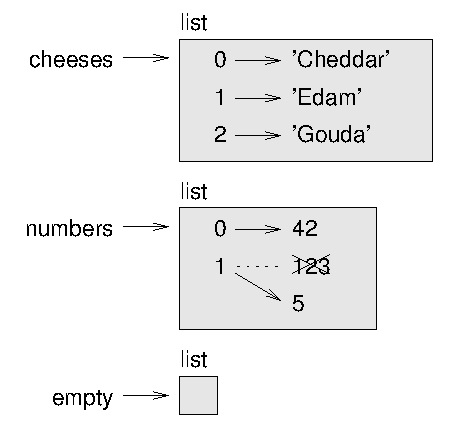
\includegraphics[scale=0.8]{figs/liststate.pdf}}
\caption{狀態圖.}
\label{fig.liststate}
\end{figure}

串列用單詞``list''在外, 元素在內的箱體圖表示. 
{\tt cheeses} 指向了一個包括三個元素的串列, 其索引分別為0,1和2. 
{\tt numbers} 包括兩個元素; 圖中也展現了第二個元素從123 被賦值為5的過程. 
{\tt empty} 指向了一個空串列. 
\index{item assignment}
\index{assignment!item}
\index{reassignment}

串列索引和字符串索引的作用是一樣的:

\begin{itemize}

\item 索引可以是任意整型表達式.

\item 如果試圖通過索引讀寫不存在的元素, 會得到{\tt IndexError}.
\index{exception!IndexError}
\index{IndexError}

\item 如果索引為負值, 則從串列末尾倒序計數. 

\end{itemize}
\index{list!index}

\index{list!membership}
\index{membership!list}
\index{in operator}
\index{operator!in}

運算子{\tt in}也可作用於串列. 

\begin{verbatim}
>>> cheeses = ['Cheddar', 'Edam', 'Gouda']
>>> 'Edam' in cheeses
True
>>> 'Brie' in cheeses
False
\end{verbatim}


\section{遍歷串列}
\index{list!traversal}
\index{traversal!list}
\index{for loop}
\index{loop!for}
\index{statement!for}

遍歷串列中元素的最常用方法便是{\tt for}迴圈. 語法和字符串遍歷相同:

\begin{verbatim}
for cheese in cheeses:
    print(cheese)
\end{verbatim}
%
這種方法對於僅讀取串列中元素很方便, 但是如果你想寫入或者更新元素, 
那便需要索引了. 
通常把內置函數{\tt range} 和 {\tt len}結合使用:
\index{looping!with indices}
\index{index!looping with}

\begin{verbatim}
for i in range(len(numbers)):
    numbers[i] = numbers[i] * 2
\end{verbatim}
%

此迴圈會遍歷串列並更新每個元素. 
{\tt len}方法會返回串列中元素數量. {\tt range} 則返回從0到 $n-1$的索引值串列, 
其中 $n$ 是串列的長度. 
每次迴圈, {\tt i}都會獲得下一個元素的索引. 迴圈體中的賦值語句
則會通過{\tt i}獲取元素的舊值, 並賦予新值. 
\index{item update}
\index{update!item}

用{\tt for}迴圈遍歷空串列, 永遠不會執行迴圈體:

\begin{verbatim}
for x in []:
    print('This never happens.')
\end{verbatim}
%
雖然串列可以包含其他串列, 但是嵌入的串列仍表示一個元素. 
下面串列的長度為{\tt 4}:
\index{nested list}
\index{list!nested}

\begin{verbatim}
['spam', 1, ['Brie', 'Roquefort', 'Pol le Veq'], [1, 2, 3]]
\end{verbatim}



\section{串列操作}
\index{list!operation}

運算子 {\tt +} 可以用來拼接串列:
\index{concatenation!list}
\index{list!concatenation}

\begin{verbatim}
>>> a = [1, 2, 3]
>>> b = [4, 5, 6]
>>> c = a + b
>>> c
[1, 2, 3, 4, 5, 6]
\end{verbatim}
%

運算子 {\tt *} 會將串列複製給定的次數:
\index{repetition!list}
\index{list!repetition}

\begin{verbatim}
>>> [0] * 4
[0, 0, 0, 0]
>>> [1, 2, 3] * 3
[1, 2, 3, 1, 2, 3, 1, 2, 3]
\end{verbatim}
%
第一個示例複製了{\tt [0]}四次. 
第二個, 則複製了{\tt [1, 2, 3]}三次. 


\section{串列切片}
\index{slice operator}
\index{operator!slice}
\index{index!slice}
\index{list!slice}
\index{slice!list}

切片運算子同樣適用於串列:

\begin{verbatim}
>>> t = ['a', 'b', 'c', 'd', 'e', 'f']
>>> t[1:3]
['b', 'c']
>>> t[:4]
['a', 'b', 'c', 'd']
>>> t[3:]
['d', 'e', 'f']
\end{verbatim}
%
如果省略第一位索引, 則從頭開始, 進行切片. 
如果省略第二位索引, 則切片止於末尾. 
如果兩位都省略, 則切片便等同於複製整個串列. 
\index{list!copy}
\index{slice!copy}
\index{copy!slice}

\begin{verbatim}
>>> t[:]
['a', 'b', 'c', 'd', 'e', 'f']
\end{verbatim}
%
因為串列可變, 所以最好在執行修改串列的操作前, 複製一份, 以防萬一. 
\index{mutability}

如果切片運算子在賦值號左側, 便可以同時更新多個元素:
\index{slice!update}
\index{update!slice}

\begin{verbatim}
>>> t = ['a', 'b', 'c', 'd', 'e', 'f']
>>> t[1:3] = ['x', 'y']
>>> t
['a', 'x', 'y', 'd', 'e', 'f']
\end{verbatim}
%

% 你也可以通過將待更新元素放入空的位置, 從而向串列添加元素
% :

% % \begin{verbatim}
% >>> t = ['a', 'd', 'e', 'f']
% >>> t[1:1] = ['b', 'c']
% >>> print t
% ['a', 'b', 'c', 'd', 'e', 'f']
% \end{verbatim}
% \afterverb
%
% 也可以通過賦值空串列, 從而移除元素. 
% :

% % \begin{verbatim}
% >>> t = ['a', 'b', 'c', 'd', 'e', 'f']
% >>> t[1:3] = []
% >>> print t
% ['a', 'd', 'e', 'f']
% \end{verbatim}
% \afterverb
%
% 但這些操作都可以用更加清晰明瞭的串列方法替換
% .


\section{串列方法}
\index{list!method}
\index{method, list}

Python 提供了大量操作串列的方法. 例如, 
{\tt append} 可以在串列末尾添加新元素:
\index{append method}
\index{method!append}

\begin{verbatim}
>>> t = ['a', 'b', 'c']
>>> t.append('d')
>>> t
['a', 'b', 'c', 'd']
\end{verbatim}
%
{\tt extend}會以串列為參數, 並將其中所有元素添加到執行串列中:
\index{extend method}
\index{method!extend}

\begin{verbatim}
>>> t1 = ['a', 'b', 'c']
>>> t2 = ['d', 'e']
>>> t1.extend(t2)
>>> t1
['a', 'b', 'c', 'd', 'e']
\end{verbatim}
%
這個例子中, {\tt t2} 沒有被修改. 

{\tt sort} 會將串列元素, 從低到高排序:
\index{sort method}
\index{method!sort}

\begin{verbatim}
>>> t = ['d', 'c', 'e', 'b', 'a']
>>> t.sort()
>>> t
['a', 'b', 'c', 'd', 'e']
\end{verbatim}
%
多數串列方法都沒有返回值; 這些方法修改串列然後返回{\tt None}. 
如果你意外寫了{\tt t = t.sort()}, 結果會令你失望. 
\index{void method}
\index{method!void}
\index{None special value}
\index{special value!None}


\section{Map, filter和reduce}
\label{filter}

若想對串列中所有數字求和, 可以用如下迴圈實現:

% see add.py

\begin{verbatim}
def add_all(t):
    total = 0
    for x in t:
        total += x
    return total
\end{verbatim}
%
{\tt total}初始為0.
每迴圈一次{\tt x} 會從串列中獲取一個元素. {\tt +=} 操作符, 是一種更新運算的便捷寫法. 
也是一種 {\bf 增量賦值語句}. 
\index{update operator}
\index{operator!update}
\index{assignment!augmented}
\index{augmented assignment}

\begin{verbatim}
    total += x
\end{verbatim}
%
等同於

\begin{verbatim}
    total = total + x
\end{verbatim}
%
隨著迴圈運行, {\tt total} 會累積元素求和;
這樣的變量有時也稱為{\bf 累加器}. 
\index{accumulator!sum}
對串列元素求和, 使用比較普遍, 所以Python提供了內置函數{\tt sum}:

\begin{verbatim}
>>> t = [1, 2, 3]
>>> sum(t)
6
\end{verbatim}
%
像這樣將一系列元素合為一個值的操作, 一般稱為{\bf reduce}.
\index{reduce pattern}
\index{pattern!reduce}
\index{traversal}

有時, 你會遍歷串列, 創建新串列. 例如, 下述函數會接收字符串串列, 
並返回一個將所有字符串都轉為首字母大寫的字符串串列:

\begin{verbatim}
def capitalize_all(t):
    res = []
    for s in t:
        res.append(s.capitalize())
    return res
\end{verbatim}
%
{\tt res} 開始是一個空串列; 每次迴圈, 都會向其中添加下一個元素. 
所以{\tt res}也可認為是另一種累加器. 
\index{accumulator!list}

類似\verb"capitalize_all"這樣的操作, 一般叫做{\bf map}, 
因為此操作會將函數(此處為{\tt capitalize})``應用''到序列中每個元素上. 
\index{map pattern}
\index{pattern!map}
\index{filter pattern}
\index{pattern!filter}

另一種常用操作是, 從串列中篩選部分元素, 返回子串列. 例如, 
下面函數會接收一個字符串串列, 返回僅包含大寫字母的字符串串列:

\begin{verbatim}
def only_upper(t):
    res = []
    for s in t:
        if s.isupper():
            res.append(s)
    return res
\end{verbatim}
%
{\tt isupper}是字符串方法, 如果字符串中字母全部為大寫, 則返回{\tt True}. 

如\verb"only_upper" 一樣的操作, 叫做 {\bf filter}, 因為此操作會篩選出某些元素, 
過濾掉其他元素. 

大部分的串列操作都可以由map, filter 以及reduce 組合構成. 


\section{移除元素}
\index{element deletion}
\index{deletion, element of list}

從串列中移除元素有多種方法. 
如果你知道所要移除元素的索引, 可以用
{\tt pop}方法:
\index{pop method}
\index{method!pop}

\begin{verbatim}
>>> t = ['a', 'b', 'c']
>>> x = t.pop(1)
>>> t
['a', 'c']
>>> x
'b'
\end{verbatim}
%
{\tt pop} 會改變串列, 並返回被移除的元素. 
如果未提供索引, 則會刪除並返回最後一個元素. 

如果你不使用移除的元素, 則可以用{\tt del}元算符:
\index{del operator}
\index{operator!del}

\begin{verbatim}
>>> t = ['a', 'b', 'c']
>>> del t[1]
>>> t
['a', 'c']
\end{verbatim}
%
如果你知道要刪除元素的值(但不知道索引位置), 你可以用{\tt remove}方法:
\index{remove method}
\index{method!remove}

\begin{verbatim}
>>> t = ['a', 'b', 'c']
>>> t.remove('b')
>>> t
['a', 'c']
\end{verbatim}
%
{\tt remove} 方法的返回值是{\tt None}.
\index{None special value}
\index{special value!None}

如果要移除多個元素, 可以用 {\tt del}配合切片索引實現:

\begin{verbatim}
>>> t = ['a', 'b', 'c', 'd', 'e', 'f']
>>> del t[1:5]
>>> t
['a', 'f']
\end{verbatim}
%
通常, 切片含頭不含尾, 即到第二個索引值(不包括)為止. 



\section{串列和字符串}
\index{list}
\index{string}
\index{sequence}

字符串是一系列的字符, 串列是一系列的值, 但是字符串列和字符串並不可等同視之. 
採用 {\tt list}方法, 可以將字符串轉換為字符串列:
\index{list!function}
\index{function!list}

\begin{verbatim}
>>> s = 'spam'
>>> t = list(s)
>>> t
['s', 'p', 'a', 'm']
\end{verbatim}
%
因{\tt list}是一個內置函數的名字, 所以盡量避免將其作為變量名. 
我通常也不建議使用{\tt l} , 因為和{\tt 1}太像了. 這便是我用
{\tt t}作為變量名的緣由. 

{\tt list}函數可以將字符串拆解為單獨的字母. 
如果你想將字符串分拆為一個個單詞, 則可以使用{\tt split}方法:
\index{split method}
\index{method!split}

\begin{verbatim}
>>> s = 'pining for the fjords'
>>> t = s.split()
>>> t
['pining', 'for', 'the', 'fjords']
\end{verbatim}
%
此處的可選參數是{\bf 分隔符}, 也就是定義單詞邊界的字符. 
下面的示例使用連字符作為分隔符:
\index{optional argument}
\index{argument!optional}
\index{delimiter}

\begin{verbatim}
>>> s = 'spam-spam-spam'
>>> delimiter = '-'
>>> t = s.split(delimiter)
>>> t
['spam', 'spam', 'spam']
\end{verbatim}
%
{\tt join}和 {\tt split}的作用正好相反. 
它會接收字符串串列, 然後拼接所有元素. 
{\tt join}是一個字符串方法, 所以你需要
在分隔符上調用此方法, 然後將串列作為參數傳入:
\index{join method}
\index{method!join}
\index{concatenation}

\begin{verbatim}
>>> t = ['pining', 'for', 'the', 'fjords']
>>> delimiter = ' '
>>> s = delimiter.join(t)
>>> s
'pining for the fjords'
\end{verbatim}
%
此例中, 分隔符是一個空格, 
{\tt join}會在每個單詞之間放置一個空格. 
若想不用空格拼接, 則可以用空字符串\verb"''"作為分隔符. 
\index{empty string}
\index{string!empty}


\section{對象和值}
\label{equivalence}
\index{object}
\index{value}

如果運行下面的賦值語句:

\begin{verbatim}
a = 'banana'
b = 'banana'
\end{verbatim}
%
我們知道{\tt a} 和 {\tt b}都指向了字符串, 但我們不知道, 他們是否指向
了{\em 相同的} 字符串. 
所以, 便有了兩種可能狀態, 如圖~\ref{fig.list1}.
\index{aliasing}

\begin{figure}
\centerline
{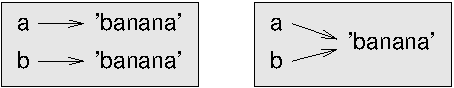
\includegraphics[scale=0.8]{figs/list1.pdf}}
\caption{狀態圖.}
\label{fig.list1}
\end{figure}

第一種情況, {\tt a} 和 {\tt b}指向了兩個不同對象, 這兩個對象
有相同的值. 第二種情況, 它們指向了同一個對象. 
\index{is operator}
\index{operator!is}

若想判斷兩個變量是否指向了同一個對象, 可以用{\tt is}運算子.

\begin{verbatim}
>>> a = 'banana'
>>> b = 'banana'
>>> a is b
True
\end{verbatim}
%
此例中, Python僅創建了一個字符串對象, 然後{\tt a} 
和 {\tt b} 都指向了此對象. 
但是當你創建兩個串列時, 你得到的就是兩個對象:

\begin{verbatim}
>>> a = [1, 2, 3]
>>> b = [1, 2, 3]
>>> a is b
False
\end{verbatim}
%

此時, 狀態圖便是圖~\ref{fig.list2}的樣子.
\index{state diagram}
\index{diagram!state}

\begin{figure}
\centerline
{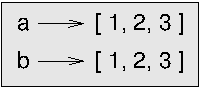
\includegraphics[scale=0.8]{figs/list2.pdf}}
\caption{狀態圖.}
\label{fig.list2}
\end{figure}

這種情況下, 可以說這兩個串列是{\bf 相等的},
因為它們有相同的元素, 
但它們不是{\bf 相同的}, 因為不是同一個對象. 
兩個對象如果相同, 那麼它們必然相等, 
但是它們如果相等, 卻未必相同. 
\index{equivalence}
\index{identity}

到目前為止, 我們一直混用``對象''和 ``值'', 但更準確地說, 
一個對象有一個值. 若創建{\tt [1, 2, 3]}, 你會得到一個串列對象, 
而這個對象的值是個整數序列. 
如果另外一個串列也有相同的元素, 我們便說它們擁有相同的值, 
但它們不是同一個對象. 
\index{object}
\index{value}


\section{別稱}
\index{aliasing}
\index{reference!aliasing}

如果 {\tt a} 指向一個對象, 同時令{\tt b = a},
那麼, 兩個變量都指向了同一個對象:

\begin{verbatim}
>>> a = [1, 2, 3]
>>> b = a
>>> b is a
True
\end{verbatim}
%
此時狀態圖如圖~\ref{fig.list3}所示.
\index{state diagram}
\index{diagram!state}

\begin{figure}
\centerline
{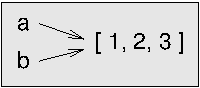
\includegraphics[scale=0.8]{figs/list3.pdf}}
\caption{狀態圖.}
\label{fig.list3}
\end{figure}

變量和對像的這種關聯, 叫做{\bf 引用}.
上例中, 兩個引用指向了同一個對象. 
\index{reference}

有多個引用的對象, 也便有了多個名稱, 
如此, 我們可以說, 對象是有{\bf 別稱的}.
\index{mutability}

如果一個有別稱的對象是可變的, 那麼一個別稱所做的修改會影響另一個:

\begin{verbatim}
>>> b[0] = 42
>>> a
[42, 2, 3]
\end{verbatim}
%

雖然此特性很有用, 但也很容易出錯. 
通常, 對於可變對象, 避免使用別稱, 會安全很多. 
\index{immutability}

而對於像字符串這樣的不可變對象, 別稱使用往往不是問題. 
如下所示:

\begin{verbatim}
a = 'banana'
b = 'banana'
\end{verbatim}
%
所以{\tt a} 和 {\tt b} 是否指向同一個對象, 已無關緊要. 


\section{串列參數}
\label{list.arguments}
\index{list!as argument}
\index{argument}
\index{argument!list}
\index{reference}
\index{parameter}

當給函數傳遞串列時, 函數收到的是對該串列的引用. 
如果函數修改了串列, 那麼調用一方也會看到相應變化. 
例如, \verb"delete_head" 函數刪除了串列中第一個元素:

\begin{verbatim}
def delete_head(t):
    del t[0]
\end{verbatim}
%

下面是一個應用:

\begin{verbatim}
>>> letters = ['a', 'b', 'c']
>>> delete_head(letters)
>>> letters
['b', 'c']
\end{verbatim}
%
形參{\tt t}和變量{\tt letters}是同一個變量的別稱. 
堆疊圖如圖~\ref{fig.stack5}所示.
\index{stack diagram}
\index{diagram!stack}

\begin{figure}
\centerline
{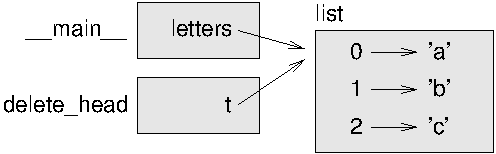
\includegraphics[scale=0.8]{figs/stack5.pdf}}
\caption{堆疊圖.}
\label{fig.stack5}
\end{figure}

因兩個框共用一個串列, 所以我把串列畫在了它們中間. 

區分修改串列操作和新建串列操作, 是非常重要的. 
例如,  {\tt append}方法是修改串列, 而{\tt +}運算子則會新建串列.
\index{append method}
\index{method!append}
\index{list!concatenation}
\index{concatenation!list}

下面是{\tt append}的一個使用示例:
%
\begin{verbatim}
>>> t1 = [1, 2]
>>> t2 = t1.append(3)
>>> t1
[1, 2, 3]
>>> t2
None
\end{verbatim}
%
{\tt append} 的返回值是 {\tt None}.

下面是使用 {\tt +}運算子的示例:
%
\begin{verbatim}
>>> t3 = t1 + [4]
>>> t1
[1, 2, 3]
>>> t3
[1, 2, 3, 4]
\end{verbatim}
%
操作結果是個新串列, 原串列也沒有變化.

在為修改串列而編寫函數時, 此差異尤要重視. 
例如, 下面函數{\em 沒有}刪除串列的第一個元素:
%
\begin{verbatim}
def bad_delete_head(t):
    t = t[1:]              # WRONG!
\end{verbatim}
%
此切片運算子會新建串列, 同時賦值號令 {\tt t}指向此新串列, 
但是這個操作並不會影響調用者.
\index{slice operator}
\index{operator!slice}
%
\begin{verbatim}
>>> t4 = [1, 2, 3]
>>> bad_delete_head(t4)
>>> t4
[1, 2, 3]
\end{verbatim}
%

\verb"bad_delete_head"函數開始運行時, {\tt t} 和 {\tt t4} 指向了同一個
串列. 函數結束時, {\tt t}指向了新的串列, 
但是{\tt t4} 仍然指向了原來的,未被修改的串列.

一種替代方案是, 編寫一個創建並返回新串列的函數. 比如, 
{\tt tail}函數會返回串列中除首元素的所有元素串列:

\begin{verbatim}
def tail(t):
    return t[1:]
\end{verbatim}
%
此函數依然會保持原串列不變. 下面是用法:

\begin{verbatim}
>>> letters = ['a', 'b', 'c']
>>> rest = tail(letters)
>>> rest
['b', 'c']
\end{verbatim}



\section{調試}
\index{debugging}

若使用串列(和其他可變對象)時不夠小心謹慎, 很容易導致長達數小時的調試跟蹤. 
這裡有一些常見陷阱以及如何避免:

\begin{enumerate}

\item 多數的串列方法都是傳入參數, 返回 {\tt None}. 
這和字符串方法恰恰相反, 字符串方法一般返回新字符串, 
同時保持原始值不變. 

如果你慣於編寫下面這樣的代碼:

\begin{verbatim}
word = word.strip()
\end{verbatim}

那麼你可能會寫出下面這樣的代碼:

\begin{verbatim}
t = t.sort()           # WRONG!
\end{verbatim}
\index{sort method}
\index{method!sort}

因為 {\tt sort}返回的是{\tt None}, 所以後續對{\tt t}的操作多會失敗.

在使用串列方法前, 你應該認真閱讀文檔, 並在交互模式下測試一下. 

\item 確定原則, 堅定執行.

串列使用中面臨的部分問題在於, 有多條道路通羅馬. 
比如, 從串列中移除元素, 你可以用 {\tt pop}, {\tt remove}, {\tt del},
甚至用切片重新賦值. 

若想給串列添加元素, 可以用{\tt append}方法, 或者{\tt +}運算子. 
假設{\tt t}是串列, {\tt x}是串列元素, 下面的操作都正確: 

\begin{verbatim}
t.append(x)
t = t + [x]
t += [x]
\end{verbatim}

而下面的代碼是錯誤的:

\begin{verbatim}
t.append([x])          # WRONG!
t = t.append(x)        # WRONG!
t + [x]                # WRONG!
t = t + x              # WRONG!
\end{verbatim}

在交互模式下測試每個示例, 確保理解其作用. 
你會注意到, 只有最後一個會報運行時異常;
其他三個語句合法, 但並不會得到想要的效果. 


\item 複製串列, 避免別稱.
\index{aliasing!copying to avoid}
\index{copy!to avoid aliasing}

你若想使用{\tt sort} 方法修改參數, 同時又想保留原串列, 那你可以複製一份. 

\begin{verbatim}
>>> t = [3, 1, 2]
>>> t2 = t[:]
>>> t2.sort()
>>> t
[3, 1, 2]
>>> t2
[1, 2, 3]
\end{verbatim}

此例中, 你也可以使用內置函數{\tt sorted}, 
此函數可以返回新的排好序的串列, 同時又保留了原始串列. 
\index{sorted!function}
\index{function!sorted}

\begin{verbatim}
>>> t2 = sorted(t)
>>> t
[3, 1, 2]
>>> t2
[1, 2, 3]
\end{verbatim}

\end{enumerate}



\section{術語表}

\begin{description}

\item[串列(list):] 由值構成的序列. 
\index{list}

\item[元素(element):] 串列(或序列)中的值, 也可以稱為串列項.
\index{element}

\item[嵌套串列(nested list):] 串列中的元素是另外的串列. 
\index{nested list}

\item[累加器(accumulator):] 在迴圈中用於累加或累積結果的變量.
\index{accumulator}

\item[增強賦值(augmented assignment):] 使用 \verb"+=" 這樣的操作符更新變量值的
賦值語句.
\index{assignment!augmented}
\index{augmented assignment}
\index{traversal}

\item[reduce:] 一種遍歷序列, 並累加元素為一個元素的處理模式.
\index{reduce pattern}
\index{pattern!reduce}

\item[map:] 一種遍歷序列, 對每個元素都執行同一操作的處理模式.
\index{map pattern}
\index{pattern!map}

\item[filter:] 一種遍歷串列, 並篩選滿足特定條件的元素的處理模式.
\index{filter pattern}
\index{pattern!filter}

\item[對象(object):] 變量之指向. 對象擁有特定類型以及值.
\index{object}

\item[相等(equivalent):] 擁有相同的值.
\index{equivalent}

\item[相同(identical):] 指向同一個對象(也就意味著相等).
\index{identical}

\item[引用(reference):] 變量和其指向的值之間的關係.
\index{reference}

\item[別稱(aliasing):] 多個變量指向同一個對象的情況.
\index{aliasing}

\item[分隔符(delimiter):] 用來界定長字符串分隔位置的字符和字符串.
\index{delimiter}

\end{description}


\section{習題集}

大家可以從\url{http://thinkpython2.com/code/list_exercises.py}
下載這些習題的答案.

\begin{exercise}

編寫 \verb"nested_sum" 函數, 接收包含整數串列的一個串列, 
然後將所有內嵌串列的元素相加求和. 
比如:

\begin{verbatim}
>>> t = [[1, 2], [3], [4, 5, 6]]
>>> nested_sum(t)
21
\end{verbatim}

\end{exercise}

\begin{exercise}
\label{cumulative}
\index{cumulative sum}
編寫函數{\tt cumsum} , 使其接收一個數字串列, 返回累加之和;
也就是, 第$i$個元素是原串列中的第$i+1$個元素之前所有元素之和. 
比如:

\begin{verbatim}
>>> t = [1, 2, 3]
>>> cumsum(t)
[1, 3, 6]
\end{verbatim}

\end{exercise}

\begin{exercise}

編寫\verb"middle"函數, 接收一個串列, 返回包含掐頭去尾後所有元素的新串列. 
比如:

\begin{verbatim}
>>> t = [1, 2, 3, 4]
>>> middle(t)
[2, 3]
\end{verbatim}

\end{exercise}

\begin{exercise}
編寫函數 \verb"chop" , 使其接收一個串列, 然後移除首尾元素, 返回 {\tt None}.
例如:

\begin{verbatim}
>>> t = [1, 2, 3, 4]
>>> chop(t)
>>> t
[2, 3]
\end{verbatim}

\end{exercise}


\begin{exercise}
編寫 \verb"is_sorted"函數, 接收一個串列, 如果串列是升序排列, 則返回 {\tt True}, 
否則返回 {\tt False}. 例如:

\begin{verbatim}
>>> is_sorted([1, 2, 2])
True
>>> is_sorted(['b', 'a'])
False
\end{verbatim}

\end{exercise}


\begin{exercise}
\label{anagram}
\index{anagram}

如果一個單詞, 通過重新排列字母, 得到另一單詞, 則稱兩個詞為字母異位詞. 
編寫\verb"is_anagram"函數, 接收兩個字符串, 如果兩者為字母異位詞, 返回{\tt True}.
\end{exercise}



\begin{exercise}
\label{duplicate}
\index{duplicate}
\index{uniqueness}

編寫\verb"has_duplicates" 函數, 使其接收一個串列, 如果串列中
存在重複出現的元素, 返回{\tt True}. 注意不要修改原始串列.

\end{exercise}


\begin{exercise}

此題屬於生日悖論, 你可以參考\url{http://en.wikipedia.org/wiki/Birthday_paradox}
了解更多.
\index{birthday paradox}

如果你的班上有23名學生, 那其中兩人的生日相同的概率是多少?
你可以生成23個隨機的生日樣本, 檢查其是否存在相同, 從而估計概率值. 
提示:你可以通過{\tt random}模塊中的{\tt randint} 函數來製造隨機生日. 
\index{random module}
\index{module!random}
\index{randint function}
\index{function!randint}

可以從 \url{http://thinkpython2.com/code/birthday.py} 下載我的代碼.

\end{exercise}


\begin{exercise}
\index{append method}
\index{method!append}
\index{list!concatenation}
\index{concatenation!list}

編寫函數讀取{\tt words.txt} 內容, 並將其中每個單詞放入串列中. 
寫兩個版本, 一個採用{\tt append}方法, 另一個則用 {\tt t = t + [x]} 實現. 
哪種耗時較長? 為什麼?

代碼參見: \url{http://thinkpython2.com/code/wordlist.py}.
\index{time module}
\index{module!time}

\end{exercise}


\begin{exercise}
\label{wordlist1}
\label{bisection}
\index{membership!bisection search}
\index{bisection search}
\index{search, bisection}
\index{membership!binary search}
\index{binary search}
\index{search, binary}
若要檢驗一個單詞是否在串列中, 可以用{\tt in}運算子, 
但是速度會慢, 因為它是從頭開始, 順序檢索. 

由於這些單詞通常是按照字母表順序排列, 我們可以通過對摺查找
(也叫二分查找), 提高速度. 此方法和你通過字典(此處指書籍, 不是資料結構)
查找單詞的方式很像. 
你一般會先翻到字典中間, 然後看單詞在之前, 還是之後. 如果在前面, 則繼續此
方法查找, 如果在後面, 同樣操作. 

無論怎樣, 你都可以將搜索區間減半. 
如果單詞串列有113,809 個單詞, 大約17次, 你就可以定位到單詞, 
或者確定其不在其中.

編寫函數\verb"in_bisect",  使其接收一個有序串列, 以及一個目標值, 
當單詞在串列中時, 返回{\tt True},  否則返回{\tt False}. 
\index{bisect module}
\index{module!bisect}

你也可以閱讀{\tt bisect}模塊相關文檔, 進而使用它!
可以參看代碼: \url{http://thinkpython2.com/code/inlist.py}.

\end{exercise}

\begin{exercise}
\index{reverse word pair}

如果兩個單詞拼寫順序相反, 則稱其為``逆序對''.
編寫程式, 查找單詞串列中所有逆序對.
參見代碼: \url{http://thinkpython2.com/code/reverse_pair.py}.

\end{exercise}

\begin{exercise}
\index{interlocking words}
如果從兩個單詞交替獲取字母, 構成新單詞, 便稱其``連鎖''. 
比如 ``shoe'' 和``cold'', 交替獲取字母, 構成了``schooled''. 
答案見: \url{http://thinkpython2.com/code/interlock.py}.
致謝: 此習題源於 \url{http://puzzlers.org} 的一個例子.

\begin{enumerate}

\item 編寫函數, 尋找所有連鎖單詞對. 提示:不要枚舉所有單詞對!

\item 你能找到三路連鎖的單詞嗎; 也就是從三個單詞, 第一個, 第二個, 第三個, 
每次獲取三個字母, 從而構成新單詞?

\end{enumerate}
\end{exercise}


\chapter{字典}

本章講述另一個內置類型, 字典. 
字典是Python最優秀的特性之一; 同時也是諸多高效且優雅算法的基石. 


\section{字典即映射}

\index{dictionary}
\index{dictionary}
\index{type!dict}
\index{key}
\index{key-value pair}
\index{index}

 {\bf 字典} 如同串列, 但更加通用. 串列中, 索引必須是整數, 
而在字典中, 索引(幾乎)可以是任何類型. 

字典包括一個索引集合, 叫做{\bf 鍵(keys)}, 以及一個值的集合. 
每個鍵都和一個值相關聯. 鍵和值的這種對應關係, 叫做{\bf 鍵值對(key-value pair)}
或者叫做 {\bf 項(item)}.  \index{item}

數學語言中, 字典代表了從鍵到值的{\bf 映射(mapping)}關係, 
所以你也可以說, 每個鍵都``映射''了一個值. 
舉個例子, 我們構建個字典, 使其將英語單詞映射到西班牙語單詞, 
那麼, 鍵和值便都是字符串. 

函數{\tt dict}用來創建一個新的空字典. 
由於{\tt dict}是內置函數名, 你要盡量避免將其用作變量名. 
\index{dict function}
\index{function!dict}

\begin{verbatim}
>>> eng2sp = dict()
>>> eng2sp
{}
\end{verbatim}

花括號 \verb"{}", 表示一個空字典. 
要想向其中添加項, 可以用方括號:
\index{squiggly bracket}
\index{bracket!squiggly}

\begin{verbatim}
>>> eng2sp['one'] = 'uno'
\end{verbatim}
%
這行代碼創建了一個從鍵\verb"'one'"到值\verb"'uno'"的映射的項. 
如果你再次打印字典, 可以看到一個鍵值對, 其鍵和值用冒號隔開:

\begin{verbatim}
>>> eng2sp
{'one': 'uno'}
\end{verbatim}
%

這種輸出格式也可以是輸入的格式. 比如, 用三個項創建一個新字典:

\begin{verbatim}
>>> eng2sp = {'one': 'uno', 'two': 'dos', 'three': 'tres'}
\end{verbatim}
%
但你打印{\tt eng2sp}, 會感到意外:

\begin{verbatim}
>>> eng2sp
{'one': 'uno', 'three': 'tres', 'two': 'dos'}
\end{verbatim}
%
鍵值對的順序不一樣了. 
如果你在電腦輸入上述代碼, 可能結果也不一樣. 
通常, 字典中項的順序是很難確定的. 

但是這往往不是個問題, 因為字典的元素從來不是用整數索引去檢索的. 
而是用鍵來尋找相應的值:

\begin{verbatim}
>>> eng2sp['two']
'dos'
\end{verbatim}
%
鍵\verb"'two'"總是映射到值\verb"'dos'" , 所以項的順序就無關緊要了. 

如果鍵不在字典中, 你會得到異常:
\index{exception!KeyError}
\index{KeyError}

\begin{verbatim}
>>> eng2sp['four']
KeyError: 'four'
\end{verbatim}
%
 {\tt len} 函數對於字典同樣有效; 它會返回鍵-值對的數量:
\index{len function}
\index{function!len}

\begin{verbatim}
>>> len(eng2sp)
3
\end{verbatim}
%
運算子{\tt in}對字典也同樣有效;
它可以判斷某個{\em key} 是否存在於字典的鍵中(而不是值中). 
\index{membership!dictionary}
\index{in operator}
\index{operator!in}

\begin{verbatim}
>>> 'one' in eng2sp
True
>>> 'uno' in eng2sp
False
\end{verbatim}
%
若要確定值是否存在於字典中, 可以用{\tt values}方法, 它會返回值的集合,  
然後使用{\tt in}運算子:
\index{values method}
\index{method!values}

\begin{verbatim}
>>> vals = eng2sp.values()
>>> 'uno' in vals
True
\end{verbatim}
%
運算子{\tt in}在串列和字典中使用的算法不同. 
對於串列來說, 它會如第~\ref{find}節一樣, 按照順序搜索串列中的元素. 
隨著串列變長, 確定目標的耗時也會更長. 

Python中的字典則使用了叫做{\bf 雜湊表}的資料結構, 使其具有了一個神奇特性: 
無論字典中有多少項, {\tt in} 運算子都耗時相同. 
我會在第~\ref{hashtable}節解釋其原理, 暫時這些還不重要. 

\section{以字典為計數器}
\label{histogram}
\index{counter}

假設有個字符串, 你需要統計每個字母出現的次數. 
有多種方法可以實現:

\begin{enumerate}

\item 你可以新建26個變量, 對應字母表中的每個字母. 
然後遍歷字符串, 遇到哪個字母, 相應計數器就加一, 
可能會用到鏈式條件. 

\item 你也可以創建一個包含26個元素的串列. 
把每個字母轉換成數字(使用內置函數{\tt ord}), 用這些數字作為串列的索引, 
然後累加相應計數器. 

\item 你也可以新建一個字典, 這個字典將字母作為鍵, 
將計數器作為相應的值. 
字母首次出現, 便在字典中添加一個項, 後面再出現, 便可以對
已有的項累加即可. 

\end{enumerate}

上述各個方案, 目標相同, 手段各異.
\index{implementation}

一種{\bf 實現}便是一種運算方式; 有好有壞. 
比如, 用字典實現的優勢在於, 我們無需提前知道字符串中存在哪些字母, 
我們只需要為每個出現的字母提供空間而已. 

下面是代碼實現:

\begin{verbatim}
def histogram(s):
    d = dict()
    for c in s:
        if c not in d:
            d[c] = 1
        else:
            d[c] += 1
    return d
\end{verbatim}
%
這個函數名是 {\tt histogram(直方圖)}, 是個統計術語, 表示計數(或者頻次)的集合.
\index{histogram}
\index{frequency}
\index{traversal}

函數第一行新建了一個空字典. 
然後用 {\tt for} 迴圈遍歷字符串. 每次迴圈中, 如果字符{\tt c}不在字典中, 
則創建一個新的項, 將{\tt c}作鍵, 初始值為1(只遇到了一次). 
如果{\tt c} 已經在字典中, 則 {\tt d[c]}加一.
\index{histogram}

下面為執行樣例:

\begin{verbatim}
>>> h = histogram('brontosaurus')
>>> h
{'a': 1, 'b': 1, 'o': 2, 'n': 1, 's': 2, 'r': 2, 'u': 2, 't': 1}
\end{verbatim}
%

結果表明字母 \verb"'a'"和 \verb"'b'"只出現了一次;
\verb"'o'"出現了兩次, 等等. 


\index{get 方法}
\index{method!get}
字典有個方法, 叫做{\tt get}, 
以鍵和默認值為參數. 
如果鍵在字典中, {\tt get} 則返回對應的值;否則, 會返回默認值. 
如下:

\begin{verbatim}
>>> h = histogram('a')
>>> h
{'a': 1}
>>> h.get('a', 0)
1
>>> h.get('c', 0)
0
\end{verbatim}
%
做個練習, 用{\tt get} 來精煉一下{\tt histogram}函數. 
盡量避免使用{\tt if}語句. 

\section{迴圈和字典}
\index{dictionary!looping with}
\index{looping!with dictionaries}
\index{traversal}

如果你針對字典應用{\tt for}語句, 它會遍歷所有的鍵. 
比如, \verb"print_hist"函數會輸出每個鍵以及其相應的值:

\begin{verbatim}
def print_hist(h):
    for c in h:
        print(c, h[c])
\end{verbatim}
%
下面為輸出結果:

\begin{verbatim}
>>> h = histogram('parrot')
>>> print_hist(h)
a 1
p 1
r 2
t 1
o 1
\end{verbatim}
%
又是這樣, 這些鍵沒有按照順序輸出. 
若要按順序遍歷鍵, 可以用內置函數{\tt sorted}:
\index{sorted!function}
\index{function!sorted}

\begin{verbatim}
>>> for key in sorted(h):
...     print(key, h[key])
a 1
o 1
p 1
r 2
t 1
\end{verbatim}

%TODO: get this on Atlas


\section{反向查找}
\label{raise}
\index{dictionary!lookup}
\index{dictionary!reverse lookup}
\index{lookup, dictionary}
\index{reverse lookup, dictionary}

給定字典{\tt d}以及鍵{\tt k}, 很容易確定對應的值{\tt v = d[k]}. 
這種操作, 叫做{\bf 查找}.

但是, 如果你有{\tt v}, 那麼如何找到{\tt k}呢?
面臨兩個難題:第一, 可能有多個鍵的值為 {\tt v}. 
基於不同需要, 可能你只需要選一個, 也可能需要將所有的放入串列. 
第二, 沒有一個簡單的語法可以實現{\bf 反向查找}; 你需要檢索才行.

下面這個函數, 可以根據輸入的值, 返回第一個映射該值的鍵:

\begin{verbatim}
def reverse_lookup(d, v):
    for k in d:
        if d[k] == v:
            return k
    raise LookupError()
\end{verbatim}
%
這個函數也是一種檢索模式, 只是它用到了未曾接觸過的一個功能, {\tt raise}. 
{\bf raise 語法}會製造一個異常;
在這裡, 它製造了{\tt LookupError}, 這是一個內置異常, 用來表示查找失敗. 
\index{search}
\index{pattern!search} \index{raise statement} \index{statement!raise}
\index{exception!LookupError} \index{LookupError}

如果一直運行到迴圈結束, 這表示{\tt v}沒有出現在字典的值中, 
所以會引起異常. 

下面是一個正常的反向查找的樣例:

\begin{verbatim}
>>> h = histogram('parrot')
>>> key = reverse_lookup(h, 2)
>>> key
'r'
\end{verbatim}
%
以及一個異常的:

\begin{verbatim}
>>> key = reverse_lookup(h, 3)
Traceback (most recent call last):
  File "<stdin>", line 1, in <module>
  File "<stdin>", line 5, in reverse_lookup
LookupError
\end{verbatim}
%
自己製造的異常和Python拋出的異常效果是一樣的:
輸出追溯信息以及錯誤信息. 
\index{traceback}
\index{optional argument}
\index{argument!optional}

當你自己拋出異常時, 可以通過可選參數, 提供詳細的錯誤信息. 比如:

\begin{verbatim}
>>> raise LookupError('value does not appear in the dictionary')
Traceback (most recent call last):
  File "<stdin>", line 1, in ?
LookupError: value does not appear in the dictionary
\end{verbatim}
%
反向查找比正向查找要慢得多;
如果使用頻繁, 或者字典過大, 都會對程式性能造成影響. 


\section{字典和串列}
\label{invert}

串列可以作為值出現在字典中. 比如, 給定一個字典, 映射了字母和其頻次, 
你想倒過來看看; 也就是創建個字典, 是從頻次映射到字母的. 
然而, 可能有些字母的頻次相同, 那麼這個倒過來的字典中, 每個值都應該是個字母串列. 
\index{invert dictionary}
\index{dictionary!invert}

此處為一個顛倒字典的函數:

\begin{verbatim}
def invert_dict(d):
    inverse = dict()
    for key in d:
        val = d[key]
        if val not in inverse:
            inverse[val] = [key]
        else:
            inverse[val].append(key)
    return inverse
\end{verbatim}
%
每次迴圈, {\tt key}都從{\tt d}中獲取一個鍵, {\tt val}獲取對應的值. 
如果{\tt val}不在{\tt inverse}這個字典中, 也就是說以前沒有遇到過, 
那便創建一個新項, 並用{\bf 單元素集}(包含一個元素的串列)來初始化它. 
如果在字典中, 則將此鍵添加到串列中. \index{singleton}

此為示例:

\begin{verbatim}
>>> hist = histogram('parrot')
>>> hist
{'a': 1, 'p': 1, 'r': 2, 't': 1, 'o': 1}
>>> inverse = invert_dict(hist)
>>> inverse
{1: ['a', 'p', 't', 'o'], 2: ['r']}
\end{verbatim}

\begin{figure}
\centerline
{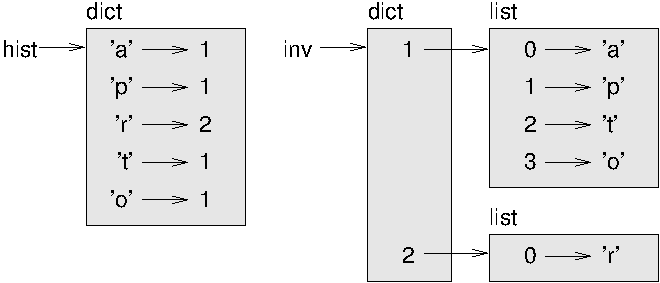
\includegraphics[scale=0.8]{figs/dict1.pdf}}
\caption{狀態圖.}
\label{fig.dict1}
\end{figure}

圖~\ref{fig.dict1} 是表示 {\tt hist}和 {\tt inverse}的狀態圖. 
字典用箱體表示, 其上有{\tt dict}類型標識, 其內是鍵值對. 
通常如果值是整數, 浮點數或者字符串, 我會將其繪製在箱體內部, 
但如果是串列, 我會繪製在箱體外部, 只是為了簡單易懂. 
\index{state diagram}
\index{diagram!state}

串列可以是字典的值, 就像圖中所示, 但是不能作為鍵使用. 
下面是擅自使用遇到的錯誤:
\index{TypeError}
\index{exception!TypeError}


\begin{verbatim}
>>> t = [1, 2, 3]
>>> d = dict()
>>> d[t] = 'oops'
Traceback (most recent call last):
  File "<stdin>", line 1, in ?
TypeError: list objects are unhashable
\end{verbatim}
%
以前我講過, 字典的實現基於雜湊表, 意味著其鍵必須是{\bf 可散列的}.
\index{hash function}
\index{hashable}

{\bf hash}是一個函數, 其接收任意值(任何類型), 然後返回一個整數. 
字典會用這些被稱為哈希值的整數, 對鍵值對進行存儲和查找. 
\index{immutability}

如果鍵不可變, 則一切正常. 
如果鍵像串列一樣可變, 那麼便不太妙了. 
比如, 你想創建個鍵值對, 
Python 計算鍵的哈希值, 並將其存儲於相應的位置. 
如果你修改了鍵, 然後再次計算哈希值, 那麼位置不同了. 
這時候, 相當於一個鍵對應了兩個不同的位置, 或者說, 你無法找到
某個鍵了. 總之, 字典不能正常使用了. 

這也就是鍵必須要可哈希的原因, 以及為何像串列一樣的可變類型不能用作鍵的
原因. 突破此限制的最簡單方法是使用元組, 這個在下一章節會學到. 

因為字典是可變的, 所以不能用作鍵, 
但是{\em 可以}用作值. 

\section{快取}
\label{memoize}

如果你已經學習了第~\ref{one.more.example}節的{\tt fibonacci}函數, 
你會發現, 隨著參數越大, 函數運行時間越長. 而且, 耗時增長的速度很快. 
\index{fibonacci function}
\index{function!fibonacci}

若想理解其原由, 參考圖~\ref{fig.fibonacci}, 此{\bf 調用圖}展示了當
{\tt n=4}時{\tt fibonacci} 函數的調用情況:
\begin{figure}
\centerline
{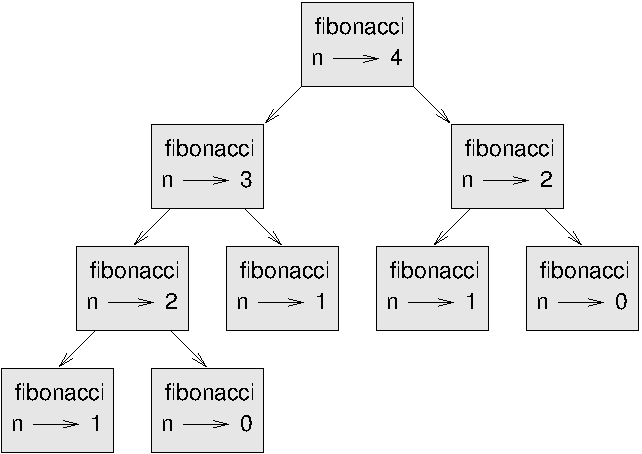
\includegraphics[scale=0.7]{figs/fibonacci.pdf}}
\caption{調用圖.}
\label{fig.fibonacci}
\end{figure}
調用圖是一堆函數框圖, 用框與框間的連線, 表示調用關係. 
此圖最頂層, 表示{\tt n=4}的{\tt fibonacci}函數會調用{\tt n=3}和{\tt n=2}時的函數. 
同樣, {\tt n=3}時的{\tt fibonacci}函數會調用{\tt n=2}和{\tt n=1}時的函數, 
以此類推. 
\index{function frame}
\index{frame}
\index{call graph}

算算 {\tt fibonacci(0)} 和 {\tt fibonacci(1)} 會被調用多少次吧. 
此操作是如此低效, 而且隨著參數變大, 效率更低. 
\index{memo}

另一種思路是跟蹤並記錄已經計算過的數據, 將其存儲到字典中. 
將之前計算過的值存儲起來, 方便後續使用, 這種操作叫做{\bf 快取}.
下面是 {\tt fibonacci}的``快取''版本:

\begin{verbatim}
known = {0:0, 1:1}

def fibonacci(n):
    if n in known:
        return known[n]

    res = fibonacci(n-1) + fibonacci(n-2)
    known[n] = res
    return res
\end{verbatim}
%
字典{\tt known} 用來跟蹤記錄過往結果. 
其初始包括兩項:0對應0, 1對應1.

每次{\tt fibonacci}被調用, 總會先檢查{\tt known}. 
如果結果已經存在, 則立刻返回結果. 否則, 計算結果, 
並保存到字典, 然後返回結果. 

當你運行這個版本的{\tt fibonacci}, 和以前版本相比, 
你會發現, 快了很多. 


\section{全局變量}
\index{global variable}
\index{variable!global}
上例中, {\tt known} 是在函數外創建, 
所以它屬於\verb"__main__"函數的框內, 這是一個特殊的框. 
\verb"__main__"函數中的變量, 有時也被認為是{\bf 全局的}, 
因為可以從任意函數訪問它們. 
不像局部變量, 其運行的函數一旦結束, 便會消失, 
全局變量可以在一個函數執行到另一個函數時, 也保持存在. 
\index{flag}
\index{main}

全局變量, 一個常用的地方, 便是作為{\bf 標識}使用;
也就是作為布爾變量, 來表示(``標識'')條件是否成立. 
比如, 有些程式會使用 {\tt verbose}作為標識, 來控制輸出信息的
詳細程度:

\begin{verbatim}
verbose = True

def example1():
    if verbose:
        print('Running example1')
\end{verbatim}
%
如果嘗試重新賦值全局變量, 可能會得到意外結果. 
下面的例子, 用全局變量來跟蹤函數是否被調用過:
\index{reassignment}

\begin{verbatim}
been_called = False

def example2():
    been_called = True         # WRONG
\end{verbatim}
%
運行此程式, 你會注意到\verb"been_called"的值沒有改變. 
問題在於 {\tt example2} 內部又創建了名為\verb"been_called"的局部變量. 
而局部變量會在函數結束後釋放, 並不會對全局變量產生影響. 
\index{global statement}
\index{statement!global}
\index{declaration}

如果想在函數內部修改全局變量, 你需要在賦值前, {\bf 聲明}這是全局變量:

\begin{verbatim}
been_called = False

def example2():
    global been_called 
    been_called = True
\end{verbatim}
%
這個{\bf global 聲明}會告訴解釋器,  ``在這個函數中, 當我說\verb"been_called", 
我指的是那個全局變量;而不是新建一個局部變量. ''
\index{update!global variable}
\index{global variable!update}

下面是段修改全局變量的代碼:

\begin{verbatim}
count = 0

def example3():
    count = count + 1          # WRONG
\end{verbatim}
%
運行後, 你會看到:
\index{UnboundLocalError}
\index{exception!UnboundLocalError}

\begin{verbatim}
UnboundLocalError: local variable 'count' referenced before assignment
\end{verbatim}
%
Python假設{\tt count}是局部的, 據此假設, 需要在更新變量前先讀取變量. 
解決方法依然是, 聲明{\tt count}為全局變量. 
\index{counter}

\begin{verbatim}
def example3():
    global count
    count += 1
\end{verbatim}
%
如果全局變量指向了可變的值, 那你在修改前, 無需聲明全局變量:
\index{mutability}

\begin{verbatim}
known = {0:0, 1:1}

def example4():
    known[2] = 1
\end{verbatim}
%
所以你可以在全局的串列或字典中, 添加, 移除以及替換元素, 
但是你若想對變量重新賦值, 需要提前聲明全局變量:

\begin{verbatim}
def example5():
    global known
    known = dict()
\end{verbatim}
%
全局變量是很有用, 但如果你到處使用, 並且還頻繁修改, 那麼程式往往會
難以調試. 


\section{調試}
\index{debugging}
隨著數據集越來越大, 僅僅使用打印輸出以及手工校驗結果的手段進行調試, 略顯不便. 
下面是調試大型數據集的一些建議:

\begin{description}

\item[降低輸入規模:] 如果可能, 降低數據集大小. 比如, 讀取文本文件, 
只讀取前10行, 或者使用你能找到的最簡樣例. 
可以重新編輯文件, 或者(更優的做法是)修改程式, 只讀取前{\tt n}行. 

如果報錯, 可以將{\tt n}減小為剛好會報錯的最小值, 
然後修正異常, 並逐步增大{\tt n}值, 如此迴圈往復. 

\item[檢驗概覽及類型:] 不要打印並檢驗全部數據集, 只需輸出數據的概覽:
比如, 字典中項的個數, 或者串列中數字總數量. 

值類型錯誤, 是產生運行時錯誤的常見原因. 
所以調試此類錯誤, 通常打印值的類型即可. 

\item[編寫自檢代碼:]  有時候, 你可以編寫代碼, 自動檢驗異常. 
例如, 你要計算數字串列的平均值, 你可以檢驗一下, 結果是否
比串列中最大值還要大, 或者比最小值還要小. 這叫做``合理性檢驗'', 
是因為要檢查結果是否``不合理''.  
\index{sanity check}
\index{consistency check}

另一種檢驗方法是比較兩種不同解法的結果, 看是否一致. 
這叫做``一致性檢驗''. 

\item[格式化輸出:] 格式化調試的輸出, 可以更直觀地展示錯誤. 
在第~\ref{factdebug}節, 我們曾展示過樣例. 另一個好用的工具是 {\tt pprint} 模塊, 
它提供了{\tt pprint}函數, 可以將內置類型輸出為更適合人類閱讀的格式({\tt pprint}
是``pretty pprint'' 的縮寫).
\index{pretty print}
\index{pprint module}
\index{module!pprint}

\end{description}

再次強調, 構建腳手架花費時間越長, 調試耗費時間越少. 
\index{scaffolding}


\section{術語表}

\begin{description}

\item[映射(mapping):] 集合中每個元素都對應到另一個集合的單一元素的關係.
\index{mapping}

\item[字典(dictionary):] 從鍵到相應的值的映射. 
\index{dictionary}

\item[鍵值對(key-value pair):] 鍵到值的映射關係的表示. 
\index{key-value pair}

\item[項(item):] 字典中, 鍵值對的別名. 
\index{item!dictionary}

\item[鍵(key):] 字典中的一個對象, 也是鍵值對的第一部分. 
\index{key}

\item[值(value):] 字典中的一個對象, 作為鍵值對的第二部分. 
這裡的表示和以前用到的``值''相比, 更加具體. 
\index{value}

\item[實現(implementation):] 一種執行計算的方式. 
\index{implementation}

\item[雜湊表(hashtable):] 實現Python字典的算法. 
\index{hashtable}

\item[哈希函數(hash function):] 雜湊表使用的函數, 用來計算鍵的位置. 
\index{hash function}

\item[散列的(hashable):] 一種可以使用哈希函數的類型. 
不可變類型, 像整型, 浮點型和字符串型, 都是可散列的;
像串列和字典這種可變類型, 則不是. 
\index{hashable}

\item[查找(lookup):] 一種字典操作, 根據鍵查找對應的值.
\index{lookup}

\item[反向查找(reverse lookup):] 一種字典操作, 通過值來查找對應的一個或多個鍵.
\index{reverse lookup}

\item[raise語句(raise statement):]  主動拋出異常的語句.
\index{raise statement}
\index{statement!raise}

\item[單元素集(singleton):] 只包含一個元素的串列(或者其他序列).
\index{singleton}

\item[調用圖(call graph):] 一種用來展示程式執行流程的圖, 包括每步創建的框, 
以及從調用者指向被調用者的箭頭. 
\index{call graph}
\index{diagram!call graph}

\item[備忘(memo):] 存儲計算過的值, 避免後續重複計算的操作. 
\index{memo}

\item[全局變量(global variable):] 定義在函數之外的變量. 
全局變量可以被任何函數獲取使用. 
\index{global variable}

\item[global語句(global statement):] 聲明變量是全局變量的語句.
\index{global statement}
\index{statement!global}

\item[標識(flag):] 標識條件是否為真的布爾變量. 
\index{flag}

\item[聲明(declaration):] 像{\tt global}一樣的語句, 用來告知解釋器
變量的有關信息. 
\index{declaration}

\end{description}


\section{習題集}

\begin{exercise}
\label{wordlist2}
\index{set membership}
\index{membership!set}

編寫函數, 讀取{\tt words.txt}中的單詞, 
將其作為鍵存儲於字典中. 值是什麼無關緊要. 
然後便可以用{\tt in}運算子快速檢驗某個字符串是否在字典中. 

如果你做過習題~\ref{wordlist1}, 可以比較一下這種實現, 和串列的{\tt in}運算, 
以及二分查找相比, 速度如何. 

\end{exercise}


\begin{exercise}
\label{setdefault}
閱讀字典方法 {\tt setdefault}的文檔, 
以此精簡\verb"invert_dict"版本. 
參見: \url{http://thinkpython2.com/code/invert_dict.py}.
\index{setdefault method}
\index{method!setdefault}

\end{exercise}


\begin{exercise}
用快取的方式重寫習題~\ref{ackermann} 中的Ackermann函數, 
看看是否快取方式可以使其處理較大參數. 
提示: 不能.
參考: \url{http://thinkpython2.com/code/ackermann_memo.py}.
\index{Ackermann function}
\index{function!ack}

\end{exercise}


\begin{exercise}
\index{duplicate}
如果做過習題~\ref{duplicate}, 你應該已經寫過一個\verb"has_duplicates" 函數, 
令其接收一個串列作為參數, 如果其中存在任意重複對象, 則返回{\tt True}.

使用字典來編寫一個更簡單高效的\verb"has_duplicates"版本. 
參考: \url{http://thinkpython2.com/code/has_duplicates.py}.
\end{exercise}


\begin{exercise}
\label{exrotatepairs}
\index{letter rotation}
\index{rotation!letters}

兩個單詞, 如果翻轉其中一個, 得到另一個, 則稱其為``翻轉詞組''
(參見習題~\ref{exrotate}中的\verb"rotate_word" ).

編寫程式讀取一個單詞表, 並找到所有的翻轉詞組. 
參考: \url{http://thinkpython2.com/code/rotate_pairs.py}.

\end{exercise}


\begin{exercise}
\index{Car Talk}
\index{Puzzler}

這是另一個來自{\em Car Talk}的謎題
(\url{http://www.cartalk.com/content/puzzlers}):

\begin{quote}
這個謎題來自於一個名為Dan O'Leary的朋友. 
他最近發現一個單音節, 五個字母的常用單詞, 其具有下述特徵. 
當你移除首字母, 剩下字母構成了一個和原單詞發音完全一樣的同音詞. 
如果再替換首字母, 也就是把首字母放回去, 移除第二個字母, 然後得到的又是
同音詞. 那麼問題來了, 這是什麼詞?

現在, 我給你展示一個錯誤的例子. 
咱們看一下這個五個字母的單詞, `wrack'.  W-R-A-C-K, 就是
`wrack with pain.' 中的那個`wrack'. 
如果移除首字母, 剩下四個字母的單詞, 'R-A-C-K.' 
比如, `Holy cow, did you see the rack on that buck!
It must have been a nine-pointer!' 發音完全一樣. 
如果你放回`w', 移除`r', 得到一個單詞, `wack', 
這是一個真正的單詞, 只是發音和前兩個不同. 

但是, 至少有一個這樣的單詞, Dan和我們都認識, 
分別刪除前兩個字母, 構成兩個新的四個字母單詞, 發音完全相同. 
問題是, 這個詞是什麼?
\end{quote}
\index{homophone}
\index{reducible word}
\index{word, reducible}

你可以用習題~\ref{wordlist2} 中的字典來檢驗一個字符串是否在單詞表中. 

若想檢查兩個單詞是否是同音詞, 可以用CMU發音詞典. 
這個詞典可以從\url{http://www.speech.cs.cmu.edu/cgi-bin/cmudict}
或\url{http://thinkpython2.com/code/c06d}下載. 
或者下載\url{http://thinkpython2.com/code/pronounce.py}代碼, 
這個文件提供了一個 \verb"read_dictionary"函數, 
可以讀取發音詞典並返回一個Python字典, 此字典將每個單詞映射到了
表示發音的字符串. 

編寫程式列出所有滿足謎語條件的單詞. 
答案: \url{http://thinkpython2.com/code/homophone.py}.

\end{exercise}



\chapter{元組}
\label{tuplechap}

本章介紹另一種內置類型, 元組, 以及串列、字典和元組如何一起使用. 
同時展示可變長度參數串列的一個特性, 以及聚合和擴展運算子. 

話外音:對於 ``tuple''如何發音, 尚無共識. 有人讀``tuh-ple'', 
和 ``supple''發音類系. 
但在編程領域, 多數人讀``too-ple'', 和``quadruple''發音一樣. 


\section{元組不可變}
\index{tuple}
\index{type!tuple}
\index{sequence}

元組也是值的序列. 其中值可以是任意類型, 也是用整數作為索引, 
所以在某些方面, 元組和串列很像. 
但兩者最大的區別在於元組不可變. 
\index{mutability}
\index{immutability}

從語法來看, 元組就是一個逗號分隔的序列:

\begin{verbatim}
>>> t = 'a', 'b', 'c', 'd', 'e'
\end{verbatim}
%
雖然不是很必要, 但一般都用括號把元組括起來:
\index{parentheses!tuples in}

\begin{verbatim}
>>> t = ('a', 'b', 'c', 'd', 'e')
\end{verbatim}
%
若要創建一個單元素的元組, 需要在末尾加上逗號:
\index{singleton}
\index{tuple!singleton}

\begin{verbatim}
>>> t1 = 'a',
>>> type(t1)
<class 'tuple'>
\end{verbatim}
%
括號中只有一個值, 便不是元組:

\begin{verbatim}
>>> t2 = ('a')
>>> type(t2)
<class 'str'>
\end{verbatim}
%
另一種創建元組的方法, 可以使用內置函數{\tt tuple}. 
如果不傳參數, 便會創建一個空元組:
\index{tuple function}
\index{function!tuple}

\begin{verbatim}
>>> t = tuple()
>>> t
()
\end{verbatim}
%
如果參數是一個序列(字符串, 串列或者元組), 
結果便會得到一個由元素序列構成的元組:

\begin{verbatim}
>>> t = tuple('lupins')
>>> t
('l', 'u', 'p', 'i', 'n', 's')
\end{verbatim}
%
因為{\tt tuple} 是一個內置函數名, 
所以要盡量避免用作變量名. 

多數串列運算子同樣適用於元組. 
所以用方括號也可以索引元組元素:
\index{bracket operator}
\index{operator!bracket}

\begin{verbatim}
>>> t = ('a', 'b', 'c', 'd', 'e')
>>> t[0]
'a'
\end{verbatim}
%
切片運算子也可以選擇元組中一段區間的元素. 
\index{slice operator}
\index{operator!slice}
\index{tuple!slice}
\index{slice!tuple}

\begin{verbatim}
>>> t[1:3]
('b', 'c')
\end{verbatim}
%
你如果想修改元組中的某個元素, 會報錯:
\index{exception!TypeError}
\index{TypeError}
\index{item assignment}
\index{assignment!item}

\begin{verbatim}
>>> t[0] = 'A'
TypeError: object doesn't support item assignment
\end{verbatim}
%
因為元組不可變, 所以你不能修改其中元素. 
但是你可以用另一個元組替換當前元組:

\begin{verbatim}
>>> t = ('A',) + t[1:]
>>> t
('A', 'b', 'c', 'd', 'e')
\end{verbatim}
%
這個語句創建新元組, 然後用 {\tt t} 指向它. 

關係運算子也同樣適用於元組以及其他序列;
Python會從各自序列的首元素開始比較, 如果相等, 則比較下一個元素, 
以此類推, 直到找出不同元素. 
而後續元素便不再比較(即使後面元素更大). 
\index{comparison!tuple}
\index{tuple!comparison}

\begin{verbatim}
>>> (0, 1, 2) < (0, 3, 4)
True
>>> (0, 1, 2000000) < (0, 3, 4)
True
\end{verbatim}



\section{元組賦值}
\label{tuple.assignment}
\index{tuple!assignment}
\index{assignment!tuple}
\index{swap pattern}
\index{pattern!swap}
交換變量的值經常會用到. 
比較傳統的方法, 是使用中間變量. 
比如下面例子, 互換 {\tt a} 和 {\tt b}的值:

\begin{verbatim}
>>> temp = a
>>> a = b
>>> b = temp
\end{verbatim}
%
這種方法比較麻煩; 用{\bf 元組賦值}會優雅很多:

\begin{verbatim}
>>> a, b = b, a
\end{verbatim}
%
左側是個變量元組;右側是個表達式元組. 
每個值都會賦值給其對應的變量. 
右側的表達式在賦值操作前都會先計算. 

同時左側變量的數量必須要和右側值的數量一樣:
\index{exception!ValueError}
\index{ValueError}

\begin{verbatim}
>>> a, b = 1, 2, 3
ValueError: too many values to unpack
\end{verbatim}
%
也有更普遍的用法, 右側可以用各種類型的序列(字符串, 串列或者元組). 
例如, 將一個郵箱地址切分為用戶名和域名, 可以這麼寫:
\index{split method}
\index{method!split}
\index{email address}

\begin{verbatim}
>>> addr = 'monty@python.org'
>>> uname, domain = addr.split('@')
\end{verbatim}
%
{\tt split}的結果是一個兩元素的串列;
第一個元素賦值給了{\tt uname}, 第二個賦值給了{\tt domain}. 

\begin{verbatim}
>>> uname
'monty'
>>> domain
'python.org'
\end{verbatim}
%

\section{元組作為返回值}
\index{tuple}
\index{value!tuple}
\index{return value!tuple}
\index{function!tuple as return value}
嚴格來講, 函數只能返回一個值, 但是如果這個值是一個元組, 
效果便等同於返回了多個值. 
比如, 你要將兩個整數相除, 計算商和餘數, 先計算{\tt x//y} , 再
計算{\tt x\%y}, 略顯低效. 更好的方法是同時計算兩個值. 
\index{divmod}

內置函數 {\tt divmod} 會接收兩個參數, 返回一個包含兩個值的元組, 
商和餘數. 同時, 你也可以將結果存儲為元組:

\begin{verbatim}
>>> t = divmod(7, 3)
>>> t
(2, 1)
\end{verbatim}
%
或者用元組賦值分別存儲結果:
\index{tuple assignment}
\index{assignment!tuple}

\begin{verbatim}
>>> quot, rem = divmod(7, 3)
>>> quot
2
>>> rem
1
\end{verbatim}
%
下面是一個返回元組的函數:

\begin{verbatim}
def min_max(t):
    return min(t), max(t)
\end{verbatim}
%
{\tt max} 和 {\tt min} 都是內置函數,  用來從序列中尋找最大值和最小值. 
\verb"min_max"函數計算兩者, 然後將其作為元組返回. 
\index{max function}
\index{function!max}
\index{min function}
\index{function!min}


\section{變長參數即元組}
\label{gather}
\index{variable-length argument tuple}
\index{argument!variable-length tuple}
\index{gather}
\index{parameter!gather}
\index{argument!gather}
函數可以接收任意數量參數. 以{\tt *} 開頭的參數會{\bf 聚合}所有參數作為一個元組. 
比如, {\tt printall}會接收任意數量的參數, 並打印輸出:

\begin{verbatim}
def printall(*args):
    print(args)
\end{verbatim}
%
這個聚合參數可以隨意命名, 但是 {\tt args}更為人所熟知. 
下面的函數展示其效果:

\begin{verbatim}
>>> printall(1, 2.0, '3')
(1, 2.0, '3')
\end{verbatim}
%
聚合的對立面是{\bf 擴展}. 
如果你有一個值的序列, 想將其作為多個參數, 傳入函數, 那便可以使用{\tt *}運算子. 
比如, {\tt divmod}僅接收兩個參數; 如果傳入一個元組, 則運行異常:
\index{scatter}
\index{argument scatter}
\index{TypeError}
\index{exception!TypeError}

\begin{verbatim}
>>> t = (7, 3)
>>> divmod(t)
TypeError: divmod expected 2 arguments, got 1
\end{verbatim}
%
但如果你擴展了元組, 那便運行正常:

\begin{verbatim}
>>> divmod(*t)
(2, 1)
\end{verbatim}
%
很多內置函數都會用到變長參數元組. 
比如, {\tt max}和{\tt min}都可以接收任意數量的參數:
\index{max function}
\index{function!max}
\index{min function}
\index{function!min}

\begin{verbatim}
>>> max(1, 2, 3)
3
\end{verbatim}
%
但{\tt sum}函數不行.
\index{sum function}
\index{function!sum}

\begin{verbatim}
>>> sum(1, 2, 3)
TypeError: sum expected at most 2 arguments, got 3
\end{verbatim}
%
做個練習, 寫個函數 \verb"sum_all", 使其可以接收任意數量參數, 並返回總和. 


\section{串列和元組}
\index{zip function}
\index{function!zip}
{\tt zip}是個內置函數,  其接收兩個或者更多序列作為參數, 並交錯獲取其中元素. 
這個函數的名字表示其像拉鏈, 彷若兩排交錯的牙齒. 

下面的例子是壓縮一個字符串和一個串列:

\begin{verbatim}
>>> s = 'abc'
>>> t = [0, 1, 2]
>>> zip(s, t)
<zip object at 0x7f7d0a9e7c48>
\end{verbatim}
%
結果是個 {\bf zip 對象}, 用來疊代數值對. 
所以{\tt zip}常常用在{\tt for}迴圈內:

\begin{verbatim}
>>> for pair in zip(s, t):
...     print(pair)
...
('a', 0)
('b', 1)
('c', 2)
\end{verbatim}
%

zip對象是一種{\bf 疊代器}, 也就是一種用來疊代序列的對象. 
疊代器和串列在某些方面比較相似, 但與串列不同的是, 你不能從
疊代器中通過索引獲取元素. 
\index{iterator}

如果你想使用串列的運算子和方法, 可以用zip對象構建串列:

\begin{verbatim}
>>> list(zip(s, t))
[('a', 0), ('b', 1), ('c', 2)]
\end{verbatim}
%
串列中都是元組; 在這個例子中, 每個元組都包括
字符串中的一個字母, 以及串列中的相應元素. 
\index{list!of tuples}

若序列長度不同, 則結果長度取決於較短的那個序列. 

\begin{verbatim}
>>> list(zip('Anne', 'Elk'))
[('A', 'E'), ('n', 'l'), ('n', 'k')]
\end{verbatim}
%
可以在{\tt for}迴圈中使用元組賦值, 遍曆元組串列:
\index{traversal}
\index{tuple assignment}
\index{assignment!tuple}

\begin{verbatim}
t = [('a', 0), ('b', 1), ('c', 2)]
for letter, number in t:
    print(number, letter)
\end{verbatim}
%
每次迴圈, Python都會獲取串列中的下一個元組, 並將其元素分別
賦給 {\tt letter} 和 {\tt number}. 
迴圈的輸出如下:
\index{loop}

\begin{verbatim}
0 a
1 b
2 c
\end{verbatim}
%
如果結合 {\tt zip}, {\tt for} 和元組賦值, 那你便得到了一個同時
遍歷兩個(或多個)序列的利器. 比如, \verb"has_match" 接收兩個序列, 
{\tt t1} 和 {\tt t2}, 如果存在索引{\tt i}, 令{\tt t1[i] == t2[i]}成立, 
則返回 {\tt True}:
\index{for loop}

\begin{verbatim}
def has_match(t1, t2):
    for x, y in zip(t1, t2):
        if x == y:
            return True
    return False
\end{verbatim}
%
如果你需要遍歷序列元素以及其索引, 可以使用
內置函數{\tt enumerate}:
\index{traversal}
\index{enumerate function}
\index{function!enumerate}

\begin{verbatim}
for index, element in enumerate('abc'):
    print(index, element)
\end{verbatim}
%
 {\tt enumerate} 返回的結果是一個枚舉對象, 
會疊代一個值對序列;
每個值對包括索引(從0開始)和給定序列中的元素. 
此例輸出同樣如下:

\begin{verbatim}
0 a
1 b
2 c
\end{verbatim}
%
\index{iterator}
\index{object!enumerate}
\index{enumerate object}


\section{字典和元組}
\label{dictuple}
\index{dictionary}
\index{items method}
\index{method!items}
\index{key-value pair}

字典有個方法叫做{\tt items}, 其返回一個元組序列, 每個元組都是一個鍵值對.

\begin{verbatim}
>>> d = {'a':0, 'b':1, 'c':2}
>>> t = d.items()
>>> t
dict_items([('c', 2), ('a', 0), ('b', 1)])
\end{verbatim}
%
結果是個 \verb"dict_items" 對象, 是一個疊代鍵值對的疊代器. 
可以在 {\tt for} 中使用, 如下所示:
\index{iterator}

\begin{verbatim}
>>> for key, value in d.items():
...     print(key, value)
...
c 2
a 0
b 1
\end{verbatim}
%
如你所想, 字典中的項沒有特定順序. 

相反, 你也可以用一個元組串列, 初始化一個新字典: 
\index{dictionary!initialize}

\begin{verbatim}
>>> t = [('a', 0), ('c', 2), ('b', 1)]
>>> d = dict(t)
>>> d
{'a': 0, 'c': 2, 'b': 1}
\end{verbatim}

將{\tt dict}和{\tt zip}結合使用, 便產生了一種新建字典的簡潔方法:
\index{zip function!use with dict}

\begin{verbatim}
>>> d = dict(zip('abc', range(3)))
>>> d
{'a': 0, 'c': 2, 'b': 1}
\end{verbatim}
%
字典的{\tt update}方法也可以接收一個元組串列, 然後將其
作為鍵值對添加到已有字典中.
\index{update method}
\index{method!update}
\index{traverse!dictionary}
\index{dictionary!traversal}

使用元組作為字典的鍵, 很常見(主要是串列不能). 
比如, 電話簿會將姓氏-名字映射到電話號碼. 
假設我們定義了{\tt last}, {\tt first} 和 {\tt number}, 
便可以編寫如下:
\index{tuple!as key in dictionary}
\index{hashable}

\begin{verbatim}
directory[last, first] = number
\end{verbatim}
%
方括號中的表達式是個元組. 
可以用元組賦值語句來遍歷字典.
\index{tuple!in brackets}

\begin{verbatim}
for last, first in directory:
    print(first, last, directory[last,first])
\end{verbatim}
%
此迴圈會遍歷 {\tt directory}中的鍵, 也就是元組. 
同時會將元組中的元素賦值給{\tt last} 和 {\tt first}, 
然後輸出姓名以及對應的電話號碼. 

在狀態圖中展示元組有兩種方法. 
較詳細的版本會展示起索引和元素, 就像串列一樣. 
例如, 圖~\ref{fig.tuple1} 展示了元組 \verb"('Cleese', 'John')" .
\index{state diagram}
\index{diagram!state}

\begin{figure}
\centerline
{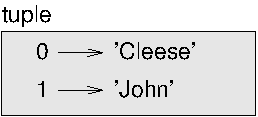
\includegraphics[scale=0.8]{figs/tuple1.pdf}}
\caption{狀態圖.}
\label{fig.tuple1}
\end{figure}

但在大規模得圖中, 你需要忽略細節. 
圖~\ref{fig.dict2}展示了電話簿的狀態.

\begin{figure}
\centerline
{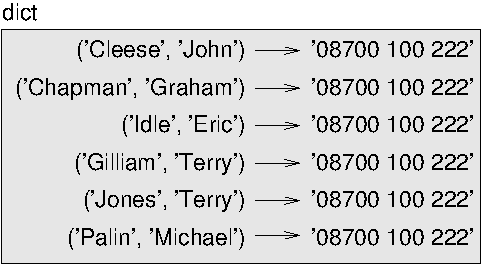
\includegraphics[scale=0.8]{figs/dict2.pdf}}
\caption{狀態圖.}
\label{fig.dict2}
\end{figure}

圖中的元組都使用Python語法形象表示. 
電話號碼是BBC的投訴熱線, 所以請不要撥打. 


\section{序列中的序列}
\index{sequence}

我一直講的是元組串列, 但是本章幾乎所有示例同樣適用於
串列構成的串列, 元組構成的元組, 以及串列構成的元組. 
為了避免枚舉各種組合, 直接叫做序列構成的序列, 便簡單多了. 

很多情形下, 不同類型的序列(字符串, 串列以及元組)可以替換使用, 
那你如何從中擇優呢?
\index{string}
\index{list}
\index{tuple}
\index{mutability}
\index{immutability}

從最顯而易見的情形考慮, 字符串比其他序列, 應用場景最有限, 
因為其元素需要是字符. 
同時, 他們不能被修改. 
如果你想要修改字符串中的字符(而不是新建一個新字符串), 
你最好還是用字符串列吧. 

串列比元組更加常用, 主要因為串列可變. 
但以下情況, 用元組會更好:

\begin{enumerate}

\item 在某些情形, 比如{\tt return}語句, 語法上創建元組比創建串列更簡便. 

\item 如果你想使用序列作為字典的鍵, 
你需要使用元組或者字符串這種不可變類型. 

\item 如果需要將一個序列作為參數傳遞給函數, 
使用元組可以有效降低使用別名帶來的潛在問題. 

\end{enumerate}

因為元組不可變, 所以它們不提供 {\tt sort} 和 {\tt reverse}這種修改現有串列的方法, 
但是Python提供內置函數 {\tt sorted}, 其接收任意序列, 然後返回一個排序後的新串列, 
也提供了{\tt reversed}函數, 其接收一個序列, 返回一個疊代器, 此疊代器可以
倒序遍歷串列. 
\index{sorted function}
\index{function!sorted} \index{reversed function}
\index{function!reversed}
\index{iterator}


\section{調試}
\index{debugging}
\index{data structure}
\index{shape error}
\index{error!shape}

串列, 字典以及元組都是 {\bf 資料結構}的例子;
本章我們開始了解複合資料結構, 像元組串列, 或者用元組作鍵, 
串列作值的字典. 
複合資料結構很有用, 但很容易產生我說的{\bf 格式異常};
就是當資料結構中出現了不恰當的類型, 大小或結構, 導致的錯誤. 
比如, 你想要一個含有一個整數的串列, 而我給了一個單純的整數
(不被串列包含), 那便會出錯. 
\index{structshape module}
\index{module!structshape}

為了調試這種異常, 我寫了一個叫作 {\tt structshape} 的模塊, 
其提供了一個{\tt structshape}函數, 可以接收任意資料結構作為參數, 
返回一個其格式的概述. 
你可以從 \url{http://thinkpython2.com/code/structshape.py} 下載. 

下面是一個簡單串列的示範:

\begin{verbatim}
>>> from structshape import structshape
>>> t = [1, 2, 3]
>>> structshape(t)
'list of 3 int'
\end{verbatim}
%

嚴謹點的寫法是``list of 3 int{\em s}'', 
但是忽略複數, 便於操作. 下面是一個串列構成的串列:

\begin{verbatim}
>>> t2 = [[1,2], [3,4], [5,6]]
>>> structshape(t2)
'list of 3 list of 2 int'
\end{verbatim}
%
如果串列中的元素類型不止一種, 
{\tt structshape} 按順序匯總類型:

\begin{verbatim}
>>> t3 = [1, 2, 3, 4.0, '5', '6', [7], [8], 9]
>>> structshape(t3)
'list of (3 int, float, 2 str, 2 list of int, int)'
\end{verbatim}
%
這是一個元組串列:

\begin{verbatim}
>>> s = 'abc'
>>> lt = list(zip(t, s))
>>> structshape(lt)
'list of 3 tuple of (int, str)'
\end{verbatim}
%
下面是一個包含3個項的字典, 每個項都是映射整數到字符串.

\begin{verbatim}
>>> d = dict(lt) 
>>> structshape(d)
'dict of 3 int->str'
\end{verbatim}
%
如果你對你的資料結構感到棘手, 可以試試{\tt structshape}.


\section{術語表}

\begin{description}

\item[元組(tuple):] 一個不可變的元素序列. 
\index{tuple}

\item[元組賦值(tuple assignment):] 一種序列居右, 變量元組在左的賦值語句. 
等號右側會先運算, 然後這些結果會賦值給相應的左側變量. 
\index{tuple assignment}
\index{assignment!tuple}

\item[聚合(gather):] 將多個參數聚合為一個元組的操作.
\index{gather}

\item[擴展(scatter):] 使序串列現為多個參數的操作. 
\index{scatter}

\item[zip對象(zip object):] 調用內置函數{\tt zip}返回的結果;
是可遍歷多個元組序列的對象. 
\index{zip object}
\index{object!zip}

\item[疊代器(iterator):] 可遍歷序列的對象, 但不適用串列運算子和方法. 
\index{iterator}

\item[資料結構(data structure):] 相關值的集合, 通常由串列, 字典, 元組等組成. 
\index{data structure}

\item[格式異常(shape error):] 值的格式不合適導致的錯誤, 通常是類型或者大小. 
\index{shape}

\end{description}


\section{習題集}

\begin{exercise}

編寫函數 \verb"most_frequent", 接收一個字符串, 然後按照字母頻數倒序輸出. 
從不同語言找一些文本素材, 看看不同語言之間字母頻數有何差異. 
並將結果與\url{http://en.wikipedia.org/wiki/Letter_frequencies}中的表格進行比較. 
參考:
\url{http://thinkpython2.com/code/most_frequent.py}.  
\index{letter frequency} 
\index{frequency!letter}

\end{exercise}


\begin{exercise}
\label{anagrams}
\index{anagram set}
\index{set!anagram}

再來些變位詞!

\begin{enumerate}

\item 編寫程式, 從文件中讀取單詞串列(參見第~\ref{wordlist}節), 
並且輸出所有的變位詞集合. 

下面是個輸出樣例:

\begin{verbatim}
['deltas', 'desalt', 'lasted', 'salted', 'slated', 'staled']
['retainers', 'ternaries']
['generating', 'greatening']
['resmelts', 'smelters', 'termless']
\end{verbatim}
%
提示: 你或許會想要構建個字典, 將字母集合映射到單詞串列, 
而串列中的單詞都可以用這些字母構成. 問題來了, 你如何表示這些字母集合, 
從而使其能夠作為鍵來使用?

\item 修改上面的程式, 使其先輸出最長的變位詞, 然後輸出次長, 依次類推. 
\index{Scrabble}
\index{bingo}

\item 拼字遊戲中, 你已有7張牌了, 如果又翻出了第8張, 構成了一個8字母的單詞, 那麼
你就獲得了一個``bingo''. 找找哪些8字母的組合, 是最可能獲得``bingo''的組合?

% (7, ['angriest', 'astringe', 'ganister', 'gantries', 'granites',
% 'ingrates', 'rangiest'])

參考: \url{http://thinkpython2.com/code/anagram_sets.py}.

\end{enumerate}
\end{exercise}

\begin{exercise}
\index{metathesis}
如果將一個單詞交換其中兩個字母的位置, 構成另一個單詞, 則這兩個單詞
構成了一個 ``易位詞對''; 比如, ``converse'' 和 ``conserve''.  
編寫程式, 從字典中尋找所有的``易位詞對''.
提示: 不用嘗試所有的單詞組合, 也不用嘗試所有可能易位操作. 
參考:
\url{http://thinkpython2.com/code/metathesis.py}.  
鳴謝: 這道題源自\url{http://puzzlers.org}上的一個例子. 
\end{exercise}


\begin{exercise}
\index{Car Talk}
\index{Puzzler}

這又是一個汽車廣播字迷
(\url{http://www.cartalk.com/content/puzzlers}):

\begin{quote}
每次從單詞中移除一個字母, 依然是正確的英文單詞, 這樣的單詞中, 
最長的是哪個?

可以從末尾或者中間移除字母, 但不能調整任何字母的順序. 
每次移除一個字母, 都得到一個新的英文單詞. 一直這樣操作, 
最終會得到一個字母, 同時這個字母也是一個英文單詞---可以在字典中找到. 
那麼最長的單詞是什麼, 以及它有多少個字母?

我舉個小例子: Sprite. 認識嗎? 從sprite開始, 從中間去掉一個字母, 移除r, 剩下的字母構成了單詞 spite, 
然後移除末尾的字母, 得到單詞 spit, 然後移除 s, 得到 pit, 然後依次得到 it, 和 I. 
\end{quote}
\index{reducible word}
\index{word, reducible}

編寫程式, 尋找所有這樣可以縮減的單詞, 然後確定最長的單詞. 

這道題相比其他題有些難, 所以這裡給些提示:

\begin{enumerate}

\item 你可能需要寫個函數, 接收一個單詞, 然後計算得到所有的單詞串列. 
這些單詞都是通過移除一個字母得到. 這些就是這個單詞的``子類''.
\index{recursive definition}
\index{definition!recursive}

\item 用遞歸思路來考慮, 如果一個單詞的子類是可以縮減的, 
那麼這個單詞就是可以縮減的. 可以將空字符串可縮減, 作為基準條件. 

\item 我提供的單詞串列 {\tt words.txt}, 不包含單字母單詞. 所以你可能需要添加``I'', ``a''和空字符串. 

\item 若想提升程式性能, 最好緩存住已知的可縮減單詞. 

\end{enumerate}

參考: \url{http://thinkpython2.com/code/reducible.py}.

\end{exercise}


%\begin{exercise}
%\url{http://en.wikipedia.org/wiki/Word_Ladder}
%\end{exercise}


\chapter{案例學習: 資料結構選擇}

截止當前, 你已學習了Python最核心的資料結構, 
同時也已熟悉了與之相關的一些算法. 
若想後續深入了解算法知識, 可以學習章節~\ref{algorithms}. 
但現在不用太急切; 後續時間方便了, 可以耐心學習. 

本章通過多道習題, 一個案例來讓你思考如何選擇和應用資料結構. 


\section{詞頻統計}
\label{analysis}

同往常一樣, 看答案前先盡量嘗試自己做一下. 

\begin{exercise}

寫個程式, 讀取文件, 把每行拆分成單詞, 去掉空格和標點, 並將其轉為小寫. 
\index{string module}
\index{module!string}

提示: {\tt string}模塊提供了名為{\tt whitespace}和名為 
{\tt  punctuation}的字符串, {\tt whitespace}包含了空格, 製表符, 換行等等; 而{\tt punctuation} 則包含各種標點符號. 
讓我們看看是否可以用Python來說明:

\begin{verbatim}
>>> import string
>>> string.punctuation
'!"#$%&\'()*+,-./:;<=>?@[\\]^_`{|}~'
\end{verbatim}
%
同時, 你可能會用到字符串方法{\tt strip},
{\tt replace} 和 {\tt translate}.
\index{strip method}
\index{method!strip}
\index{replace method}
\index{method!replace}
\index{translate method}
\index{method!translate}

\end{exercise}


\begin{exercise}
\index{Project Gutenberg}

前往Gutenberg項目 (\url{http://gutenberg.org}), 然後下載一個你最喜歡的書籍, 
要下載無版權書籍的純文本格式. 
\index{plain text}
\index{text!plain}

修改上個習題的代碼, 使其可以讀取所下載書籍的內容, 同時跳過書籍開頭部分的標題信息, 像以前一樣處理其餘單詞. 

調整代碼, 統計書中單詞總數, 以及每個單詞出現次數. 
\index{word frequency}
\index{frequency!word}

輸出書中不重複的單詞數量. 
比較不同作者在不同時代撰寫的不同書籍, 看看哪個作者的用詞最豐富?
\end{exercise}


\begin{exercise}

修改上面習題中的程式, 輸出書中出現次數最多的20個單詞. 

\end{exercise}


\begin{exercise}

修改上述代碼, 使其讀取單詞串列(參見第~\ref{wordlist}節), 
並輸出所有出現在書中, 但不在單詞表中的詞彙. 
看看有多少是拼寫異常? 又有多少是{\em 應該}包含在單詞表中的常用詞彙,
又有哪些是晦澀難懂的單詞?

\end{exercise}


\section{隨機數}
\index{random number}
\index{number, random}
\index{deterministic}
\index{pseudorandom}

多數程式, 給定同樣的輸入, 每次都是同樣的輸出, 這就叫做{\bf 確定性}.
確定性是件好事, 因為我們總是希望同樣的計算產生同樣的結果. 
但對於某些應用來說, 我們需要計算機能變得不可預測. 
遊戲就是一個很好的例子, 也有很多其他的應用場景. 

想讓一個程式完全隨機, 是很難的, 但是可以讓其看起來隨機. 
一種方法是使用算法生成{\bf 偽隨機}數.
偽隨機數不是真正隨機的, 因為它們是用一個確定的運算生成的, 
但只是從數字來看, 很難與真隨機進行區分. 
\index{random module}
\index{module!random}

{\tt random}模塊提供了生成偽隨機數(後續均用``隨機數''作為簡稱)的函數.
\index{random function}
\index{function!random}

函數{\tt random}會返回0.0到1.0之間(包括0.0但不包括1.0)的一個隨機浮點數. 
每次調用{\tt random}, 都會得到既定長序列上的下一個值. 
下面的迴圈便是一個例子:

\begin{verbatim}
import random

for i in range(10):
    x = random.random()
    print(x)
\end{verbatim}
%
函數{\tt randint}接收參數 {\tt low} 和{\tt high}, 
返回 {\tt low} 和 {\tt high} 之間的一個整數(包括兩者). 
\index{randint function}
\index{function!randint}

\begin{verbatim}
>>> random.randint(5, 10)
5
>>> random.randint(5, 10)
9
\end{verbatim}
%
若想從一個序列隨機選擇一個元素, 可以用{\tt choice}函數:
\index{choice function}
\index{function!choice}

\begin{verbatim}
>>> t = [1, 2, 3]
>>> random.choice(t)
2
>>> random.choice(t)
3
\end{verbatim}
%
{\tt random}模塊也提供了些可基於某種連續分布, 
比如高斯分布, 指數分布, 伽馬分布等, 生成隨機數的函數. 

\begin{exercise}
\index{histogram!random choice}

編寫\verb"choose_from_hist"函數, 使其
以第~\ref{histogram}節中定義的統計頻數為輸入, 然後從中
根據與頻數成正比的概率來返回一個隨機數. 
比如, 對於下面的頻數統計來說:

\begin{verbatim}
>>> t = ['a', 'a', 'b']
>>> hist = histogram(t)
>>> hist
{'a': 2, 'b': 1}
\end{verbatim}
%
你的函數應該返回\verb"'a'" 的概率是$2/3$,  返回\verb"'b'"的概率是$1/3$.
\end{exercise}


\section{詞頻}

繼續下面章節前, 先盡量完成上面的練習. 
你可以從 \url{http://thinkpython2.com/code/analyze_book1.py}下載
我的解決方案. 此外, 你也會需要\url{http://thinkpython2.com/code/emma.txt}這個文件.

下面是一個讀取文件, 並基於其中單詞構建詞頻統計的程式:
\index{histogram!word frequencies}

\begin{verbatim}
import string

def process_file(filename):
    hist = dict()
    fp = open(filename)
    for line in fp:
        process_line(line, hist)
    return hist

def process_line(line, hist):
    line = line.replace('-', ' ')
    
    for word in line.split():
        word = word.strip(string.punctuation + string.whitespace)
        word = word.lower()
        hist[word] = hist.get(word, 0) + 1

hist = process_file('emma.txt')
\end{verbatim}
%
這個程式會讀取 {\tt emma.txt}, 其中包括了Jane Austen的{\em Emma}小說. 
\index{Austen, Jane}

\verb"process_file" 遍歷文件中的每一行, 同時將每行內容逐次傳給\verb"process_line". 
詞頻{\tt hist} 在此處作為累加器使用. 
\index{accumulator!histogram}
\index{traversal}

\verb"process_line"用字符串方法{\tt replace}將連字符替換為空格, 然後用
 {\tt split}方法, 將整行拆分為字符串串列. 
然後遍歷串列, 並使用{\tt strip}方法, 移除標點符號, 使用{\tt lower}方法, 
轉換為全小寫. (此處簡單說是``轉換'', 但要記住字符串是不可變的, 所以像
{\tt strip}以及{\tt lower} 方法, 都是返回新的字符串.)

最終, \verb"process_line" 會通過新建項或者累加已有項, 更新詞頻統計.
\index{update!histogram}

若想統計文件中全部單詞數量, 可以將詞頻統計中的所有頻數相加求和即可:

\begin{verbatim}
def total_words(hist):
    return sum(hist.values())
\end{verbatim}
%
不同單詞的數量也就是字典中項的數量:

\begin{verbatim}
def different_words(hist):
    return len(hist)
\end{verbatim}
%
下面的代碼會輸出結果:

\begin{verbatim}
print('Total number of words:', total_words(hist))
print('Number of different words:', different_words(hist))
\end{verbatim}
%
結果如下:

\begin{verbatim}
Total number of words: 161080
Number of different words: 7214
\end{verbatim}
%

\section{最常用單詞}

若想找到最常用的單詞, 我們可以創建一個元組串列, 
每個元組都包含一個單詞和其頻數, 然後據此將串列排序.

下面函數接收一個詞頻統計, 然後返回一個詞-頻元組串列:

\begin{verbatim}
def most_common(hist):
    t = []
    for key, value in hist.items():
        t.append((value, key))

    t.sort(reverse=True)
    return t
\end{verbatim}

每個元組中, 頻數在前, 所以串列便是按頻數排序. 
下面迴圈會輸出前十個最常用單詞:

\begin{verbatim}
t = most_common(hist)
print('The most common words are:')
for freq, word in t[:10]:
    print(word, freq, sep='\t')
\end{verbatim}
%
此處使用用關鍵詞參數{\tt sep}, 來令{\tt print} 用換表符而不是空格作為``分隔符'', 
這樣第二列就會對齊.  下面是對{\em Emma}小說的統計結果:

\begin{verbatim}
The most common words are:
to      5242
the     5205
and     4897
of      4295
i       3191
a       3130
it      2529
her     2483
was     2400
she     2364
\end{verbatim}
%
上述代碼可以用 {\tt sort}函數的{\tt key}參數來簡化. 
如果你感興趣, 可以參閱 \url{https://wiki.python.org/moin/HowTo/Sorting}.


\section{可選參數}
\index{optional parameter}
\index{parameter!optional}
我們已經見到了諸多具有可選參數的內置函數和方法. 
而且我們也可以編寫具有可選參數的自定義函數. 
比如, 下面是輸出詞頻統計中最常用單詞的函數:
\index{programmer-defined function}
\index{function!programmer defined}

\begin{verbatim}
def print_most_common(hist, num=10):
    t = most_common(hist)
    print('The most common words are:')
    for freq, word in t[:num]:
        print(word, freq, sep='\t')
\end{verbatim}

第一個參數是不可或缺的; 第二個是可選的. 
{\tt num}的{\bf 默認值}是10.
\index{default value}
\index{value!default}

如果你只給定一個參數:

\begin{verbatim}
print_most_common(hist)
\end{verbatim}

{\tt num} 會使用默認值. 如果給定兩個參數:

\begin{verbatim}
print_most_common(hist, 20)
\end{verbatim}

{\tt num} 會使用實參來賦值. 
換句話說, 可選參數會{\bf 覆蓋} 默認值.
\index{override}

如果一個函數同時有必需和可選參數, 
則必需參數在前, 可選參數在後. 


\section{字典減法}
\label{dictsub}
\index{dictionary!subtraction}
\index{subtraction!dictionary}
從本書選擇不在{\tt words.txt} 中的單詞會比較麻煩, 你可能已經
意識到, 這是個集合減法; 也就是說, 我們希望找出所有在某集合
(本書單詞), 但不在另一個集合(單詞串列)中的單詞. 

{\tt subtract}函數會接收字典{\tt d1}和{\tt d2}, 返回一個新字典, 
其包含所有{\tt d1}中包含, 但{\tt d2}中不包含的鍵. 
因為我們不關心鍵的值, 所以就將其都設為None.

\begin{verbatim}
def subtract(d1, d2):
    res = dict()
    for key in d1:
        if key not in d2:
            res[key] = None
    return res
\end{verbatim}
%
若要找到包含在書中, 但是不包含在{\tt words.txt}中的單詞, 
我們可以用\verb"process_file" 函數先建立
一個{\tt words.txt}的詞頻統計, 然後再做減法:

\begin{verbatim}
words = process_file('words.txt')
diff = subtract(hist, words)

print("Words in the book that aren't in the word list:")
for word in diff:
    print(word, end=' ')
\end{verbatim}
%
下面是對 {\em Emma}小說 執行統計後的結果:

\begin{verbatim}
Words in the book that aren't in the word list:
rencontre jane's blanche woodhouses disingenuousness 
friend's venice apartment ...
\end{verbatim}
%
這些單詞有些是名字和所有格. 其他的, 例如``rencontre'', 已經很罕見了. 
但是有些依舊很常用, 確實也應該包含在串列中!

\begin{exercise}
\index{set}
\index{type!set}

Python提供了一種名為 {\tt set} 的資料結構, 其可以滿足多數的集合操作. 
你可以仔細閱讀章節~\ref{sets}, 或者閱讀
\url{http://docs.python.org/3/library/stdtypes.html#types-set}上面的文檔. 

編寫程式, 使用集合減法, 尋找包含在本書但是不在單詞串列中的單詞. 
參考:
\url{http://thinkpython2.com/code/analyze_book2.py}.

\end{exercise}


\section{隨機單詞}
\label{randomwords}
\index{histogram!random choice}

若要從詞頻統計中選擇隨機單詞, 最簡單的方法是每個單詞複製一定數量, 
複製的數量為其對應的頻數, 合併為串列, 然後, 從中選擇單詞:

\begin{verbatim}
def random_word(h):
    t = []
    for word, freq in h.items():
        t.extend([word] * freq)

    return random.choice(t)
\end{verbatim}
%
表達式{\tt [word] * freq}會將{\tt word}複製{\tt freq}份. 
{\tt extend}方法和{\tt append}作用相似, 只是前者參數是個序列. 

這個算法有效, 但不夠有效率; 每次選擇隨機單詞, 
都需要重新構建和原書一樣大的串列. 
顯然, 更優的方案是只建立一次串列, 然後多次選擇, 但串列依然很大.

一個更高效的方案是:

\begin{enumerate}

\item 使用 {\tt keys} 生成本書單詞的串列.

\item 用詞頻的各步累積之和(參看習題~\ref{cumulative}), 構建串列. 
串列中最後一項, 便是書中單詞總數, $n$. 
  
\item 選擇一個從1到$n$的隨機值. 使用二分搜索(參看習題~\ref{bisection}), 
尋找隨機值在累積值串列中所嵌入位置的索引. 

\item 使用該索引值從單詞串列中確定對應的單詞. 

\end{enumerate}

\begin{exercise}
\label{randhist}
\index{algorithm}

採用上面的算法, 編寫程式, 從書中隨機獲取單詞. 參考:
\url{http://thinkpython2.com/code/analyze_book3.py}.

\end{exercise}



\section{Markov分析}
\label{markov}
\index{Markov analysis}
如果從書中隨機選擇一些詞彙, 單詞意思可能都明白, 
但是你很難理解整句話:

\begin{verbatim}
this the small regard harriet which knightley's it most things
\end{verbatim}
%
一些單詞隨機組合, 很少能夠清楚表達意思, 因為其連續單詞之間
沒有聯繫. 比如, 一個完整的語句中, 我們知道``the''的後面往往緊跟著形容詞
或名詞, 很少是動詞或副詞. 

針對這些聯繫, 一種評估手段便是Markov分析, 這種方法的特徵在於對給定的單詞序列, 
評估接下來出現某個單詞的概率. 比如, 歌曲{\em Eric, the Half a Bee}的開頭:

\begin{quote}
Half a bee, philosophically, \\
Must, ipso facto, half not be. \\
But half the bee has got to be \\
Vis a vis, its entity. D'you see? \\
\\
But can a bee be said to be \\
Or not to be an entire bee \\
When half the bee is not a bee \\
Due to some ancient injury? \\
\end{quote}
%
這段文本中, ``half the''後邊總是緊跟著``bee'',
但是``the bee''後面有``has'' 也有 ``is''.
\index{prefix}
\index{suffix}
\index{mapping}

Markov 分析得到的結果, 一般是從每個前綴(比如``half the'' 和 ``the bee'')
到所有可能後綴(比如``has'' 和 ``is'')的映射.
\index{random text}
\index{text!random}
有了這個映射, 你便可以選擇任意單詞作為前綴, 
然後從可能的後綴中隨機選擇單詞. 繼而, 用合併後句子的末尾作為前綴, 與後綴拼接, 
構成下一個前綴, 不斷重複此過程. 

比如, 開始選擇``Half a''作為前綴, 然後緊跟著必然是``bee'', 
因為這個前綴只在文本中出現了一次. 然後, 下一次前綴便是``a bee'', 
其後綴則可能是``philosophically'', ``be'' 或 ``due''.

這個例子中, 前綴總是兩個單詞, 但你也可以用任意長度的前綴進行Markov分析. 

\begin{exercise}

Markov 分析:

\begin{enumerate}

\item 寫個程式, 讀取文本內容, 進行Markov分析. 
結果應該是個從前綴映射到可能後綴集合的字典. 
這個集合可以是串列, 元組或者字典; 取決於你的選擇. 
你可以用兩個詞的前綴測試程式, 但最好想辦法讓程式可以兼容其他長度的前綴. 

\item 在上面的程式中增加一個函數, 基於Markov分析生成隨機文本. 
下面是針對 {\em Emma}採用兩個單詞前綴進行Markov分析後, 生成的文本:

\begin{quote}
He was very clever, be it sweetness or be angry, ashamed or only
amused, at such a stroke. She had never thought of Hannah till you
were never meant for me?" "I cannot make speeches, Emma:" he soon cut
it all himself.
\end{quote}

這個例子中, 我保留了單詞的標點符號. 
結果看來語法正常, 但稍有瑕疵. 
從語義來看, 意思也能理解, 但不是很清晰明了. 

如果增加前綴單詞長度, 會如何? 得到的隨機文本是否會語義明了一些?

\item 一旦程式運行正常, 你可以試試混搭: 
如果將兩本或者多本書的文本合併, 生成的隨機文本夾雜著各處來源的單詞短語, 將非常有趣. 
\index{mash-up}

\end{enumerate}

鳴謝: 本案例參考了1999年由Addison-Wesley出版, Kernighan and Pike
所撰寫的{\em The Practice of Programming}一書中的例子. 
\end{exercise}

在繼續之前, 盡量嘗試一下解答此習題; 然後你可以從 
\url{http://thinkpython2.com/code/markov.py}下載我的方案, 同時, 
你也會用到\url{http://thinkpython2.com/code/emma.txt}.


\section{資料結構}
\index{data structure}

使用Markov方法生成隨機文本固然有趣, 但是這個練習有個關鍵點:
資料結構的選擇. 在解決前面的習題時, 你不得不考慮以下幾點:

\begin{itemize}

\item 如何表示前綴.

\item 如何表示可能的後綴集合.

\item 如何表示前綴和後綴集合的映射.

\end{itemize}

最後一個很簡單: 對於從鍵映射到相應的值, 很顯然, 採用字典. 

如果是前綴, 最好選擇字符串, 字符串串列或者字符串元組. 

對於後綴, 可以選擇串列; 或者詞頻統計(字典).
\index{implementation}

至於如何抉擇? 首先要考慮無論選擇哪種資料結構, 都不可避免的相應操作. 
對於前綴來說, 我們需要從開頭刪除單詞, 在末尾添加單詞. 比如, 如果現在
前綴是``Half a'', 後面的詞是``bee'',  你需要構建下一個前綴詞, ``a bee''. 
\index{tuple!as key in dictionary}

首選可能是串列, 因為很容易添加和刪除元素, 但我們同時需要
使用前綴作為字典的鍵, 所以串列不合適. 
而元組呢, 無法執行增刪操作, 
但是可以用加法運算子構建新元組:

\begin{verbatim}
def shift(prefix, word):
    return prefix[1:] + (word,)
\end{verbatim}
%

{\tt shift} 函數接收一個單詞元組, {\tt prefix}和一個字符串, 
{\tt word}, 取{\tt prefix}的除首位外的元素, 將{\tt word}拼接到
末尾, 構成新元組. 

對於後綴集合來說, 我們需要執行的操作包括增加新後綴(或者
增加已有後綴的頻次), 以及隨機選擇後綴. 

添加新後綴, 對於串列實現或者詞頻統計都同樣簡單. 
而從串列中選擇隨機元素很容易, 但是從一個詞頻字典中操作, 便不太高效
(參考習題~\ref{randhist}). 

目前來說, 我們考慮更多的是實現難易, 
但在選擇資料結構時, 還需要考慮一些其他因素. 
比如運行時間. 總有一些時候, 理論上可以預期某種資料結構就是比
另外一種要快. 比如, 我提到過的{\tt in}運算子, 字典比串列快, 
最起碼元素數量很多的時候, 一目了然. 

但往往你無法提前知曉哪種實現要更快. 一種方法是, 對每種資料結構都
進行實現, 然後運行比較, 看哪種更快. 這個方法叫做{\bf 基準分析}.
更實際一些的方法是選擇一種最容易實現的資料結構, 
然後看是否滿足預期. 如果滿足, 便沒必要優化了. 如果不滿足, 
可以使用一些工具, 像{\tt profile}模塊, 以定位程式最耗時的部分. 
\index{benchmarking}
\index{profile module}
\index{module!profile}

另一個需要考慮的因素是存儲空間. 
比如, 使用詞頻字典作為後綴集合, 只會消耗很少的空間, 
因為無論單詞在文中出現多少次, 每個單詞你只需存儲一次. 
某些情況下, 節省空間也可以提高程式運行速度, 而且在極端情況下, 
內存耗盡, 程式便無法運行. 但對於多數應用來說, 運行時間的考量要優先於存儲空間. 

最後再發散一下: 在本章節, 我已暗示, 我們應該使用一種資料結構進行分析和生成. 
但這二者又是兩個階段, 那麼便可以在分析時用一種資料結構, 然後在生成時, 
轉換為另一種資料結構. 如果生成節省的時間超過了轉換耗費的時間, 
那這種方案便有利可圖. 


\section{調試}
\index{debugging}

調試一個程式時, 尤其是面對嚴重問題時, 一定要做好以下五個步驟:

\begin{description}

\item[閱讀(Reading):] 檢查代碼, 讀給自己, 看看所寫是否符合所想. 

\item[運行(Running):] 做些修改, 運行各版本程式. 通常, 如果你在程式合適的位置, 
輸出合適的內容, 很容易定位問題, 不過有些時候, 你還是需要輔以腳手架代碼. 

\item[反思(Ruminating):] 花點時間多思考!是哪種錯誤: 語法, 運行時, 還是語義錯誤?
從異常信息, 或者程式輸出中能得到什麼信息? 哪種錯誤會引發你看到的問題?
問題出現前, 你最後一次改動了什麼?

\item[小黃鴨(Rubberducking):] 如果你向另一個人闡述問題, 有時候在問完問題之前, 
便找到了答案. 
通常, 你不需要找別人;你只需要對一個橡皮鴨喃喃自語. 
這便是眾所周知的{\bf 小黃鴨調試法}的來源. 這不是我瞎編的, 你可以
看\url{https://en.wikipedia.org/wiki/Rubber_duck_debugging}.

\item[回撤(Retreating):] 有時候, 最好的辦法是回退, 
取消最近的修改, 直到程式正常並且你能理解. 然後開始再次構建. 

\end{description}

新手程式師有時候會在以上某種步驟中徘徊, 而忘記了其他步驟. 
上面的每一步都有其不靈的時候. 
\index{typographical error}

比如, 遇到拼寫錯誤時, 閱讀代碼往往有效, 但如果是概念誤用, 那閱讀代碼便無濟於事了. 
如果你未理解代碼的功能, 那即使你閱讀100次, 也永遠不會發現錯誤, 
因為你理解的就有問題. 
\index{experimental debugging}

運行實例往往有用, 尤其是一些小而簡單的測試. 但是如果你不思考, 也不閱讀, 
便進行實驗, 那便會陷入我稱之為``隨機遊走編程''的誤區中, 
這種過程是隨機修改, 直至程式正常. 可想而知, 隨機遊走編程必然會耗費大量時間. 
\index{random walk programming}
\index{development plan!random walk programming}

你要多花時間思考. 
調試就像實驗科學. 
對於問題所在, 你至少要有一種假設. 
如果有兩種或者多種可能性, 想辦法設計個測試, 排除其中可能假設. 

但如果錯誤過多, 或者嘗試修復的程式過於龐大複雜, 
那即使再好的調試方案, 都會失效. 
有時候, 最好的選擇便是回退代碼, 簡化程式, 直到其正常且你能理解. 

新手程式師往往不願意回退代碼, 因為他們無法忍受刪除一行代碼(即使是錯誤代碼). 
可以在刪減代碼前, 將程式複製一份, 這樣會讓你感覺好一些. 
在你想還原的時候, 便可以一次性複製回來. 

定位嚴重的異常, 需要閱讀, 運行, 思考, 有時候還要回退代碼. 
如果在某個步驟卡殼了, 試試其他步驟. 


\section{術語表}

\begin{description}

\item[確定性(deterministic):] 給定相同輸入, 程式執行相同操作的特性. 
\index{deterministic}

\item[偽隨機數(pseudorandom):] 由確定算法生成, 只是看起來像是隨機的數字序列. 
\index{pseudorandom}

\item[默認值(default value):] 當可選參數未被賦值, 默認提供給可選參數的值. 
\index{default value}

\item[覆蓋(override):] 用參數替換默認值. 
\index{override}

\item[基準分析(benchmarking):] 在多個資料結構間抉擇的方法, 通過實現多個方案, 
並用可能的輸入作為樣本進行測試. 
\index{benchmarking}

\item[小黃鴨調試法(rubber duck debugging):] 通過對一個無生命對象, 比如小黃鴨, 闡述你的問題, 
從而調試的方法. 雖然小黃鴨不懂Python, 但是將問題描述清楚, 將有助於你解決問題. 
\index{rubber duck debugging}
\index{debugging!rubber duck}

\end{description}


\section{習題集}

\begin{exercise}
\index{word frequency}
\index{frequency!word}
\index{Zipf's law}

一個單詞的``排名''便是其在單詞串列中根據頻次排序後, 所在的位置:
最常用的排第一, 第二常用的排第二, 依次類推. 

Zipf定律(\url{http://en.wikipedia.org/wiki/Zipf's_law})
描述了自然語言中單詞排名和頻次的關係. 
具體來說, 其預測排名$r$的單詞的頻次$f$為:

\[ f = c r^{-s} \]
%
參數$s$和$c$取決於語言和文本. 
如果等式兩邊取對數, 得到:
\index{logarithm}

\[ \log f = \log c - s \log r \]
%
如果繪製log $f$和log $r$的關係圖, 你會得到一個斜率是$-s$, 截距為log $c$的斜線. 

編寫程式, 讀取文件中文本, 
統計單詞頻次, 按照頻次降序, 逐行輸出每個單詞, 以及
log $f$和log $r$. 
採用繪圖程式, 繪製結果曲線, 檢驗是否構成一條直線. 
能否再估計一下$s$的值?

參考: \url{http://thinkpython2.com/code/zipf.py}.
若要運行我的代碼, 需要繪圖模塊{\tt matplotlib}.
如果安裝了Anaconda, 默認是包括{\tt matplotlib}的;
否則, 你需要安裝一下. 
\index{matplotlib}

\end{exercise}



\chapter{文件}

本章介紹程式將數據保存在永久存儲中的``持久化''概念, 同時展示如何
使用不同類型的永久存儲, 比如文件和資料庫. 


\section{持久化}
\index{file}
\index{type!file}
\index{persistence}

以往我們遇到的多數程式都是一閃而過的, 因為它們運行很快, 也產生了一些輸出, 
但當運行結束, 其數據便會消失不見. 
如果再次運行, 又是從頭開始而已. 

有些程式是{\bf 持久化的}: 其運行時間很長(甚至一直運行);
這些程式至少會將部分數據進行永久儲存(比如, 硬盤);
如果程式中斷後重新運行, 便可以從之前停止的地方, 繼續執行. 

操作系統便是一個持久化程式的例子, 計算機一旦啟動, 便要執行諸多操作;
再比如網絡服務器, 需要一直運行, 等待接收來自網絡的請求. 

程式管理數據的一個最簡單方法是讀寫文本文件. 
之前, 我們已經接觸過讀取文本文件了, 
本章將學習如何使用程式, 將文本寫入文件. 

此外, 我們也可以將程式狀態存儲到資料庫中. 
本章將介紹一個簡單的資料庫, 以及模塊{\tt pickle}, 
它可以很容易存儲程式數據. 
\index{pickle module}
\index{module!pickle}


\section{讀和寫}
\index{file!reading and writing}

文本文件是存儲在永久介質, 比如硬盤, 閃存, 或光盤中的一系列字符. 
在第~\ref{wordlist}節, 我們已經學習了如何打開和讀取文件. 
\index{open function}
\index{function!open}

若要寫入文件, 需要在打開文件時, 用模式\verb"'w'"作為第二個參數:

\begin{verbatim}
>>> fout = open('output.txt', 'w')
\end{verbatim}
%
如果文件已存在, 採用寫入模式打開文件會清除原有內容, 重新寫入, 所以要格外謹慎!
如果文件不存在, 則會新建一個. 

{\tt open} 函數會返回一個文件對象, 此對象提供了各種操作文件的方法. 
{\tt write}方法可以將數據寫入文件. 

\begin{verbatim}
>>> line1 = "This here's the wattle,\n"
>>> fout.write(line1)
24
\end{verbatim}
%

返回值是已寫入的字符數量. 
文件對象會跟蹤其位置, 所以如果你再次調用{\tt write}方法, 
它會在文件末尾追加內容. 

\begin{verbatim}
>>> line2 = "the emblem of our land.\n"
>>> fout.write(line2)
24
\end{verbatim}
%
寫入完成, 需要關閉文件. 

\begin{verbatim}
>>> fout.close()
\end{verbatim}
%
\index{close method}
\index{method!close}
%
如果你沒有關閉文件, 程式運行結束, 便會自動關閉. 


\section{格式運算子}
\index{format operator}
\index{operator!format}

{\tt write}的參數需要是字符串, 所以, 若要向文件寫入其他類型, 
需要先轉換為字符串. 最簡單的方法是使用{\tt str}:

\begin{verbatim}
>>> x = 52
>>> fout.write(str(x))
\end{verbatim}
%
另一種方法是使用{\bf 格式運算子}, {\tt \%}. 
{\tt \%}在整數操作上是取余運算. 
但在第一個運算對象是字符串時, {\tt \%}便是格式運算子. 
\index{format string}

第一個運算對象通常是{\bf 格式字符串}, 它包括一個或者多個{\bf 格式序列}, 
而格式序列則是用來聲明第二個運算對象的輸出格式的. 
其運算結果便是字符串. 
\index{format sequence}

比如, 格式化序列 \verb"'%d'" 表示第二個運算對象
應該被格式化為一個十進制的整數字符串:

\begin{verbatim}
>>> camels = 42
>>> '%d' % camels
'42'
\end{verbatim}
%
結果為字符串\verb"'42'", 而不是整數{\tt 42}, 切勿混淆.

格式序列可以出現在字符串的任意位置, 所以你也可以在句子中
嵌入某個值:

\begin{verbatim}
>>> 'I have spotted %d camels.' % camels
'I have spotted 42 camels.'
\end{verbatim}
%
如果字符串中有不止一個格式序列, 那麼第二個參數必須是一個元組. 
每個格式序列依次對應元組中的元素. 

下面的例子中, 使用\verb"'%d'" 格式化整數, 
使用 \verb"'%g'" 格式化浮點數, 
使用\verb"'%s'" 格式化字符串:

\begin{verbatim}
>>> 'In %d years I have spotted %g %s.' % (3, 0.1, 'camels')
'In 3 years I have spotted 0.1 camels.'
\end{verbatim}
%
元組中元素數量要和字符串中格式序列的數量保持一致. 
同時, 元素的類型也要和格式序列保持一致:
\index{exception!TypeError}
\index{TypeError}

\begin{verbatim}
>>> '%d %d %d' % (1, 2)
TypeError: not enough arguments for format string
>>> '%d' % 'dollars'
TypeError: %d format: a number is required, not str
\end{verbatim}
%
在第一個例子中, 元素數量不一致;
第二個例子中, 元素類型不匹配.

可以從
\url{https://docs.python.org/3/library/stdtypes.html#printf-style-string-formatting}
了解更多關於格式運算子的信息. 
此外, 有個功能更強大的替代方案, 便是字符串的格式化方法, 你可以從
\url{https://docs.python.org/3/library/stdtypes.html#str.format}了解更多細節. 

% You can specify the number of digits as part of the format sequence.
% For example, the sequence \verb"'%8.2f'"
% formats a floating-point number to be 8 characters long, with
% 2 digits after the decimal point:

% % \begin{verbatim}
% >>> '%8.2f' % 3.14159
% '    3.14'
% \end{verbatim}
% \afterverb
% %
% The result takes up eight spaces with two
% digits after the decimal point.  


\section{文件名和路徑}
\label{paths}
\index{filename}
\index{path}
\index{directory}
\index{folder}

文件是按照{\bf 目錄}(也叫``文件夾'')來組織存放的. 
每個運行的程式都有一個``當前目錄'', 也是大多數運算的默認目錄. 
比如, 當你要打開一個文件讀取內容時, Python會在當前目錄尋找此文件. 
\index{os module}
\index{module!os}

{\tt os}模塊(``os'' 即 ``operating system'')提供了操作文件和目錄的函數. 
{\tt os.getcwd} 會返回當前目錄的名稱:
\index{getcwd function}
\index{function!getcwd}

\begin{verbatim}
>>> import os
>>> cwd = os.getcwd()
>>> cwd
'/home/dinsdale'
\end{verbatim}
%
{\tt cwd} 意為``current working directory'', 即 ``當前工作目錄''. 
本例中結果為{\tt /home/dinsdale}, 也就是用戶{\tt dinsdale}的主目錄. 
\index{working directory}
\index{directory!working}

像\verb"'/home/dinsdale'" 這樣表示文件或者目錄的字符串叫做{\bf 路徑}. 

一個簡單的文件名, 比如{\tt memo.txt} 也可以認為是一個路徑, 
只是, 這是一個{\bf 相對路徑}, 因為它和當前目錄相關. 
如果當前目錄是{\tt /home/dinsdale}, 那麼文件名{\tt memo.txt} 便
指的是 {\tt /home/dinsdale/memo.txt}這個路徑. 
\index{relative path} \index{path!relative}
\index{absolute path} \index{path!absolute}

以{\tt /} 開頭的路徑, 不依賴於當前目錄;
所以叫做{\bf 絕對路徑}.
若要找到一個文件的絕對路徑, 可以使用 {\tt os.path.abspath}:

\begin{verbatim}
>>> os.path.abspath('memo.txt')
'/home/dinsdale/memo.txt'
\end{verbatim}
%
{\tt os.path} 提供了處理文件名和路徑的其他一些方法. 
比如, {\tt os.path.exists}會檢查文件或目錄是否存在:
\index{exists function}
\index{function!exists}

\begin{verbatim}
>>> os.path.exists('memo.txt')
True
\end{verbatim}
%
如果存在, {\tt os.path.isdir}可以用來檢查其是否是一個目錄:

\begin{verbatim}
>>> os.path.isdir('memo.txt')
False
>>> os.path.isdir('/home/dinsdale')
True
\end{verbatim}
%
同理, {\tt os.path.isfile}可以判斷路徑是否是一個文件. 

{\tt os.listdir} 會返回指定目錄下的文件串列(以及其他目錄):

\begin{verbatim}
>>> os.listdir(cwd)
['music', 'photos', 'memo.txt']
\end{verbatim}
%
為了展示這些函數的用法, 下面的``walks''示例會遍歷一個目錄, 
輸出所有文件的名稱, 同時遞歸遍歷自己所有目錄. 
\index{walk, directory}
\index{directory!walk}

\begin{verbatim}
def walk(dirname):
    for name in os.listdir(dirname):
        path = os.path.join(dirname, name)

        if os.path.isfile(path):
            print(path)
        else:
            walk(path)
\end{verbatim}
%

{\tt os.path.join} 會接收一個目錄和一個文件名, 將其拼接為一個完整路徑. 

{\tt os} 模塊也提供了一個名為{\tt walk}的函數, 和上面例子相似, 但更通用. 
做個練習, 閱讀其文檔, 並使用此函數輸出給定目錄以及其子目錄下的所有文件的名稱. 
可以從\url{http://thinkpython2.com/code/walk.py}下載我的答案. 


\section{捕獲異常}
\label{catch}

當你讀寫文件時, 很多意外會發生. 
如果嘗試打開一個不存在的文件, 通常會得到{\tt FileNotFoundError}:
\index{open function}
\index{function!open}
\index{exception!IOError}
\index{IOError}

\begin{verbatim}
>>> fin = open('bad_file')
FileNotFoundError: [Errno 2] No such file or directory: 'bad_file'

\end{verbatim}
%
如果你沒有權限訪問文件, 也會異常:
\index{file!permission}
\index{permission, file}

\begin{verbatim}
>>> fout = open('/etc/passwd', 'w')
PermissionError: [Errno 13] Permission denied: '/etc/passwd'
\end{verbatim}
%
如果你嘗試打開一個目錄, 讀取內容, 會得到下面異常:

\begin{verbatim}
>>> fin = open('/home')
IsADirectoryError: [Errno 21] Is a directory: '/home'
\end{verbatim}
%
想要避免這些錯誤, 你可以使用 {\tt os.path.exists}和{\tt os.path.isfile} 這樣的函數, 
但是會耗費大量時間, 編寫大量代碼來檢驗各種可能(如果說``{\tt Errno 21}'' 代表什麼的話, 
那便是至少有21個異常會發生). 

\index{exception, catching}
\index{try statement}
\index{statement!try}

所以更好的做法是盡早嘗試, 盡快應對可能的異常, 而這恰恰是{\tt try}語句的作用. 
而其語法和{\tt if...else}語句很相似:

\begin{verbatim}
try:    
    fin = open('bad_file')
except:
    print('Something went wrong.')
\end{verbatim}
%
Python 會先執行{\tt try}語句區塊. 
如果一切正常, 會跳過{\tt except}語句, 繼續執行. 
如果異常發生, 會跳出{\tt try}語句塊, 執行{\tt except}語句塊. 

使用{\tt try}語句處理異常的方式叫做{\bf 捕獲}異常. 
在上面例子中, {\tt except}部分會輸出一句錯誤信息, 但幫助不大. 
通常, 捕獲異常是為了讓你有機會修正問題, 或重試程式, 或者至少優雅地結束程式. 


\section{資料庫}
\index{database}

{\bf 資料庫}是用來存儲數據的文件. 
很多資料庫都是像字典一樣構建, 從鍵映射到值, 進行數據存儲. 
資料庫和字典之間最大的區別, 在於資料庫存儲在磁盤(或者其他永久存儲中), 
所以程式結束後, 數據依然存在. 
\index{dbm module} \index{module!dbm}

 {\tt dbm} 模塊提供了一個創建和更新資料庫文件的介面. 
下面的例子中, 我將創建一個資料庫來存儲圖片文件的描述. 
\index{open function}
\index{function!open}

打開資料庫便如打開文件一樣:

\begin{verbatim}
>>> import dbm
>>> db = dbm.open('captions', 'c')
\end{verbatim}
%

模式 \verb"'c'" 表示如果資料庫不存在, 則新建一個. 
其結果是一個資料庫對象, 使用方式(很多操作)和字典一樣.
\index{database object}
\index{object!database}

當創建新的項, {\tt dbm}便會更新資料庫文件.
\index{update!database}

\begin{verbatim}
>>> db['cleese.png'] = 'Photo of John Cleese.'
\end{verbatim}
%
當想要讀取其中的項時,  {\tt dbm}如下讀取內容:

\begin{verbatim}
>>> db['cleese.png']
b'Photo of John Cleese.'
\end{verbatim}
%
結果是一個{\bf 字節對象}, 所以會用{\tt b}開頭. 
字節對象和字符串在很多地方很相似. 
隨著你對Python的理解不斷深入, 這種差異便需要引起重視, 但是目前為止, 
可以暫時忽視這些差異. 
\index{bytes object}
\index{object!bytes}

如果對一個已經存在的鍵重新賦值, {\tt dbm}會替換舊值:

\begin{verbatim}
>>> db['cleese.png'] = 'Photo of John Cleese doing a silly walk.'
>>> db['cleese.png']
b'Photo of John Cleese doing a silly walk.'
\end{verbatim}
%

字典的某些方法, 比如{\tt keys} 和 {\tt items}, 
並不適用於資料庫對象. 但是可以用{\tt for}迴圈對其進行疊代, 遍歷對象:
\index{dictionary methods!dbm module}

\begin{verbatim}
for key in db:
    print(key, db[key])
\end{verbatim}
%
和操作其他文件一樣, 用完之後, 需要關閉資料庫:

\begin{verbatim}
>>> db.close()
\end{verbatim}
%
\index{close method}
\index{method!close}


\section{序列化}
\index{pickling}

{\tt dbm}的一個限制是, 鍵和值必須是字符串或者字節. 
如果使用其他類型, 會報錯. 
\index{pickle module} \index{module!pickle}

這時候{\tt pickle}模塊便有用武之地了. 
它可以將幾乎任何類型對象轉換為字符串, 以便存儲於資料庫中, 
然後用的時候再將字符串轉換回對象. 

{\tt pickle.dumps}會接收一個對象參數, 返回一個字符串形式的文本
({\tt dumps}是``dump string''的縮寫):

\begin{verbatim}
>>> import pickle
>>> t = [1, 2, 3]
>>> pickle.dumps(t)
b'\x80\x03]q\x00(K\x01K\x02K\x03e.'
\end{verbatim}
%

這個格式明顯不適合人類閱讀; 但是對於{\tt pickle}模塊, 卻容易解碼. 
{\tt pickle.loads}(``load string'')可以將編碼後的結果重新翻譯回來:

\begin{verbatim}
>>> t1 = [1, 2, 3]
>>> s = pickle.dumps(t1)
>>> t2 = pickle.loads(s)
>>> t2
[1, 2, 3]
\end{verbatim}
%
雖然新舊對像的值一樣, 但(通常)不是同一個對象:

\begin{verbatim}
>>> t1 == t2
True
>>> t1 is t2
False
\end{verbatim}
%
換個說法, 序列化對象, 然後再反序列化的過程, 就如同複製對象一樣. 

你可以用{\tt pickle}來將任何非字符串數據存儲到資料庫中. 
實際上, 因為這種聯動操作過於普遍, 以至於將其
封裝進了{\tt shelve}模塊.  
\index{shelve module}
\index{module!shelve}


\section{管道}
\index{shell}
\index{pipe}

多數操作系統都提供了命令行介面, 一般稱為 {\bf shell}.
Shells 通常提供了大量命令, 以定位文件系統, 以及運行應用. 
比如, 在Unix中, 你可以用{\tt cd}命令切換目錄, 
使用{\tt ls}命令顯示目錄下的內容, 以及(比如)鍵入{\tt firefox} 來啟動瀏覽器. 
\index{ls (Unix command)}
\index{Unix command!ls}

任何你能通過shell啟動的程式, 都可以通過Python, 使用{\bf 管道對象}來啟動, 這個對象表示了一個運行中的程式. 

比如, Unix命令{\tt ls -l}通常會用長文件名格式來顯示當前目錄內容. 
在Python中, 可以用{\tt os.popen}\footnote{{\tt popen}模塊目前已經廢棄, 
也就是說, 我們應該避免使用它, 而盡量使用{\tt subprocess}模塊. 
但因為{\tt subprocess}模塊相對更複雜, 為了簡便, 
暫時用{\tt popen}模塊來講解, 直到確實不能用再說} 來運行{\tt ls}:
\index{popen function}
\index{function!popen}

\begin{verbatim}
>>> cmd = 'ls -l'
>>> fp = os.popen(cmd)
\end{verbatim}
%
參數是個包含shell命令的字符串. 
返回值是一個對象, 使用方式和打開的文件對象一樣. 
你可以用{\tt readline} 來逐行獲取{\tt ls}進程的輸出, 
或者用{\tt read}來一次獲取全部內容:
\index{readline method}
\index{method!readline}
\index{read method}
\index{method!read}

\begin{verbatim}
>>> res = fp.read()
\end{verbatim}
%
當讀取結束, 和操作文件一樣, 需要關閉通道:
\index{close method}
\index{method!close}

\begin{verbatim}
>>> stat = fp.close()
>>> print(stat)
None
\end{verbatim}
%
返回值是{\tt ls}進程的最終狀態;
{\tt None}表示正常結束(沒有錯誤).

比如, 多數Unix系統都提供了一個{\tt md5sum}命令, 
來讀取文件內容, 並計算一個``校驗值''. 
可以通過 \url{http://en.wikipedia.org/wiki/Md5}了解更多MD5的知識. 
這個命令提供了一種有效的方法, 可以檢驗兩個文件是否內容一樣. 
不同文件產生相同校驗值的概率極低(可以說, 在宇宙崩塌之前都不太可能). 
\index{md5}
\index{checksum}

你可以使用管道從Python中運行{\tt md5sum}, 並獲取結果:

\begin{verbatim}
>>> filename = 'book.tex'
>>> cmd = 'md5sum ' + filename
>>> fp = os.popen(cmd)
>>> res = fp.read()
>>> stat = fp.close()
>>> print(res)
1e0033f0ed0656636de0d75144ba32e0  book.tex
>>> print(stat)
None
\end{verbatim}



\section{編寫模塊}
\label{modules}
\index{module, writing}
\index{word count}
任何包含Python代碼的文件, 都可以作為模塊導入使用. 
例如, 假設你有一個名為{\tt wc.py}的文件, 文件包含以下代碼:

\begin{verbatim}
def linecount(filename):
    count = 0
    for line in open(filename):
        count += 1
    return count

print(linecount('wc.py'))
\end{verbatim}
%
如果運行程式, 代碼會讀取自身, 並輸出文件中內容的行數, 也就是7.
你也可以像下面這樣導入這個模塊:

\begin{verbatim}
>>> import wc
7
\end{verbatim}
%
現在你有一個模塊{\tt wc}了:
\index{module object}
\index{object!module}

\begin{verbatim}
>>> wc
<module 'wc' from 'wc.py'>
\end{verbatim}
%
同時, 模塊對象提供了\verb"linecount"函數:

\begin{verbatim}
>>> wc.linecount('wc.py')
7
\end{verbatim}
%
如此這般, 用Python來編寫模塊. 

此處稍有瑕疵的地方在於, 上面例子中, 導入模塊時, 
會運行最後一行的測試代碼. 
通常, 當你導入一個模塊, 只應定義新的函數, 而不應執行它們.
\index{import statement}
\index{statement!import}

如果需要將程式作為模塊導入, 通常遵循下面的寫法:

\begin{verbatim}
if __name__ == '__main__':
    print(linecount('wc.py'))
\end{verbatim}
%
\verb"__name__" 是一個內置變量, 程式一旦開始運行, 便被賦值. 
如果程式作為一個腳本運行, \verb"__name__"的值為\verb"'__main__'";
就像上面例子, 測試代碼便會執行. 
如果程式作為模塊導入, 那\verb"__name__"的值便不是\verb"'__main__'", 
那測試代碼不會執行. 
\index{name built-in variable}
\index{main}

做個練習, 將上面代碼寫入{\tt wc.py}文件中, 將其作為腳本, 直接運行. 
然後運行Python解釋器, 並{\tt import wc}. 
當作為模塊導入時, \verb"__name__"的值是什麼?

警告:如果你導入一個已經導入過的模塊, Python不會做任何操作. 
即使文件變了, Python也不會重新讀取文件. 
\index{module!reload}
\index{reload function}
\index{function!reload}

如果你想重載模塊, 可以使用內置函數{\tt reload}, 
但這個不太靠譜, 最安全的方法應該是重啟解釋器, 然後再次導入模塊. 

\section{調試}
\index{debugging}
\index{whitespace}

當讀寫文件時, 可能會遇到一些空白導致的問題. 
這些問題很難被發現, 因為空格, 製表符和換行符都是不可見的:

\begin{verbatim}
>>> s = '1 2\t 3\n 4'
>>> print(s)
1 2  3
 4
\end{verbatim}
\index{repr function}
\index{function!repr}
\index{string representation}

這時便用到了內置函數 {\tt repr} . 
這個函數可以接收任何對象作為參數, 返回對象的字符串表示. 
對於字符串來說, 它會將空白字符輸出為反斜槓序列:

\begin{verbatim}
>>> print(repr(s))
'1 2\t 3\n 4'
\end{verbatim}

這個對於調試來說, 非常有用. 

另一個你可能遇到的難題是, 不同的系統會用不同的字符表示行尾. 
有些系統用換行符\verb"\n"表示, 有些系統用返回字符 \verb"\r"表示. 
有的系統又兩者都用. 
如果在不同系統間移動文件, 這些不兼容的地方, 便是引發問題之處. 
\index{end of line character}

對於多數系統來說, 有諸多程式可以實現格式轉換. 
你可以在\url{http://en.wikipedia.org/wiki/Newline}上查找軟體
(以及閱讀此問題的更多細節). 
或者, 你也可以自己寫一個轉換工具. 


\section{術語表}

\begin{description}

\item[持久化(persistent):] 程式可以隨時執行, 同時至少將數據保存到永久存儲中. 
\index{persistence}

\item[格式運算子(format operator):] 一個操作符, {\tt \%}, 連接格式字符串和元組, 
生成一個將元組元素格式化為指定格式的字符串. 
\index{format operator}
\index{operator!format}

\item[格式字符串(format string):] 用於格式運算子的字符串, 內含格式序列.  
\index{format string}

\item[格式序列(format sequence):] 格式字符串中的字符序列, 
比如{\tt \%d}, 規定了值應被格式化為哪種格式.
\index{format sequence}

\item[文本文件(text file):] 保存在類似硬盤一樣永久存儲介質上的字符序列. 
\index{text file}

\item[目錄(directory):] 文件集合的名稱, 也被稱為文件夾.
\index{directory}

\item[路徑(path):] 定位文件的字符串. 
\index{path}

\item[相對路徑(relative path):] 從當前目錄開始的路徑. 
\index{relative path}

\item[絕對路徑(absolute path):] 從文件系統中的根目錄開始的路徑. 
\index{absolute path}

\item[捕獲異常(catch):] 使用 {\tt try} 和 {\tt except} 語句來防止異常中斷程式執行. 
\index{catch}

\item[資料庫(database):] 一個文件, 其內容以類似字典的鍵值對應的方式來管理. 
\index{database}

\item[字節對象(bytes object):] 和字符串相似的一種對象.
\index{bytes object}
\index{object!bytes}

\item[shell:] 一個程式, 允許用戶輸入命令, 然後通過啟動其他程式來執行命令. 
\index{shell}

\item[管道對象(pipe object):] 表示一個正在運行的程式的對象, 
允許Python程式運行命令並讀取結果.
\index{pipe object}
\index{object!pipe}

\end{description}


\section{習題集}

\begin{exercise}

編寫一個名為{\tt sed}的函數, 接收一個模式字符串, 一個替換字符串, 以及兩個文件名;
這個函數需要讀取第一個文件, 然後把內容寫入第二個文件(如果沒有, 需要創建).
如果文件中出現模式字符串, 則用替換字符串進行替換. 

如果在打開, 讀取, 寫入或者關閉文件過程中發生異常, 
你的程式需要捕獲異常, 輸出錯誤信息, 安全退出. 
參考: \url{http://thinkpython2.com/code/sed.py}.

\end{exercise}


\begin{exercise}
\index{anagram set}
\index{set!anagram}

如果你從 \url{http://thinkpython2.com/code/anagram_sets.py}下載了
習題~\ref{anagrams}的答案, 你會發現, 
其創建了一個字典, 將一個有序字母字符串映射到了一個單詞串列, 
串列中的單詞均由這些字母構成. 比如,
\verb"'opst'" 映射著串列
\verb"['opts', 'post', 'pots', 'spot', 'stop', 'tops']".

編寫一個模塊, 導入 \verb"anagram_sets"模塊並提供兩個新的
函數: \verb"store_anagrams"可以將字母異位詞字典存儲到``shelf''; 
\verb"read_anagrams"則可以查找單詞並返回它的字母異位詞串列. 
參考: \url{http://thinkpython2.com/code/anagram_db.py}.

\end{exercise}


\begin{exercise}
\label{checksum}
\index{MP3}

在一個極大的MP3文件集合中, 可能會有重複的歌曲, 可能存儲在不同目錄, 
或者保存的名字不同. 
這個練習的目標在於查找重複歌曲. 

\begin{enumerate}

\item 編寫一個程式, 搜索目錄, 並遞歸其所有子目錄, 
返回一個包括所有給定後綴 (比如 {\tt .mp3})的完整路徑的串列. 
提示: {\tt os.path}提供了一些有用函數, 可以用來處理文件和路徑名稱. 
\index{duplicate}
\index{MD5 algorithm}
\index{algorithm!MD5}
\index{checksum}

\item 若要識別重複文件, 可以用{\tt md5sum}來計算每個文件的``校驗值''. 
如果兩個文件的校驗值相同, 則可以認為其內容相同. 
\index{md5sum}

\item 可以用Unix命令{\tt diff}再次確認兩個文件是否相同. 
\index{diff}

\end{enumerate}

答案: \url{http://thinkpython2.com/code/find_duplicates.py}.

\end{exercise}


\chapter{類和對象}
\label{clobjects}

截至當前, 你應該已經知曉如何使用函陣列織代碼, 
如何使用內置類型管理數據. 
接下來要學習``面向對象編程''了, 
這種方式是通過自定義類型來管理代碼和數據的模式. 
面向對象編程是一個很大的主題; 需要花費數章, 才能講解清楚. 
\index{object-oriented programming}

本章代碼樣例可以從
\url{http://thinkpython2.com/code/Point1.py} 下載;
同時, 習題答案可以從
\url{http://thinkpython2.com/code/Point1_soln.py}下載.


\section{自定義類型}
\label{point}
\index{programmer-defined type}
\index{type!programmer-defined}

我們已經接觸過多種Python的內置類型;
現在, 我們來嘗試定義一種新的類型. 
舉例來說, 創建一個叫{\tt Point}的類型, 用於表示二維空間中的一個點. 
\index{point, mathematical}

在數學語言中, 通常用括號中逗號分隔的坐標來表示點. 
比如, $(0,0)$表示起點, $(x,y)$表示原點向右偏移$x$個單位, 
向上偏移$y$個單位. 

在Python中, 有幾種方式可以表示點:

\begin{itemize}

\item 我們可以將坐標分別保存在兩個變量中, {\tt x}和{\tt y}. 

\item 我們也可以將坐標作為串列或元組的元素進行存儲. 

\item 我們也可以創建一個新的類型, 用對象表示點. 

\end{itemize}
\index{representation}

構建一種新的類型, 相比其他選項, 要更複雜, 
但是, 稍後會展示出它的威力. 

這種自定義類型, 也叫做{\bf 類}. 
類的定義便如下這般:
\index{class}
\index{object!class}
\index{class definition}
\index{definition!class}

\begin{verbatim}
class Point:
    """Represents a point in 2-D space."""
\end{verbatim}
%
代碼頭表示這個新類叫做{\tt Point}. 
代碼體是一個文檔字符串, 用來描述類的用途. 
你可以在類定義內部, 定義變量和方法, 
稍後再來講解. 
\index{Point class}
\index{class!Point}
\index{docstring}

聲明一個名為{\tt Point}的類, 便構建了一個{\bf 類對象}

\begin{verbatim}
>>> Point
<class '__main__.Point'>
\end{verbatim}
%
因為 {\tt Point} 在頂層定義, 所以其``全名''是 \verb"__main__.Point".
\index{object!class}
\index{class object}

類對象就像是一個創建對象的工廠. 
要創建一個Point,  可以像調用函數一般, 調用{\tt Point}.

\begin{verbatim}
>>> blank = Point()
>>> blank
<__main__.Point object at 0xb7e9d3ac>
\end{verbatim}
%
返回值是一個Point對象的引用, 同時賦值給了{\tt blank}.  

創建一個新的對象, 叫做{\bf 實例化}, 
而這個對象便是類的一個{\bf 實例}. 
\index{instance}
\index{instantiation}

當你打印一個實例時, Python會告訴你該實例所屬的類, 以及存儲在內存
中的位置(前綴{\tt 0x} 表示其後的數字為十六進制).
\index{hexadecimal}

每個對象都是某個類的實例, 所以``對象''和``實例''可以互用. 
但是本章我用``實例''來指代我所談論的自定義類型. 


\section{屬性}
\label{attributes}
\index{instance attribute}
\index{attribute!instance}
\index{dot notation}
可以用點標法對實例進行賦值:

\begin{verbatim}
>>> blank.x = 3.0
>>> blank.y = 4.0
\end{verbatim}
%

這種語法類似於從模塊中選取變量, 比如{\tt math.pi}, 或者 {\tt string.whitespace}. 
但在此處, 我們是使用點標法對對象中特定元素進行賦值. 
這些元素叫做{\bf 屬性(attribute)}. 

作為名詞, ``AT-trib-ute'' 的重音在第一個音節, 而作為動詞,  則發音如``a-TRIB-ute''. 

圖~\ref{fig.point}是展示了上面賦值結果的狀態圖. 
這樣展示一個對象及其屬性的狀態圖, 也叫{\bf 對象圖}. 
\index{state diagram}
\index{diagram!state}
\index{object diagram}
\index{diagram!object}

\begin{figure}
\centerline
{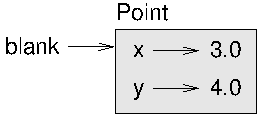
\includegraphics[scale=0.8]{figs/point.pdf}}
\caption{對象圖.}
\label{fig.point}
\end{figure}

變量{\tt blank}指向了一個包含兩個屬性的Point對象. 
每個屬性指向了一個浮點數. 

你可以基於同樣語法, 讀取屬性值:

\begin{verbatim}
>>> blank.y
4.0
>>> x = blank.x
>>> x
3.0
\end{verbatim}
%
表達式{\tt blank.x}表示, ``定位{\tt blank}指向的對象, 獲取{\tt x}的值.''
在上面例子中,  我們把這個表達式的值, 賦給了變量{\tt x}. 
變量{\tt x}和屬性{\tt x}並不會出現衝突. 

同時, 你也可以在任意表達式中使用點標法. 比如:

\begin{verbatim}
>>> '(%g, %g)' % (blank.x, blank.y)
'(3.0, 4.0)'
>>> distance = math.sqrt(blank.x**2 + blank.y**2)
>>> distance
5.0
\end{verbatim}
%
你也可以將實例作為參數使用. 比如:
\index{instance!as argument}

\begin{verbatim}
def print_point(p):
    print('(%g, %g)' % (p.x, p.y))
\end{verbatim}
%
\verb"print_point"會接收一個點對象作為參數, 並用數學符號來表示. 
若要調用, 可以將{\tt blank}作為參數傳入:

\begin{verbatim}
>>> print_point(blank)
(3.0, 4.0)
\end{verbatim}
%
在函數內部, {\tt p}是{\tt blank}的別稱, 所以如果函數改變了{\tt p}, 
那麼{\tt blank}也會發生變化. 
\index{aliasing}

做個練習, 寫個\verb"distance_between_points"函數, 
使其接收兩個Point對象作為參數, 返回兩者之間的距離. 



\section{矩形}
\label{rectangles}

有時設置對象的屬性很容易, 有時又很困難. 
假如你要設計一個類來表示矩形. 你會選擇什麼屬性來描述位置和大小?
暫時忽略角度, 假設矩形要麼垂直要麼水平, 從而簡化問題. 
\index{representation}

有兩種方案可選: 

\begin{itemize}

\item 你可以確定矩形的一個角(或者中心, 以及寬度和高度. 

\item 你也可以聲明兩個對角的位置. 

\end{itemize}

現在很難說哪種更優, 我們先實現第一種方案, 做個示例. 
\index{Rectangle class}
\index{class!Rectangle}

下面是類定義:

\begin{verbatim}
class Rectangle:
    """Represents a rectangle. 

    attributes: width, height, corner.
    """
\end{verbatim}
%
文檔字符串描述了相關屬性: {\tt width}和
{\tt height}是數字; {\tt corner} 是個Point對象, 表示左下角位置. 

要表示一個矩形, 首先要初始化一個Rectangle對象, 並給屬性賦值:

\begin{verbatim}
box = Rectangle()
box.width = 100.0
box.height = 200.0
box.corner = Point()
box.corner.x = 0.0
box.corner.y = 0.0
\end{verbatim}
%

表達式 {\tt box.corner.x}表示, 
``到{\tt box}指向的對象中, 選取名為{\tt corner}的屬性;
然後再到{\tt corner}指向對象中, 選取名為{\tt x}的屬性.''

\begin{figure}
\centerline
{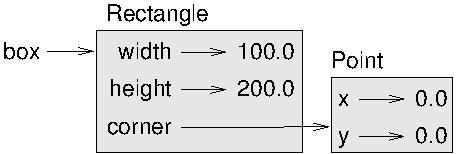
\includegraphics[scale=0.8]{figs/rectangle.pdf}}
\caption{對象圖.}
\label{fig.rectangle}
\end{figure}


圖~\ref{fig.rectangle} 展示了這個對象的狀態圖. 
一個對象作為另一個對象的屬性存在, 叫做{\bf 嵌套}. 
\index{state diagram}
\index{diagram!state}
\index{object diagram}
\index{diagram!object}
\index{embedded object}
\index{object!embedded}


\section{返回實例}
\index{instance!as return value}
\index{return value}

函數也可以返回實例. 比如, \verb"find_center" 可以接收一個
 {\tt Rectangle}參數, 返回一個包含{\tt Rectangle}的中心位置坐標的{\tt Point}實例:

\begin{verbatim}
def find_center(rect):
    p = Point()
    p.x = rect.corner.x + rect.width/2
    p.y = rect.corner.y + rect.height/2
    return p
\end{verbatim}
%
下面的例子中, 傳入了一個{\tt box}參數, 
然後將結果賦值給了{\tt center}變量:

\begin{verbatim}
>>> center = find_center(box)
>>> print_point(center)
(50, 100)
\end{verbatim}
%

\section{對象可變}
\index{object!mutable}
\index{mutability}

通過對屬性賦值, 可以改變對象的狀態. 
比如, 若要只改變矩形大小而不改變其位置, 可以只修改{\tt
width}和{\tt height}的值:

\begin{verbatim}
box.width = box.width + 50
box.height = box.height + 100
\end{verbatim}
%
你也可以通過函數, 修改對象. 例如, 
\verb"grow_rectangle" 函數會接收一個矩形對象和兩個數值, 
{\tt dwidth}和{\tt dheight}, 然後分別累加到矩形的寬和高上:

\begin{verbatim}
def grow_rectangle(rect, dwidth, dheight):
    rect.width += dwidth
    rect.height += dheight
\end{verbatim}
%
下面展示了其使用效果:

\begin{verbatim}
>>> box.width, box.height
(150.0, 300.0)
>>> grow_rectangle(box, 50, 100)
>>> box.width, box.height
(200.0, 400.0)
\end{verbatim}
%
在函數內部, {\tt rect}是{\tt box}的別名, 所以當函數修改了{\tt rect}的屬性, 
{\tt box}也會發生變化. 

做個練習, 編寫\verb"move_rectangle"函數, 使其接收一個矩形對象以及
{\tt dx}和{\tt dy}兩個值. 
同時對{\tt corner}的{\tt x}坐標加{\tt dx}, 
對{\tt corner}的{\tt y}坐標加上{\tt dy}, 
從而改變矩形的位置. 


\section{複製}
\label{copying}
\index{aliasing}

別名的使用會讓程式變得複雜, 因為一處改動可能會影響到其他地方. 
同時, 追蹤指向某個既定對象的所有變量, 又很困難. 
\index{copying objects}
\index{object!copying}
\index{copy module}
\index{module!copy}

所以, 常常用複製對象來代替別名使用. 
{\tt copy}模塊包含一個{\tt copy}函數, 可以複製任意對象:

\begin{verbatim}
>>> p1 = Point()
>>> p1.x = 3.0
>>> p1.y = 4.0

>>> import copy
>>> p2 = copy.copy(p1)
\end{verbatim}
%
{\tt p1}和{\tt p2}包含同樣的數據, 但它們不是同一個{\tt Point}對象.

\begin{verbatim}
>>> print_point(p1)
(3, 4)
>>> print_point(p2)
(3, 4)
>>> p1 is p2
False
>>> p1 == p2
False
\end{verbatim}
%

{\tt is}運算子表明{\tt p1}和{\tt p2}不是同一個對象, 這符合我們的預期. 
對於{\tt ==}, 本來我們看兩者包含數據一樣, 預期會是{\tt True}. 
但在此處, 令你沮喪的是, 對於實例來說, {\tt ==}運算子的默認操作和
{\tt is}運算子是一樣的; 都是檢驗對象是否相同, 而不是判斷是否相等.
這是因為對於用戶自定義類型, Python至少現在還無法知道如何衡量相等.
\index{is operator}
\index{operator!is}
\index{identity}
\index{equivalence}

如果你用 {\tt copy.copy}來複製一個矩形, 
會發現只複製了{\tt Rectangle}對象, 並沒有複製內嵌的{\tt Point}對象.
\index{embedded object!copying}

\begin{verbatim}
>>> box2 = copy.copy(box)
>>> box2 is box
False
>>> box2.corner is box.corner
True
\end{verbatim}

\begin{figure}
\centerline
{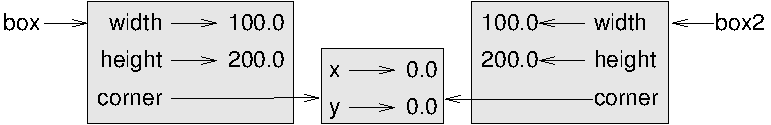
\includegraphics[scale=0.8]{figs/rectangle2.pdf}}
\caption{對象圖.}
\label{fig.rectangle2}
\end{figure}

圖~\ref{fig.rectangle2}展示了上面程式的對象圖.
\index{state diagram}
\index{diagram!state}
\index{object diagram}
\index{diagram!object}
這種操作叫做{\bf 淺拷貝}, 因為僅僅複製對象和其內部引用, 而不會複製內嵌對象. 
\index{shallow copy}
\index{copy!shallow}

多數應用中, 我們所希望的並不是這個效果. 
在這個例子中, 對其中一個執行 \verb"grow_rectangle" 函數操作, 
並不會影響另一個, 但對任何一個調用 \verb"move_rectangle"函數, 兩者都會被影響!
這種行為令人迷惑, 也更容易使人犯錯. 
\index{deep copy}
\index{copy!deep}

幸運的是,  {\tt copy} 模塊提供了一個{\tt
deepcopy}方法, 不僅複製對象, 同時也會複製其引用的對象, 
以及其引用對象內部引用的對象, 等等. 
所以, 你可以毫不意外地稱其為{\bf 深拷貝}. 
\index{deepcopy function}
\index{function!deepcopy}

\begin{verbatim}
>>> box3 = copy.deepcopy(box)
>>> box3 is box
False
>>> box3.corner is box.corner
False
\end{verbatim}
%
{\tt box3}和{\tt box} 是完全隔離的對象了. 

做個練習, 編寫一個 \verb"move_rectangle"新版本, 
使其創建並返回新的矩形對象, 而不是修改傳入的對象. 

\section{調試}
\label{hasattr}
\index{debugging}

當你開始使用對象時, 極有可能遇到新的異常. 
如果試圖讀取一個不存在的屬性, 會遇到屬性異常{\tt AttributeError}:
\index{exception!AttributeError}
\index{AttributeError}

\begin{verbatim}
>>> p = Point()
>>> p.x = 3
>>> p.y = 4
>>> p.z
AttributeError: Point instance has no attribute 'z'
\end{verbatim}
%
如若不確定對象類型, 可以如下這般查看:
\index{type function}
\index{function!type}

\begin{verbatim}
>>> type(p)
<class '__main__.Point'>
\end{verbatim}
%
你也可以使用{\tt isinstance}來判斷對象是否是某個類的實例:
\index{isinstance function}
\index{function!isinstance}

\begin{verbatim}
>>> isinstance(p, Point)
True
\end{verbatim}
%
如果你不確定對象是否存在某個屬性, 
可以用內置函數{\tt hasattr}, 進行判斷:
\index{hasattr function}
\index{function!hasattr}

\begin{verbatim}
>>> hasattr(p, 'x')
True
>>> hasattr(p, 'z')
False
\end{verbatim}
%
第一個參數可以是任意對象;
第二參數是個{\em 字符串}, 也就是某個屬性的名稱. 
\index{attribute}

你也可以用{\tt try}語句, 來判斷對象是否具有你所要的屬性:
\index{try statement}
\index{statement!try}

\begin{verbatim}
try:
    x = p.x
except AttributeError:
    x = 0
\end{verbatim}

這種方法便於編寫適用不同情況的函數;
更多相關話題在第~\ref{polymorphism}節會詳述. 


\section{術語表}

\begin{description}

\item[類(class):] 用戶自定義類型. 一個類的聲明會創建一個新的類對象. 
\index{class}
\index{programmer-defined type}
\index{type!programmer-defined}

\item[類對象(class object):] 包含自定義類型信息的對象. 
類對象可用來創建類的實例. 
\index{class object}
\index{object!class}

\item[實例(instance):] 屬於某個類的對象. 
\index{instance}

\item[初始化(instantiate):] 創建一個新對象.
\index{instantiate}

\item[屬性(attribute):] 一種與對象關聯的命名值. 
\index{attribute!instance}
\index{instance attribute}

\item[內嵌對象(embedded object):] 作為屬性存在於另一個對象內的對象. 
\index{embedded object}
\index{object!embedded}

\item[淺拷貝(shallow copy):] 複製對象的內容, 以及內嵌對象的所有引用;
通過{\tt copy}模塊中的{\tt copy}函數實現. 
\index{shallow copy}

\item[深拷貝(deep copy):] 複製對象內容以及所有內嵌對象, 以及內嵌對象的內嵌對象, 等等;
通過{\tt copy} 模塊的{\tt deepcopy}函數實現. 
\index{deep copy}

\item[對象圖(object diagram):] 展示對象, 及其屬性, 和屬性值的圖. 
\index{object diagram}
\index{diagram!object}

\end{description}


\section{習題集}

\begin{exercise}

定義一個名為 {\tt Circle}的類, 包含屬性{\tt center}和{\tt radius}, 
 {\tt center}是一個Point對象, {\tt radius}是一個數字. 

初始化一個{\tt Circle}對象, 用來表示一個圓, 其圓心為$(150, 100)$, 
半徑為 75.

編寫\verb"point_in_circle" 函數, 以Circle和Point為入參, 
如果Point 在圓內或者圓周上, 則返回True. 

編寫\verb"rect_in_circle"函數, 傳入一個Circle和一個Rectangle, 
如果Rectangle 完全處於圓內或圓周上, 則返回True. 

編寫函數\verb"rect_circle_overlap", 接收一個Circle和一個Rectangle, 
如果Rectangle的任意一個頂點在圓內, 則返回True. 
或者寫個更有挑戰性的版本, 如果矩形有任意部分在圓內, 則返回True. 

參考答案: \url{http://thinkpython2.com/code/Circle.py}.

\end{exercise}


\begin{exercise}

編寫函數\verb"draw_rect", 接收一個Turtle對象和一個Rectangle, 
用Turtle 繪製Rectangle. 
可以參考第~\ref{turtlechap}節的Turtle對象的使用示例. 

編寫函數\verb"draw_circle",  接收一個Turtle對象和一個Circle對象, 並繪製Circle.


參考答案: \url{http://thinkpython2.com/code/draw.py}.

\end{exercise}



\chapter{類和函數}
\label{time}

目前, 我們已經知道了如何創建新的類型, 下一步, 我們學習如何用
自定義類型對象作為參數和返回值, 編寫函數. 
本章將介紹``函數式編程模式'', 以及兩種新的程式開發範式. 


本章的代碼樣例可以從\url{http://thinkpython2.com/code/Time1.py}下載. 
習題答案可以參考
\url{http://thinkpython2.com/code/Time1_soln.py}.


\section{時間}
\label{isafter}

下面是一個自定義類型的示例, 我們定義了一個{\tt Time}類, 
用來記錄一天的時間. 
類的定義如下: 
\index{programmer-defined type}
\index{type!programmer-defined} 
\index{Time class} \index{class!Time}

\begin{verbatim}
class Time:
    """Represents the time of day.
       
    attributes: hour, minute, second
    """
\end{verbatim}
%
我們可以創建一個新的{\tt Time}對象, 
對時分秒分別定義屬性並賦值:

\begin{verbatim}
time = Time()
time.hour = 11
time.minute = 59
time.second = 30
\end{verbatim}
%
{\tt Time}對象的狀態圖如圖~\ref{fig.time}所示.
\index{state diagram}
\index{diagram!state}
\index{object diagram}
\index{diagram!object}

做個練習, 編寫\verb"print_time"函數, 令其接收一個Time對象, 並按照
{\tt 時:分:秒}的格式輸出. 
提示: 格式序列 \verb"'%.2d'"會
用至少兩位輸出整數, 不足兩位則前面補0. 

編寫一個名為 \verb"is_after"的布爾函數, 
令其接收兩個Time對象, {\tt t1}和{\tt t2}, 
如果{\tt t1}晚於{\tt t2}, 則返回{\tt True}, 否則返回{\tt False}. 
挑戰之處: 不要用{\tt if}語句. 

\begin{figure}
\centerline
{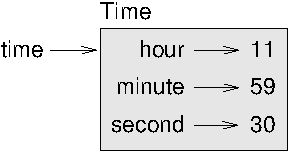
\includegraphics[scale=0.8]{figs/time.pdf}}
\caption{對象圖.}
\label{fig.time}
\end{figure}


\section{純函數}
\index{prototype and patch}
\index{development plan!prototype and patch}

下面章節中, 我們將編寫兩個函數, 實現時間計算. 
這兩個函數展示了兩種函數類型: 純函數以及修改器. 
同時, 也展示了一個我稱之為{\tt 原型和補丁}的開發範式, 
這是一種通過構建簡單原型, 逐步改進, 從而解決複雜問題的方法. 

以下為 \verb"add_time"的一個簡單原型:

\begin{verbatim}
def add_time(t1, t2):
    sum = Time()
    sum.hour = t1.hour + t2.hour
    sum.minute = t1.minute + t2.minute
    sum.second = t1.second + t2.second
    return sum
\end{verbatim}
%
該函數新建了一個{\tt Time}對象, 並初始化其屬性, 同時返回對象的引用. 
這便稱之為{\tt 純函數}, 因為它不會修改作為參數傳入的任何對象, 
同時也不會產生其他效果, 比如顯示值或提示用戶輸入, 而僅僅是返回一個值. 
\index{pure function}
\index{function type!pure}

為了測試此函數, 新建兩個Time對象:包含某電影開始時間的{\tt start}, 
比如電影{\em Monty Python and the Holy Grail},  
以及放映時長的{\tt duration}, 此處時長為1小時35分鐘. 
\index{Monty Python and the Holy Grail}

\verb"add_time" 會計算出電影結束時間. 

\begin{verbatim}
>>> start = Time()
>>> start.hour = 9
>>> start.minute = 45
>>> start.second =  0

>>> duration = Time()
>>> duration.hour = 1
>>> duration.minute = 35
>>> duration.second = 0

>>> done = add_time(start, duration)
>>> print_time(done)
10:80:00
\end{verbatim}
%
結果值{\tt 10:80:00}, 肯定不是你想要的. 
問題在於, 函數沒有處理秒數或分鐘數相加後超過60的情況. 
遇到這種情況, 我們需要將每60秒進位到分鐘, 
每60分鐘進位到小時. 
\index{carrying, addition with}

優化後的版本如下:

\begin{verbatim}
def add_time(t1, t2):
    sum = Time()
    sum.hour = t1.hour + t2.hour
    sum.minute = t1.minute + t2.minute
    sum.second = t1.second + t2.second

    if sum.second >= 60:
        sum.second -= 60
        sum.minute += 1

    if sum.minute >= 60:
        sum.minute -= 60
        sum.hour += 1

    return sum
\end{verbatim}
%
這個函數雖然正確, 但是略顯臃腫. 
稍後我們將看到一個簡短版本. 


\section{修改器}
\label{increment}
\index{modifier}
\index{function type!modifier}

有時, 對於一個函數來說,直接修改其獲取的參數對象, 更為高效. 
在此情境中, 更改對於調用者來說, 是可見的. 
這樣的函數, 被稱之為{\bf 修改器}. 
\index{increment}

函數{\tt increment}, 是對{\tt Time}對象增加特定秒數, 
這天然便適合用修改器實現. 
下面是個初稿:

\begin{verbatim}
def increment(time, seconds):
    time.second += seconds

    if time.second >= 60:
        time.second -= 60
        time.minute += 1

    if time.minute >= 60:
        time.minute -= 60
        time.hour += 1
\end{verbatim}
%
第一行執行基本操作;
其餘的則處理我們之前看到的特殊情況. 
\index{special case}

這個函數正確嗎? 如果{\tt seconds}遠大於60, 會怎樣?

這時, 只進位一次是不夠的;
我們需要重複執行, 直到{\tt time.second}小於60.
一種解決方案是用{\tt while}語句替換{\tt if}語句. 
雖然可行, 但不夠高效. 
做個練習, 編寫一個不包含任何迴圈的{\tt increment}正確版本. 

修改器所為, 純函數皆可為. 
事實上, 有些編程語言只允許使用純函數. 
有證據表明, 使用純函數比使用修改器, 開發更快, 出錯更少. 
但有時修改器用來更方便, 而函數式程式則效率不高. 

通常, 我建議在合理的情況下, 都使用純函數, 只有在優勢明顯時才
採用修改器. 這種方法便稱之為{\bf 函數式編程模式}. 
\index{functional programming style}

做個練習, 編寫一個``純''版本的{\tt increment}函數, 使其創建並返回新的Time對象, 
而不是修改其參數. 


\section{原型與規劃}
\label{prototype}
\index{prototype and patch}
\index{development plan!prototype and patch}
\index{planned development}
\index{development plan!designed}

剛剛展示的開發方案是``原型和補丁''.
就是針對每個函數, 編寫一個可以完成基本運算的原型, 然後對其測試, 
並逐步修正錯誤. 

這種方法很有效, 尤其在你尚未對問題有深入了解時. 
但是增量修正往往會產生大量過於複雜代碼---因為需要關注特殊情況---和不可靠的代碼
---因為你很難確定是否找到了所有異常. 

另一種方法是採用{\bf 設計開發}, 用這種方法, 就是採用上帝視角處理問題, 
從而開發會容易很多. 
在這裡, 這個視角就是Time對象, 實際是三個六十進制的數字(參考\url{http://en.wikipedia.org/wiki/Sexagesimal}). 
{\tt second}屬性是``個位'', {\tt minute}屬性是``60位'', {\tt hour}屬性是``3600位''.
\index{sexagesimal}

當我們編寫\verb"add_time" 和{\tt increment}函數時, 
實際是進行60位的加法, 著就是為何我們需要從當前位進位到下一位的原因. 
\index{carrying, addition with}

這個發現給出了另一種解決問題的方法---我們將Time對象轉為整數, 
然後利用計算機善於進行整數運算的優勢. 

這是個將Time對象轉為整數的函數:

\begin{verbatim}
def time_to_int(time):
    minutes = time.hour * 60 + time.minute
    seconds = minutes * 60 + time.second
    return seconds
\end{verbatim}
%
下面函數可以將整數轉換為Time(回憶一下{\tt divmod}, 也就是將第一個參數除以第二個參數, 
將商和餘數作為元組返回). 
\index{divmod}

\begin{verbatim}
def int_to_time(seconds):
    time = Time()
    minutes, time.second = divmod(seconds, 60)
    time.hour, time.minute = divmod(minutes, 60)
    return time
\end{verbatim}
%
你可能需要費點腦力, 並運行一些測試, 以說服自己這些函數是正確的. 
一種方法是針對各種{\tt x}值, 檢查\verb"time_to_int(int_to_time(x)) == x"是否正確. 
這就是一種一致性檢驗. 
\index{consistency check}

一旦你確信它們正確, 便可以用其重寫\verb"add_time":

\begin{verbatim}
def add_time(t1, t2):
    seconds = time_to_int(t1) + time_to_int(t2)
    return int_to_time(seconds)
\end{verbatim}
%
這個版本相比原來的版本, 更容易驗證. 
試一下, 用\verb"time_to_int" 和
\verb"int_to_time"來重寫{\tt increment} . 

在某些方面, 60進制與10進制的相互轉換相比時間處理要更難. 
因為進制轉換更加抽象;
而時間處理更符合我們的直觀感受. 

但如果我們注意到時間不過是60進制的數字, 並預先編寫轉換函數 (\verb"time_to_int"
和 \verb"int_to_time"), 便可以得到一個更精簡, 易讀, 易調試, 也更可靠的程式. 

同時這也更利於後續添加新的功能. 
比如, 假如要對兩個Time對象相減, 獲取其時間間隔. 
直接的方法, 便是通過借位實現. 
但是, 使用轉換函數, 會更容易, 也更可能正確. 
\index{subtraction with borrowing}
\index{borrowing, subtraction with}
\index{generalization}

諷刺的是, 有時候將問題想得複雜(或更通用), 反而會更容易解決(因為特殊情況會更少, 
出錯概率也會更低).


\section{調試}
\index{debugging}

如果{\tt minute}和{\tt second}在0到60之間(包括0但不包括60),
同時{\tt hour}是正數, 那這個Time對象便是正確的. 
{\tt hour}和{\tt minute}應該是整數, 但{\tt second}可以允許有小數部分. 
\index{invariant}

這種約束條件, 叫做{\bf 不變式}, 因為它們需要恆為真. 
換句話說, 如果它們不是真, 那肯定有某些地方出錯了. 

編寫代碼來檢查不變式, 可以幫助發現錯誤並找出原因. 
比如, 你可能有個函數\verb"valid_time" , 它會接收一個Time對象, 
如果違反了不變式的某個條件, 返回{\tt False}:

\begin{verbatim}
def valid_time(time):
    if time.hour < 0 or time.minute < 0 or time.second < 0:
        return False
    if time.minute >= 60 or time.second >= 60:
        return False
    return True
\end{verbatim}
%
在每個函數的開始部分, 你都可以檢查參數並確保它們合法:
\index{raise statement}
\index{statement!raise}

\begin{verbatim}
def add_time(t1, t2):
    if not valid_time(t1) or not valid_time(t2):
        raise ValueError('invalid Time object in add_time')
    seconds = time_to_int(t1) + time_to_int(t2)
    return int_to_time(seconds)
\end{verbatim}
%
或者你也可以用{\bf assert 語句}, 檢查一個給定的不變式, 如果失敗, 拋出異常:
\index{assert statement}
\index{statement!assert}

\begin{verbatim}
def add_time(t1, t2):
    assert valid_time(t1) and valid_time(t2)
    seconds = time_to_int(t1) + time_to_int(t2)
    return int_to_time(seconds)
\end{verbatim}
%
{\tt assert}語句非常有用, 因為它們區分了何為常規條件代碼, 何為檢驗錯誤的代碼. 


\section{術語表}

\begin{description}

\item[原型和補丁(prototype and patch):] 一種通過先寫程式初稿, 然後測試, 並修正發現的錯誤的開發方案. 
\index{prototype and patch}

\item[設計開發(designed development):] 一種開發方案, 採用上帝視角處理問題, 
相比於增量開發或者原型開發, 需要更多提前規劃. 
\index{designed development}

\item[純函數(pure function):] 一種不修改任何作為參數傳入的對象的函數. 
多數純函數有返回值. 
\index{pure function}

\item[修改器(modifier):] 一種函數, 
會修改作為參數接收的一個或者多個對象. 
多數修改器都是沒有返回值的;
也就是說, 它們返回{\tt None}. \index{modifier}

\item[函數式編程風格(functional programming style):] 一種程式設計風格, 其中多數函數
都是純函數.
\index{functional programming style}

\item[不變式(invariant):] 程式執行期間, 應該始終為真的條件. 
\index{invariant}

\item[斷言語句(assert statement):] 檢查條件是否滿足, 並在失敗時拋出異常的語句. 
\index{assert statement}
\index{statement!assert}

\end{description}


\section{習題集}

本章代碼樣例在
\url{http://thinkpython2.com/code/Time1.py}; 
同時習題答案在\url{http://thinkpython2.com/code/Time1_soln.py}.

\begin{exercise}

編寫\verb"mul_time" 函數, 接收一個Time對象以及一個數字, 
返回一個原始時間和數字的乘積的新時間對象. 

然後用\verb"mul_time" 來編寫一個函數, 接收一個表示比賽結束時間的Time對象, 
以及一個表示距離的數字, 返回一個表示平均配速(每英里耗時)的Time對象. 
\index{running pace}

\end{exercise}


\begin{exercise}
\index{datetime module}
\index{module!datetime}

{\tt datetime}模塊提供的{\tt time}對象和本章的Time對象相似, 
但是前者提供了更豐富的方法和操作. 
可在\url{http://docs.python.org/3/library/datetime.html}閱讀相關文檔.

\begin{enumerate}

\item 使用 {\tt datetime} 模塊編寫程式, 獲取當前日期並打印星期幾. 

\item 編寫個程式, 輸入生日, 輸出用戶的年齡以及距離下個生日的
天數, 小時數, 分鐘數和秒數. 
\index{birthday}

\item 對於兩個生日不同的人, 
總有一天, 一個人的出生天數是另一個人的兩倍. 
我們稱之為``雙倍日''.
編寫個程式, 輸入兩個生日, 計算他們的``雙倍日''.

\item 進階一下, 編寫個更通用的版本, 計算某人的出生天數是另一個$n$倍大的那一天. 
\index{Double Day}

\end{enumerate}

參看: \url{http://thinkpython2.com/code/double.py}

\end{exercise}


\chapter{類和方法}

雖然我們已經接觸了一些Python的面向對象的特性, 
但前面兩章的內容並不算是真正的面向對象, 
因為自定義類型與操作它們的函數之間的關係, 並未涉及. 
下面會將這些函數轉換為方法, 從而使其關係明晰. 

本章代碼可以從
\url{http://thinkpython2.com/code/Time2.py}下載, 
同時習題答案在\url{http://thinkpython2.com/code/Point2_soln.py}中.


\section{面向對象特性}
\index{object-oriented programming}

Python是個{\bf 面向對象編程語言}, 
也就是說, 它提供了支持面向對象編程的諸多特性, 而面向對象編程有以下特徵:

\begin{itemize}

\item 程式包括類和方法定義.

\item 多數運算都基於對象操作而存在. 

\item 對象通常表示現實世界中的事物, 方法通常對應現實世界中事物的交互方式. 

\end{itemize}

比如, 在第~\ref{time}節定義的{\tt Time}類, 對應人們記錄一天中時間的方式, 
而我們定義的函數, 則對應了人們處理時間的不同策略. 
類似的, 第~\ref{clobjects}節的{\tt Point}和{\tt Rectangle}類, 
分別表示點和矩形的數學概念. 

到目前為止, 我們都還沒有充分使用Python提供的支持面向對象編程的強大功能. 
這些功能嚴格來說並非必須;
多數功能的語法我們都已經變相實現過了. 
但很多時候, 面向對象的語法更加簡潔, 同時更加精確地表達程式結構. 

比如, 在{\tt Time1.py}中, 類定義和函數定義並無明顯關聯. 
認真觀察, 便會發現每個函數都至少有一個{\tt Time}對象作為參數. 
\index{method}
\index{function}

透過觀察, 很自然地引出了{\bf 方法};
一個方法便是一個與某個類相關聯的函數. 
我們已經接觸過字符串, 串列, 字典和元組的方法. 
本章中, 我們將構建自定義類型的方法. 
\index{syntax}
\index{semantics}
\index{programmer-defined type}
\index{type!programmer-defined}

方法和函數, 語義相同, 但語法有兩處差異:

\begin{itemize}

\item 方法定義在類中, 以使類和方法的關係一目了然. 

\item 調用方法的語法和調用函數的語法不同. 

\end{itemize}

後面章節中, 我們將把前兩章涉及的函數轉換為方法. 
這種轉換純粹是機械性的; 通過一系列步驟便可實現. 
如果你可以熟練地從一種形式轉換為另一種形式, 
那麼你便能夠為眼下的事情, 選擇最合適的形式. 

\section{打印對象}
\index{object!printing}

在第~\ref{time}節, 我們定義了{\tt Time}類, 在第~\ref{isafter}節, 
你編寫了\verb"print_time"函數:

\begin{verbatim}
class Time:
    """Represents the time of day."""

def print_time(time):
    print('%.2d:%.2d:%.2d' % (time.hour, time.minute, time.second))
\end{verbatim}
%
若要調用函數, 需要傳遞一個{\tt Time}對象作為參數:

\begin{verbatim}
>>> start = Time()
>>> start.hour = 9
>>> start.minute = 45
>>> start.second = 00
>>> print_time(start)
09:45:00
\end{verbatim}
%

要使\verb"print_time" 成為方法, 只需要將函數定義移動到類定義內部. 
同時注意縮進的變化. 
\index{indentation}

\begin{verbatim}
class Time:
    def print_time(time):
        print('%.2d:%.2d:%.2d' % (time.hour, time.minute, time.second))
\end{verbatim}
%
現在有兩種方式調用\verb"print_time" . 
第一種(也是不常用的)方式是使用函數語法:
\index{function syntax}
\index{dot notation}

\begin{verbatim}
>>> Time.print_time(start)
09:45:00
\end{verbatim}
%
這裡用到了點標法, {\tt Time}是類的名稱, 
\verb"print_time"是方法的名稱. 
{\tt start}是傳入的參數. 

第二種(也是更簡潔的)方式, 是使用方法語法:
\index{method syntax}

\begin{verbatim}
>>> start.print_time()
09:45:00
\end{verbatim}
%
這裡也用了點標法, \verb"print_time" 也是方法的名字, {\tt start}是調用方法的對象, 
也被稱為{\tt 主體}. 
正如句子的主語是句子主體, 方法的調用主體也就是方法的主體. 
\index{subject}

在方法內部, 主體被賦值給了第一個參數, 所以在這裡{\tt start}被賦值給了{\tt time}.
\index{self (parameter name)}
\index{parameter!self}

按照慣例, 方法的第一個參數稱為{\tt self}, 所以\verb"print_time"的常見寫法如下:

\begin{verbatim}
class Time:
    def print_time(self):
        print('%.2d:%.2d:%.2d' % (self.hour, self.minute, self.second))
\end{verbatim}
%

這種約定是有其內在緣由的:
\index{metaphor, method invocation}

\begin{itemize}

\item 函數調用的語法, \verb"print_time(start)",  表示函數是主動一方. 
就像, ``嘿, \verb"print_time"!  這有個對象需要你打印一下.''

\item 在面向對象編程中, 對象是主動一方. 像\verb"start.print_time()"這種方法調用, 
就像是說, ``嗨, {\tt start}! 請打印你自己. ''

\end{itemize}

這種視角的轉換看似更優雅了, 但並沒有明顯的優勢. 
在目前遇到的例子中, 看不出什麼差異. 
但有時候, 將觸發者從函數轉移到對象上, 
可以寫出更通用的函數(或方法), 便於後期維護和復用. 

做個練習, 將\verb"time_to_int"(見第~\ref{prototype}節), 重寫為方法. 
你可以嘗試將\verb"int_to_time" 也重寫為方法, 但沒有什麼意義, 
因為沒有對象可以調用它. 


\section{另一個示例}
\index{increment}

下面是 {\tt increment}(章節~\ref{increment})作為方法的重寫版本:

\begin{verbatim}
# inside class Time:

    def increment(self, seconds):
        seconds += self.time_to_int()
        return int_to_time(seconds)
\end{verbatim}
%
這個版本假設 \verb"time_to_int" 已經被重寫為了方法. 
同時, 也要注意它是一個純函數, 而不是修改器. 

下面是調用{\tt increment}的方式:

\begin{verbatim}
>>> start.print_time()
09:45:00
>>> end = start.increment(1337)
>>> end.print_time()
10:07:17
\end{verbatim}
%
主體{\tt start}, 被賦值給了第一個參數{\tt self}. 
實參{\tt 1337}, 則被分配給了第二個參數, {\tt seconds}. 

這種機制讓人感覺很迷惑, 尤其是產生錯誤的時候. 
比如, 如果你用兩個實參調用{\tt increment}, 會報錯:
\index{exception!TypeError}
\index{TypeError}

\begin{verbatim}
>>> end = start.increment(1337, 460)
TypeError: increment() takes 2 positional arguments but 3 were given
\end{verbatim}
%
這個錯誤信息初看很難理解, 因為括號裡只有兩個參數. 
但這個主體也被當作了一個參數, 所以一共有三個. 

另外, {\bf 位置參數}是沒有參數名的參數;
也就是說, 它不是關鍵字參數. 
下面函數調用中:
\index{positional argument}
\index{argument!positional}

\begin{verbatim}
sketch(parrot, cage, dead=True)
\end{verbatim}

{\tt parrot}和{\tt cage}是位置參數, 而{\tt dead}是
關鍵字參數.


\section{一個進階案例}

重寫\verb"is_after"(見第~\ref{isafter}節)會略微複雜, 因為它需要兩個Time對象作為參數. 
這種情況, 通常將第一個參數命名為{\tt self}, 第二個命名為{\tt other}:
\index{other (parameter name)}
\index{parameter!other}

\begin{verbatim}
# inside class Time:

    def is_after(self, other):
        return self.time_to_int() > other.time_to_int()
\end{verbatim}
%
若要使用此方法, 你需要在某個對象上調用此方法, 並將另一個對象作為參數傳入:

\begin{verbatim}
>>> end.is_after(start)
True
\end{verbatim}
%
這種語法的一個好處, 是它讀起來如同英語: ``end is after start?''


\section{init方法}
\index{init method}
\index{method!init}

init方法(``initialization''的簡稱)是一個特殊的方法, 
在對象被實例化時才被調用. 
其全稱為\verb"__init__"(兩個下劃線, 然後緊跟{\tt init}, 然後又是兩個下劃線).
{\tt Time}類的init方法如下:

\begin{verbatim}
# inside class Time:

    def __init__(self, hour=0, minute=0, second=0):
        self.hour = hour
        self.minute = minute
        self.second = second
\end{verbatim}
%
通常\verb"__init__"方法的參數名稱和類中屬性名稱相同. 
下面語句

\begin{verbatim}
        self.hour = hour
\end{verbatim}
%
會將參數{\tt hour}的值存儲為{\tt self}的一個屬性.
\index{optional parameter}
\index{parameter!optional}
\index{default value}
\index{override}

這個參數是可選的, 所以如果你調用{\tt Time}時沒有傳參, 
那便會使用默認值. 

\begin{verbatim}
>>> time = Time()
>>> time.print_time()
00:00:00
\end{verbatim}
%
如果你提供了一個參數, 那只會覆蓋{\tt hour}:

\begin{verbatim}
>>> time = Time (9)
>>> time.print_time()
09:00:00
\end{verbatim}
%
如果提供了兩個參數, 則會覆寫{\tt hour}和{\tt minute}.

\begin{verbatim}
>>> time = Time(9, 45)
>>> time.print_time()
09:45:00
\end{verbatim}
%
如果提供三個參數, 則會覆寫三個默認值. 

做個練習, 為{\tt Point}類編寫init方法, 使用{\tt x}和 {\tt y} 作為可選參數, 
並賦值給相應的屬性. 
\index{Point class}
\index{class!Point}


\section{{\tt \_\_str\_\_}方法}
\index{str method@\_\_str\_\_ method}
\index{method!\_\_str\_\_}

\verb"__str__" 和 \verb"__init__"類似, 也是一個特殊的方法, 
其一般返回對象的字符串表示. 
\index{string representation}

比如, 下面是Time對象的{\tt str}方法:

\begin{verbatim}
# inside class Time:

    def __str__(self):
        return '%.2d:%.2d:%.2d' % (self.hour, self.minute, self.second)
\end{verbatim}
%
當用{\tt print}打印對象時, Python調用的就是{\tt str}方法:
\index{print statement}
\index{statement!print}

\begin{verbatim}
>>> time = Time(9, 45)
>>> print(time)
09:45:00
\end{verbatim}
%
當編寫新類時, 我總是先寫\verb"__init__"方法, 這樣更容易初始化對象, 
同時編寫\verb"__str__"方法, 以方便調試. 

試著為{\tt Point}類編寫{\tt str}方法. 
創建一個Point對象, 並打印輸出. 


\section{運算子重載}
\label{operator.overloading}

通過定義一些特殊方法, 你可以對自定義類型, 重新定義運算子的行為. 
比如, 你為{\tt Time}類定義了\verb"__add__" 方法, 便可以用{\tt +}運算子操作Time對象. 
\index{programmer-defined type}
\index{type!programmer-defined}

如下定義:
\index{add method}
\index{method!add}

\begin{verbatim}
# inside class Time:

    def __add__(self, other):
        seconds = self.time_to_int() + other.time_to_int()
        return int_to_time(seconds)
\end{verbatim}
%
可以這樣使用:

\begin{verbatim}
>>> start = Time(9, 45)
>>> duration = Time(1, 35)
>>> print(start + duration)
11:20:00
\end{verbatim}
%
當對Time對象應用{\tt +}運算子時, Python會調用\verb"__add__".
當打印結果時, Python會調用\verb"__str__".
所以我們看到的, 只是冰山一角而已!
\index{operator overloading}

對自定義類型, 改變運算子的行為, 這便是{\bf 運算子重載}. 
對於Python中的每個運算子, 都有一個類似\verb"__add__"的特殊方法與之對應. 
更多詳細信息, 請參考
\url{http://docs.python.org/3/reference/datamodel.html#specialnames}.

作為練習, 請為Point類編寫{\tt add}方法. 

\section{類型分發}

在上一節, 我們將兩個Time對象進行加法操作, 
但是你可能想將一個整數與Time對象相加. 
下面是一個\verb"__add__"的新版本, 它會檢驗{\tt other}的類型, 
從而決定調用\verb"add_time" , 還是{\tt increment}方法:

\begin{verbatim}
# inside class Time:

    def __add__(self, other):
        if isinstance(other, Time):
            return self.add_time(other)
        else:
            return self.increment(other)

    def add_time(self, other):
        seconds = self.time_to_int() + other.time_to_int()
        return int_to_time(seconds)

    def increment(self, seconds):
        seconds += self.time_to_int()
        return int_to_time(seconds)
\end{verbatim}
%
內置函數{\tt isinstance}會接收一個值和一個類對象, 
如果值是這個類的實例, 則返回{\tt True}.
\index{isinstance function}
\index{function!isinstance}

如果{\tt other} 是一個Time對象, 
\verb"__add__"會調用\verb"add_time". 
否則, 會認為參數是個數字, 從而調用{\tt increment}方法. 
這種操作叫做{\tt 類型分發}, 因為它基於參數的類型不同, 
將計算任務分發給不同的方法. 
\index{type-based dispatch}
\index{dispatch, type-based}

下面時一個在不同類型上使用{\tt +}運算子的例子:

\begin{verbatim}
>>> start = Time(9, 45)
>>> duration = Time(1, 35)
>>> print(start + duration)
11:20:00
>>> print(start + 1337)
10:07:17
\end{verbatim}
%
不幸的是, 這個加法的實現並不具有可交換性. 
如果整數在前, 你會得到報錯:
\index{commutativity}

\begin{verbatim}
>>> print(1337 + start)
TypeError: unsupported operand type(s) for +: 'int' and 'instance'
\end{verbatim}
%
問題在於, Python並不是對Time對象加上一個整數, 
而是對一個整數加上Time對象, 
所以不知道如何處理了. 
有個取巧的解決辦法: 用特殊方法\verb"__radd__", 表示``右側相加''. 
當Time對象出現在{\tt +}運算子右側時, 將調用此方法. 
以下是定義:
\index{radd method}
\index{method!radd}

\begin{verbatim}
# inside class Time:

    def __radd__(self, other):
        return self.__add__(other)
\end{verbatim}
%
下面是使用方式:

\begin{verbatim}
>>> print(1337 + start)
10:07:17
\end{verbatim}
%

做個練習, 為Points編寫{\tt add}方法, 使其同時適用於Point對象和元組:

\begin{itemize}

\item 如果第二個操作數是Point對象, 方法則返回一個新的Point, 
其$x$坐標是操作數的$x$坐標總和, $y$坐標同理. 

\item 如果第二個操作數是元組, 則方法應該將元組的第一個元素和$x$坐標相加, 
第二個元素和$y$坐標相加, 然後返回此結果的一個新Point對象. 

\end{itemize}


\section{多態性}
\label{polymorphism}

當需要的時候, 基於類型分發是有用的, 但(幸好)不用總要如此. 
通常, 你可以編寫適用不同類型參數的函數, 來避免類型分發. 
\index{type-based dispatch}
\index{dispatch!type-based}

我們為字符串操作編寫的很多函數, 對於其他序列類型也適用. 
比如, 在第~\ref{histogram}節, 我們用{\tt histogram} 來統計單詞中每個字母出現的次數. 

\begin{verbatim}
def histogram(s):
    d = dict()
    for c in s:
        if c not in d:
            d[c] = 1
        else:
            d[c] = d[c]+1
    return d
\end{verbatim}
%
這個函數對於串列, 元組, 甚至字典都適用, 只要{\tt s}中的元素是可哈希的, 
就都可以作為{\tt d}的鍵. 

\begin{verbatim}
>>> t = ['spam', 'egg', 'spam', 'spam', 'bacon', 'spam']
>>> histogram(t)
{'bacon': 1, 'egg': 1, 'spam': 4}
\end{verbatim}
%
能夠處理多種類型的函數, 稱為{\bf 多態}. 
多態性有助於代碼復用. 
例如, 可以對序列中元素求和的內置函數{\tt sum}, 
也同樣適用於其他支持加法運算的元素序列. 
\index{polymorphism}

因為Time對象也提供了{\tt add}方法, 所以也同樣適用於{\tt sum}:

\begin{verbatim}
>>> t1 = Time(7, 43)
>>> t2 = Time(7, 41)
>>> t3 = Time(7, 37)
>>> total = sum([t1, t2, t3])
>>> print(total)
23:01:00
\end{verbatim}
%
通常, 如果函數內的所有操作適用於某種類型, 那麼這個函數便同樣適用於此類型. 

最好的多態, 是那種不求而得, 
就像你突然發現你寫的函數, 對於規劃之外的某種類型, 也同樣適用. 


\section{調試}
\index{debugging}

在程式運行的任何時刻, 向對象添加屬性都是可行的, 
但如果對象類型相同, 屬性不同, 那很容易出錯. 
所以比較好的方法是在init方法中初始化對象的全部屬性. 
\index{init method}
\index{attribute!initializing}

如果你不確定一個對象是否包含某個屬性, 可以適用內置函數{\tt hasattr}
 (見第~\ref{hasattr}節)進行判斷. 
\index{hasattr function}
\index{function!hasattr}
\index{dict attribute@\_\_dict\_\_ attribute}
\index{attribute!\_\_dict\_\_}

另一種獲取屬性的方式, 是使用內置函數{\tt vars},
它會接收一個對象, 並返回一個屬性名(字符串格式)映射到屬性值的字典:

\begin{verbatim}
>>> p = Point(3, 4)
>>> vars(p)
{'y': 4, 'x': 3}
\end{verbatim}
%

對於調試而言, 你會發現保留下面的函數, 會很有用:

\begin{verbatim}
def print_attributes(obj):
    for attr in vars(obj):
        print(attr, getattr(obj, attr))
\end{verbatim}
%
\verb"print_attributes"會遍歷字典, 輸出每個屬性名稱以及其對應的值. 
\index{traversal!dictionary}
\index{dictionary!traversal}

內置函數{\tt getattr}會接收一個對象和一個屬性名(字符串格式), 返回該屬性的值. 
\index{getattr function}
\index{function!getattr}


\section{介面和實現}

面向對象設計的一個目標便是令軟體便於維護, 
也就是說當系統的某些部分發生了變化, 你依然可以保證程式正常運行, 
從而可以修改程式, 以滿足新的需求. 
\index{interface}
\index{implementation}
\index{maintainable}
\index{object-oriented design}

實現這一目標的一個設計原則便是, 介面和實現分離. 
對於對象來說, 就是類提供的方法不應該依賴於屬性的形式. 
\index{attribute}

比如, 本章我們開發了一個類, 表示一天中某個時間. 
這個類提供的方法包括
\verb"time_to_int", \verb"is_after", 以及\verb"add_time".

我們有多種方式實現這些方法. 
實現的細節取決於我們如何表示時間. 
在本章, {\tt Time}對象的屬性有{\tt hour}, {\tt minute}, 和
{\tt second}. 

同樣的, 我們也可以用一個整數, 即從零點以來的秒數來表示這些屬性. 
這種實現方式, 將會令某些方法, 比如\verb"is_after", 更容易實現, 而令某些方法更難編寫. 

當你應用了一個新的類後, 你可能發現更好的實現方式. 
但如果程式的其他部分正在使用你的類, 這時候修改介面, 
往往比較耗時, 且容易出錯. 

但如果你設計介面時足夠仔細, 你便可以在不改變介面的同時, 修改內部實現, 
也就意味著程式其他部分無需變動. 


\section{術語表}

\begin{description}

\item[面向對象語言(object-oriented language):] 提供自定義類型和方法等特性, 
以方便麵向對象編程的語言. 
\index{object-oriented language}

\item[面向對象編程(object-oriented programming):] 
一種將數據和操作
封裝進類和方法中的編程風格.
\index{object-oriented programming}

\item[方法(method):] 定義在類定義中的函數, 
在該類的實例上被調用. 
\index{method}

\item[主體(subject):] 方法調用所基於的對象. 
\index{subject}

\item[位置參數(positional argument):] 不包括參數名稱的參數, 
所以不是關鍵字參數. 
\index{positional argument}
\index{argument!positional}

\item[運算子重載(operator overloading):] 修改類似{\tt +}這樣運算子的操作, 
從而令其適用於自定義類型. 
\index{overloading}
\index{operator!overloading}

\item[類型分發(type-based dispatch):] 一種編程模式, 檢驗操作對象的類型, 
並根據不同類型, 調用不同的函數. 
\index{type-based dispatch}

\item[多態(polymorphic):] 表示函數可以應用於多種類型的特性. 
\index{polymorphism}

\end{description}


\section{習題集}

\begin{exercise}

從\url{http://thinkpython2.com/code/Time2.py}下載本章代碼. 
修改{\tt Time}的屬性為整數, 用來表示從午夜零點計時的秒數. 
然後修改方法(以及\verb"int_to_time"函數), 以適應新的實現. 
你不必修改{\tt main}中的測試代碼. 
完成修改後, 輸出應該和以前一樣. 
參考答案: \url{http://thinkpython2.com/code/Time2_soln.py}.

\end{exercise}


\begin{exercise}
\label{kangaroo}
\index{default value!avoiding mutable}
\index{mutable object, as default value}
\index{worst bug}
\index{bug!worst}
\index{Kangaroo class}
\index{class!Kangaroo}

這個習題是個警示故事, 涉及了Python中一個最常見, 卻最難發現的錯誤. 
編寫一個名為{\tt Kangaroo}的類, 需要包含下面的方法:

\begin{enumerate}

\item 一個\verb"__init__" 方法, 初始化一個名為\verb"pouch_contents"的屬性, 
使其為空串列. 

\item 一個名為\verb"put_in_pouch"的方法, 使其接收一個任意類型對象, 並將其放入
\verb"pouch_contents"中. 

\item 一個\verb"__str__" 方法, 返回一個字符串格式的 Kangaroo 對象和 \verb"pouch_contents" 中的內容. 

\end{enumerate}
%
創建兩個{\tt Kangaroo}對象, 將其分別賦值給{\tt kanga}和{\tt roo}, 
然後將{\tt roo}添加到{\tt kanga}的\verb"pouch_contents"中, 測試代碼. 

從\url{http://thinkpython2.com/code/BadKangaroo.py}下載代碼. 
代碼裡面是上面習題的一個答案, 
可是其中有個又大又棘手的錯誤. 找到並修復這個錯誤. 

如果你難以解決, 可以下載
\url{http://thinkpython2.com/code/GoodKangaroo.py}, 
在這裡面詳細解釋了問題所在, 並展示了一個解決方案. 
\index{aliasing}
\index{embedded object}
\index{object!embedded}

\end{exercise}


\chapter{繼承}

面向對象編程中涉及最多的語言特性, 便是{\bf 繼承}. 
繼承是一種基於已有類, 進行修改, 從而定義新的類的能力. 
本章我將用表示撲克牌, 一副牌以及牌型的類來講解何為繼承. 
\index{deck} 
\index{card, playing} 
\index{poker}

如果你不玩撲克, 你可以從\url{http://en.wikipedia.org/wiki/Poker}入門. 
不過也不必糾結, 因為我稍後會講解清楚練習所涉及的內容. 

本章代碼樣例在
\url{http://thinkpython2.com/code/Card.py}.


\section{紙牌對象}

一副撲克有五十二張牌, 每個都屬於四種花色中的一種, 同時也是十三個等級牌之一. 
四種花色分別為黑桃, 紅心, 方塊和梅花(橋牌中降序排列). 
等級分別是A, 2, 3, 4, 5, 6, 7, 8, 9, 10, J, Q 和K. 根據玩法不同, 
A可能比K大, 或者比2小. 
\index{rank}
\index{suit}

如果你想定義個新對象來表示一張牌, 
很明顯有兩個屬性: {\tt 等級}和{\tt 花色}.
至於屬性用何類型表示, 就不太明顯了. 
一種方式是用字符串表示, 比如\verb"'黑桃'"表示花色, 
\verb"'Q'"表示等級. 
但這種實現方式有個問題, 比較哪張牌的等級或者花色更高, 便不太容易了. 
\index{encode}
\index{encrypt}
\index{map to}
\index{representation}

另一種方式是用整數來{\bf 編碼}等級和花色. 
在這裡, ``編碼'' 表示我們定義一個數字和花色, 或者數字和等級之間的映射. 
這種編碼並不是為了保密(而是``加密''). 

\newcommand{\mymapsto}{$\mapsto$}

舉例來說, 下面表格展示了花色和相應整數編碼:

\begin{tabular}{l c l}
黑桃(Spades) & \mymapsto & 3 \\
紅心(Hearts) & \mymapsto & 2 \\
方塊(Diamonds) & \mymapsto & 1 \\
梅花(Clubs) & \mymapsto & 0
\end{tabular}

通過編碼, 比較牌的大小便容易很多;
因為更高的花色對應了更高的數字, 我們可以通過比較它們的編碼來比較花色大小. 

等級的映射編碼更容易明白了; 
每個數字等級對應相應的整數, 對於臉牌, 編碼如下:

\begin{tabular}{l c l}
J(Jack) & \mymapsto & 11 \\
Q(Queen) & \mymapsto & 12 \\
K(King) & \mymapsto & 13 \\
\end{tabular}

我用\mymapsto~符號表示映射比較清晰明了, 但不能寫入Python程式中. 
它們只是程式設計的一部分, 不應出現在代碼中. 
\index{Card class}
\index{class!Card}

{\tt Card} 的類定義如下:

\begin{verbatim}
class Card:
    """Represents a standard playing card."""

    def __init__(self, suit=0, rank=2):
        self.suit = suit
        self.rank = rank
\end{verbatim}
%
通常, init方法對每個屬性都接收一個可選參數. 
默認的卡牌是梅花2.
\index{init method}
\index{method!init}

使用你想要的花色和等級, 調用{\tt Card}類, 便可以創建一個新的Card對象. 

\begin{verbatim}
queen_of_diamonds = Card(1, 12)
\end{verbatim}
%


\section{類屬性}
\label{class.attribute}
\index{class attribute}
\index{attribute!class}

若要以人們容易理解的方式打印Card對象, 我們需要
將整數編碼映射到相應等級和花色. 
很自然想到使用字符串串列來實現. 
我們將串列賦值給{\bf 類屬性}:

\begin{verbatim}
# inside class Card:

    suit_names = ['Clubs', 'Diamonds', 'Hearts', 'Spades']
    rank_names = [None, 'Ace', '2', '3', '4', '5', '6', '7', 
              '8', '9', '10', 'Jack', 'Queen', 'King']

    def __str__(self):
        return '%s of %s' % (Card.rank_names[self.rank],
                             Card.suit_names[self.suit])
\end{verbatim}
%
像變量\verb"suit_names" 和\verb"rank_names"一樣, 
定義在類的內部, 但同時在方法外部的變量, 叫做類屬性, 
因為它們屬於{\tt Card}這個類對象. 
\index{instance attribute}
\index{attribute!instance}

這將其與類似{\tt suit}和{\tt rank}的{\bf 實例屬性}進行了區分, 
因為實例屬性和特定實例相關聯. 
\index{dot notation}

無論何種類型的屬性, 都是通過點標法來獲取. 
比如, 在\verb"__str__"中, {\tt self}是指卡牌對象, 
同時{\tt self.rank}是其等級. 同樣, {\tt Card}是個類對象, 
\verb"Card.rank_names"表示與類相關的字符串串列. 

每個卡牌都有自己的{\tt suit}和{\tt rank}, 
但\verb"suit_names" 和 \verb"rank_names"只有一份副本. 

綜合來看, 表達式\verb"Card.rank_names[self.rank]" 
表示``用{\tt self}對象的{\tt rank}屬性作為索引, 
從{\tt Card}類的\verb"rank_names"串列中, 獲取相應的字符串.''

\verb"rank_names"的第一個元素是{\tt None},
因為沒有卡牌的等級為零. 
通過囊括{\tt None}作為一個占位符, 
從而令索引2恰到好處地映射到了字符串\verb"'2'", 其他一樣. 
如果不想要這種取巧操作, 可以用字典替代串列. 

利用現有方法, 我們可以創建並打印紙牌:

\begin{verbatim}
>>> card1 = Card(2, 11)
>>> print(card1)
Jack of Hearts
\end{verbatim}

\begin{figure}
\centerline
{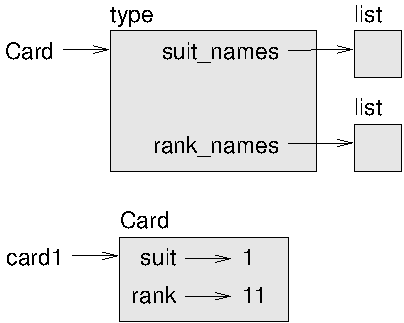
\includegraphics[scale=0.8]{figs/card1.pdf}}
\caption{對象圖.}
\label{fig.card1}
\end{figure}

圖~\ref{fig.card1}是{\tt Card}類對象和一個Card實例的對象圖;
{\tt Card}是個類對象, 其類型是{\tt type}.  
{\tt card1}是{\tt Card}的一個實例, 
所以其類型是{\tt Card}.
為了節約空間, 我沒有畫出\verb"suit_names"和\verb"rank_names"的內容. 
\index{state diagram}
\index{diagram!state} \index{object diagram} \index{diagram!object}


\section{比較卡牌}
\label{comparecard}
\index{operator!relational}
\index{relational operator}

對於內置類型, 有比較運算子({\tt <}, {\tt >}, {\tt ==}, 等.)
可以比較值, 並判斷一個值大於, 小於或者等於另一個. 
對於自定義類型, 我們可以提供一個表示``小於''的\verb"__lt__"方法, 
來覆蓋內置運算子的操作. 
\index{programmer-defined type}
\index{type!programmer-defined}

\verb"__lt__" 接收兩個參數, {\tt self}和{\tt other},
並在{\tt self}小於{\tt other}時返回{\tt True}.
\index{override}
\index{operator overloading}

然而卡牌的正確順序並不明瞭. 
比如, 梅花3和方塊2, 哪個更好?
一個等級高, 一個花色大. 
若要比較兩個牌大小, 你首先需要確定等級和花色, 哪個更重要. 

答案取決於玩的何種遊戲,
但簡便起見, 我們定義花色更重要, 所以所有的黑桃大於任意方塊, 以此類推. 
\index{cmp method@\_\_cmp\_\_ method}
\index{method!\_\_cmp\_\_}

定好規則, 我們便可以編寫\verb"__lt__"了:

\begin{verbatim}
# inside class Card:

    def __lt__(self, other):
        # check the suits
        if self.suit < other.suit: return True
        if self.suit > other.suit: return False

        # suits are the same... check ranks
        return self.rank < other.rank
\end{verbatim}
%
使用元組來比較, 更加簡潔:
\index{tuple!comparison}
\index{comparison!tuple}

\begin{verbatim}
# inside class Card:

    def __lt__(self, other):
        t1 = self.suit, self.rank
        t2 = other.suit, other.rank
        return t1 < t2
\end{verbatim}
%
做個練習, 為Time對象編寫\verb"__lt__"方法. 
你可以用元組進行比較, 也可以考慮比較整數. 


\section{整副牌}
\index{list!of objects}
\index{deck, playing cards}

現在我們有Card類了, 下一步要定義整副牌(Deck)了. 
既然整副牌是由卡牌構成, 那自然每副牌都應該包含一個卡牌串列作為屬性. 
\index{init method}
\index{method!init}

下面是{\tt Deck}的類定義. 
init方法新建了一個{\tt cards}屬性, 
同時生成了標準的52張牌:
\index{composition}
\index{loop!nested}
\index{Deck class}
\index{class!Deck}

\begin{verbatim}
class Deck:

    def __init__(self):
        self.cards = []
        for suit in range(4):
            for rank in range(1, 14):
                card = Card(suit, rank)
                self.cards.append(card)
\end{verbatim}
%
生成一副牌最容易的方法便是嵌套迴圈了. 
外層迴圈枚舉了0到3的花色. 
內層迴圈枚舉了1至13的等級. 
每次疊代都會用當前花色和等級創建一張牌, 
並將其附加到{\tt self.cards}中. 
\index{append method}
\index{method!append}


\section{打印整副牌}
\label{printdeck}
\index{str method@\_\_str\_\_ method}
\index{method!\_\_str\_\_}

下面是{\tt Deck}的\verb"__str__"方法:

\begin{verbatim}
# inside class Deck:

    def __str__(self):
        res = []
        for card in self.cards:
            res.append(str(card))
        return '\n'.join(res)
\end{verbatim}
%
這個方法展示了一個拼接超大字符串的高效方法: 建立一個字符串串列, 然後使用字符串方法{\tt join}進行拼接. 
內置函數{\tt str}會對每個card都應用\verb"__str__"方法, 以返回字符串格式.
\index{accumulator!string} \index{string!accumulator}
\index{join method} \index{method!join} \index{newline}

我們在換行符上調用了{\tt join}方法, 卡牌之間被分隔成了新行. 
下面是結果示例:

\begin{verbatim}
>>> deck = Deck()
>>> print(deck)
Ace of Clubs
2 of Clubs
3 of Clubs
...
10 of Spades
Jack of Spades
Queen of Spades
King of Spades
\end{verbatim}
%
雖然結果看起來是52行, 但它其實是一個包含換行符的長字符串. 


\section{添加, 移除, 洗牌和排序}

若要發牌, 首先需要一個能夠從整副牌中移除並返回此對象的方法. 
串列方法{\tt pop}提供了一種便捷的方法:
\index{pop method}
\index{method!pop}

\begin{verbatim}
# inside class Deck:

    def pop_card(self):
        return self.cards.pop()
\end{verbatim}
%
由於{\tt pop}是從串列中移除{\em 最後一張}牌, 所以我們從底部發牌. 
\index{append method}
\index{method!append}

若要添加一張牌, 可以用串列方法{\tt append}:

\begin{verbatim}
# inside class Deck:

    def add_card(self, card):
        self.cards.append(card)
\end{verbatim}
%
像上面這樣僅使用另一個方法, 而不做過多操作, 有時被稱為{\bf veneer(裝飾)}. 
這個比喻來自於木工行業, 在一塊便宜木頭表面貼一層優質的薄木板, 進行偽裝, 
從而改善外觀. 
\index{veneer}

這裡, \verb"add_card" 是一個``薄''方法, 用卡牌術語的方式, 表達串列操作. 
而這會令實現的外觀, 或者介面, 容易理解. 

再舉個例子, 我們可以用{\tt random}模塊中的{\tt shuffle}函數, 為Deck編寫一個
{\tt shuffle}方法:
\index{random module}
\index{module!random}
\index{shuffle function}
\index{function!shuffle}

\begin{verbatim}
# inside class Deck:
            
    def shuffle(self):
        random.shuffle(self.cards)
\end{verbatim}
%
不要忘記引入{\tt random}模塊.

做個練習, 用串列方法{\tt sort}為Deck編寫一個{\tt sort}方法, 
為{\tt Deck}中的卡牌排序. 
{\tt sort}方法會使用我們定義的\verb"__lt__"方法來確定順序. 
\index{sort method} \index{method!sort}



\section{繼承}
\index{inheritance}
\index{object-oriented programming}

繼承是一種基於已有類進行修改, 從而定義新類的能力. 
比如, 我們想要一個類來表示``手牌'', 即玩家手中持有的牌. 
一副手牌和整副牌相差無幾:都是由卡牌構成, 並且都需要支持添加和移除牌等操作. 

但二者也有差異:有些手牌需要某些操作, 但整副牌卻不需要. 比如, 在
撲克牌中, 我們可能需要比較兩幅手牌, 看哪個獲勝. 
在橋牌中, 我們可能需要計算手牌的分數, 以便下注. 

類之間這種---相似卻又不同---的關係, 非常適合使用繼承. 
若要定義一個繼承自現有類的新類, 只需要將現有類的名稱放在括號中即可:
\index{parentheses!parent class in}
\index{parent class}
\index{class!parent}
\index{Hand class}
\index{class!Hand}

\begin{verbatim}
class Hand(Deck):
    """Represents a hand of playing cards."""
\end{verbatim}
%
這個定義表明{\tt Hand}繼承自{\tt Deck};
也就是說, 我們可以像Deck一樣對Hand應用\verb"pop_card"和\verb"add_card"方法.

當一個新類繼承自現有類, 那麼現有的類叫做{\bf 父類}, 
新的類叫做{\bf 子類}.
\index{parent class}
\index{child class}
\index{class!child}

在本例中, {\tt Hand}從{\tt Deck}繼承了\verb"__init__"方法, 
但沒有滿足我們的需求:init方法本應用空串列初始化{\tt cards}, 
而不是用52張新牌. 
\index{override} \index{init method}
\index{method!init}

如果我們在{\tt Hand}類中提供了init方法, 那它會覆寫{\tt Deck}類中的init方法:

\begin{verbatim}
# inside class Hand:

    def __init__(self, label=''):
        self.cards = []
        self.label = label
\end{verbatim}
%
當你創建一個Hand時, Python便會調用這個init方法, 而不是{\tt Deck}中的那個. 

\begin{verbatim}
>>> hand = Hand('new hand')
>>> hand.cards
[]
>>> hand.label
'new hand'
\end{verbatim}
%
其他的方法從{\tt Deck}繼承而來, 所以我們可以用
\verb"pop_card"和\verb"add_card"方法來發牌:

\begin{verbatim}
>>> deck = Deck()
>>> card = deck.pop_card()
>>> hand.add_card(card)
>>> print(hand)
King of Spades
\end{verbatim}
%
很顯然, 下一步就是要把這些代碼封裝進一個叫\verb"move_cards"的方法中:
\index{encapsulation}

\begin{verbatim}
# inside class Deck:

    def move_cards(self, hand, num):
        for i in range(num):
            hand.add_card(self.pop_card())
\end{verbatim}
%

\verb"move_cards"方法接受兩個參數, 一個Hand對象, 一個發牌數量. 
同時它也會修改{\tt self}和{\tt hand}, 並返回{\tt None}.

在某些遊戲中, 卡牌會從一副手牌, 移到另一副手牌, 或者
從手牌退還到牌堆中. 
你可以使用\verb"move_cards"來執行這些操作: {\tt self}可以是
一個Deck, 或者一副Hand, 儘管名字叫Hand, 但也可以是一個{\tt Deck}.

繼承是種很有用的特性. 
某些沒用繼承的重複性代碼, 使用繼承可以變得更優雅. 
繼承也方便了代碼復用, 你可以通過修改父類行為, 
為子類都添加行為. 
在某些情況下, 繼承的結構反映了問題的真正結構, 也就使得
設計更易於理解. 

另一方面, 繼承會使程式變得難以閱讀. 
當調用一個方法時, 有時很難搞明白它的定義在哪裡. 
相關代碼可能分散在數個模塊. 
此外, 許多使用繼承實現的事情, 不用繼承也能做到, 甚至做得更好. 


\section{類圖}
\label{class.diagram}

我們已經接觸過表示程式狀態的堆疊圖, 以及展示對象的屬性以及值的對象圖. 
這些圖好比程式運行時的快照, 因此也會隨著程式運行而變化. 

它們通常很詳細; 但對於某些目的來說, 偏於細緻. 
類圖是程式結構的一種更抽象的表達. 
它不展示單獨對象, 而是表示類和類之間的關係. 

類之間有多種關係:

\begin{itemize}

\item 一個類中的對象可以包括其他類中對象的引用. 
例如, 每個Rectangle都包含了一個對Point的引用,
同時每個Deck包含了多個Card的引用. 
這種關係叫做{\bf 組合(HAS-A)}, 也就是, ``一個Rectangle有一個Point.''

\item 一個類可以繼承自其他類. 
這種關係叫做{\bf 繼承(IS-A)}, 就如, ``一個Hand是一種Deck.''

\item 一個類可能依賴於另一個類, 因為類中對象可能會將其他類中的對象作為參數
使用, 或者將其他類中的對象作為計算的一部分. 
這種關係, 叫做{\bf 依賴(dependency)}.

\end{itemize}
\index{IS-A relationship}
\index{HAS-A relationship}
\index{class diagram}
\index{diagram!class}

{\bf 類圖}是這些關係的圖形化表示. 比如, 圖~\ref{fig.class1} 
展示了{\tt Card}, {\tt Deck}和{\tt Hand}之間的關係. 

\begin{figure}
\centerline
{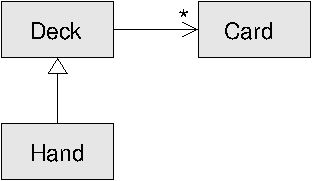
\includegraphics[scale=0.8]{figs/class1.pdf}}
\caption{類圖.}
\label{fig.class1}
\end{figure}

空心三角箭頭表示 IS-A 關係;
這裡表示Hand繼承自Deck. 

標準箭頭表示HAS-A關係;
這裡表示Deck包含Card對象的引用. 
\index{multiplicity (in class diagram)}

箭頭附近的星號({\tt *})是一個{\bf 複數表達};
表示Deck包含多少個Card. 
複數表達可以是一個{\tt 52}一樣的簡單數字, 
可以是{\tt 5..7}一樣的一個範圍, 
或者一個星號, 表示Deck可以有任意個Card. 

此類圖中沒有依賴關係. 
依賴關係通常用虛線箭頭表示. 
或者, 若有很多依賴關係存在, 它們有時候會被省略. 

一個更詳細的類圖, 可能會顯示Deck實際上包含了一個Card{\em 串列}, 
但是一般類圖中不包含串列和字典這些內置類型. 

\section{調試}
\index{debugging}

繼承可能會令調試變得困難, 因為當你調用對象的方法時, 
可能很難確定是調用的哪個方法. 
\index{inheritance}

假設你正在寫一個處理Hand對象的函數. 
你希望適用於各種牌型, 比如PokerHands, BridgeHands, 等等. 
如果你調用像{\tt Shuffle}這樣的方法, 
你可能用的是{\tt Deck}中定義的方法, 
但如果子類重寫了這個方法, 
你調用的便是子類中的方法了. 
這個特性說來是好事, 但有時令人困惑. 

如果你不確定程式執行流程的時候, 最簡單的方法便是在相關方法
開始處添加打印語句, 輸出信息. 
如果{\tt Deck.shuffle}打印了一條信息, 如{\tt Running Deck.shuffle}, 
那便可以據此來追蹤執行流程. 
\index{flow of execution}

另一個思路, 你可以用下面的函數, 接收對象和方法名稱(字符串表示), 
然後返回提供該方法定義的類:

\begin{verbatim}
def find_defining_class(obj, meth_name):
    for ty in type(obj).mro():
        if meth_name in ty.__dict__:
            return ty
\end{verbatim}
%
下面是個示例:

\begin{verbatim}
>>> hand = Hand()
>>> find_defining_class(hand, 'shuffle')
<class '__main__.Deck'>
\end{verbatim}
%
這樣便可以知道Hand中的{\tt shuffle}方法來自於{\tt Deck}.
\index{mro method}
\index{method!mro}
\index{method resolution order}

\verb"find_defining_class"函數使用{\tt mro}方法, 獲取類對象的串列, 
進而根據方法進行搜索. 
``MRO''是``method resolution order''的簡稱, 
是指Python``解析''方法名時所搜索的序列.

下面是個設計建議:當你覆蓋一個方法時, 
新方法的介面, 要和舊的保持一致. 
它應該接收同樣的參數, 返回相同的類型, 
同時遵守相同的先決條件和後置條件. 
如果你遵循上述規則, 你會發現為父類實例, 如Deck, 所設計的函數, 
也同樣適用於子類實例, 比如Hand和PokerHand. 

\index{override}
\index{interface}
\index{precondition}
\index{postcondition}

如果你違反了這個``里氏替換原理''原則, 
那代碼將很不幸地像紙牌屋一樣崩塌. 
\index{Liskov substitution principle}


\section{數據封裝}

前面章節講述了一種``面向對象設計''的開發模式. 
我們識別了對象--比如{\tt Point}, {\tt Rectangle}和{\tt Time}---同時
定義類來表示這些對象. 
在每個例子中, 對象和現實世界(或者至少是數學世界)實體之間一般都有明顯的對應關係. 
\index{development plan!data encapsulation}

但有時候很難界定所需的對象以及如何與之交互. 
這種情況下, 你需要一個不同的開發模式. 
之前我們通過封裝和泛化來設計函數介面, 同樣我們也可以通過{\bf 數據封裝}
來設計類介面. 
\index{data encapsulation}

第~\ref{markov}節的馬爾可夫分析, 便是一個很好的例子. 
如果你從\url{http://thinkpython2.com/code/markov.py}下載我的代碼, 
你會看到使用了兩個全局變量---\verb"suffix_map" 和
\verb"prefix"---會被多個函數讀寫. 

\begin{verbatim}
suffix_map = {}        
prefix = ()            
\end{verbatim}

因為這些變量是全局的, 我們一次只能運行一個分析. 
如果我們讀取兩個文本, 他們的前置和後置詞彙都會被添加到同一個資料結構
中(會生成一些有趣的文本). 

若要運行多個分析, 同時保持互不影響, 我們可以把每個分析的狀態封裝到對象中. 
代碼如下:

\begin{verbatim}
class Markov:

    def __init__(self):
        self.suffix_map = {}
        self.prefix = ()    
\end{verbatim}

接下來, 我們把函數轉換為方法. 
下面是\verb"process_word"方法的示例:

\begin{verbatim}
    def process_word(self, word, order=2):
        if len(self.prefix) < order:
            self.prefix += (word,)
            return

        try:
            self.suffix_map[self.prefix].append(word)
        except KeyError:
            # if there is no entry for this prefix, make one
            self.suffix_map[self.prefix] = [word]

        self.prefix = shift(self.prefix, word)        
\end{verbatim}
像這樣修改程式---改變設計而不改變其行為---便是另一種重構
(參見第~\ref{refactoring}節).
\index{refactoring}

這個例子展示了一種新的設計對象和方法的開發模式:

\begin{enumerate}

\item 先編寫讀寫全局變量的函數(如有必要).

\item 一旦程式可以運行, 便可尋找全局變量和使用它們的函數之間的關聯.

\item 將相關變量封裝為對象的屬性.

\item 將相關函數轉換為新類的方法.

\end{enumerate}

做個練習, 從\url{http://thinkpython2.com/code/markov.py}下載筆者的馬爾可夫代碼, 
遵循上述步驟, 將全局變量封裝為新類{\tt Markov}的屬性. 
解決方案代碼見\url{http://thinkpython2.com/code/markov2.py}.



\section{術語表}

\begin{description}

\item[編碼(encode):] 通過建立一個映射, 用另一組值來表示一組值的過程.
\index{encode}

\item[類屬性(class attribute):] 類對象中的屬性. 類屬性定義在類定義的內部, 
但在方法外部. 
\index{class attribute}
\index{attribute!class}

\item[實例屬性(instance attribute):] 與類實例關聯的屬性.
\index{instance attribute}
\index{attribute!instance}

\item[偽裝方法(veneer):] 一個方法或者函數, 無需太多計算便可以為其他方法提供不同的介面. 
\index{veneer}

\item[繼承(inheritance):] 定義新類的能力, 這個新類是先前定義的類的修改版本. 
\index{inheritance}

\item[父類(parent class):] 子類所繼承的類.
\index{parent class}

\item[子類(child class):] 通過繼承現有類而創建的新類; 也叫做``派生類''. 
\index{child class}
\index{class!child}

\item[IS-A關係(IS-A relationship):] 子類和其父類之間的關係.
\index{IS-A relationship}

\item[HAS-A關係(HAS-A relationship):] 指兩個類之間, 一個類實例包含了
另一個類實例的引用.
\index{HAS-A relationship}

\item[依賴(dependency):] 兩個類之間的關係, 
一個類的實例使用了另一個類的實例, 但沒有將其作為屬性存儲. 
\index{HAS-A relationship}

\item[類圖(class diagram):] 表示程式中各個類及其之間關係的圖解. 
\index{class diagram}
\index{diagram!class}

\item[多倍數(multiplicity):] 類圖中一種符號, 
用於表示HAS-A關係中一個類中對另一個類的實例引用的數量. 
\index{multiplicity (in class diagram)}

\item[數據封裝(data encapsulation):] 一種開發模式, 
起始用全局變量出原型, 最後將全局變量均變為實例屬性, 從而產生最終版本. 
\index{data encapsulation}
\index{development plan!data encapsulation}

\end{description}


\section{習題集}

\begin{exercise}
針對下面的程式, 繪製UML類圖, 展示其中的類和類之間的關係. 

\begin{verbatim}
class PingPongParent:
    pass

class Ping(PingPongParent):
    def __init__(self, pong):
        self.pong = pong


class Pong(PingPongParent):
    def __init__(self, pings=None):
        if pings is None:
            self.pings = []
        else:
            self.pings = pings

    def add_ping(self, ping):
        self.pings.append(ping)

pong = Pong()
ping = Ping(pong)
pong.add_ping(ping)
\end{verbatim}


\end{exercise}



\begin{exercise}
編寫Deck的\verb"deal_hands"方法, 使其接收兩個參數, 分別為手牌數量以及每副手牌所含的卡牌數量. 
此方法會創建相應數量的手牌對象, 給每幅手牌分配相應數量的卡牌, 然後返回一個手牌實例的串列. 
\end{exercise}


\begin{exercise}
\label{poker}
下面是德州撲克中的可能牌型, 按照價值升序以及出現概率降序排列:
\index{poker}

\begin{description}

\item[一對:] 兩張同樣大小的牌
\vspace{-0.05in}

\item[兩對:] 兩對同樣大小的牌
\vspace{-0.05in}

\item[三條:] 三張同樣大小的牌
\vspace{-0.05in}

\item[順子:] 順序相連的五張牌 (A牌可以表示最高也可以表示最低的牌
, 所有{\tt A-2-3-4-5}是順子, 同時{\tt
10-J-Q-K-A}也是順子, 但是 {\tt Q-K-A-2-3} 不是順子.)
\vspace{-0.05in}

\item[同花:] 五張同樣花色的牌
\vspace{-0.05in}

\item[葫蘆:] 三張同樣大小的牌, 外加兩張同樣大小的牌
\vspace{-0.05in}

\item[四條:] 四張同樣大小的牌
\vspace{-0.05in}

\item[同花順:] 五張同花色的順子
\vspace{-0.05in}

\end{description}
%
本練習主要用來估算抽到各種牌型的概率.

\begin{enumerate}

\item 從\url{http://thinkpython2.com/code}下載以下文件:

\begin{description}

\item[{\tt Card.py}]: 本章涉及的{\tt Card},
{\tt Deck}和{\tt Hand}類的完整版本. 

\item[{\tt PokerHand.py}]: 一個表示手牌類的不完整版本, 同時包含一些測試代碼.

\end{description}
%
\item 如果運行 {\tt PokerHand.py}, 它將發放七張牌, 
並檢查其中是否包含同花. 先仔細閱讀代碼, 再繼續下面的操作. 

\item 向{\tt PokerHand.py}中添加一些方法, 可以叫\verb"has_pair",
\verb"has_twopair", 等等. 使其判斷手牌是否滿足特定要求, 而返回True或False. 
你的代碼適用於任意數量的``手牌''(雖然5和7是常見的牌數). 

\item 編寫名為{\tt classify}的方法, 使其標識出手牌中最高價值的牌型, 
並設置對應的{\tt label}屬性. 比如, 一副七張牌的手牌, 
可能包含同花和一對;
那應將其標記為``同花''.

\item 當你確信分類方法正確無誤, 下一步便是估算各種牌型出現的概率. 
在{\tt PokerHand.py}中編寫函數, 完成洗牌, 分牌, 手牌分類, 
統計各種分類出現的次數. 

\item 打印一個表格, 顯示各種分類及其出現概率. 
用大量手牌, 不斷運行程式, 直到輸出結果收斂於合理區間. 
把你得到的結果和\url{http://en.wikipedia.org/wiki/Hand_rankings}上的結果進行比較. 

\end{enumerate}

參考答案: \url{http://thinkpython2.com/code/PokerHandSoln.py}.
\end{exercise}


\chapter{利器}

本書中我一個主要目標便是盡量少提Python. 
當有兩種方法可以實現同一個功能, 我會選擇一種並避免提及另一種. 
有時我會將第二種方法放進習題中. 

現在我們回過頭來介紹一些之前被忽略的好東西. 
Python 提供了一些雖非必要, 但好用的功能---你不用這些功能仍然可以寫出好代碼---但是
使用了這些技巧, 有時可以編寫更簡潔, 易讀, 高效的代碼, 甚至有時能同時兼顧這三個目標. 

% TODO: add the with statement

\section{條件表達式}

我們在第~\ref{conditional.execution}節見過條件語句. 
條件語句通常用來二選一; 比如:
\index{conditional expression}
\index{expression!conditional}

\begin{verbatim}
if x > 0:
    y = math.log(x)
else:
    y = float('nan')
\end{verbatim}

這個語句檢驗{\tt x} 是否是正數. 
如果是, 則計算{\tt math.log}. 
如果不是, {\tt math.log}則會拋出一個ValueError.
為了避免程式異常退出, 我們使用一個``NaN'', 這個符號是一個特殊的浮點數, 
表示``不是一個數字''. 
\index{NaN}
\index{floating-point}

我們可用一個{\bf 條件表達式}來更簡潔編寫此語句:

\begin{verbatim}
y = math.log(x) if x > 0 else float('nan')
\end{verbatim}

你可以像讀英語一樣讀這行代碼: ``{\tt y} gets log-{\tt x}
if {\tt x} is greater than 0; otherwise it gets NaN''.

遞歸函數有時候可以用條件表達式重寫. 
比如, 下面是一個{\tt 階乘}函數的遞歸版本:
\index{factorial}
\index{function!factorial}

\begin{verbatim}
def factorial(n):
    if n == 0:
        return 1
    else:
        return n * factorial(n-1)
\end{verbatim}

我們可以重寫為:

\begin{verbatim}
def factorial(n):
    return 1 if n == 0 else n * factorial(n-1)
\end{verbatim}

條件表達式的另一個用途是處理可選參數. 
比如, 下面是{\tt GoodKangaroo}(參見習題~\ref{kangaroo})中的
init方法:
\index{optional argument}
\index{argument!optional}

\begin{verbatim}
    def __init__(self, name, contents=None):
        self.name = name
        if contents == None:
            contents = []
        self.pouch_contents = contents
\end{verbatim}

我們可以這樣改寫:

\begin{verbatim}
    def __init__(self, name, contents=None):
        self.name = name
        self.pouch_contents = [] if contents == None else contents 
\end{verbatim}

通常, 如果條件語句的兩個分支都是簡單表達式, 要麼是被返回, 要麼是被賦給同一變量, 
那麼你便可以用條件表達式替換條件語句. 
\index{conditional statement}
\index{statement!conditional}



\section{串列推導式}

在第~\ref{filter}節, 我們學習了map和filter模式. 
比如, 下面函數接收一個字符串串列, 將字符串方法{\tt capitalize}映射到每個元素上, 
並返回一個新的字符串串列:

\begin{verbatim}
def capitalize_all(t):
    res = []
    for s in t:
        res.append(s.capitalize())
    return res
\end{verbatim}

我們可以用{\bf 串列推導式}來精簡此函數:
\index{list comprehension}

\begin{verbatim}
def capitalize_all(t):
    return [s.capitalize() for s in t]
\end{verbatim}

方括號操作符表示我們在構造一個新串列. 
方括號中的表達式, 指定了串列中的元素, 同時{\tt for}語句聲明了我們要遍歷的序列. 
\index{list}
\index{for loop}

串列推導式的語法略顯奇怪, 主要因為這個迴圈變量, 如例子中的{\tt s}, 在定義之前, 
便出現在了表達式中. 
\index{loop variable}

串列推導式也可以用來過濾. 
比如, 下面函數僅選擇{\tt t}中大寫字母的元素, 並返回新串列:
\index{filter pattern}
\index{pattern!filter}

\begin{verbatim}
def only_upper(t):
    res = []
    for s in t:
        if s.isupper():
            res.append(s)
    return res
\end{verbatim}

我們可以用串列推導式來重寫:

\begin{verbatim}
def only_upper(t):
    return [s for s in t if s.isupper()]
\end{verbatim}

串列推導式更加簡潔, 也更易讀, 至少對於簡單表達式是這樣的. 
而且, 它們相比同樣的for迴圈, 要更快, 甚至有時快很多. 
所以如果你因為我沒有更早提及而生氣, 我理解. 

但是, 我要申辯一下, 串列推導式通常更難調試, 
因為你不能在迴圈內部放置一個打印語句. 
我建議你只在計算足夠簡單的情況, 也就是你上手便能正確完成的時候使用. 
對於新手來說, 盡量別用. 
\index{debugging}



\section{生成器表達式}

{\bf 生成器表達式}和串列推導式相似, 但它使用圓括號而不是方括號:
\index{generator expression}
\index{expression!generator}

\begin{verbatim}
>>> g = (x**2 for x in range(5))
>>> g
<generator object <genexpr> at 0x7f4c45a786c0>
\end{verbatim}
%
結果是一個生成器對象, 同時其知曉如何遍歷一個值序列. 
但是與串列推導式不同, 它不會立即計算所有值; 而是在被調用時才計算. 
內置函數{\tt next}會從生成器獲取下一個值:
\index{generator object}
\index{object!generator}

\begin{verbatim}
>>> next(g)
0
>>> next(g)
1
\end{verbatim}
%
當抵達了序列末尾, {\tt next}會拋出一個StopIteration異常. 
你也可以使用{\tt for}迴圈來遍歷這些值:
\index{StopIteration}
\index{exception!StopIteration}

\begin{verbatim}
>>> for val in g:
...     print(val)
4
9
16
\end{verbatim}
%
生成器對象會跟蹤序列中的位置, 
所以{\tt for}迴圈會在{\tt next}停止的地方開始. 
一旦生成器被耗盡, 依然會拋出{\tt StopIteration}:

\begin{verbatim}
>>> next(g)
StopIteration
\end{verbatim}

生成器表達式通常和{\tt sum},
{\tt max}, 以及{\tt min}等函數一起使用:
\index{sum}
\index{function!sum}

\begin{verbatim}
>>> sum(x**2 for x in range(5))
30
\end{verbatim}


\section{{\tt any} 和 {\tt all}}

Python提供了一個內置函數, {\tt any}, 其接收一個布爾值序列, 
如果任意一個值為{\tt True}, 則返回{\tt True}. 通常適用於串列:
\index{any}
\index{built-in function!any}

\begin{verbatim}
>>> any([False, False, True])
True
\end{verbatim}
%
但也多用於生成器表達式:
\index{generator expression}
\index{expression!generator}

\begin{verbatim}
>>> any(letter == 't' for letter in 'monty')
True
\end{verbatim}
%
這個例子不太明顯, 因為和{\tt in}運算子的效果一樣. 
但我們可以用{\tt any}來重寫第~\ref{search}節中, 曾經寫的一些搜索函數. 
例如, 我們可以如下改寫{\tt avoids}:
\index{search pattern}
\index{pattern!search}

\begin{verbatim}
def avoids(word, forbidden):
    return not any(letter in forbidden for letter in word)
\end{verbatim}
%
這個函數可以像讀英語那樣理解, ``{\tt word} avoids
{\tt forbidden} if there are not any forbidden letters in {\tt word}.
(如果{\tt 單詞}中不包含任何禁用字母, 那麼{\tt 單詞}便避免{\tt 被禁用})''

將{\tt any}和生成器表達式一起使用, 效率更高, 因為只要遇到{\tt True}值, 它便會立刻停止, 
所以不會計算整個序列. 

Python還提供了另一個內置函數, {\tt all}, 如果序列中每個元素都是{\tt True}, 
那麼它便會返回{\tt True}.
作為練習, 用{\tt all}重寫第~\ref{search}節的\verb"uses_all"函數.
\index{all}
\index{built-in function!any}


\section{集合(set)}
\label{sets}

在第~\ref{dictsub}節, 我用字典來尋找出現在文檔中, 但是不在單詞串列中的單詞. 
該函數接收兩個參數, 包含文檔中單詞的參數{\tt d1}(作為鍵),  和包含單詞串列的參數{\tt d2}. 
最後返回一個字典, 其鍵存在於{\tt d1}中, 但不包含在{\tt d2}中. 

\begin{verbatim}
def subtract(d1, d2):
    res = dict()
    for key in d1:
        if key not in d2:
            res[key] = None
    return res
\end{verbatim}
%
在這些字典中, 值都是{\tt None}, 因為從沒有使用它們. 
結果就是我們浪費了一些存儲空間. 
\index{dictionary subtraction}

Python提供了另一種內置類型, 叫做{\tt set}, 
其效果很像字典中沒有值的鍵的集合. 
向集合中添加元素是很快的; 檢查成員也很快. 
同時集合也提供了執行常見操作的方法和運算子. 
\index{set}
\index{object!set}

比如, 集合的差集操作有{\tt difference}方法, 或者{\tt -}操作符. 
所以我們可以將{\tt subtract}像下面一樣重寫:
\index{set subtraction}

\begin{verbatim}
def subtract(d1, d2):
    return set(d1) - set(d2)
\end{verbatim}
%
結果是一個集合, 而不是字典, 
但對於像疊代這樣的操作, 其行為是相同的. 

本書中的一些練習題可以用集合進行精簡和優化. 
比如, 下面是習題~\ref{duplicate}中, 使用字典解決\verb"has_duplicates"的一個方案:

\begin{verbatim}
def has_duplicates(t):
    d = {}
    for x in t:
        if x in d:
            return True
        d[x] = True
    return False
\end{verbatim}

當一個元素首次出現, 則被加入字典. 
如果同一元素再次出現, 函數返回{\tt True}. 

使用集合, 我們可以如下一般, 實現相同的函數:

\begin{verbatim}
def has_duplicates(t):
    return len(set(t)) < len(t)
\end{verbatim}
%
一個元素在集合中只能出現一次, 所以如果{\tt t}中有元素出現多次, 那麼集合長度必然小於
{\tt t}的長度. 
如果沒有重複的, 集合大小和{\tt t}的大小相同. 
\index{duplicate}

我們也可以使用集合完成第~\ref{wordplay}節的某些習題. 
比如, 下面是一個使用迴圈的\verb"uses_only"實現版本:

\begin{verbatim}
def uses_only(word, available):
    for letter in word: 
        if letter not in available:
            return False
    return True
\end{verbatim}
%
\verb"uses_only"會檢查{\tt word}中所有字母是否都在{\tt available}中.
我們可以像這樣重寫:

\begin{verbatim}
def uses_only(word, available):
    return set(word) <= set(available)
\end{verbatim}
%

運算子\verb"<=" 會檢驗一個集合是否是另一個的子集, 包括兩者相等的情況, 
也就是如果{\tt word}中的字母都出現在{\tt available}, 則返回真. 
\index{subset}

做個練習, 使用集合重寫\verb"avoids". 


\section{計數器(Counter)}

{\bf Counter(計數器)}類似於集合, 不同之處在於如果一個元素出現多次, 計數器會跟蹤其出現次數. 
如果你熟悉數學概念中的{\bf 多重集合}, 便會發現計數器是表示多重集合的一種自然方式. 
\index{Counter}
\index{object!Counter}
\index{multiset}

計數器定義在{\tt collections}標準模塊中, 
所以你需要先導入. 
你可以用字符串, 串列或者支持疊代的任意類型來初始化計數器. 
\index{collections}
\index{module!collections}

\begin{verbatim}
>>> from collections import Counter
>>> count = Counter('parrot')
>>> count
Counter({'r': 2, 't': 1, 'o': 1, 'p': 1, 'a': 1})
\end{verbatim}

計數器和字典在表現上相似之處頗多;
它們都是將每個鍵映射到其出現次數. 
和字典一樣, 鍵必需是可哈希的. 

與字典不同, 如果你訪問一個不存在的元素, 計數器不會拋出異常, 而是返回0:

\begin{verbatim}
>>> count['d']
0
\end{verbatim}

我們可以用計數器來重寫習題~\ref{anagram}中的\verb"is_anagram"函數:

\begin{verbatim}
def is_anagram(word1, word2):
    return Counter(word1) == Counter(word2)
\end{verbatim}

如果兩個單詞是換位詞, 那麼它們的相同字母具有相同的數量, 因此它們的計數器是等價的. 

計數器提供了一些類似集合操作的方法和運算子, 
包括方法, 減法, 併集和交集. 
此外, 還提供了一個常用的方法, \verb"most_common", 這個方法
會返回一個按照最常見到最不常見排序的值-頻率對串列:

\begin{verbatim}
>>> count = Counter('parrot')
>>> for val, freq in count.most_common(3):
...     print(val, freq)
r 2
p 1
a 1
\end{verbatim}

\section{默認字典(defaultdict)}

{\tt collections}模塊同時提供了{\tt defaultdict(默認字典)}, 
其與字典類似, 不同之處在於, 如果你訪問一個不存在的鍵, 它可以即刻生成一個新值. 
\index{defaultdict}
\index{object!defaultdict}
\index{collections}
\index{module!collections}

當你創建默認字典時, 你需要提供一個函數, 以用於創建新值. 
用來創建對象的函數, 有時也稱為{\bf 工廠}.
創建串列, 集合, 以及其他類型的內置函數, 都可以稱為工廠:
\index{factory function}

\begin{verbatim}
>>> from collections import defaultdict
>>> d = defaultdict(list)
\end{verbatim}

注意這個函數的參數{\tt list}, 是個類對象, 
而不是一個新串列{\tt list()}. 
而且只有在訪問不存在的鍵時, 才會調用提供的函數.

\begin{verbatim}
>>> t = d['new key']
>>> t
[]
\end{verbatim}

新的串列, 也就是{\tt t}, 便被加入了字典中. 
所以, 如果我們修改{\tt t}, {\tt d}也會相應變化:

\begin{verbatim}
>>> t.append('new value')
>>> d
defaultdict(<class 'list'>, {'new key': ['new value']})
\end{verbatim}

如果你要創建一個值為串列的字典, 可以使用{\tt defaultdict}來簡化代碼. 
在習題~\ref{anagrams}的答案(可以從\url{http://thinkpython2.com/code/anagram_sets.py}獲取)中, 
我創建了一個字典, 該字典將一個有序字母的字符串映射到了一個由這些字母構成的單詞的串列. 
比如, {\tt 'opst'}映射了串列{\tt ['opts', 'post', 'pots', 'spot', 'stop', 'tops']}.

下面是原始代碼:

\begin{verbatim}
def all_anagrams(filename):
    d = {}
    for line in open(filename):
        word = line.strip().lower()
        t = signature(word)
        if t not in d:
            d[t] = [word]
        else:
            d[t].append(word)
    return d
\end{verbatim}

這裡可以用{\tt setdefault}來簡化代碼, 你可能已經在練習~\ref{setdefault}中使用過:
\index{setdefault}

\begin{verbatim}
def all_anagrams(filename):
    d = {}
    for line in open(filename):
        word = line.strip().lower()
        t = signature(word)
        d.setdefault(t, []).append(word)
    return d
\end{verbatim}

但此方案也略有不足, 其不論是否必要, 每次都會創建新串列. 
對於串列來說, 尚無關緊要, 但如果工廠函數很複雜, 
那影響就很大了. 
\index{factory function}

我們可以用{\tt defaultdict}來避免這個問題, 並簡化代碼:

\begin{verbatim}
def all_anagrams(filename):
    d = defaultdict(list)
    for line in open(filename):
        word = line.strip().lower()
        t = signature(word)
        d[t].append(word)
    return d
\end{verbatim}

對於習題~\ref{poker}, 你可以從
\url{http://thinkpython2.com/code/PokerHandSoln.py}下載我的方案, 
在函數\verb"has_straightflush"中使用了{\tt setdefault}. 
這個方案也有缺陷, 不論是否需要, 每次迴圈都會創建{\tt Hand}對象. 
作為一項練習, 試試用{\tt defaultdict}來重寫它. 


\section{命名元組}
\label{Named tuples}

許多簡單對象基本都是相關值的集合. 
比如, 第~\ref{clobjects}節的Point對象包含兩個數值, {\tt x}和{\tt y}.
當你像下面一樣定義類時, 通常會從{\tt init}方法和{\tt str}方法開始:

\begin{verbatim}
class Point:

    def __init__(self, x=0, y=0):
        self.x = x
        self.y = y

    def __str__(self):
        return '(%g, %g)' % (self.x, self.y)
\end{verbatim}

傳遞如此少的信息, 竟使用了如此多的代碼, 殺雞用了牛刀. 
Python提供了一個更加簡潔的方法實現同樣的事情:

\begin{verbatim}
from collections import namedtuple
Point = namedtuple('Point', ['x', 'y'])
\end{verbatim}

第一個參數是你要創建的類的名稱. 
第二個參數是Point對象應具有的屬性串列, 都用字符串表示. 
最後, {\tt namedtuple}的返回值是一個類對象:
\index{namedtuple}
\index{object!namedtuple}
\index{collections}
\index{module!collections}

\begin{verbatim}
>>> Point
<class '__main__.Point'>
\end{verbatim}

{\tt Point}自動構建了\verb"__init__"和
\verb"__str__"這樣的方法, 所以你無需自己編寫它們. 
\index{class object}
\index{object!class}

若要創建Point對象, 只需要將Point類作為函數使用:

\begin{verbatim}
>>> p = Point(1, 2)
>>> p
Point(x=1, y=2)
\end{verbatim}

{\tt init}方法將參數賦值給你命名的屬性. 
{\tt str}方法會輸出字符串格式的Point類及其屬性. 

你可以通過名字訪問命名元組的元素:

\begin{verbatim}
>>> p.x, p.y
(1, 2)
\end{verbatim}

也可以將命名元組作為一個元組來操作:

\begin{verbatim}
>>> p[0], p[1]
(1, 2)

>>> x, y = p
>>> x, y
(1, 2)
\end{verbatim}

命名元組提供了一種定義簡單類的快捷方式. 
不足之處在於, 簡單的類不會一直簡單下去. 
後續你可能想給一個命名元組添加方法. 
遇到這種情況, 你可以定義一個繼承自命名元組的新類:
\index{inheritance}

\begin{verbatim}
class Pointier(Point):
    # add more methods here
\end{verbatim}

或者你可以回到傳統的類定義方案. 


\section{收集關鍵字參數}

在第~\ref{gather}節, 我們已經學到如何編寫將參數收集到元組的函數:
\index{gather}

\begin{verbatim}
def printall(*args):
    print(args)
\end{verbatim}
%
你可以用任意數量的位置參數(即無關鍵字的參數)來調用此函數:
\index{positional argument}
\index{argument!positional}

\begin{verbatim}
>>> printall(1, 2.0, '3')
(1, 2.0, '3')
\end{verbatim}
%
然而{\tt *}運算子不會收集關鍵字參數:
\index{keyword argument}
\index{argument!keyword}

\begin{verbatim}
>>> printall(1, 2.0, third='3')
TypeError: printall() got an unexpected keyword argument 'third'
\end{verbatim}
%
若要收集關鍵字參數, 可以使用{\tt **}運算子:

\begin{verbatim}
def printall(*args, **kwargs):
    print(args, kwargs)
\end{verbatim}
%
你可以將關鍵字收集參數命名為任意名稱, 但一般常用{\tt kwargs}命名. 
其結果便是一個從關鍵字映射到值的字典:

\begin{verbatim}
>>> printall(1, 2.0, third='3')
(1, 2.0) {'third': '3'}
\end{verbatim}
%
同樣, 如果你有一個映射關鍵字和值的字典, 也可以在調用函數時, 
使用發散運算子{\tt **}:
\index{scatter}

\begin{verbatim}
>>> d = dict(x=1, y=2)
>>> Point(**d)
Point(x=1, y=2)
\end{verbatim}
%
如果沒用發散運算子, 函數會將{\tt d}當作一個位置參數, 
所以便會將{\tt d}賦值給{\tt x}, 同時報錯, 因為沒有對{\tt y}進行賦值:

\begin{verbatim}
>>> d = dict(x=1, y=2)
>>> Point(d)
Traceback (most recent call last):
  File "<stdin>", line 1, in <module>
TypeError: __new__() missing 1 required positional argument: 'y'
\end{verbatim}
%
當你需要處理具有大量參數的函數時, 
創建並傳遞聲明了常用關鍵字的字典, 會比較高效. 


\section{術語表}

\begin{description}

\item[條件表達式(conditional expression):] 基於條件, 進行二選一抉擇的表達式.
\index{conditional expression}
\index{expression!conditional}

\item[串列推導式(list comprehension):] 一種方括號內包含{\tt for}迴圈, 產生新串列的表達式.
\index{list comprehension}

\item[生成器表達式(generator expression):] 一種圓括號內包含{\tt for}迴圈, 
從而產生生成器對象的表達式.  
\index{generator expression}
\index{expression!generator}

\item[多重集合(multiset):] 一種表示集合中元素與其出現次數的數學概念.

\item[工廠(factory):] 用來創建對象的函數, 通常作為參數傳遞. 
\index{factory}

\end{description}




\section{習題集}

\begin{exercise}

下面是個遞歸計算二項式係數的函數.

\begin{verbatim}
def binomial_coeff(n, k):
    """Compute the binomial coefficient "n choose k".

    n: number of trials
    k: number of successes

    returns: int
    """
    if k == 0:
        return 1
    if n == 0:
        return 0

    res = binomial_coeff(n-1, k) + binomial_coeff(n-1, k-1)
    return res
\end{verbatim}

使用嵌套條件表達式優化函數體.

提示: 因為這個函數最終會不斷重複計算相同的值, 所以不夠高效. 
你可以使用快取模式(參見第~\ref{memoize}節)來提升其效率. 
但是你會發現, 一旦使用了條件表達式, 快取實現便變得困難. 
\end{exercise}



\appendix

\chapter{調試}
\index{debugging}

在調試階段, 你要對不同類型錯誤進行區分, 從而快速定位:

\begin{itemize}

\item 語法錯誤多出現在解釋器翻譯源碼為字節碼的時候. 
通常表示程式結構有缺陷. 
比如: {\tt def}語句後面遺漏了冒號, 會出現{\tt SyntaxError: invalid syntax}這樣的信息.
\index{syntax error}
\index{error!syntax}

\item 運行時異常多在程式運行過程中, 因解釋器出錯而產生. 
多數運行時異常信息包括異常發生的位置以及所執行的函數. 
比如: 一個無盡的遞歸, 終會導致運行時異常, 出現``maximum recursion depth exceeded''報錯信息.
\index{runtime error}
\index{error!runtime}
\index{exception}

\item 語義異常多指程式運行不報錯, 但結果不正確.
比如: 表達式沒有按你期望的順序執行, 從而產生了錯誤的結果.
\index{semantic error}
\index{error!semantic}

\end{itemize}

調試的第一步, 是明確你面對的是何種異常. 
雖然下面章節都是按照異常類型所組織, 但有些技巧也適用於其他情況. 


\section{語法異常}
\index{error message}

如果你能弄清程式的語法異常是什麼, 便很容易修復. 
不幸的是, 錯誤提示往往無用. 常見的多是{\tt SyntaxError: invalid syntax}和
{\tt SyntaxError: invalid token}, 都是大而無用的籠統概括. 

但另一方面, 錯誤信息確實告訴了你程式異常發生的位置. 
實際上, 是告知你Python所認為的異常所在, 但不一定就是錯誤確實發生的地方. 
有時候, 錯誤信息先於錯誤的位置信息出現, 通常在前一行. 
\index{incremental development}
\index{development plan!incremental}
如果你是逐步構建程式, 你便很容易定位錯誤所在. 其通常出現在你最後添加的代碼中. 

如果你正從書中複製代碼, 從一開始, 便需要仔細比較你的代碼和書中的代碼. 
檢查每個字符. 同時, 要謹記, 書中可能有錯誤, 所以你若看到了某些語法異常的代碼, 
那可能真是語法異常. 

下面是一些避免產生常見語法錯誤的方法:
\index{syntax}

\begin{enumerate}

\item 確保你沒有用Python關鍵字作為變量名. 
\index{keyword}

\item 檢查每個複合語句的頭部末尾是否都寫了冒號, 包括{\tt for}, {\tt while},
{\tt if}, 和{\tt def}語句. 
\index{header}
\index{colon}

\item 確保代碼中所有字符串都有成對的引號. 確保所有的引號都是``直引號'', 而不是``彎引號''. 
\index{quotation mark}

\item 如果你有三個引號(單引號或者雙銀行)包起來的多行字符串, 確保正確終止了字符串. 
未終止的字符串可能會在程式末尾引發{\tt invalid token}異常, 
或者可能會將程式餘下部分當作字符串, 直至碰到下個字符串的標識. 
而在第二種情形下, 可能不會產生錯誤信息!
\index{multiline string}
\index{string!multiline}

\item 未封閉的開放運算子---\verb+(+, \verb+{+, 或
\verb+[+---會使Python將下一行作為當前語句的一部分處理. 
通常, 下一行立刻會報錯. 

\item 檢查條件表達式中是否使用了經典的{\tt =}, 而不是{\tt ==}.
\index{conditional}

\item 檢查縮進是否都對齊. Python可以使用空格和製表符, 但如果你
混用, 很可能會引發問題. 
避免這種問題的最好方式, 是使用了解Python並能生成一致性縮進的文本編輯器. 
\index{indentation}
\index{whitespace}

\item 如果代碼中有非-ASCII字符(無論字符串還是注釋), 都會引發一場, 
即使Python 3通常可以處理非-ASCII字符. 
所以你從網頁或者其他地方複製文本的時候要當心. 

\end{enumerate}

如果還不起作用, 那進行下一步操作吧...


\subsection{不斷修正, 卻毫無作用.}

如果解釋器說有個錯誤, 但你總是找不到, 
那可能是因為你和解釋器看到的不是相同的代碼. 
檢查編碼環境, 確保你編輯的便是Python運行的程式. 

如果你不確定, 則可以在程式開始的地方, 放個明顯且可控的異常. 
然後再次運行, 如果編譯器沒有報錯, 那你便不是在運行最新的代碼. 


下面是幾個可能的元兇:

\begin{itemize}

\item 修改了文件, 但再次運行前忘記保存更改. 有些編程環境可以自動保存, 但有些不會. 

\item 修改了文件名, 但仍用舊的文件名運行. 

\item 開發環境設置不正確. 

\item 如果你編寫了個模塊, 並使用了{\tt import}語句, 一定要確保
沒有和標準Python模塊同名. 

\item 如果用{\tt import}來加載模塊, 要記住, 對於修改過的文件, 要重啟
編譯器或者使用{\tt reload}重載模塊. 
如果你只是再次用{\tt import}加載模塊, 那不起作用. 
\index{module!reload}
\index{reload function}
\index{function!reload}

\end{itemize}

如果依然囿於困境, 不知緣由, 
一種方法是從一個類似``Hello, World!''的新程式開始, 重新構建, 
並確保該程式可以正常運行. 
然後將原來的程式代碼, 逐步遷移到新的程式中. 


\section{運行時異常}

如果你的程式語法都正常, Python便可以讀取並至少可以運行了. 
那可能會出現什麼問題呢?


\subsection{我的程式什麼也不做.}

這種情況, 往往由於你的文件雖然有函數和類, 但卻沒有調用函數來執行程式. 
這也可能是你有意為之, 因為你只是需要導入模塊, 提供類和函數而已. 

如果不是有意而為, 那便要確保程式中有調用函數的地方, 同時保證執行流程能
觸及函數調用(參見下面的``執行流程''). 


\subsection{程式掛起.}
\index{infinite loop}
\index{infinite recursion}
\index{hanging}

如果一個程式一直不運行, 看起來似乎什麼也沒做, 那便是程式``掛起''了. 
通常是指程式陷入了無限迴圈或者無盡遞歸中. 

\begin{itemize}

\item 如果你對程式中某個迴圈有所疑慮, 可以在迴圈開始前添加一個{\tt print}語句, 
打印``進入迴圈'', 在迴圈結束的地方, 添加一個打印``退出迴圈''的語句. 

運行程式, 如果你只得到第一個信息, 而第二個沒有出現, 
那便是陷入了無限迴圈. 可以跳轉到下面的``無限迴圈''章節, 深入理解. 

\item 多數情況下, 無盡遞歸會令程式運行運行一段時間後, 產生``RuntimeError: Maximum
recursion depth exceeded(運行時錯誤:超出最大遞歸深度)''的錯誤. 
如果不幸如此, 前往後面的``無盡遞歸''章節, 有更深入的介紹. 

如果你沒有遇到這種錯誤, 但是仍然懷疑某個遞歸方法或函數, 存在問題, 
你仍然可以使用``無盡遞歸''章節中的技巧進行排查解決. 

\item 如果上面步驟都無效, 那便需要檢查其他迴圈以及遞歸的函數和方法了. 

\item 如果仍然無效, 那可能是你對於程式中的執行流程不太清楚. 
可以參看後面的``執行流程''章節. 
\end{itemize}


\subsubsection{無限迴圈}
\index{infinite loop}
\index{loop!infinite}
\index{condition}
\index{loop!condition}

如果你認為程式中存在無限迴圈, 同時知道出問題的迴圈所在, 那便可以在
迴圈的末尾添加{\tt print}語句, 輸出條件中變量的值以及條件的結果. 

比如:

\begin{verbatim}
while x > 0 and y < 0 :
    # do something to x
    # do something to y

    print('x: ', x)
    print('y: ', y)
    print("condition: ", (x > 0 and y < 0))
\end{verbatim}
%
現在運行程式, 你會看到每次迴圈都有三行輸出. 
最後一次迴圈時, 條件應該是{\tt False}.
如果迴圈繼續執行, 那你便可以看到{\tt x}和{\tt y}的值, 
同時你便會發現其值未被正確更新的原因.


\subsubsection{無盡遞歸}
\index{infinite recursion}
\index{recursion!infinite}

多數情況下, 無盡遞歸會令程式運行片刻, 然後產生
{\tt Maximum recursion depth exceeded(超出最大遞歸深度)}的異常. 

如果你懷疑某個函數存在無盡遞歸, 那要確保函數有基線條件. 
也就是有條件令函數可以返回而不是繼續遞歸調用. 
如果沒有基線條件, 那你需要重構算法, 定義一個基線條件. 

如果有基線條件, 但是程式看起來沒有觸及, 
可以在函數起始位置添加({\tt print}語句, 輸出參數. 
那當你運行程式時, 每次函數調用, 你都會看到幾行輸出, 
同時, 也會看到參數值. 
如果參數沒有趨向於基線變化, 你便大概可以明確問題所在. 


\subsubsection{執行流程}
\index{flow of execution}

如果你不確定程式的執行過程是如何流轉, 
可以在每個函數的開頭, 添加{\tt print}語句, 
輸出像``entering function(進入函數){\tt foo}''這樣的信息, 
信息中的{\tt foo}是相應的函數名稱.

現在運行程式, 隨著函數調用, 會輸出每個函數的軌跡. 


\subsection{運行程式, 得到異常.}
\index{exception}
\index{runtime error}

如果運行時出現問題, Python會輸出包括異常名稱, 
問題發生的代碼行號, 以及回溯信息. 
\index{traceback}

回溯信息會顯示當前運行函數, 以及調用它的函數, 以及更上層的函數, 等等. 
換而言之, 它會跟蹤導致出現問題的函數調用序列, 包括每個調用語句所在的行號. 

首先要檢查程式中異常發生的位置, 
看看能否找到問題所在. 
下面是一些常見的運行時錯誤:

\begin{description}

\item[名稱異常(NameError):] 嘗試使用當前環境不存在的變量. 
檢查名稱拼寫是否正確, 或者前後是否一致. 
同時要謹記局部變量是局部的; 你不能在函數定義的外面引用它們.
\index{NameError}
\index{exception!NameError}

\item[類型異常(TypeError):] 有幾種可能原因:
\index{TypeError}
\index{exception!TypeError}

\begin{itemize}

\item  使用了不正確的值. 比如: 對字符串, 字典或元組進行索引時, 沒有使用整數. 
\index{index}

\item 格式化字符串時, 傳入了不匹配的項. 
如果項數不匹配, 或進行無效轉換, 都會出現這個問題. 
\index{format operator}
\index{operator!format}

\item 向函數傳遞了錯誤數量的參數. 對於方法來說, 查看方法定義, 
檢查其首個參數是否是{\tt self}.
然後看方法調用; 確保是在正確類型的對象上調用方法, 
並正確提供了其他參數. 

\end{itemize}

\item[鍵異常(KeyError):]  嘗試用字典沒有的鍵獲取字典的元素. 
如果鍵是字符串, 要注意區分大小寫. 
\index{KeyError}
\index{exception!KeyError}
\index{dictionary}

\item[屬性異常(AttributeError):] 嘗試訪問不存在的屬性或方法. 
仔細檢查拼寫! 你可以用內置函數{\tt vars}來列出現有屬性. 
\index{dir function}
\index{function!dir}

如果一個屬性錯誤中, 提到某對象是{\tt NoneType},
也就表示其本身是{\tt None}.
所以問題不是出在屬性名上, 而在於對象本身. 

對象是{\tt None}的原因, 多是因為忘記了給函數返回一個值;
如果一直運行到函數末尾, 都沒有{\tt return}語句, 那函數便會
返回{\tt None}. 
另外一個常見的原因是, 直接使用了某些串列方法的結果, 比如{\tt sort}, 
也會返回{\tt None}.
\index{AttributeError}
\index{exception!AttributeError}

\item[索引異常(IndexError):] 用來訪問串列, 字符串或元組的索引, 超過了其長度減一. 
在錯誤發生位置之前, 添加{\tt print}語句, 顯示索引的值和陣列長度. 
看看陣列長度是否正確? 索引是否正確?
\index{IndexError}
\index{exception!IndexError}

\end{description}

Python調試器({\tt pdb})對於追蹤異常非常有用, 
因為它可以讓你檢查異常發生前, 程式的狀態. 
你可以閱讀\url{https://docs.python.org/3/library/pdb.html}, 來深入了解{\tt pdb}.
\index{debugger (pdb)}
\index{pdb (Python debugger)}


\subsection{添加{\tt print}太多, 我已混亂.}
\index{print statement}
\index{statement!print}

使用{\tt print}語句調試程式的一大難題在於, 你將被大量輸出所淹沒. 
有兩種解決途徑:簡化輸出, 或簡化程式. 

若是簡化輸出, 你可以移除或者注釋掉無用的{\tt print}語句, 或者將其合併, 或者
格式化為便於理解的格式. 

若要簡化程式, 可以從以下幾個方面著手. 
首先, 縮減程式所解決問題的規模. 
比如, 如果你要檢索串列, 用{\tt 小的}串列. 
如果程式是從用戶獲取輸入, 那便提供一個引發問題的最簡輸入. 
\index{dead code}

第二, 清理程式. 移除無用代碼, 重新組織程式, 使其便於理解. 
例如, 如果你懷疑問題出在程式的深層嵌套中, 
嘗試用簡單結構優化這部分. 
如果你懷疑問題源於一個臃腫函數, 嘗試將其拆分為小函數, 並分別測試. 
\index{testing!minimal test case}
\index{test case, minimal}

通常尋找最小測試用例的過程, 會引導你發現問題. 
如果你發現程式在某個條件下運行正常, 但是另外條件下, 不正常, 
這就給了你解決所面臨問題的線索. 

同樣, 重寫代碼可以幫你發現一些微妙的錯誤. 
如果你改變了一些代碼, 以為不會影響程式, 但現實是影響到了, 
這也在某方面能給你一些提示. 


\section{語義錯誤}

在某些方面, 語義錯誤是最難調試的, 
因為解釋器無法提供錯誤的有效信息. 
只有你才知道程式應該如何運行. 
\index{semantic error}
\index{error!semantic}

第一步是在程式代碼和你之所見之間, 建立連接. 
你需要先假設程式做了某些事情. 
令調試如此困難的一方面, 在於計算機運行太快了. 

你會期望可以減慢程式運行速度, 從而滿足人類的速度, 
確實有些調試器可以滿足你. 
但相比較設置調試器, 插入或移除斷點, 以及``步進''程式到錯誤出現的位置, 其所耗費時間, 
不如放置一些恰到好處的{\tt print}語句, 更加快捷. 

\subsection{我的程式不能運行.}

你應該問問自己這些問題::

\begin{itemize}

\item 程式是否有應該執行, 卻沒有執行?
找到不滿足要求的代碼部分, 使其符合預期. 

\item 是否有不該發生的, 卻發生了?
找到運行此功能的代碼, 看看是否不該執行的時候, 卻運行了. 

\item 是否有部分代碼運行不符合預期? 
確保你完全了解了這些代碼, 尤其是涉及到調用其他模塊的函數或方法. 
仔細閱讀所調用函數的文檔. 
嘗試編寫一些簡單的測試用例, 並檢查結果是否符合預期. 
\end{itemize}

編程之前, 你需要先構建程式運行的邏輯模型. 
如果你寫的程式運行不符合預期, 
通常問題不在代碼上; 而在於你腦海中的模型. 
\index{model, mental}
\index{mental model}

修正邏輯模型的最好方式, 是將程式拆解為組件(通常是函數和方法), 同時
單獨測試每個部件. 
一旦遇到模型和實際不符, 你便能快速解決問題. 

當然, 你需要在開發程式時構建並測試組件. 
如果遇到問題, 也應該只有少量的新代碼, 令你無所適從. 


\subsection{表達式複雜卻不合預期.}
\index{expression!big and hairy}
\index{big, hairy expression}

編寫複雜的表達式, 代碼長一些, 但可讀性高的話, 也沒問題.
只是調試就不方便了. 
通常更好的做法是, 將複雜表達式拆解為一系列對臨時變量賦值的語句. 

比如:

\begin{verbatim}
self.hands[i].addCard(self.hands[self.findNeighbor(i)].popCard())
\end{verbatim}
%
可以寫成這樣:

\begin{verbatim}
neighbor = self.findNeighbor(i)
pickedCard = self.hands[neighbor].popCard()
self.hands[i].addCard(pickedCard)
\end{verbatim}
%

顯然這個版本更易於閱讀, 因為變量名稱提供了額外的文檔說明, 
同時它也便於調試, 因為你可以檢查中間變量的類型和值. 
\index{temporary variable}
\index{variable!temporary}

對於複雜表達式, 另一個問題在於執行順序不一定是所預期的. 
例如, 你想將表達式$\frac{x}{2 \pi}$轉為Python代碼, 
你可能會寫成這樣:

\begin{verbatim}
y = x / 2 * math.pi
\end{verbatim}
%
這是不正確的, 因為乘法和除法是同樣的優先級, 所以會從左向右執行. 
所以表達式計算的是 $x \pi / 2$.
\index{order of operations}
\index{precedence}

調試表達式的一個好策略是添加括號來明確執行順序:

\begin{verbatim}
 y = x / (2 * math.pi)
\end{verbatim}
%
無論什麼時候, 只要你不確定執行順序, 便可以使用括號. 
不僅能確保程式正確(按期望順序執行), 同時對於未能記憶運算子優先級的人來說, 
也便於閱讀. 


\subsection{函數未返回期望結果.}
\index{return statement}
\index{statement!return}

如果你的{\tt return}語句是個複雜的表達式, 
那你很難在返回之前打印結果. 
不過, 你依然可以用臨時變量. 
比如, 將:

\begin{verbatim}
return self.hands[i].removeMatches()
\end{verbatim}
%
替換成:

\begin{verbatim}
count = self.hands[i].removeMatches()
return count
\end{verbatim}
%
現在你可以在返回之前, 顯示{\tt count}的值了.


\subsection{我無能為力了, 我需要幫助.}

首先, 遠離電腦幾分鐘. 
電腦會發出影響大腦的神奇電波, 造成以下症狀:

\begin{itemize}

\item 沮喪和憤怒.
\index{frustration}
\index{rage}
\index{debugging!emotional response}
\index{emotional debugging}

\item 迷信(``電腦討厭我'')和
幻覺(``我反戴帽子, 程式才能正常運行'').
\index{debugging!superstition}
\index{superstitious debugging}

\item 隨機遊走編程(企圖編寫所有可能的程式, 從中選擇正確執行的那個).
\index{random walk programming}
\index{development plan!random walk programming}

\end{itemize}

如果你發現自己出現了上述症狀, 起來走走. 
當你冷靜下來後, 再去思考程式. 
想想它在做什麼? 造成這種現象的原因可能是什麼?
上次程式正常運行是什麼時候, 以及後來做了什麼?

有時候, 你需要點時間才能找到問題. 
我通常會在遠離電腦, 讓思緒漫遊時發現問題. 
一些找到問題的絕佳之地, 是火車上, 淋浴間, 以及入睡前的床上. 


\subsection{不, 我真的需要幫助.}

問題時有發生. 即使最好的程式師, 偶爾也會陷入困境. 
有時候你專注在程式上的時間太長了, 以致於無法發現錯誤. 
你需要的是一雙重新審視的眼睛. 

在你向他人尋求幫助之前, 要確保你做好了準備, 
你的程式要盡量簡單, 並且程式在盡量少的輸入下, 可以產生錯誤. 
你應該在恰當的位置加入{\tt print}語句(同時輸出的信息也要便於理解). 
你要對問題足夠了解, 從而能夠簡明扼要地描述清楚. 

當你找來了他人幫忙, 要確保能提供他們需要的信息:

\begin{itemize}

\item 如果有錯誤信息, 錯誤是什麼, 程式哪部分產生的?

\item 錯誤出現之前, 你最後做了什麼?
你寫的最後一行代碼是什麼, 或者最早產生異常的測試用例是什麼?

\item 到目前為止, 你都嘗試了什麼方法, 以及你都發現了什麼?

\end{itemize}

當你找到錯誤時, 可以花時間想想, 如何能更快地找到它. 
下次, 你遇到相似情形, 你便可以更快地定位問題. 

要記住, 目標不僅僅是讓程式正常工作, 更是要學會如何令程式正常工作. 


\chapter{算法分析}
\label{algorithms}

\begin{quote}
本附錄選自Allen B. Downey的{\it Think Complexity}一書, 由O'Reilly Media (2012)出版. 
當你讀完此書, 可以讀讀它. 
\end{quote}

{\bf 算法分析}是電腦科學的一個分支, 主要研究算法的性能, 特別是其運行時間和所需空間. 
請參閱
\url{http://en.wikipedia.org/wiki/Analysis_of_algorithms}.
\index{algorithm} \index{analysis of algorithms}

算法分析的實際目標是預測不同算法的性能, 以指導設計決策. 

2008年美國大選期間, 候選人Barack Obama在訪問谷歌時, 被要求進行即興問題分析. 
首席執行官Eric Schmidt開玩笑地問他, ``對一百萬個32位整數排序的最高效的方法是什麼.''
很顯然, 有人已經提前告知了Obama, 因為他立刻回答道, ``我認為冒泡排序起碼是最差的方法. ''
詳見\url{http://www.youtube.com/watch?v=k4RRi_ntQc8}.
\index{Obama, Barack}
\index{Schmidt, Eric}
\index{bubble sort}

確實如此: 冒泡排序概念上簡單, 但是對於大數據集來說, 速度很慢. 
Schmidt所期望的答案可能是
是``基數排序''(\url{http://en.wikipedia.org/wiki/Radix_sort}). \footnote{
但如果你是在一個像這樣的採訪中遇到這個問題, 我認為
更好的答案是, ``對一百萬個整數進行排序的最快的方法是, 
用我正使用的編程語言所提供的任意排序算法先實現. 
其性能對於大部分應用來說已經足夠了, 但如果我的應用程式確實太慢, 
我會用性能分析器來查看時間耗費在哪裡. 
如果更快的排序算法對性能確實影響顯著, 那我會用一個較好的基線排序算法去實現''}.
\index{radix sort}

算法分析的目標是在算法之間進行有意義的比較, 但面臨一些問題:
\index{comparing algorithms}

\begin{itemize}

\item 算法的相對性能, 可能取決於硬件的特性, 所以一個算法在機器A上可能更快, 
但另一個算法可能在機器B上更快. 
通常的方案是指定一個{\bf 機器模型}, 並分析在給定模型下, 
算法所需的步驟或運算的次數. 
\index{machine model}

\item 算法的相對性能, 也可能取決於數據集的細節. 
比如, 數據已被部分排序, 則某些排序算法運行更快, 
但有些算法則會運行較慢. 
為了避免這種影響, 通常是分析{\tt 最壞情況}. 
有時候, 分析平均情況的性能, 可能更有用, 但是通常也會更難, 
需要對哪些情景進行平均, 並不是那麼顯而易見. 
\index{worst case}
\index{average case}

\item 算法的性能也取決於問題的規模. 
某種排序算法, 可能在小串列下排序快, 但對於長串列, 則排序慢. 
對於這種問題, 一個通用的方案是將運行時間(或操作數)表示為問題規模的函數, 
然後根據其隨著問題規模的增加, 而速度增長的不同, 將這些函數進行歸類. 

\end{itemize}

進行這種比較, 好處在於可以方便對算法進行簡單分類. 
比如, 若我知道算法A的運行時間和輸入數據的規模, $n$, 是成比例變化, 
而算法B的運行時間, 和$n^2$成比例, 
那麼我便可以預期, 起碼對於較大的$n$值, A要比B運行更快. 

這種分析需要關注一些注意事項, 但我們稍後再討論. 


\section{增長趨勢}

設想你分析了兩個算法, 並用輸入的規模來表示運行時間:
算法A在解決規模為$n$的問題時, 需要$100n+1$步, 而算法B則需要$n^2 + n + 1$步. 
\index{order of growth}

下表展示了這些算法在不同問題規模下的運行時間:

\begin{tabular}{|r|r|r|}
\hline
輸入     &  算法A     & 算法B \\
規模      &   運行時間     & 運行時間 \\
\hline
10        &   1 001           & 111         \\
100       &   10 001          & 10 101         \\
1 000     &   100 001         & 1 001 001         \\
10 000    &   1 000 001       & 100 010 001         \\
\hline
\end{tabular}

當$n=10$時, 算法A看起來表現不佳; 花費時間是算法B的10倍有餘. 
但當$n=100$時, 兩者表現一致, 而對於更大的規模, 算法A表現要更優. 

根本原因在於對於大的$n$值來說, 任何含有主導項$n^2$的函數, 都會比主導項
為$n$的函數, 增長得更快. 
{\bf 主導項}是指最高次冪的項. 
\index{leading term}
\index{exponent}

對於算法A來說, 主導項有一個較大的係數, 100, 這也是算法B在較小的$n$時, 
優於A的原因. 但無論係數為何, 
總會有某個$n$值令任何的$a$和$b$, 都滿足$a n^2 > b n$. 
\index{leading coefficient}

同理, 這個邏輯對於無主導項的也同樣適用. 
即使算法A的運行時間為$n+1000000$, 但對於足夠大的$n$, 它仍然要優於算法B. 

通常, 對於大規模問題, 我們可預期擁有小的主導項的算法要更優, 
但是對於小規模問題, 一般會有另一個算法更優的{\bf 交點}. 
而這個交點的位置取決於算法, 輸入以及硬件的細節, 
因此通常在算法分析時會忽略其影響. 但這不意味著你可以忽視其存在. 
\index{crossover point}

如果兩個算法有同樣的階數主導項, 很難說哪個更好;
同樣, 答案取決於細節. 
對於算法分析來說, 一般認為具有同樣階數主導項的函數是等價的, 
即使它們有不同的係數. 

所謂{\bf 增長量級}, 是指其增長行為相同的函數集合. 
比如$2n$, $100n$和$n+1$, 屬於相同的增長量級, 
用{\bf 大O表示法}可以寫成 $O(n)$, 同時因為集合中每個函數
都與$n$線性增長, 也通常稱為{\bf 線性時間}. 
\index{big-oh notation}
\index{linear growth}

所有具有$n^2$主導項的函數, 都是$O(n^2)$複雜度; 也被叫做{\bf 二次時間}. 
\index{quadratic growth}

下面的表展示了一些算法分析中最常用的增長量級, 
按照複雜度遞增排列. 
\index{badness}

\begin{tabular}{|r|r|r|}
\hline
增長     &   名稱      \\
順序      &               \\
\hline
$O(1)$             & 常數時間 \\
$O(\log_b n)$      & 對數時間(對於任意$b$) \\
$O(n)$             & 線性時間 \\
$O(n \log_b n)$    & 線性對數時間 \\
$O(n^2)$           & 二次時間   \\
$O(n^3)$           & 三次時間   \\
$O(c^n)$           & 指數時間(對於任意$c$)  \\
\hline
\end{tabular}

對於對數項來說, 對數的底數並不重要;
修改底數, 相當於乘以了一個常數, 
而這不會改變增長量級. 
同樣, 所有的指數函數, 無論其底是大是小, 都具有相同的增長量級. 

指數函數增長得非常快, 所以指數算法僅適用於小規模問題. 
\index{logarithmic growth}
\index{exponential growth}


\begin{exercise}
前往\url{http://en.wikipedia.org/wiki/Big_O_notation}閱讀大-O表示法的描述, 
同時回答下面的問題:

\begin{enumerate}
\item $n^3 + n^2$的增長量級是什麼? $1000000 n^3 + n^2$的呢?
$n^3 + 1000000 n^2$的又是什麼?

\item $(n^2 + n) \cdot (n + 1)$的增長量級是什麼? 在開始相乘前, 要記得你只需要主導項. 

\item 如果$f$複雜度屬於$O(g)$, 其中$g$暫未確定, 那麼當$a$和$b$都是常量時, 
$af+b$的複雜度如何?

\item 如果$f_1$和$f_2$的複雜度屬於$O(g)$, 那麼$f_1 + f_2$的複雜度是多少?

\item 如果$f_1$複雜度屬於$O(g)$, 而$f_2$屬於$O(h)$, 那麼$f_1 + f_2$的複雜度是什麼?

\item 如果$f_1$複雜度屬於$O(g)$, 同時$f_2$屬於$O(h)$, 那麼$f_1 \cdot f_2$的複雜度是多少?
\end{enumerate}

\end{exercise}

關心性能的程式師對於這種分析通常難以接受.
他們有一種觀點: 有時候係數和非主導項才是真正的影響因素. 
有時硬件的細節, 編程的語言, 輸入的特徵, 也會造成很大的差異. 
而對於小規模的問題來說, 複雜度的增長量級無關緊要. 

但如果你牢記這些注意事項, 那算法分析對你便是一個很有用的工具. 
至少對於大規模問題來說, ``更優''的算法通常便是更優的效率, 有時候, 
甚至要優出{\em 很多}. 
兩個同樣增長量級的算法之間的差異, 至多也是一個常量因子的差異, 
但一個高效算法和一個糟糕算法之間的差異, 那是有無限的可能!


\section{基礎Python運算分析}

Python中, 多數的算數運算都是常數時間;
乘法通常會比加減法耗時, 而除法要更耗時, 
但這些運行時間卻不取決於運算數的大小. 
非常大的整數是個例外; 如果在這種情況, 那運行時間會隨著數字位數增大而增加. 
\index{analysis of primitives}

索引算法--讀寫序列或字典中的元素--是常數時間, 無論資料結構大小如何. 
\index{indexing}

遍歷序列或字典的{\tt for}迴圈通常是線性時間, 前提是
迴圈體中的所有操作都是常數時間. 
例如, 對串列中元素進行累加便是線性耗時:

\begin{verbatim}
    total = 0
    for x in t:
        total += x
\end{verbatim}

內置函數{\tt sum}也是一個線性時間, 因為其內部做的事情一樣, 
但其效率更高, 因為它是一個更加高效的實現; 用算法分析的語言來說, 
就是它有較小的前導係數.

經驗來說, 如果迴圈體內的複雜度是$O(n^a)$, 那麼整個迴圈的複雜度便是
$O(n^{a+1})$. 
例外情況在於, 你確定迴圈會在特定疊代次數後退出. 
如果不管$n$是多大, 迴圈僅運行$k$次, 
那麼即使$k$很大, 該迴圈的複雜度也是$O(n^a)$.

乘以$k$不會改變增長量級, 同樣除以一個數也不會. 
所以如果迴圈體複雜度為 $O(n^a)$, 並且運行$n/k$次, 無論$k$多大, 
迴圈的複雜度都是$O(n^{a+1})$. 

多數字符串和元組操作都是線性時間, 除了索引查找以及{\tt len}函數, 這兩個是
常數時間. 內置函數{\tt min}和{\tt max}都是線性時間. 
切片操作的耗時和輸出結果的長度成正比, 但與輸入的大小無關. 
\index{string methods}
\index{tuple methods}

字符串拼接耗時也是線性的; 其運行時間取決於操作對象的長度總和. 
\index{string concatenation}

所有字符串方法都是線性時間, 但如果字符串的長度是固定的---比如, 操作對象
是單個字符---這便可以認為是常數時間.
字符串方法{\tt join}的耗時是線性的; 其運行時間取決於字符串的總長度. 
\index{join@{\tt join}}

大部分串列方法的耗時都是線性的, 但也有一些例外情況:
\index{list methods}

\begin{itemize}

\item 平均情況下, 向串列末尾增加一個元素是常數時間;
當用盡空間時, 偶爾需要複製到更大空間, 
但是$n$個操作的總體時間依然是$O(n)$, 所以每個操作的平均時間是
$O(1)$. 

\item 從串列末尾移除元素是常數時間.

\item 排序複雜度是$O(n \log n)$.
\index{sorting}

\end{itemize}

多數字典操作和方法都是常數時間, 但也有些例外:
\index{dictionary methods}

\begin{itemize}

\item {\tt update}的耗時和作為參數的字典的大小成比例變化, 而和被更新的字典無關. 

\item {\tt keys}, {\tt values}和{\tt items}都是常數時間, 因為他們都是返回疊代器. 
但如果你遍歷疊代器, 那這個迴圈便是線性時間. 
\index{iterator}

\end{itemize}

字典的出現是電腦科學的一個小奇蹟. 在第~\ref{hashtable}節我們會
看到它們是如何工作的. 

\begin{exercise}

前往\url{http://en.wikipedia.org/wiki/Sorting_algorithm}閱讀關於排序算法的網頁, 
並回答以下問題:
\index{sorting}

\begin{enumerate}

\item 什麼是``比較排序?'' 最糟糕情況下比較排序中最好的增長量級是什麼? 
最糟糕情況下排序算法中最好的增長量級又是什麼?
\index{comparison sort}

\item 冒泡排序的增長量級是多少, 為何Barack Obama認為它是``糟糕的選擇''?

\item 基數排序的增長量級是多少? 我們需要在應用時預設哪些前提?

\item 什麼是穩定排序, 為何實際應用中很重要?
\index{stable sort}

\item 最差的排序算法是什麼(給出名字)?

\item C庫用的什麼排序算法? Python用的哪種排序算法? 這些算法穩定嗎?
你可能需要用Google以找到答案.

\item 既然很多非比較排序的算法耗時都是線性的, 
那為何Python使用複雜度為$O(n \log n)$的比較排序?

\end{enumerate}

\end{exercise}


\section{檢索算法分析}

{\bf 檢索}是一種根據集合和目標對象, 判斷目標是否在集合中的算法, 
通常返回目標的索引. 
\index{search}

最簡單的檢索算法是``線性檢索'', 它會順序遍歷集合中的數據項, 直到找到目標為止. 
最糟糕的情況下需要遍歷整個集合, 所以其運行耗時是線性的.
\index{linear search}

序列的{\tt in}運算便使用了線性檢索;
字符串方法{\tt find}和{\tt count}也是如此.
\index{in@{\tt in} operator}

如果序列的元素是有序的, 則可以用{\bf 二分檢索}, 其時間複雜度為$O(\log n)$. 
二分檢索和你從字典(紙質版詞典, 不是資料結構)中查找單詞的方法很相似. 
你會先從中間打開, 檢查單詞在前面還是後面, 而不是從首頁開始按順序查找. 
如果在前面, 你則去前半部查找, 否則去後半部查找. 
但無論前後, 你都會從剩下一半的中間位置開始檢索. 
\index{bisection search}

如果序列有1,000,000個項, 大約花費20步便能找到單詞或者確認單詞不在其中. 
所以這比線性檢索要快50,000倍. 

二分檢索相比線性檢索要快很多, 但需要序列是順序排列的, 
而這往往需要額外的工作. 

還有一種資料型態, 叫做{\bf 雜湊表}, 檢索更快---它可以
在常數時間內進行檢索---同時不需要對項目排序. 
Python字典便是使用雜湊表實現, 這也是為什麼大量字典操作, 包括{\tt in}操作, 
都是常數時間的原因. 


\section{雜湊表}
\label{hashtable}

想要解釋雜湊表如何運作以及為何其性能如此出色, 
我需要先從一個map的簡單實現說起, 
再逐步改進, 直到成為雜湊表為止. 
\index{hashtable}

這裡我用Python來演示這些實現, 但現實中, 你不必在Python中編寫這些代碼; 
你只需要使用字典即可!
因此, 在剩下的章節中, 你需要想像字典不存在, 同時你想實現一種鍵值映射的
資料結構. 而你需要實現的功能如下:

\begin{description}

\item[{\tt add(k, v)}:] 添加一個從鍵{\tt k}映射到值{\tt v}的新項.
如果用Python字典{\tt d}表示, 這個操作可以寫成 {\tt d[k] = v}.

\item[{\tt get(k)}:] 查詢並返回與鍵{\tt k}對應的值.
用Python字典{\tt d}表示, 這個操作可以寫生{\tt d[k]}或{\tt d.get(k)}.

\end{description}
現在, 我假設每個鍵只出現一次.
那麼這個介面最簡單的實現方式便是使用一個元組串列,
其中每個元組都是一個鍵-值對.
\index{LinearMap@{\tt LinearMap}}

\begin{verbatim}
class LinearMap:

    def __init__(self):
        self.items = []

    def add(self, k, v):
        self.items.append((k, v))

    def get(self, k):
        for key, val in self.items:
            if key == k:
                return val
        raise KeyError
\end{verbatim}

{\tt add}會將一個鍵-值元組加入數據項串列, 這需要常數時間.

{\tt get}使用一個{\tt for}迴圈來檢索串列:
如果找到目標鍵, 則返回對應的值;
否則, 拋出{\tt KeyError}.
所以{\tt get}耗時是線性時間.
\index{KeyError@{\tt KeyError}}

另一種選擇是維護一個按鍵排序的串列.
那麼{\tt get}操作便可以使用二分檢索, 其時間複雜度為$O(\log n)$.
但是在串列中插入新項的耗時變成了線性的,
所以這可能不是最佳選擇.
也有其他資料結構可以用對數時間實現{\tt add}和{\tt get}操作,
但是仍然不如常數時間好, 那麼讓我們繼續.
\index{red-black tree}

一種優化{\tt LinearMap}的方法是將鍵-值對串列拆分並放入更小的串列中. 
有一種實現方式叫做{\tt BetterMap}, 這是一個包含100個LinearMap的串列.
稍後我們會看到, 雖然其{\tt get}的時間增長量級仍然是線性時間,
但是{\tt BetterMap}是邁向雜湊表的重要一步:
\index{BetterMap@{\tt BetterMap}}

\begin{verbatim}
class BetterMap:

    def __init__(self, n=100):
        self.maps = []
        for i in range(n):
            self.maps.append(LinearMap())

    def find_map(self, k):
        index = hash(k) % len(self.maps)
        return self.maps[index]

    def add(self, k, v):
        m = self.find_map(k)
        m.add(k, v)

    def get(self, k):
        m = self.find_map(k)
        return m.get(k)
\end{verbatim}

\verb"__init__"創建了一個包含{\tt n}個{\tt LinearMap}的串列.

\verb"find_map"則被{\tt add}和{\tt get}用來
定位要放置新項的映射, 或者查找元素所在的映射.

\verb"find_map"使用內置函數{\tt hash}, 其幾乎可以接收任意Python對象, 
並返回一個整數.
但局限之處在於, 只對可哈希化的鍵有效. 對串列和字典這種可變類型, 因其不可哈希化而無效.
\index{hash function}

一般認為哈希對象相等, 則返回相同的哈希值,
但是反之不一定正確: 具有不同值的兩個對象可能返回相同的哈希值.

\verb"find_map" 使用模運算將哈希值轉換為0到{\tt len(self.maps)}之間的數, 
所以結果便是串列的合法索引.
當然, 這也意味著很多不同的哈希值都會擁有同樣的索引. 
但如果哈希函數將結果均勻分布(哈希函數如此設計也是旨在於此), 
那我們希望每個LinearMap都有$n/100$個項. 

既然{\tt LinearMap.get}的運行時間和其內部項數量成正比, 
那我們預計 BetterMap 大約比 LinearMap 快100倍. 
時間增長量級雖然依舊是線性的, 但是前導係數變小了. 
看起來是不錯了, 但仍不如雜湊表好. 

這裡(最後)是令雜湊表高效的關鍵策略:
如果可以限定LinearMaps的最大長度, 那麼{\tt LinearMap.get}便是常數時間.
你只需要跟蹤項的數量, 當每個LinearMap中的項數超出了閾值, 便增加
更多的LinearMap, 調整雜湊表大小. 
\index{bounded}

下面是一個雜湊表的實現:
\index{HashMap}

\begin{verbatim}
class HashMap:

    def __init__(self):
        self.maps = BetterMap(2)
        self.num = 0

    def get(self, k):
        return self.maps.get(k)

    def add(self, k, v):
        if self.num == len(self.maps.maps):
            self.resize()

        self.maps.add(k, v)
        self.num += 1

    def resize(self):
        new_maps = BetterMap(self.num * 2)

        for m in self.maps.maps:
            for k, v in m.items:
                new_maps.add(k, v)

        self.maps = new_maps
\end{verbatim}

\verb"__init__" 創建一個{\tt BetterMap}並初始化{\tt num}, 用來跟蹤項的數量. 

{\tt get}只是實現向{\tt BetterMap}的轉發. 實際工作都由{\tt add}負責,
它會檢查項數和{\tt BetterMap}的大小: 如果兩者相等, 則每個LinearMap的
平均項數是1, 所以便會調用{\tt resize}.


{\tt resize} 會創建一個新的{\tt BetterMap}, 是之前規模的兩倍, 
然後將之前映射中的項, ``再哈希''到新的映射中.

``再哈希''是必須的, 因為改變LinearMap的數量, 會導致\verb"find_map"中
模運算的分母發生變化. 這也就意味著之前會哈希到同一個LinearMap的多個對象
將被分散到不同地方(這正是我們想要的, 對嗎?).
\index{rehashing}

再哈希的耗時是線性的, 所以{\tt resize}耗時是線性的, 
這看似不太好, 因為我承諾過{\tt add}將是常數時間.
但要注意, 我們不必每次都調整大小, 所以{\tt add}多數是常數時間, 
只是偶爾是線性時間. 運行$n$次{\tt add}的總耗時, 與$n$成正比, 
所以每個{\tt add}的平均耗時是常數時間!
\index{constant time}

若要了解其原理, 想像從一個空雜湊表開始, 向其中添加一系列的項.
我們從2個LinearMap開始, 因此前兩個項添加很快(無需調整大小).
假設每個都用了一單位的耗時. 
再添加新的項就需要調整大小了, 所以我們需要先將前兩個進行再哈希(這個過程
會額外增加兩單位耗時), 然後添加第三個項(增加一單位耗時).
再添加下一個項, 會耗時一單位, 因此到目前為止, 4個項一共需要6單位耗時.

下一次{\tt add}會消耗5單位, 但其後三次, 每次都只會消耗一單位, 
所以前8次添加, 總共耗時14單位.

再下一次{\tt add}消耗9單位, 但在下一次調整規模之前, 我們可以添加
7次, 所以前16次添加, 總耗時為30個單位. 

如果完成32次添加, 總耗時62個單位, 我希望你已經看到規律.
完成$n$次添加, 其中$n$是2的冪,
總耗時是 $2n-2$個單位, 所以每次添加的平均耗時小於2個單位.
當$n$是2的冪時, 是最佳情況;
對於其他大小的 $n$, 平均耗時會稍大一些, 但這並不重要.
重要的是, 它的複雜度是$O(1)$.
\index{average cost}

圖~\ref{fig.hash}用圖形化的方式展示了其原理. 
每個塊表示一單位的耗時. 
每一串列示從左到右, 每次添加所需要的總耗時: 開始的兩個
{\tt add}操作, 每個耗時一單位, 第三個耗時3單位, 依此類推. 

\begin{figure}
\centerline{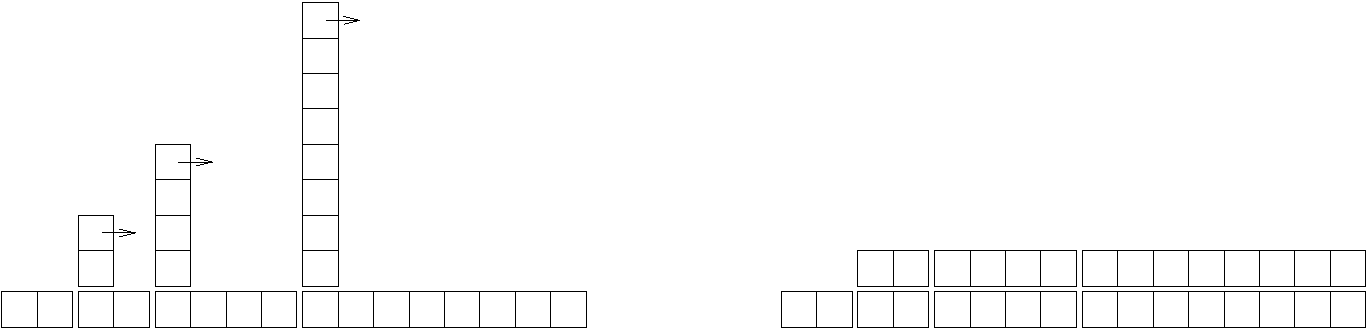
\includegraphics[width=5.5in]{figs/towers.pdf}}
\caption{雜湊表元素添加成本圖.\label{fig.hash}}
\end{figure}

再哈希所需要的額外消耗, 彷若一系列間距不斷增加, 同時高度不斷增長的高塔.
如果你推倒這些塔, 將調整空間大小的成本分攤到所有添加操作上, 
你可以從圖中明顯看到, $n$次添加操作的總成本為$2n-n$.

這個算法的一個重要特性是, 當我們調整雜湊表大小時, 其耗時呈幾何方式增長;
也就是說, 其大小乘以一個常數.
如果你增大其規模---每次增加固定數量---每次{\tt add}的平均耗時便是線性的.
\index{geometric resizing}

你可以從\url{http://thinkpython2.com/code/Map.py}下載我的雜湊表的實現代碼,
但請記住, 沒有必要用它; 如果你想使用映射, 用Python的字典即可.

\section{術語表}

\begin{description}

\item[算法分析(analysis of algorithms):] 一種基於算法運行時間和/或所需空間, 比較算法優劣的方法. 
\index{analysis of algorithms}

\item[機器模型(machine model):] 一種計算機的簡化表達方式, 用來描述算法.
\index{machine model}

\item[最糟糕情況(worst case):] 令給定算法運行最慢(或耗費空間最大)的輸入.
\index{worst case}

\item[主導項(leading term):] 多項式中, 具有最高次冪的項.
\index{leading term}

\item[交點(crossover point):] 兩種算法需要相同運行時間或空間的問題規模.
\index{crossover point}

\item[增長量級(order of growth):] 在算法分析中, 可以看作相同增長模式的函數集合.
比如, 所有耗時為線性變化的函數, 都屬於同樣的增長量級.
\index{order of growth}

\item[大O表示法(Big-Oh notation):] 用來表示增長量級的符號;
比如, $O(n)$表示耗時線性增長的函數集合. 
\index{Big-Oh notation}

\item[線性的(linear):] 一種運行時間和問題規模成比例變化的算法,
至少對大規模問題是如此.
\index{linear}

\item[二次方(quadratic):] 運行時間是$n^2$的算法, 其中$n$是問題規模的一個度量. 
\index{quadratic}

\item[檢索(search):] 定位集合(串列或字典)中的元素或確認其不存在的過程.
\index{search}

\item[雜湊表(hashtable):] 一種資料結構, 用來表示鍵-值對的集合, 同時
可以用常數時間進行檢索.
\index{hashtable}

\end{description}


\printindex

\clearemptydoublepage
%\blankpage
%\blankpage
%\blankpage

\end{document}
